\documentclass[a4paper]{article}
\usepackage{vntex}
%\usepackage[english,vietnam]{babel}
%\usepackage[utf8]{inputenc}
\usepackage{mathptmx}[ptm]
%\usepackage[utf8]{inputenc}
%\usepackage[francais]{babel}
\usepackage{a4wide,amssymb,epsfig,latexsym,array,hhline,fancyhdr}
\usepackage[normalem]{ulem}
%\usepackage{soul}
\usepackage{changepage}
\usepackage[makeroom]{cancel}
\usepackage{amsmath}
\usepackage{amsthm}
\usepackage{multicol,longtable,amscd}
\usepackage{diagbox}%Make diagonal lines in tables
\usepackage{booktabs}
\usepackage{alltt}
\usepackage[framemethod=tikz]{mdframed}% For highlighting paragraph backgrounds
\usepackage{caption,subcaption}
\renewcommand{\normalsize}{\fontsize{13}{15}\selectfont}

\setlength{\arrayrulewidth}{0.5mm}
\setlength{\tabcolsep}{5pt}
\renewcommand{\arraystretch}{1.5}
\usepackage{makecell}
\usepackage{float}
\usepackage{lastpage}
\usepackage[lined,boxed,commentsnumbered]{algorithm2e}
\usepackage{enumerate}
\usepackage{color}
\usepackage{graphicx}							% Standard graphics package
\usepackage{array}
\usepackage{tabularx, caption}
\usepackage{multirow}
\usepackage{multicol}
\usepackage{rotating}
\usepackage{graphics}
\usepackage{geometry}
\usepackage{setspace}
\usepackage{epsfig}
\usepackage{tikz}
\usepackage{setspace}
\usepackage{titlesec}
\usepackage{float}
\onehalfspacing


\usetikzlibrary{arrows,snakes,backgrounds,calc}
\usepackage[unicode]{hyperref}
\hypersetup{urlcolor=blue,linkcolor=black,citecolor=black,colorlinks=true} 
\usepackage{listings}


% Định dạng cho section
\titleformat{\section}[block]
{\normalfont\LARGE\bfseries}{Chương \thesection \newline }{1em}{}

% Thay đổi cách số thứ tự được hiển thị
% \renewcommand{\thesection}{\arabic{section}}


% Chỉnh kích thước của subsection
\titleformat{\subsection}
  {\normalfont\Large\bfseries}{\thesubsection}{1em}{}
  
\titleformat{\subsubsection}
  {\normalfont\large\bfseries}{\thesubsubsection}{1em}{}
\usepackage[normalem]{ulem}
\usepackage{parskip}
\setlength{\parindent}{28pt}
\newtheorem{theorem}{{\bf Định lý}}
\newtheorem{property}{{\bf Tính chất}}
\newtheorem{proposition}{{\bf Mệnh đề}}
\newtheorem{corollary}[proposition]{{\bf Hệ quả}}
\newtheorem{lemma}[proposition]{{\bf Bổ đề}}
\theoremstyle{definition}
\newtheorem{exer}{Bài toán}

\def\thesislayout{	% A4: 210 × 297
	\geometry{
		a4paper,
		total={160mm,240mm},  % fix over page
		left=30mm,
		top=0mm,
	}
}
\def\thesisheadlayout{	% A4: 210 × 297
	\geometry{
		a4paper,
		total={160mm,240mm},  % fix over page
		left=30mm,
		top=0mm,
	}
}

\lstset{
language=R,
basicstyle=\footnotesize\sffamily,
commentstyle=\ttfamily\color{black},
numbers=left,
numberstyle=\ttfamily\color{black}\footnotesize,
stepnumber=1,
numbersep=5pt,
backgroundcolor=\color{white},
showspaces=false,
showstringspaces=false,
showtabs=false,
frame=single,
tabsize=2,
captionpos=b,
breaklines=true,
breakatwhitespace=false,
title=\lstname,
escapeinside={},
keywordstyle={},
morekeywords={}
}
%\usepackage{fancyhdr}
\setlength{\headheight}{40pt}
\pagestyle{fancy}
\fancyhead{} % clear all header fields
\fancyhead[L]{
 \begin{tabular}{rl}
    \begin{picture}(25,15)(0,0)
    \put(0,-8){
\includegraphics[width=10mm, height=10mm]{Images/hcmut.png}}
    %\put(0,-8){\epsfig{width=10mm,figure=hcmut.eps}}
   \end{picture}&
	%\includegraphics[width=8mm, height=8mm]{hcmut.png} & %
	\begin{tabular}{l}
		\textbf{  Trường Đại Học Bách Khoa - Đại học Quốc gia TP.HCM }\\
		\textbf{  Khoa Khoa Học \& Kỹ Thuật Máy Tính}
	\end{tabular} 	
 \end{tabular}
}
\fancyhead[R]{
	\begin{tabular}{l}
		\tiny \bf \\
		\tiny \bf 
	\end{tabular}  }
\fancyfoot{} % clear all footer fields
\fancyfoot[L]{\scriptsize  Báo cáo Đồ án Tốt nghiệp (CO4337) - HK232}
\fancyfoot[R]{\scriptsize  Trang {\thepage}/\pageref{LastPage}}
\renewcommand{\headrulewidth}{0.3pt}
\renewcommand{\footrulewidth}{0.3pt}


%%%
\setcounter{secnumdepth}{4}
\setcounter{tocdepth}{3}
\makeatletter
\newcounter {subsubsubsection}[subsubsection]
\renewcommand\thesubsubsubsection{\thesubsubsection .\@alph\c@subsubsubsection}
\newcommand\subsubsubsection{\@startsection{subsubsubsection}{4}{\z@}%
                                     {-3.25ex\@plus -1ex \@minus -.2ex}%
                                     {1.5ex \@plus .2ex}%
                                     {\normalfont\normalsize\bfseries}}
\newcommand*\l@subsubsubsection{\@dottedtocline{3}{10.0em}{4.1em}}
\newcommand*{\subsubsubsectionmark}[1]{}
\makeatother

\everymath{\color{black}}%make in-line maths symbols blue to read/check easily

\sloppy
\captionsetup[figure]{labelfont={normalsize,bf},textfont={normalsize,it},belowskip=-1pt,aboveskip=-9pt}
%space remove between caption, figure, and text
\captionsetup[table]{labelfont={normalsize,bf},textfont={normalsize,it},belowskip=-1pt,aboveskip=7pt}
\setlength{\floatsep}{5pt plus 2pt minus 2pt}
\setlength{\textfloatsep}{5pt plus 2pt minus 2pt}
\setlength{\intextsep}{10pt plus 2pt minus 2pt}

\newcommand\tab[1][1cm]{\hspace*{#1}}

\begin{document}
\newgeometry{a4paper,
		total={160mm,260mm},  % fix over page
		left=30mm,
		top=10mm,
            ignorefoot
  }
\begin{titlepage}
% \begin{tikzpicture}[remember picture, overlay]
%   \draw[line width = 4pt] ($(current page.north west) + (2cm,-0.5in)$) rectangle ($(current page.south east) + (-0.4in,0.5in)$);
%   \draw[line width=1.5pt]
%     ($ (current page.north west) + (2.15cm,-0.55in) $)
%     rectangle
%     ($ (current page.south east) + (-0.45in,0.55in) $);
% \end{tikzpicture}

\begin{center}

\Large \textbf{ĐẠI HỌC QUỐC GIA TP.HCM} \\
\vspace{0.1cm}
\Large \textbf{TRƯỜNG ĐẠI HỌC BÁCH KHOA} \\
\vspace{0.1cm}
\Large \textbf{KHOA KHOA HỌC VÀ KĨ THUẬT MÁY TÍNH}
\end{center}

\vspace{0.3cm}

\begin{figure}[h!]
\begin{center}

\includegraphics[width=6cm]{Images/hcmut.png}
\end{center}
\end{figure}
\vspace{1cm}
\begin{center}
{{\Large \textbf{BÁO CÁO} }}\\
\vspace{0.1cm}
{\Large \textbf{ĐỒ ÁN TỐT NGHIỆP}}
\begin{tabular}{c}

\\{\textbf{{\LARGE PHÁT TRIỂN HỆ THỐNG }}}
\\{\textbf{{\LARGE QUẢN LÝ VÀ HỖ TRỢ BÁN THỜI TRANG }}}
\\{\Large NGÀNH: KHOA HỌC MÁY TÍNH}
\\
\\
\end{tabular}
\end{center}


\begin{table}[h]
\begin{tabular}{rll}
\hspace{5 cm} &  \textbf{\Large HỘI ĐỒNG:} {\Large Hội đồng 13 Khoa học Máy Tính}
\\
\hspace{3 cm} &   \textbf{\Large GVHD:} {\Large TS. Phan Trọng Nhân} 
\\
\hspace{3 cm}  &   \textbf{\Large GVPB:} {\Large TS. Nguyễn Thị Ái Thảo}
\\
% TKHĐ là THƯ KÝ HỘI ĐỒNG
\hspace{3 cm} &     \textbf{$\;$ $\;$$\;$$\;$$\;$$\;$$\;$$\;$$\;$$\;$$\;$$\;$$\;$$\;$$\;$$\;$$\;$$\;$$\;$$\;$$\;$$\;$$\;$$\;$$\;$$\;$$\;$$\;$$\;$$\;$$\;$$\;$$\;$$\;$ \Large ---o0o---} 
\\
\hspace{3 cm} &   \textbf{\Large SVTH1:} {\Large Nguyễn Tuấn Quyến - 2014311}
\\
\hspace{3 cm}&   \textbf{\Large SVTH2:}  {\Large Nguyễn Kim Tiến - 2014721}
\\
\hspace{3 cm} &   \textbf{\Large SVTH3:}  {\Large Lê Quốc Trạng - 2014812}
\\
\end{tabular}
\end{table}

\vspace{2cm}
\begin{center}
\Large \textbf{TP. HỒ CHÍ MINH, 6/2024}
\end{center}
\end{titlepage}




\newpage
\newgeometry{a4paper,
		total={160mm,240mm},  % fix over page
		left=30mm,
		top=30mm,
  }

\begin{center}
    \textbf{Lời cam đoan}
\end{center}

Chúng tôi xin cam đoan rằng hệ thống mà chúng tôi triển khai là độc lập và chỉ thuộc sở hữu của nhóm tôi, đồng thời được hướng dẫn bởi Tiến sĩ Phan Trọng Nhân. Các nội dung nghiên cứu và thiết kế đề tài này là trung thực, không sao chép hoặc sử dụng kết quả từ bất kỳ đề tài nào khác có tính tương tự.

Chúng tôi cam kết chịu trách nhiệm hoàn toàn về nội dung đồ án tốt nghiệp của mình và sẵn sàng chấp nhận mọi hình thức kỷ luật nếu phát hiện bất kỳ hành vi gian lận nào. Chúng tôi sẽ tuân thủ mọi quy tắc và quy định được đặt ra, và sẵn lòng chịu trách nhiệm trước Ban chủ nhiệm Khoa và Ban giám hiệu của nhà trường.

\newpage
\begin{center}
    \textbf{Lời cảm ơn}
\end{center}

Trong quá trình thực hiện đề tài đồ án tốt nghiệp, chúng tôi nhận được sự hỗ trợ đặc biệt từ nhiều nguồn. Đầu tiên và quan trọng nhất là giảng viên hướng dẫn trực tiếp của nhóm, Tiến sĩ Phan Trọng Nhân. Thầy đã tận tâm theo dõi, hướng dẫn và hỗ trợ chúng tôi không chỉ trong khía cạnh kiến thức chuyên môn mà còn chia sẻ những kinh nghiệm thực tế và lời khuyên hữu ích.

Chúng tôi xin chân thành cảm ơn sự hỗ trợ và sự giúp đỡ của TS. Phan Trọng Nhân cùng với tất cả các giảng viên, bạn bè và người thân đã đóng góp ý kiến, động viên và hỗ trợ chúng tôi trong quá trình thực hiện đề tài này. Đó là động lực lớn giúp chúng tôi vượt qua những thách thức và khó khăn.

% \newpage
% \begin{center}
%     \textbf{Tóm tắt}
% \end{center}

\newpage
\tableofcontents
\newpage
\listoffigures
\newpage
\listoftables
\newpage
\section{Tổng quan đề tài}
\subsection{Giới thiệu}
\indent \indent Trong thời đại số hóa ngày càng phát triển, việc mua sắm trực tuyến đã trở thành một phần quan trọng của cuộc sống hàng ngày của chúng ta. Với sự tiến bộ của công nghệ và sự phát triển của internet, các hệ thống mua hàng hiện nay đã thay đổi cách chúng ta mua sắm và tiêu dùng.

Ngành bán lẻ hiện nay đã chứng kiến một cuộc biến đổi đáng kể trong cách tiếp cận bán hàng và quảng cáo. Trước đây, mô hình bán lẻ truyền thống thường giới hạn việc phân phối sản phẩm thông qua một số cửa hàng và trung tâm thương mại, tạo ra rào cản lớn đối với các doanh nghiệp mới muốn đưa sản phẩm của họ đến tay người tiêu dùng. Tuy nhiên hiện nay, việc mua sắm trực tuyến đã trở nên phổ biến và phát triển mạnh mẽ, không còn xa lạ đối với chúng ta, đặc biệt là với giới trẻ.

Mua sắm trực tuyến đã đem lại một loạt lợi ích cho cả người tiêu dùng và doanh nghiệp. Điều này bao gồm sự thuận tiện, đa dạng sản phẩm, khả năng tiếp cận thị trường toàn cầu, và cơ hội tạo ra trải nghiệm mua sắm cá nhân hóa dựa trên dữ liệu. Điều này đã thúc đẩy nhiều doanh nghiệp mở rộng hoạt động kinh doanh của họ trực tuyến và tận dụng các kênh trực tuyến để tương tác và làm ấn tượng với khách hàng.

Tuy nhiên, với sự gia tăng của mô hình kinh doanh trực tuyến, cạnh tranh cũng trở nên khốc liệt hơn. Điều này đặt ra áp lực lớn đối với doanh nghiệp phải không ngừng cải thiện sản phẩm, dịch vụ, và chiến lược tiếp thị để duy trì và tăng cường sự hấp dẫn đối với khách hàng. Đồng thời, quản lý dữ liệu và bảo mật thông tin cá nhân của khách hàng cũng trở thành một phần quan trọng trong hoạt động kinh doanh trực tuyến.

Hệ thống bán hàng và quản lý cửa hàng thời trang mà chúng tôi phát triển sẽ giúp cho doanh nghiệp có thể quản lý được các mặt hàng thời trang, tích hợp cổng thanh toán, theo dõi được các đơn hàng, doanh thu và các chi phí khác. Ngoài ra còn phát triển thêm một ứng dụng di động để người dùng có thể mua hàng trực tuyến.
\subsection{Mục tiêu}
\indent \indent Mục tiêu của chúng tôi trong việc phát triển hệ thống quản lý và hỗ trợ bán hàng thời trang là tạo ra một ứng dụng trên nền tảng di động, mang lại trải nghiệm mua sắm thân thiện, thú vị và hiệu quả cho người dùng. Chúng tôi kỳ vọng rằng thông qua việc xây dựng ứng dụng di động này, chúng tôi sẽ giúp người dùng dễ dàng tìm kiếm và thực hiện mua sắm thời trang một cách thuận tiện, đồng thời cung cấp cho họ các công cụ và tính năng để cải thiện phong cách thời trang cá nhân và tăng cường trải nghiệm mua sắm.

Cụ thể, đồ án tốt nghiệp nhắm đến các mục tiêu:
\begin{itemize}
\item{Xây dựng một hệ thống gợi ý thông minh dựa trên dữ liệu mua sắm và sở thích của khách hàng, có khả năng dự đoán và đề xuất các sản phẩm thời trang phù hợp với từng cá nhân, tạo điều kiện thuận lợi cho khách hàng mua sắm và tăng cường trải nghiệm mua sắm.}
\item{Cho phép khách hàng thanh toán bằng các phương thức tiền điện tử phổ biến như ví điện tử, và ngân hàng giúp thuận tiện cho khách hàng và phù hợp với xu hướng thanh toán ngày càng phổ biến.}
\item{Phân tích dữ liệu để thu thập, xử lý và phân tích thông tin về doanh số bán hàng, sự phổ biến của sản phẩm và hành vi mua sắm của khách hàng, giúp cửa hàng đưa ra các quyết định kinh doanh hiệu quả.}

\item{Xây dựng giao diện đa ngôn ngữ để cung cấp trải nghiệm mua sắm thuận tiện cho khách hàng quốc tế. Bằng cách hỗ trợ nhiều ngôn ngữ, cửa hàng có thể thu hút và giữ chân nhiều khách hàng từ các quốc gia khác nhau.}

\item{Xây dựng tính năng cho phép khách hàng đánh giá và viết nhận xét về sản phẩm đã mua. Điều này giúp cung cấp thông tin đáng tin cậy cho những khách hàng khác và tăng tính minh bạch của cửa hàng.}

\item{Xây dựng tính năng kiểm duyệt nội dung đánh giá sản phẩm. Điều này giúp bảo vệ không gian đánh giá sản phẩm khỏi các nội dung tiêu cực và giữ cho trải nghiệm của người dùng được an toàn và tích cực}

\end{itemize}

Ngoài ra, mục tiêu của đề tài cũng là tìm hiểu và áp dụng các công nghệ mới nhất trong lĩnh vực phát triển web/app, bao gồm cả ReactJS, Postgresql, AWS, React Native và các công nghệ khác để tạo ra một nền tảng mạnh mẽ, hiệu quả và bảo mật.

Bằng cách tạo ra ứng dụng di động này, chúng tôi hy vọng rằng người dùng sẽ có cơ hội trải nghiệm không chỉ sự thuận tiện trong việc mua sắm thời trang mà còn khám phá và thử nghiệm các xu hướng thời trang mới. Đồng thời, chúng tôi cũng hướng đến việc cung cấp thông tin chi tiết và đánh giá sản phẩm để giúp người dùng có lựa chọn thông minh và hài lòng. Mục tiêu của chúng tôi không chỉ dừng lại ở việc tạo ra một ứng dụng di động hoàn hảo cho mua sắm thời trang, mà còn là việc đóng góp vào sự phát triển của ngành công nghiệp thời trang và cộng đồng mua sắm. Chúng tôi tin rằng việc phát triển ứng dụng này sẽ mang lại lợi ích lớn cho xã hội và đất nước, đồng thời giúp thúc đẩy sự phát triển và nâng cao uy tín của ngành thời trang.
\subsection{Phạm vi đề tài}
Phạm vi của đề tài "PHÁT TRIỂN HỆ THỐNG QUẢN LÝ VÀ HỖ TRỢ BÁN THỜI TRANG" sẽ bao gồm các khía cạnh công nghệ liên quan đến phát triển ứng dụng di động, gồm thiết kế giao diện người dùng, phát triển ứng dụng di động, quản lý cơ sở dữ liệu, tích hợp thanh toán trực tuyến, và phân tích dữ liệu.

Về phạm vi đối tượng người dùng, ứng dụng di động này sẽ được thiết kế để phục vụ khách hàng trong lĩnh vực thời trang. Đối tượng người dùng mà chúng tôi nhắm tới bao gồm những người yêu thời trang và có nhu cầu mua sắm sản phẩm thời trang. Ứng dụng sẽ giúp họ tìm kiếm, chọn lựa, và mua sắm các sản phẩm thời trang một cách thuận tiện và hiệu quả. Đồng thời, ứng dụng sẽ hỗ trợ các nhân viên cửa hàng trong việc quản lý hàng tồn kho và tương tác với khách hàng.

Ứng dụng này không dành cho người dùng không có kiến thức về thời trang hoặc tin học. Chúng tôi mục tiêu phục vụ những người có sự quan tâm đến thời trang và có kiến thức cơ bản về mua sắm trực tuyến và ứng dụng di động.
\subsection{Kế hoạch}
Đề tài chúng tôi bao gồm các bước chính như sau:

\textbf{Bước 1. Nghiên cứu và đánh giá hệ thống hiện có:}

Trong giai đoạn này, chúng tôi đã dành thời gian để tìm hiểu và đánh giá các hệ thống tương tự đã tồn tại trên thị trường. Chúng tôi xem xét những ưu điểm và nhược điểm của mỗi hệ thống này để có cơ sở đề xuất những cải tiến và giải pháp tốt hơn cho hệ thống quản lý và hỗ trợ bán hàng thời trang của chúng tôi.

\textbf{Bước 2. Xây dựng kiến trúc và thiết kế giao diện:}

Sau khi hoàn thành giai đoạn nghiên cứu và đánh giá, chúng tôi tiến hành xây dựng kiến trúc tổng thể của hệ thống, bao gồm việc thiết kế cơ sở dữ liệu, giao diện người dùng, và xây dựng các giao diện lập trình ứng dụng (API).

\textbf{Bước 3. Phát triển các tính năng và chức năng cơ bản:}

Trong giai đoạn này, chúng tôi bắt đầu phát triển các tính năng và chức năng cơ bản cho hệ thống quản lý và hỗ trợ bán hàng thời trang. Điều này bao gồm việc tạo ra các tính năng như đăng ký tài khoản, tạo hồ sơ cá nhân và nhiều chức năng quan trọng khác.

\textbf{Bước 4. Tối ưu hóa và kiểm tra}

Sau khi hoàn thành phần phát triển cơ bản, chúng tôi tiến hành tối ưu hóa và kiểm tra hệ thống. Điều này bao gồm việc kiểm tra và khắc phục lỗi, cải thiện hiệu suất của hệ thống và tăng cường tính bảo mật để đảm bảo tính ổn định và an toàn.

\textbf{Bước 5. Phát triển các tính năng và chức năng mở rộng:}

Sau khi hoàn thành các tính năng và chức năng cơ bản, chúng tôi tiếp tục phát triển và mở rộng hệ thống. Điều này bao gồm việc thêm các tính năng mới, cải thiện trải nghiệm người dùng và đáp ứng các yêu cầu mở rộng của khách hàng và thị trường.

Đối với phía ứng ụng di động, chúng tôi sẽ tiến hành gỡ lỗi và tối ưu hoá ứng dụng trên cả 2 nền tảng Android và IOS, sau đó sẽ phát triển thêm một số chức năng cần thiết khác như thông báo ứng dụng.

Đối với phía hệ thống, chúng tôi sẽ tối ưu hoá các truy vấn và cơ sở dữ liệu, sẽ xây dựng thêm một số chức năng khác như liên kết thẻ thanh toán, chat box hỗ trợ khách hàng...



\newpage
\section{Kiến thức nền tảng}
\subsection{Khảo sát thực tế}
\subsubsection{H\&M}

\indent \indent H\&M (Hennes \& Mauritz AB) là một tập đoàn thời trang quốc tế có trụ sở tại Thụy Điển. H\&M có mặt trên toàn thế giới và chuyên cung cấp các sản phẩm thời trang cho nam, nữ và trẻ em.

H\&M đã phát triển ứng dụng di động dành cho khách hàng có tên là "H\&M". Ứng dụng này cung cấp trải nghiệm mua sắm thuận tiện, cho phép người dùng duyệt qua các sản phẩm, thực hiện đặt hàng và nhận thông tin về khuyến mãi và xu hướng thời trang.
\subsubsection{Zalora}
\indent \indent Zalora là một công ty thương mại điện tử chuyên về thời trang có hoạt động rộng khắp khu vực Đông Nam Á.

Zalora cung cấp một ứng dụng di động cho phép khách hàng duyệt qua và mua sắm các sản phẩm thời trang từ các thương hiệu nổi tiếng.

Ứng dụng Zalora cung cấp các tính năng như tìm kiếm sản phẩm, xem chi tiết sản phẩm, đặt hàng và thanh toán trực tuyến.
\subsubsection{Cider}
\indent \indent Cider là một ứng dụng di động bán hàng thời trang phổ biến. Ứng dụng này cung cấp một nền tảng tương tác giữa người bán và người mua, cho phép người dùng tạo và quản lý cửa hàng trực tuyến của riêng mình.

Cider hỗ trợ việc tạo và quản lý danh mục sản phẩm, xử lý thanh toán, và tương tác với khách hàng thông qua hệ thống chat tích hợp.

\subsubsection{So sánh giữa các ứng dụng}
\begin{center}
\begin{longtable}{ |p{3cm}|p{3cm}|p{3cm}|p{3cm}| }
\hline
\textbf{Các tiêu chí}  & \textbf{H\&M \cite{HM}} & \textbf{ZALORA \cite{zalora}} & 
\textbf{CIDER \cite{cider}} \\
\hline
\endfirsthead

\hline
\textbf{Các tiêu chí}  & \textbf{H\&M \cite{HM}} & \textbf{ZALORA \cite{zalora}} & 
\textbf{CIDER \cite{cider}} \\
\hline
\endhead

\raggedright Giao diện người dùng (UI) và trải nghiệm người dùng (UX) &  Hiện đại và thân thiện với người dùng & Đẹp, dễ sử dụng, tốc độ phản hồi nhanh & Thiết kế đẹp, dễ sử dụng\\
\hline
\raggedright Tính năng sản phẩm & Đa dạng, xu hướng thời trang nhanh & Nhiều thương hiệu quốc tế và địa phương &Đa dạng, thời trang nhanh dành cho phụ nữ\\
\hline
\raggedright Tích hợp thanh toán và giao hàng & Thuận tiện & Có đầy đủ các tích hợp thanh toán & Có tích hợp thanh toán và giao hàng\\
\hline
\raggedright Tương tác xã hội và đánh giá & Không tích hợp xem đánh giá sản phẩm & Tích hợp đánh giá và phản hồi khách hàng & Tích hợp xem đánh giá sản phẩm, chia sẻ mạnh mẽ trên mạng xã hội\\
\hline
\raggedright Hiệu suất và tốc độ & Ứng dụng hoạt động mượt mà & Ứng dụng hoạt động mượt mà & Ứng dụng hoạt động mượt mà \\
\hline
\raggedright Tính năng tương tác & Danh sách mong muốn, lịch sử mua sắm, thông báo & Danh sách mong muốn, lịch sử mua sắm, thông báo & Có danh sách ưa thích. Không có thử đồ trực tuyến, tư vấn khác thời trang \\
\hline
\raggedright Hỗ trợ khách hàng & Trung tâm trợ giúp, chat trực tiếp, email & Có hỗ trợ khách hàng trực tuyến & Không có hỗ trợ khách hàng\\
\hline
\raggedright Tìm kiếm thông minh & Theo tên, danh mục, bộ sưu tập & Dựa theo từ khóa tìm kiếm nhiều nhất & Dựa theo từ khóa\\
\hline
\raggedright Hệ thống gợi ý mua hàng & Dựa trên lịch sử mua sắm & Dựa trên lịch sử mua sắm & Dựa trên lịch sử mua sắm \\
\hline
\caption{Bảng so sánh các tiêu chí}
\end{longtable}
\end{center}
Mô tả các tiêu chí:
\begin{itemize}
    \item Giao diện người dùng (UI) và trải nghiệm người dùng (UX): Đánh giá cách ứng dụng được thiết kế và cách người dùng tương tác với nó. Giao diện nên dễ sử dụng, hấp dẫn và phản ánh thương hiệu.

 \item Tính năng sản phẩm: Đảm bảo rằng ứng dụng cung cấp đầy đủ thông tin về sản phẩm, bao gồm hình ảnh, mô tả chi tiết và giá cả. Các tính năng như tìm kiếm, lọc sản phẩm và đánh giá sản phẩm cũng nên được cung cấp.

\item Tích hợp thanh toán và giao hàng: Kiểm tra tính năng thanh toán an toàn và đa dạng cùng với tùy chọn giao hàng linh hoạt. Bảo đảm rằng thông tin thanh toán của khách hàng được bảo vệ.

\item Tương tác xã hội và đánh giá: Ứng dụng nên cho phép khách hàng đăng nhận xét và đánh giá sản phẩm. Cung cấp tích hợp xã hội để chia sẻ sản phẩm và khuyến mãi.

\item Tính năng tương tác: Cân nhắc tích hợp tính năng thử đồ trực tuyến, hoặc tạo các chức năng tương tác khác như tư vấn thời trang hoặc danh sách ưa thích.

\item Tính năng phân tích và theo dõi: Đánh giá khả năng theo dõi hoạt động của người dùng, thống kê doanh số bán hàng, và sử dụng các công cụ phân tích để cải thiện chiến lược kinh doanh.

\item Bảo mật và quyền riêng tư: Đảm bảo rằng thông tin cá nhân của khách hàng được bảo vệ một cách an toàn và tuân thủ các quy định về quyền riêng tư.

\item Hiệu suất và tốc độ: Ứng dụng nên hoạt động một cách nhanh chóng và mượt mà trên các thiết bị khác nhau.

\item Hỗ trợ khách hàng: Cung cấp các kênh hỗ trợ khách hàng như chat trực tuyến, email hoặc số điện thoại để giải quyết thắc mắc và vấn đề của khách hàng.

\item Tích hợp mạng xã hội và tiếp thị: Đánh giá khả năng chia sẻ trên mạng xã hội và các chiến dịch tiếp thị trên ứng dụng.

\item Tuân thủ quy định: Đảm bảo rằng ứng dụng tuân thủ tất cả các quy định và luật pháp liên quan đến kinh doanh trực tuyến và bán hàng.
\end{itemize}

% \subsection{Các khái niệm trong hệ thống}

\subsection{Cơ sở lý thuyết}
\subsubsection{Kiến trúc phân lớp (Layered Architecture)}
\indent \indent Kiến trúc phân lớp là một phương pháp tổ chức và xây dựng hệ thống phần mềm, trong đó các thành phần được chia thành các lớp riêng biệt với vai trò và trách nhiệm cụ thể. Mỗi lớp đảm nhận một phần công việc cụ thể và tương tác với các lớp khác thông qua giao diện định nghĩa rõ ràng.

\begin{figure}[H]
    \centering
    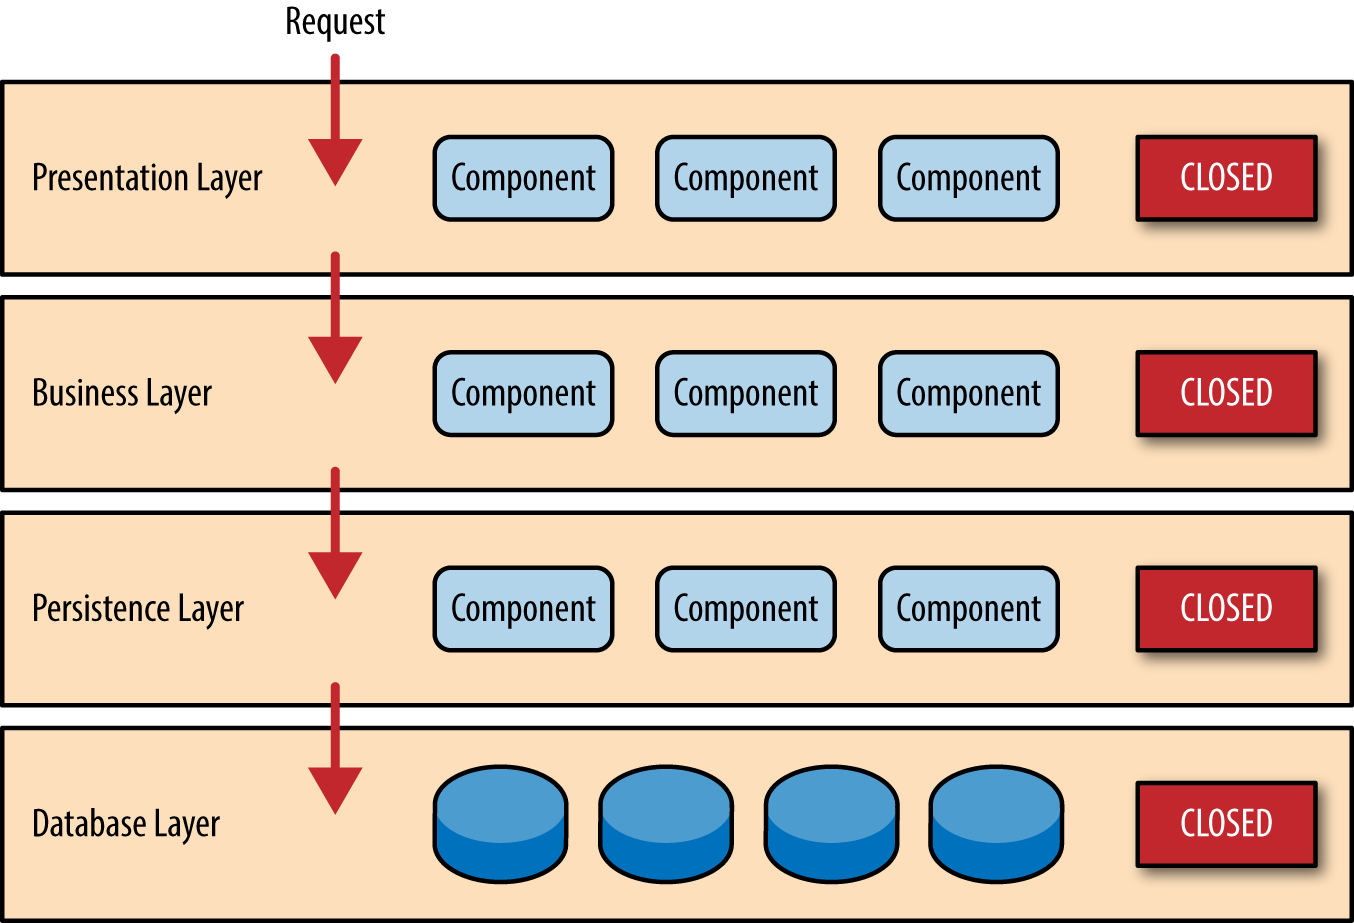
\includegraphics[width=15cm]{Images/Technology/layer_ar.png}
    \vspace{1cm}
    \caption{Four Layered Architecture \cite{layerd}}
\end{figure}

\noindent Trong kiến trúc phân lớp, hệ thống được chia thành ba lớp chính:
\begin{itemize}
    \item \textbf{Presentation layer} (lớp giao diện): Đây là lớp mà người dùng tương tác trực tiếp. Nó xử lý việc hiển thị dữ liệu và tương tác với người dùng thông qua giao diện người dùng.
    \item \textbf{Business layer} (lớp logic): Lớp này chứa các quy tắc nghiệp vụ và xử lý logic của hệ thống. Nó đảm bảo tính logic và tính toàn vẹn của dữ liệu.
    \item \textbf{Data layer} (lớp dữ liệu): Lớp này quản lý truy cập và tương tác với cơ sở dữ liệu. Nó cung cấp các phương thức để lấy và lưu trữ dữ liệu.
\end{itemize}
Trong dự án này chúng tôi sẽ dùng thêm một lớp là 
\textbf{Persistence Layer}, thường là một phần của Business Layer. Nó cung cấp các dịch vụ để tương tác với cơ sở dữ liệu, bao gồm các hoạt động như truy vấn, cập nhật, xóa và tạo mới dữ liệu. Qua tầng này, các thành phần trong Business Layer có thể giao tiếp với cơ sở dữ liệu một cách đơn giản và trừu tượng hóa. Với việc gọi Persistence Layer, chúng ta có thể truy xuất và sửa đổi dữ liệu trong cơ sở dữ liệu một cách dễ dàng và linh hoạt. Chúng tôi có sử dụng các công nghệ như ORM (Object-Relational Mapping) và OGM (Object-Graph Mapping) để tạo ra các đối tượng và ánh xạ chúng thành dữ liệu trong cơ sở dữ liệu. Điều này giúp tách biệt logic kinh doanh và tương tác với cơ sở dữ liệu, tạo ra một kiến trúc dễ bảo trì và mở rộng.
Các lớp trong kiến trúc phân lớp được tổ chức theo cách mà mỗi lớp chỉ phụ thuộc vào lớp ngay dưới nó, và không phụ thuộc vào lớp ngay trên nó. Điều này giúp tách biệt các công việc và trách nhiệm của từng lớp và dễ dàng thay đổi và bảo trì hệ thống.

Kiến trúc phân lớp giúp tăng tính linh hoạt, tái sử dụng và bảo trì của hệ thống phần mềm. Nó cũng giúp tách biệt các quy tắc nghiệp vụ và giao diện người dùng, làm cho hệ thống dễ dàng mở rộng và thay đổi theo yêu cầu của người dùng.
\subsubsection{RESTful API}
RESTful API (Representational State Transfer - Application Programming Interface) là một kiến trúc thiết kế API dựa trên các nguyên tắc của REST, giúp tạo ra các dịch vụ web mạnh mẽ, linh hoạt và dễ hiểu. RESTful API thường được sử dụng để tương tác với cơ sở dữ liệu và tạo ra các ứng dụng web hoặc di động.\\
Đặc Điểm và Tính Năng Chính của RESTful API:
\begin{itemize}
\item HTTP Methods: RESTful API sử dụng các phương thức HTTP như GET, POST, PUT, PATCH, và DELETE để thực hiện các thao tác trên tài nguyên. Mỗi phương thức có ý nghĩa và mục đích riêng.
\item Stateless Communication: Giao tiếp trong RESTful API là stateless, điều này có nghĩa là mỗi yêu cầu từ client đều chứa đủ thông tin cần thiết để server hiểu và xử lý mà không cần dựa vào bất kỳ trạng thái nào từ trước đó.
\item Resource-Based: Mọi thứ trong RESTful API được xem như một tài nguyên và được định danh bằng các URI (Uniform Resource Identifier). Điều này giúp dễ dàng quản lý và tìm kiếm các tài nguyên.
\item Representation: Dữ liệu của tài nguyên được truyền tải giữa client và server dưới dạng các biểu diễn (representation) như JSON hoặc XML. Điều này giúp tương thích và linh hoạt.
\item HATEOAS (Hypermedia As The Engine Of Application State): RESTful API có thể cung cấp các liên kết hypermedia trong các phản hồi, giúp client hiểu được các hành động mà nó có thể thực hiện tiếp theo.
\item Versioning: RESTful API thường hỗ trợ việc quản lý phiên bản để đảm bảo tính tương thích giữa các phiên bản khác nhau của API.
\item Authentication và Authorization: RESTful API hỗ trợ các phương thức xác thực và phân quyền để đảm bảo an toàn và bảo mật thông tin.
\item Caching: RESTful API có thể sử dụng các cơ chế caching để tối ưu hóa hiệu suất, giảm tải cho server, và giảm thời gian đáp ứng\\
RESTful API đã trở thành một tiêu chuẩn phổ biến trong việc xây dựng các dịch vụ web và ứng dụng di động, đặc biệt là khi cần sự tương thích và khả năng mở rộng.
\end{itemize}
\subsubsection{Json Web Token}
\begin{figure}[h]
    \centering
    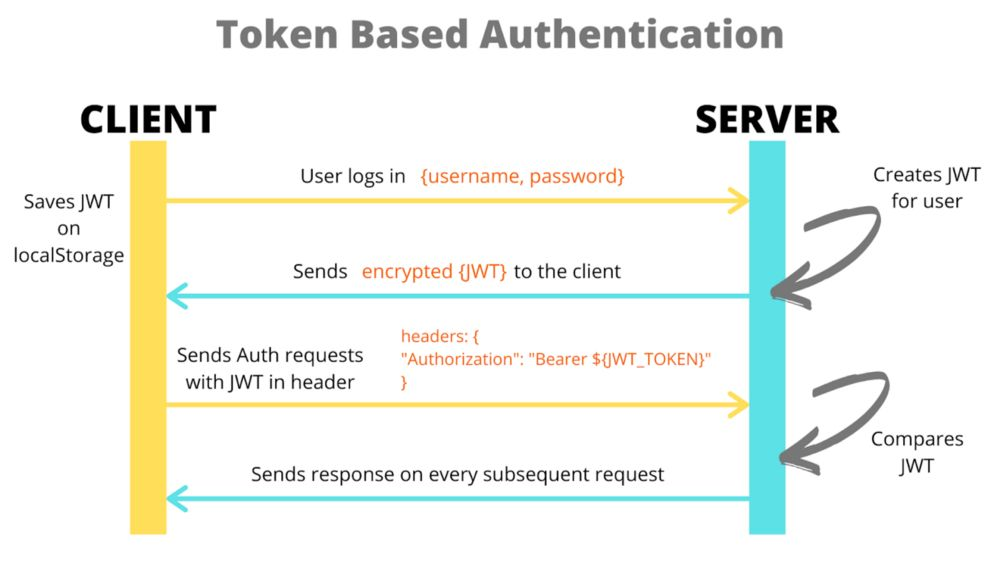
\includegraphics[width=10cm]{Images/Technology/jwt.png}
    \vspace{10pt}
    \caption{Json Web Token \cite{jsonwebtoken}}
\end{figure}

JSON Web Token (JWT) là một tiêu chuẩn mở định nghĩa một cách ngắn gọn và khép kín
để truyền dẫn thông tin giữa hai bên client và server được định dạng bằng JSON.\\
Chuỗi JWT gồm 3 thành phần là header, payload, signature và được ngăn cách nhau bằng
dấu chấm ("."). Do đó, một chuỗi JWT có dạng như sau:
\begin{center}
    \textbf{header.payload.signature}
\end{center}
\begin{itemize}
    \item \textbf{Header}: Phần header thường chứa hai phần là kiểu dữ liệu (giá trị thường là JWT) và thuật toán sử dụng để mã hóa chuỗi như HMAC SHA256 hoặc RSA.
    \item \textbf{Payload}:Phần payload chứa thông tin muốn đặt trong chuỗi như tên đăng nhập (username), id của người dùng (user id), tên người dùng,...
    \item \textbf{Signature}: Phần signature sẽ được tạo ra bằng cách mã hóa phần header và payload kèm theo một chuỗi được gọi là secret (khóa bí mật). Thuật toán để mã hóa được mô tả ở phần header.
    
\end{itemize}
\subsubsection{Graph}
\
\indentĐồ thị là một tập các đối tượng gọi là đỉnh nối với nhau bởi các cạnh. Thông thường, đồ thị được vẽ dưới dạng một tập các điểm (đỉnh, nút) nối với nhau bởi các đoạn thẳng (cạnh). Graph Database mô tả và lưu trữ dữ liệu dưới dạng đồ thị, một cách trực quan và dễ dàng truy vấn. Hiểu 1 cách đơn giản, graph database là database sử dụng cấu trúc graph để lưu trữ dữ liệu, nó khác so với cơ sỡ dữ liệu quan hệ lưu data dưới dạng bảng, hay NoSQL lưu data dưới dạng document key value.
\begin{figure}[h]
    \centering
    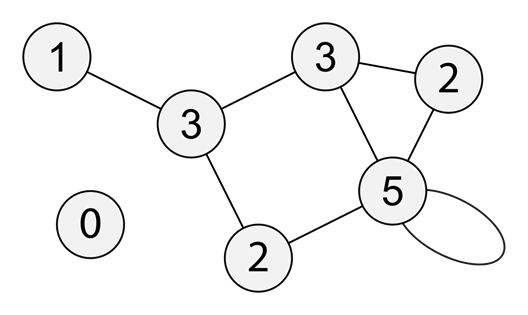
\includegraphics[width=7cm]{Images//Technology/graph.png}
    \vspace{10pt}
    \caption{Graph \cite{graph}}
    \label{fig:enter-label}
\end{figure}
\\
\noindent\textbf{Lợi ích của Graph}\\
\indent Bối cảnh hiện đại đặt ra rất nhiều bài toán cần phải giải quyết như: phát hiện gian lận tài chính, gợi ý bạn bè trên các nền tảng mạng xã hội, gợi ý một item cho người dùng dựa trên lịch sử hoạt động của người đó...\\
\indent Với những kiểu bài toán như vậy thì cách lưu trữ dữ liệu của Relational Database hoặc NoSQL Database đều không thích hợp khi mà chúng chỉ chuẩn hóa dữ liệu để lưu vào các bảng hay các document và làm giảm đi tính kết nối. Việc lưu trữ như vậy không thể tận dụng được hết sức mạnh của các mối liên kết có thể mang lại. Đặc biệt, việc truy vấn giữa các bảng rất phức tạp và mất nhiều thời gian.\\
Một minh chứng cho sự hữu ích của Graph Database đó chính là việc gợi ý kết bạn trên nền tảng mạng xã hội Facebook. Ví dụ, khi A là bạn của B và B là bạn của C, với công nghệ graph, Facebook sẽ biết được liệu có nên gợi ý kết bạn cho A và C hay không.\\
\noindent \textbf{Một số bài toán áp dụng Graph Database}
\begin{itemize}
    \item Xây dựng một hệ thống gợi ý mua hàng thông qua các mối quan hệ giữa người dùng A và B khi có điểm tương đồng trong việc mua sản phẩm.
    \item Phát hiện mối liên hệ giữa những người dùng có quen biết nhau, có tương tác giống nhau trên mạng xã hội.
    \item Phát hiện các hành vi vi phạm tài chính, ví dụ như hành vi rửa tiền khi chuyển khoản qua nhiều tài khoản, nhiều ngân hàng khác nhau.
    \item Gợi ý kết bạn dựa trên mối quan hệ bạn bè hiện có của tài khoản mạng xã hội
    \item Tối ưu đường bay của máy bay thương mại, tối ưu đường vận tải của các xe chở hàng

\end{itemize}
\subsection{Công nghệ}
\subsubsection{Công nghệ Frontend}
\begin{enumerate}[a. ]
\item \textbf{Typescript}\\
\begin{figure}[H]
    \centering
     
\includegraphics[scale=0.15]{Images/Technology/ts1.png}
     \caption{TypeScript \cite{typescript}}
\end{figure}
TypeScript là một ngôn ngữ lập trình mã nguồn mở được phát triển bởi Microsoft, và nó có thể được coi là một "mở rộng" của JavaScript. TypeScript được tạo ra để giúp việc phát triển ứng dụng JavaScript lớn và phức tạp trở nên dễ dàng hơn bằng cách thêm vào nó các khái niệm về kiểu dữ liệu tĩnh và các tính năng lập trình hướng đối tượng. \\
Đặc điểm và tính năng chính của TypeScript:
\begin{itemize}
\item Kiểu dữ liệu tĩnh: TypeScript giúp xác định rõ kiểu dữ liệu của biến, tham số hàm và giá trị trả về của hàm. Điều này giúp phát hiện lỗi kiểu tại thời điểm biên dịch thay vì tại thời điểm chạy, giúp tăng tính ổn định và tin cậy của ứng dụng.
\item Lập trình hướng đối tượng: TypeScript hỗ trợ các khái niệm lập trình hướng đối tượng như lớp, đối tượng, kế thừa, và các tính năng khác. Điều này giúp tạo ra mã nguồn dễ hiểu, tái sử dụng và bảo trì.
\item Tích hợp với JavaScript: TypeScript là siêu tập của JavaScript, nghĩa là mọi mã JavaScript hợp lệ đều là mã TypeScript. Điều này cho phép dự án chuyển từ JavaScript sang TypeScript một cách dễ dàng và mục tiêu đặt ra là giữ nguyên tương thích ngược.
\item Compiler: TypeScript có một trình biên dịch riêng biệt, giúp kiểm tra và chuyển đổi mã nguồn TypeScript thành mã nguồn JavaScript. Quá trình biên dịch này giúp kiểm soát lỗi và tối ưu hóa mã nguồn.
\end{itemize}

\item \textbf{ReactJs}\\
\begin{figure}[H]
    \centering
     
\includegraphics[scale=0.15]{Images/Technology/react.png}
     \vspace{10pt}
     \caption{React \cite{reactjs}}
\end{figure}
React JS là một thư viện JavaScript phổ biến do Facebook phát triển, dùng để xây dựng giao diện người dùng (UI).\\
Tính năng chính của React JS:
\begin{itemize}
\item Component-Based: React cho phép tạo các đơn vị UI tái sử dụng gọi là "Components," mỗi cái có logic và cấu trúc riêng, có thể tái sử dụng ở nhiều nơi khác nhau trong ứng dụng.
\item Hiệu suất: Sử dụng Virtual DOM để cập nhật và đồng bộ hóa trạng thái DOM hiệu quả, giúp cập nhật UI nhanh chóng và mượt mà.
\item JSX: React sử dụng cú pháp mở rộng của JavaScript, JSX, cho phép tích hợp logic và render markup trong cùng một component.
\item Kết hợp dễ dàng: React hoạt động tốt với các thư viện và framework khác, có thể sử dụng làm view layer trong các ứng dụng MVC.
\end{itemize}
\item \textbf{React Native}
\begin{figure}[H]
    \centering
     
\includegraphics[scale=0.3]{Images/Technology/reactNative.png}
     \vspace{10pt}
     \caption{React Native \cite{reactnative}}
     \label{fig:enter-label}
\end{figure}
React Native là một framework mã nguồn mở được phát triển bởi Facebook. Framework này giúp phát triển app mobile trên cả 2 hệ sinh thái iOS và Android một cách dễ dàng. Chính vì thế lập trình React Native sẽ giúp tiết kiệm được phần lớn thời gian và công sức khi thiết kế và xây dựng nên một ứng dụng đa nền tảng.\\\\
\textbf{Những ưu điểm của React Native}
\begin{itemize}
\item  Thời gian học React Native ngắn: 
React Native cung cấp giải pháp lập trình đa nền tảng. Thay vì tìm hiểu 2 hệ sinh thái các biệt của iOS và Android, chỉ tốn thời gian học React Native có thể phát triển tốt cho cả iOS và Android.
\item Có thể lập trình trên đa dạng hệ điều hành:
React Native là bước chuyển mình lớn của mobile app. Việc lập trình trên đa dạng hệ điều hành mang đến sự tiện ích cho cộng đồng dev trên toàn cầu.
\item Cộng đồng React Native lớn:
React Native được rất nhiều ông lớn trong ngành công nghệ đang sử dụng. Điều này giúp cho cộng đồng người học React Native phát triển mạnh mẽ.
\item Hot Reloading:
Với mỗi lập trình viên, thời gian Reload app sau mỗi chỉnh sửa nhỏ luôn là vấn đề khó chịu và tốn nhiều thời gian. Trong nhiều project với lượng source code lớn thì thời gian build, đóng gói và cài đặt lại luôn gây mệt mỏi đối với dev. Đặc biệt là trong giai đoạn dự án gấp rút.
\item Tăng trải nghiệm của người dùng:
Giao diện đơn giản, đa dạng ứng dụng, hoàn hảo trong thiết kế app… React Native tạo nên nhiều ứng dụng hữu ích cho người dùng. Hàng nghìn ứng dụng đang dùng React Native chính là minh chứng cho sự linh hoạt của ứng dụng từ React Native.
\end{itemize}
% \item \textbf{Flutter}
% \begin{figure}[H]
% \centering
%  
\includegraphics[scale=0.35]{Images/Technology/flutter.png}
% \end{figure}
% Flutter là một framework phát triển ứng dụng di động mã nguồn mở được phát triển bởi Google. Được giới thiệu vào năm 2017, Flutter nhanh chóng trở thành một lựa chọn phổ biến cho việc xây dựng ứng dụng di động đa nền tảng, với khả năng chia sẻ mã nguồn giữa các nền tảng khác nhau.\\
% Flutter sử dụng ngôn ngữ lập trình Dart và nổi bật với mô hình lập trình gọi là "reactive programming," trong đó giao diện người dùng được xây dựng dựa trên trạng thái và sự kiện. Framework này cung cấp một tập hợp đầy đủ các widget để xây dựng giao diện người dùng, giúp ứng dụng có giao diện thân thiện và đẹp mắt.\\
% Flutter cho phép phát triển ứng dụng không chỉ cho nền tảng di động (iOS và Android) mà còn cho web và desktop. Điều này mang lại sự linh hoạt và tiện ích trong việc đáp ứng nhu cầu ngày càng đa dạng của người phát triển.\\
% Đặc Điểm và Tính Năng Chính của Flutter:
% \begin{itemize}
% \item Widget-Based: Flutter sử dụng mô hình lập trình dựa trên widget, cho phép xây dựng giao diện người dùng từ các thành phần nhỏ gọi là widget. Điều này giúp tái sử dụng mã nguồn và xây dựng giao diện phức tạp.
% \item Hot Reload: Flutter hỗ trợ tính năng Hot Reload, cho phép nhà phát triển thấy ngay lập tức các thay đổi trong ứng dụng mà không cần khởi động lại. Điều này giúp nhanh chóng thử nghiệm và phát triển ứng dụng.
% \item Dart Programming Language: Flutter sử dụng ngôn ngữ lập trình Dart, được tối ưu hóa cho việc xây dựng ứng dụng di động. Dart kết hợp tính năng của các ngôn ngữ khác như Java và JavaScript.
% \item Giao Diện Đẹp Mắt và Linh Hoạt: Flutter cung cấp một loạt các widget giúp tạo ra giao diện người dùng đẹp mắt và linh hoạt. Sự tương thích cao giữa các thiết bị và nền tảng khác nhau giúp đảm bảo trải nghiệm người dùng nhất quán.
% \item Phát triển Đa Nền Tảng: Flutter cho phép phát triển ứng dụng cho nhiều nền tảng, bao gồm iOS, Android, web và desktop, giúp giảm chi phí phát triển và duy trì.
% \item Cộng Đồng và Hỗ Trợ Đa Dạng: Flutter có một cộng đồng đông đảo và tích cực, cung cấp nhiều tài nguyên, thư viện và công cụ hỗ trợ để giúp nhà phát triển xây dựng ứng dụng hiệu quả và mạnh mẽ
% \end{itemize}
% \newpage
\item \textbf{Material UI}
\begin{center}
    \begin{figure}[H]
            \centering
             
\includegraphics[scale=0.15]{Images/Technology/MUI.png}            
             \caption{Material UI \cite{mui}}
             \label{fig:enter-label}
        \end{figure}
\end{center}
Material-UI là một thư viện giao diện người dùng (UI) phát triển dựa trên nguyên tắc của "Material Design" của Google. Được xây dựng cho React, Material-UI cung cấp một bộ công cụ mạnh mẽ cho việc xây dựng giao diện người dùng hiện đại và hấp dẫn.\\
Đặc điểm và tính năng chính của Material-UI:
\begin{itemize}
\item Bộ các component đa dạng: Material-UI cung cấp một loạt các component như buttons, input fields, navigation bars, và nhiều hơn nữa. Các component này được xây dựng để có tính tương thích và linh hoạt cao.
\item Tùy biến dễ dàng: Mỗi component trong Material-UI có thể được tùy biến dễ dàng thông qua các prop và CSS-in-JS styling, giúp phát triển tạo ra giao diện người dùng theo ý muốn.
\item Hỗ trợ Theme và Styles: Material-UI hỗ trợ quản lý theme, cho phép tùy chỉnh toàn bộ giao diện người dùng của ứng dụng một cách dễ dàng. Nó cũng tích hợp các hệ thống quản lý styles để giúp tạo ra mã nguồn gọn gàng và dễ đọc.
\item Tương thích React: Material-UI là một thư viện React, giúp tích hợp dễ dàng vào dự án React hiện tại và sử dụng cùng với các tính năng của React như props, state, và lifecycle methods.

\end{itemize}


\end{enumerate}
\subsubsection{Công nghệ Backend}
\begin{enumerate}[a.]
\item \textbf{NodeJS}\\
Là một môi trường (JavaScript Runtime Environment), đa nền tảng,
mã nguồn mở, dùng để thực thi mã JavaScript bên ngoài trình duyệt web. Node.js được thiết kế để xây dựng các ứng dụng mạng có tính mở rộng cao. Node.js sử dụng engine JavaScript V8 của Google để thực thi mã và được xây dựng dựa trên thư viện libuv.
\\
\begin{figure}[H]
    \centering
    
\includegraphics[width=10cm]{Images//Technology/Nodejs.png}
    \vspace{10pt}
    \caption{NodeJS \cite{nodejs}}
    \label{fig:enter-label}
\end{figure}
Một số tính năng chính của Node.js:
\begin{itemize}
    \item  Hiệu suất: Node.js rất hiệu quả trong việc xử lý các yêu cầu đồng thời (song song). Điều này là do Node.js sử dụng Event Loop đơn luồng để xử lý tất cả các yêu cầu. Điều này có nghĩa là Node.js có thể xử lý một số lượng lớn yêu cầu cùng lúc mà không bị tranh chấp tài nguyên.
    \item Cộng đồng: Node.js có một cộng đồng các nhà phát triển lớn và tích cực. Điều này có nghĩa là có nhiều tài nguyên dành cho nhà phát triển Node.js, chẳng hạn như hướng dẫn, tài liệu và packages.
    \item  Có khả năng tương thích với các công nghệ khác: Node.js có khả năng tương thích với các công nghệ khác như React, Angular và Vue, giúp cho việc phát triển ứng dụng trở nên dễ dàng hơn.
    \item  Có thể tích hợp với các cơ sở dữ liệu khác nhau: Node.js hỗ trợ tích hợp với các cơ sở dữ liệu khác nhau như MySQL, MongoDB, PostgreSQL, Redis, và nhiều loại cơ sở dữ liệu khác.
    \item Có hệ sinh thái Framework phong phú: Node.js có một hệ sinh thái phát triển rộng lớn với nhiều framework và thư viện phát triển ứng dụng như Express, Hapi, Koa, Meteor, NestJS, Loopback, và nhiều loại framework khác.
\end{itemize}

\item \textbf{ExpressJS}\\
Là một framework phát triển ứng dụng web dựa trên Node.js. Nó được thiết kế để đơn giản hóa việc xây dựng các ứng dụng web, cho phép các nhà phát triển tập trung vào việc phát triển các tính năng và chức năng của ứng dụng thay vì phải quan tâm đến các vấn đề cơ bản như routing và middleware.\\
\begin{figure}[H]
    \centering
    
\includegraphics[width=7cm]{Images//Technology/expressJs.png}
    \vspace{20pt}
    \caption{ExpressJS \cite{express}}
\end{figure}
Một số tính năng chính của Express.js:
\begin{itemize}
    \item  Routing: Express.js cung cấp một cách tiếp cận đơn giản và trực quan để xử lý các yêu cầu HTTP, các tác vụ CRUD (Create - Retrieve - Update - Delete), và định tuyến chúng đến các hàm xử lý tương ứng.
    \item Middleware: Middleware là một tính năng rất quan trọng của Express.js. Nó cho phép chèn các chức năng xử lý trung gian vào quá trình xử lý yêu cầu. Điều này cho phép thêm các tính năng như xác thực, kiểm tra lỗi, ghi log, tích hợp cả middleware của các ứng dụng/thư viện bên thứ ba và nhiều hơn nữa vào quá trình xử lý yêu cầu một cách dễ dàng.
    \item  Phù hợp với RESTful API: Là một trong những lựa chọn hàng đầu cho việc xây dựng RESTful API, nhờ tính linh hoạt của nó trong việc xử lý các yêu cầu HTTP và định tuyến chúng đến các hàm xử lý tương ứng.

\end{itemize}

\item \textbf{Prisma}\\
Prisma là một công cụ ORM (Object-Relational Mapping) hiệu quả được phát triển để làm cho việc làm việc với cơ sở dữ liệu trở nên dễ dàng và linh hoạt hơn. Được xây dựng dựa trên TypeScript và JavaScript, Prisma cung cấp một cách hiện đại để tương tác với cơ sở dữ liệu từ các ứng dụng Node.js.\\
\begin{figure}[H]
    \centering
    
\includegraphics[width=0.5\linewidth]{Images//Technology/prisma.png}
    \vspace{10pt}
    \caption{Prisma \cite{prisma}}
\end{figure}

Đặc điểm và tính năng chính của Prisma:
\begin{itemize}
\item Type-Safe Query Builder: Prisma sử dụng một Query Builder type-safe, cho phép tạo câu truy vấn cơ sở dữ liệu bằng cách sử dụng mã TypeScript. Điều này giúp giảm thiểu lỗi tại thời điểm chạy và tăng tính dễ bảo trì.
\item Auto-Generated Database Client: Prisma tạo ra một client cơ sở dữ liệu tự động từ schema, giúp đơn giản hóa sự tương tác với cơ sở dữ liệu. Việc này giúp tránh tình trạng khai báo các phương thức truy vấn thủ công.
\item Schema Migrations: Prisma hỗ trợ việc quản lý và triển khai các phiên bản schema của cơ sở dữ liệu một cách dễ dàng thông qua migrations. Điều này giúp duy trì phiên bản cơ sở dữ liệu theo cách an toàn và hiệu quả.
\item Đa cơ sở dữ liệu: Prisma không chỉ hỗ trợ một loạt các cơ sở dữ liệu quan hệ (như MySQL và PostgreSQL), mà còn có kế hoạch hỗ trợ cơ sở dữ liệu không quan hệ như MongoDB.

\end{itemize}
\item \textbf{PosgreSQL}\\
PostgreSQL (tên viết tắt từ "Postgres") là một hệ quản trị cơ sở dữ liệu (DBMS) mã nguồn mở và có tính năng đầy đủ. Nó được thiết kế để hỗ trợ một loạt các ứng dụng từ nhỏ đến lớn, từ dự án cá nhân đến các hệ thống doanh nghiệp quy mô lớn. PostgreSQL cung cấp một số tính năng mạnh mẽ và tiên tiến trong lĩnh vực quản lý cơ sở dữ liệu, và nó thường được sử dụng làm một lựa chọn cho các dự án đòi hỏi tính mở rộng và hiệu suất cao.
\begin{figure}[H]
    \centering
    
\includegraphics[width=10cm]{Images/Technology/posgres.png}
    \caption{PostgreSQL \cite{postgresql}}
\end{figure}
Đặc điểm và tính năng chính của MySQL:
\begin{itemize}
\item Tính an toàn và bảo mật: PostgreSQL có các tính năng mạnh mẽ về an toàn và bảo mật, bao gồm quản lý người dùng và phân quyền, các biện pháp bảo mật về mức cơ sở dữ liệu và giao tiếp, và khả năng kiểm soát truy cập.
\item Hiệu suất: PostgreSQL được thiết kế để cung cấp hiệu suất cao và có thể được tối ưu hóa cho nhiều tình huống sử dụng khác nhau.
\item Hỗ trợ mở rộng: PostgreSQL hỗ trợ nhiều tính năng mở rộng như replication (nhân bản dữ liệu), partitioning (phân vùng dữ liệu), và có thể tích hợp với các công nghệ mở rộng như PostgreSQL Foreign Data Wrappers (FDW) để truy cập dữ liệu từ các nguồn khác.
\end{itemize}    
\item \textbf{Neo4J}\\
\indent Neo4j là hệ quản trị cơ sở dữ liệu đồ thị, được giới thiệu đầu tiên vào năm 2007 và công bố phiên bản 1.0 vào năm 2010. Hiện nay, neo4j là một trong các cơ sở dữ liệu đồ thị mã nguồn mở phổ biến nhất. Neo4j hỗ trợ ngôn ngữ truy vấn Cypher, một ngôn ngữ rất trực quan trong việc truy vấn dữ liệu dưới dạng Graph.\\
\noindent \textbf{Ưu điểm của Neo4j}
\begin{itemize}
    \item Biểu diễn kết nối rất dễ dàng
    \item Việc truy xuất / duyệt / điều hướng nhiều dữ liệu dễ dàng và nhanh chóng hơn.
    \item Mô tả dữ liệu bán cấu trúc rất dễ dàng.
    \item Các lệnh ngôn ngữ truy vấn Neo4j ở định dạng dễ đọc và rất dễ học.
    \item Sử dụng mô hình dữ liệu đơn giản và mạnh mẽ.
    \item Khong yêu cầu các Joins phức tạp để truy xuất dữ liệu được kết nối / liên quan vì rất dễ dàng truy xuất các chi tiết mối quan hệ hoặc nút liền kề của nó mà không có Joins hoặc Indexes.
\end{itemize}
\end{enumerate}

\newpage

\section{Phân tích hệ thống}
\subsection{Các tính năng trong hệ thống}
\subsubsection{Tính năng nổi bật}
\begin{enumerate}
    \item Gợi ý sản phẩm:
    \begin{itemize}
        \item Đề xuất sản phẩm dựa trên lịch sử mua hàng và sở thích của người dùng.
        \item Tạo gợi ý thông minh để khách hàng tìm kiếm và mua sắm dễ dàng hơn.
    \end{itemize}

\item Lọc bỏ các đánh giá sản phẩm phản cảm:
\begin{itemize}
    \item Kiểm duyệt đánh giá sản phẩm dựa trên các tiêu chí như phát hiện URL không phù hợp, từ ngữ xấu, và sử dụng mô hình học sâu để phát hiện các loại nội dung độc hại. 
    \item Giúp bảo vệ không gian đánh giá sản phẩm khỏi các nội dung tiêu cực và giữ cho trải nghiệm của người dùng được an toàn và tích cực.
\end{itemize}
   
    \item Tìm kiếm sản phẩm bằng hình ảnh(Search by image):
    \begin{itemize}
        \item Tăng trải nghiệm người dùng và giúp người dùng dễ dàng phát hiện và khám phá các sản phẩm mới.
        \item Tăng cường khả năng bán hàng và tiếp thị của hệ thống.
    \end{itemize}
\end{enumerate}
\subsubsection{Tính năng cốt lõi}
\begin{enumerate}
    \item Quản lý sản phẩm
    \begin{itemize}
        \item Hiển thị danh mục sản phẩm, cho phép tạo mới, chỉnh sửa, xóa sản phẩm.
        \item Xem được các thông tin chi tiết và các đánh giá về sản phẩm.
        \item Hiển thị các variant, cho phép tạo mới, chỉnh sửa, xóa variant của mỗi sản phẩm.

    \end{itemize}
     \item Quản lý thể loại
    \begin{itemize}
        \item Hiển thị danh sách thể loại, cho phép tạo mới, chỉnh sửa, xóa thể loại.
    \end{itemize}
     \item Thanh toán nhanh chóng và an toàn:
    \begin{itemize}
        \item Tích hợp tính năng thanh toán một chạm (one-touch payment) hoặc tính năng thanh toán bằng mã QR để giảm bớt thời gian mua sắm.
        \item Đảm bảo tính bảo mật thông tin thanh toán của người dùng.
    \end{itemize}

    \item Quản lý đơn hàng
    \begin{itemize}
        \item Cho phép khách hàng thêm sản phẩm vào giỏ hàng, thực hiện đặt hàng và thanh toán trực tuyến hoặc khi nhận hàng.
        \item Khách hàng và người quản lý có thể theo dõi trạng thái đơn hàng và thông tin vận chuyển.
    \end{itemize}
    \item Quản lý khách hàng
    \begin{itemize}
        \item Hiển thị danh sách tất cả khách hàng, xem được thông tin cá nhân, thông tin nhận hàng, các đơn hàng đã đặt và các đánh giá sản phẩm của khách hàng.
    \end{itemize}
    \item Quản lý giảm giá và khuyến mãi
    \begin{itemize}
        \item Hiển thị danh sách tất cả mã giảm giá, cho phép tạo mới, chỉnh sửa, xóa các mã giảm giá.
        \item Cho phép xem thông tin chi tiết của từng mã giảm giá, gán được mã giảm giá cho thể loại, sản phẩm, variant và người dùng.
    \end{itemize}
    \item Báo cáo và phân tích
    \begin{itemize}
        \item Báo cáo doanh số bán hàng: Hiển thị thông tin về doanh số bán hàng, sản phẩm bán chạy, và doanh thu.
        \item Phân tích dữ liệu: Phân tích dữ liệu khách hàng để hiểu hành vi mua sắm và tạo chiến lược tiếp thị.
    \end{itemize}
    \item Thông báo:
    \begin{itemize}
        \item Gửi thông báo đến người dùng về các chương trình khuyến mãi, giảm giá, hoặc trạng thái đơn hàng.
    \end{itemize}
    \item Hệ thống đánh giá và nhận xét
    \begin{itemize}
        \item Cho phép khách hàng đánh giá và viết nhận xét về sản phẩm.
        \item Hiển thị đánh giá và nhận xét trên trang sản phẩm để tạo niềm tin cho khách hàng.
    \end{itemize}
    \item Quản lý vận chuyển:
    \begin{itemize}
        \item Tính phí vận chuyển: Tính toán phí vận chuyển dựa trên vị trí giao hàng và trọng lượng sản phẩm.
        \item Theo dõi vận chuyển: Cung cấp thông tin về vận chuyển và theo dõi đơn hàng từ kho đến địa chỉ giao hàng.
    \end{itemize}
    \item Quản lý nhân viên:
    \begin{itemize}
     \item Cho phép thêm tài khoản nhân viên, xem được thông tin cá nhân của nhân viên.
        \item Lưu lịch sử người đã chỉnh sửa đơn hàng, xác nhận và xóa đơn hàng để nếu có sai sót thì người nhân viên đó phải chịu trách nhiệm với hệ thống.
    \end{itemize}
\end{enumerate}
\subsubsection{Tính năng tiện ích}
\begin{enumerate}
    \item Tìm kiếm và duyệt sản phẩm:
    \begin{itemize}
        \item Tìm kiếm nhanh chóng sản phẩm bằng cách sử dụng thanh tìm kiếm và bộ lọc.
        \item Duyệt danh mục sản phẩm một cách dễ dàng với cách hiển thị hình ảnh và thông tin ngắn gọn.
    \end{itemize}
    \item Đăng nhập, đăng ký
    \item Quản lý thông tin cá nhân
    \begin{itemize}
        \item Người dùng có thể sửa đổi thông tin cá nhân
        \item Người dùng có thể thay đổi mật khẩu
    \end{itemize}
    \item Quên mật khẩu
    \item Giao diện người dùng thân thiện:
    \begin{itemize}
        \item Giao diện dễ sử dụng trên màn hình cảm ứng và kích thước màn hình nhỏ.
        \item Đảm bảo trải nghiệm người dùng mượt mà và thân thiện.
    \end{itemize}


\end{enumerate}

\newpage
\subsection{Danh sách các actor}
\begin{enumerate}[a. ]
    \item Người dùng chưa đăng nhập\\
    \begin{table}[h]
    \centering
    \begin{tabular}{|p{5cm}|p{10cm}|}
        \hline
          Chức năng & Mô tả  \\
             \hline
             Đăng nhập, đăng ký & Người dùng có thể tạo và đăng nhập tài khoản thông qua facebook, google hoặc tạo trực tiếp trên ứng dụng.  \\
             \hline
             Xem và tìm kiếm sản phẩm& Người dùng có thể xem và tìm kiếm những sản phẩm, có thể lọc sản phẩm theo giá tiền hoặc danh mục,… \\
             \hline 
              Thêm vào giỏ hàng & Người dùng có thể thêm các sản phẩm vào giỏ hàng. \\
             \hline 
              Xem đánh giá sản phẩm & Người dùng có thể xem đánh giá tổng quan và một số nhận xét của sản phẩm từ các người dùng khác. \\
             \hline 
              Hỗ trợ & Người dùng có thể kết nối đến hệ thống hỗ trợ nếu có bất kỳ thắc mắc gì \\
             \hline 
        \end{tabular}
        \newline
        \caption{Chức năng của người dùng chưa đăng nhập}
        \end{table}
        
        \item Người dùng đã đăng nhập\\
        Người dùng đã đăng nhập bao gồm những chức năng của người dùng chưa đăng nhập và thêm những chức năng sau:
        \begin{table}[h]
        \centering
        \begin{tabular}{|p{5cm}|p{10cm}|}
        \hline
        Chức năng & Mô tả \\
        \hline
        Quản lý đơn hàng & Người dùng có thể xem trạng thái của các đơn hàng và lịch sử mua hàng. Ngoài ra người dùng có thể mua lại những đơn hàng đó.\\
        \hline
        Quản lý thông tin cá nhân & Người dùng có thể thay đổi thông tin cá nhân của mình như là số điện thoại, email, tên, địa chỉ nhận hàng.\\
        \hline
        Quản lý ưu  và giảm giá & Người dùng có thể xem được những mã giảm giá mà mình đang có.\\
        \hline
        \end{tabular}
    \caption{Chức năng của người dùng đã đăng nhập}
    \end{table}
    \newpage
    \item Quản trị viên\\
    \begin{table}[h]
        \centering
    \begin{tabular}{|p{5cm}|p{10cm}|}
        \hline
      Chức năng & Mô tả  \\
         \hline
         Đăng ký, đăng nhập& Quản trị viên có thể thực hiện tạo tài khoản trên hệ thống và cần phải được duyệt từ admin.\\
         \hline
        Quản lý khách hàng & Quản trị viên có thể xem danh sách tất cả các khách hàng. Sau đó có thể xem chi tiết thông tin từng khách hàng, tìm kiếm khách hàng, lọc khách hàng \\
         \hline
         Quản lý sản phẩm& Quản trị viên có thể xem danh sách tất cả các sản phẩm. Sau đó có thể xem chi tiết từng sản phẩm, thêm, sửa, xóa sản phẩm, tìm kiếm sản phẩm, lọc sản phẩm \\
         \hline 
          Quản lý đơn hàng& Quản trị viên có thể xem tất cả các đơn hàng hiện có. Sau đó có thể xem chi tiết từng đơn hàng, tìm kiếm đơn hàng, lọc đơn hàng, xác nhận đơn hàng, cập nhật trạng thái đơn hàng \\
         \hline 
          Quản lý khuyến mãi& Quản trị viên có thể xem danh sách tất cả các khuyến mãi. Sau đó có thể xem chi tiết, sửa, xóa, cập nhật mỗi khuyến mãi  \\
         \hline 
          Quản lý nhân viên& Quản trị viên có thể xem danh sách tất cả các nhân viên. Sau đó có thể xem thông tin chi tiết, thêm, sửa, xóa thông tin nhân viên \\
         \hline 
          Phân tích và báo cáo & Quản trị viên có thể xem được báo cáo doanh thu, những mặt hàng bán chạy, những mặt hàng tồn kho,...  \\
          \hline
          Quản lý thông báo trực tuyến & Quản trị viên có thể gửi thông báo trực tiếp đến thiết bị đầu cuối của người dùng để giới thiệu sản phẩm hay tặng mã giảm giá. \\
         \hline 
    \end{tabular}
    \caption{Chức năng của quản trị viên}
    \end{table}
    
\end{enumerate}





\newpage
\subsection{Sơ đồ Use-Case cho toàn bộ hệ thống}
\begin{figure}[h]
    \centering
    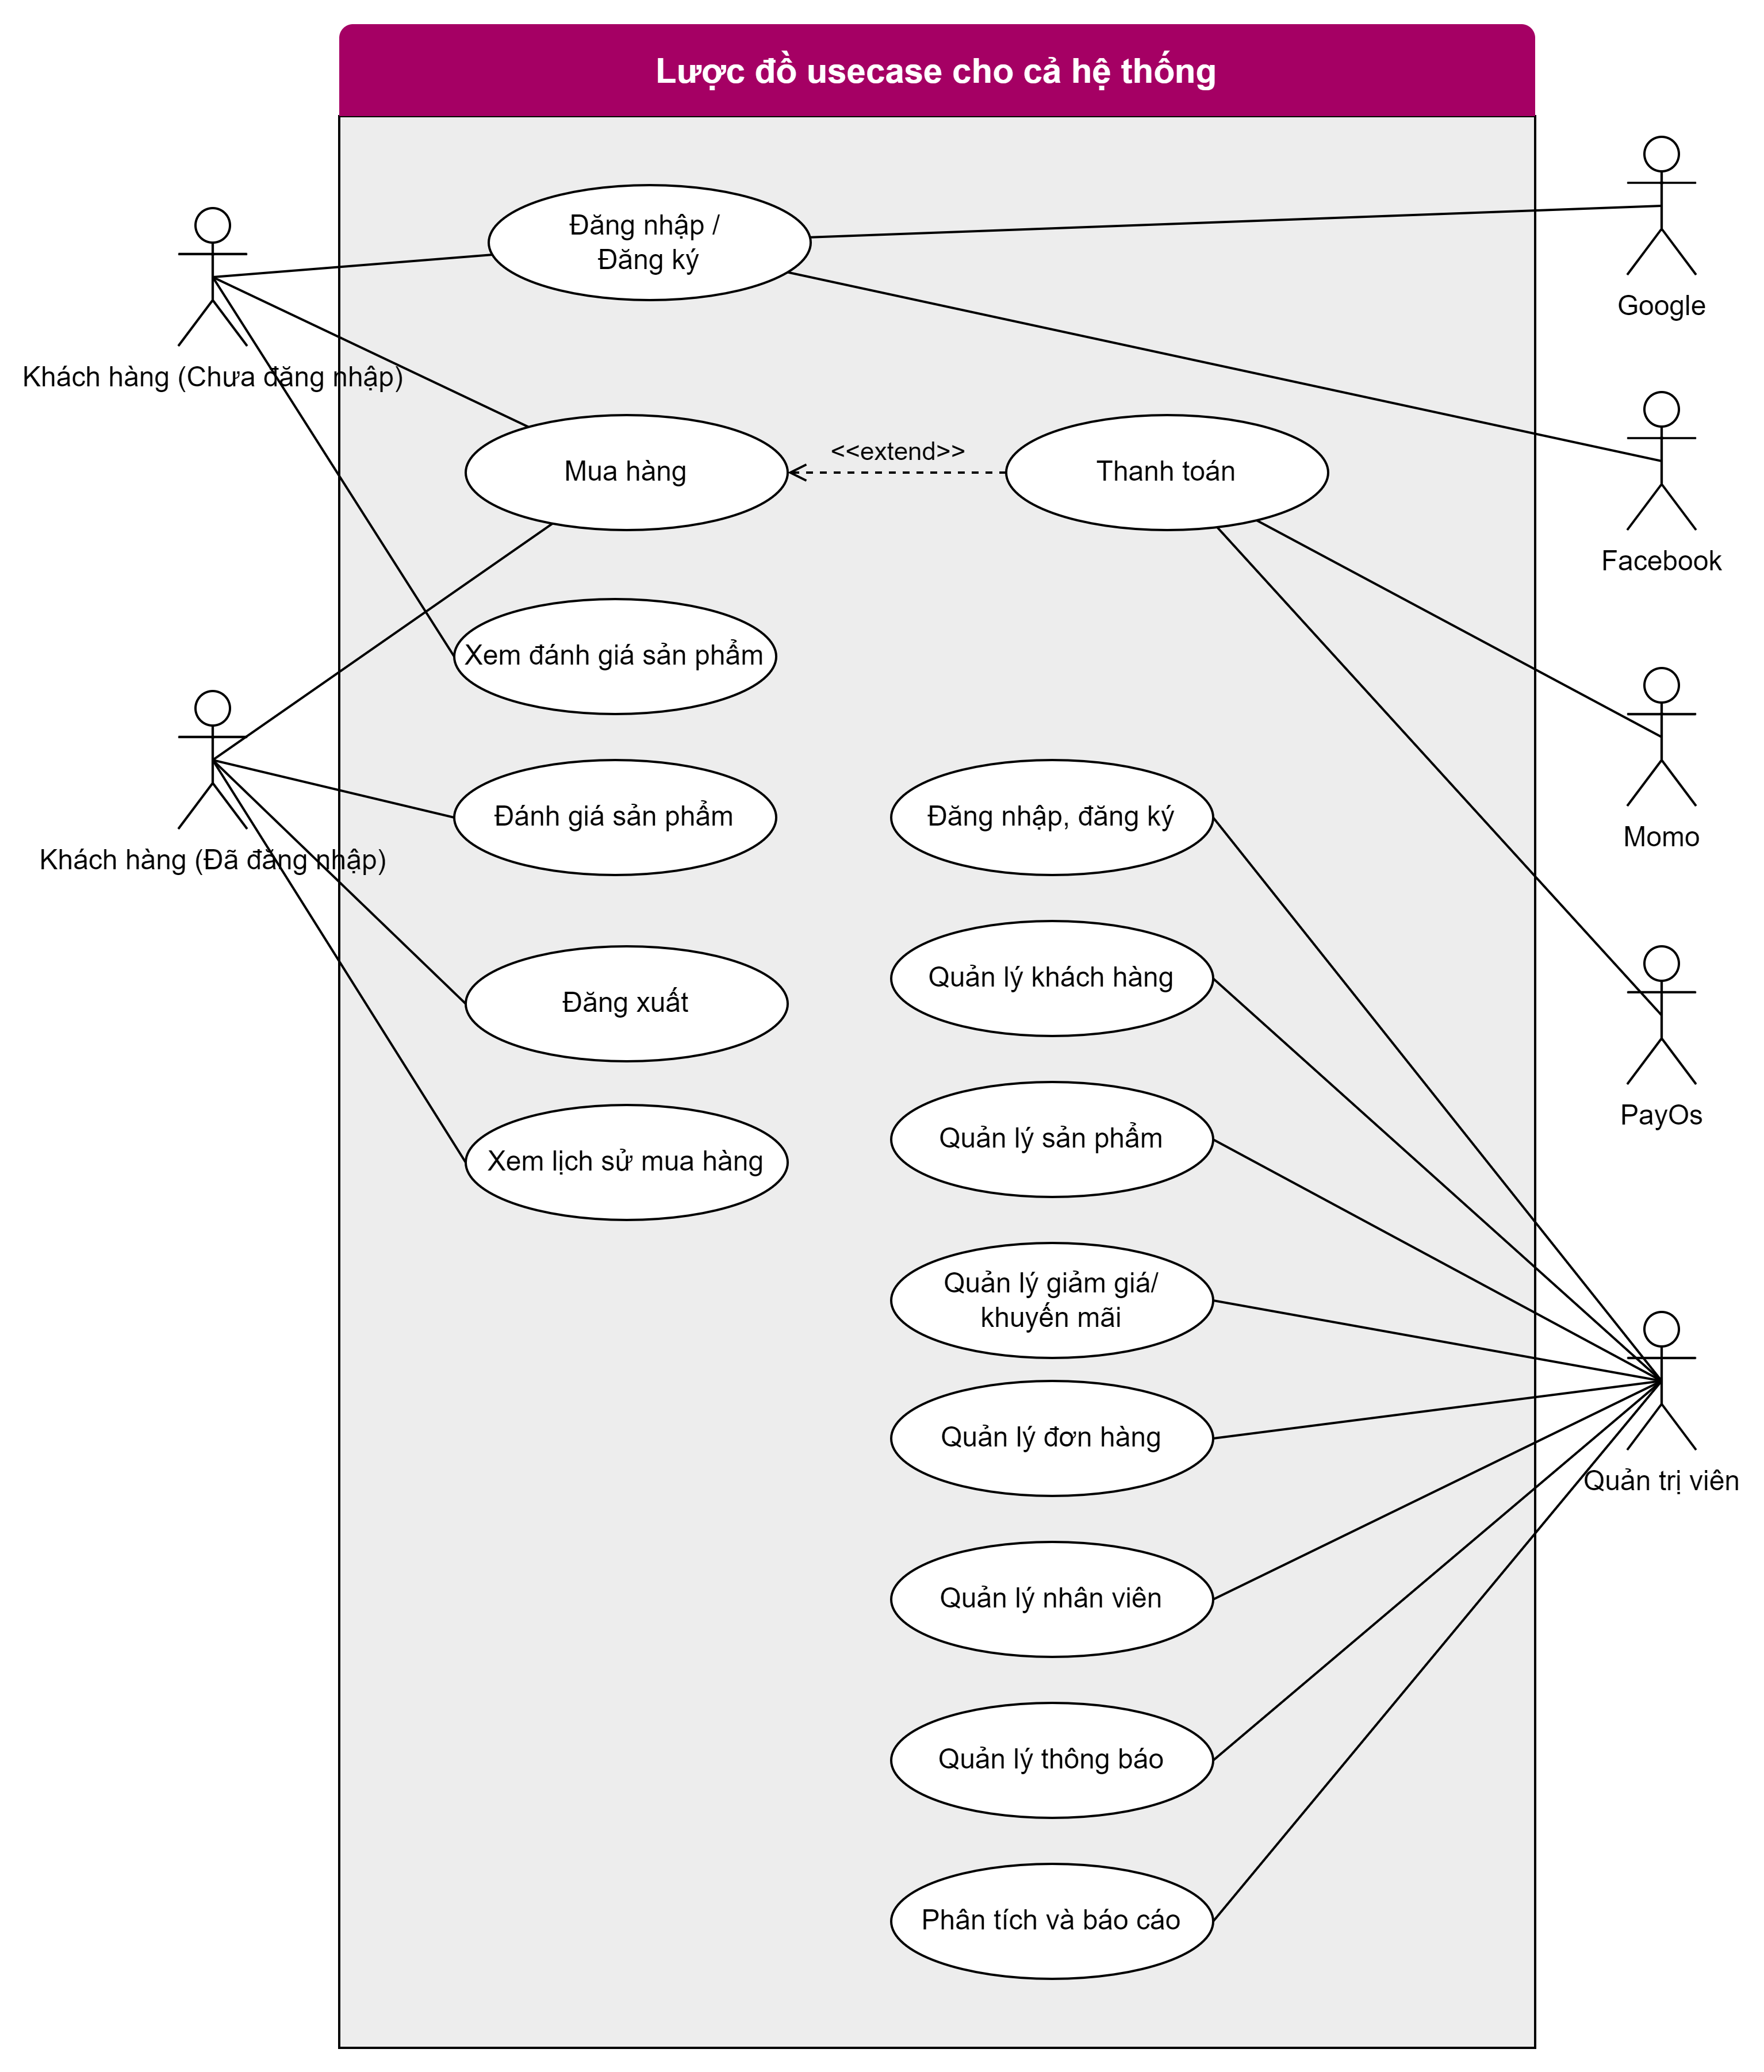
\includegraphics[width=14cm]{Images/usecase/OverallUsecase.png}
    \newline
    \caption{Sơ đồ Use-Case cho toàn bộ hệ thống}
    \label{fig:enter-label}
\end{figure}

\newpage
\subsection{Sơ đồ usecase chi tiết}
\subsubsection{Đăng nhập, đăng ký}
\begin{enumerate}[a.]
    \item \textbf{Use-case diagram}
        \begin{figure}[H]
            \centering
            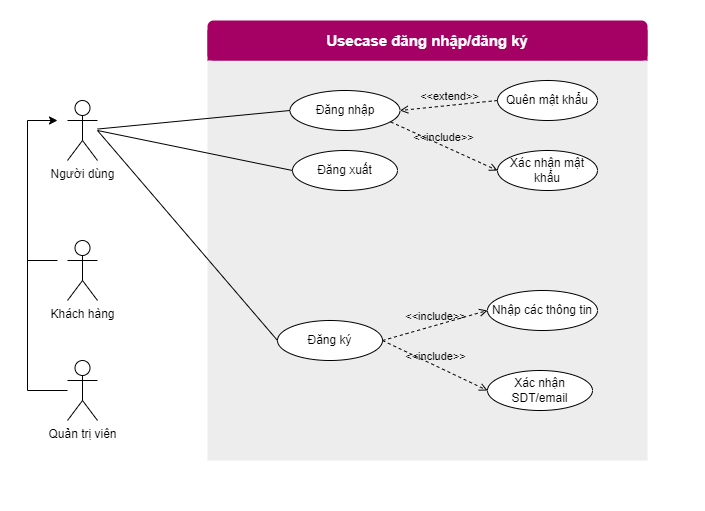
\includegraphics[width=15cm]{Images/usecase/Login-usecase.png}
            \caption{Use case diagram cho đăng nhập và đăng ký}
        \end{figure}
        
    \begin{longtable}{|p{3.5cm}|p{11.5cm}|}
        \hline
        Name &
          Đăng nhập \\ \hline
        Actor(s) &
          Người dùng \\ \hline
        Description &
          Cho phép người dùng đăng nhập vào hệ thống \\ \hline
        Trigger &
          Người dùng chọn nút "Đăng nhập" tại trang giao diện chính của hệ thống\\ \hline
        Pre-condition(s) & \begin{tabular}{@{}p{\linewidth}}
            - Người dùng chưa đăng nhập vào hệ thống\\
            - Người dùng có tài khoản để đăng nhập\\
            - Thiết bị của người dùng phải có kết nối internet ổn định
        \end{tabular} \\ 
          \hline
        Post-condition(s) & Người dùng đăng nhập thành công vào hệ thống.\\ 
        \hline
        Main Flow &
          \begin{tabular}[c]{@{}p{\linewidth}}
            1. Người dùng chọn "Đăng nhập" \\
            2. Hệ thống chuyển đến trang đăng nhập \\
            3. Người dùng nhập số điện thoại/email và mật khẩu \\
            4. Người dùng nhấn nút "Đăng nhập" \\
            5. Hệ thống kiểm tra số điện thoại/email và mật khẩu \\
            6. Hệ thống cập nhật lại giao diện người dùng tùy theo thông tin tài khoản.
        \end{tabular} \\ 
        \hline
        Alternative Flow &
        \begin{tabular}[c]{@{}p{\linewidth}} 
          \textbf{A1: Tại bước 2.}\\
           2.1: Người dùng nhấn vào "Quên mật khẩu" \\
           2.2: Hệ thống cung cấp phương pháp đặt lại mật khẩu của tài khoản\\
        Tiếp tục bước 3 trong Main Flow \\
            \textbf{A2: Tại bước 2.} \\
            2.1. Người dùng nhấn vào "Đăng ký tài khoản"\\
            2.2. Hệ thống chuyển đến trang đăng ký tài khoản \\
        Tiếp tục bước 2 trong Main Flow\\
        \end{tabular} \\ 
        \hline
        Exception & 
        \begin{tabular}[c]{@{}p{\linewidth}} 
          \textbf{E1: Tại bước 5.}\\
           5.1: Người dùng nhập sai số điện thoại/email hoặc mật khẩu\\
           5.2:  Hệ thống hiển thị thông tin đăng nhập sai \\
          Quay lại bước 2 trong Main Flow.\\
        \end{tabular} \\ \hline
        \caption{Use-case đăng nhập}
    \end{longtable}
    
    \newpage
    
    \begin{longtable}{|p{3.5cm}|p{11.5cm}|}
        \hline
        Name & Đăng ký \\ 
        \hline
        Actor(s) & Người dùng  \\ 
        \hline
        Description & Cho phép người dùng đăng ký trở thành thành viên \\ 
        \hline
        Trigger & Người dùng chọn "Đăng kí tài khoản" tại trang đăng ký\\ 
        \hline
        Pre-condition(s) & \begin{tabular}[c]{@{}p{\linewidth}}
            - Người dùng có số điện thoại chưa đăng kí tài khoản trên ứng dụng\\
            - Thiết bị của người dùng phải có kết nối internet ổn định
        \end{tabular} \\
        \hline
        Post-condition(s) & Người dùng tạo thành công tài khoản thành viên trên website và đăng nhập thành công vào hệ thống\\ 
        \hline
        Main Flow &
          \begin{tabular}[c]{@{}p{\linewidth}}
            1. Người dùng nhấn vào "Đăng ký tài khoản"\\
            2. Hệ thống chuyển sang giao diện yêu cầu người dùng nhập số điện thoại.\\
            3. Người dùng nhập số điện thoại vào và nhấn "Xác nhận".\\
            4. Hệ thống chuyển sang giao diện yêu cầu người dùng nhập các thông tin bao gồm tên đăng nhập, mật khẩu, xác nhận mật khẩu\\
            5. Người dùng điền đầy đủ thông tin được yêu cầu ở bước 4\\
            6. Người dùng chọn "Đăng ký"\\
            7. Đăng ký thành công và chuyển sang giao diện trang chủ\\
        \end{tabular} \\ 
        \hline
        Alternative Flow &
          \begin{tabular}[c]{@{}p{\linewidth}} 
            \textbf{A1: tại bước 2}\\
            2.1. Nếu người dùng đã có tài khoản, nhấn "Đăng nhập"\\
            2.2. Hệ thống chuyển sang trang đăng nhập\\
            \textbf{A2: tại bước 5}\\
            Người dùng muốn nhập lại số điện thoại khác thì nhấn "Quay lại", tiếp tục bước 2 trong Main Flow\\
        \end{tabular} \\ 
        \hline
        Exception & \begin{tabular}[c]{@{}p{\linewidth}} 
          \textbf{E1: Tại bước 3}\\
            3.1 Số điện thoại người dùng nhập vào không hợp lệ, hệ thống hiển thị thông báo lỗi\\
            Quay lại bước 2 trong Main flow\\
          \textbf{E2: Tại bước 3:}\\
            3.1. Số điện thoại người dùng nhập vào đã được đăng ký trên hệ thống, giao diện hiển thị thông báo "Số điện thoại này đã được đăng ký"\\
            Quay lại bước 2 trong Main Flow\\
            \textbf{E3: tại bước 5}\\
            5.1: Thông tin người dùng nhập vào không hợp lệ, hệ thống hiển thị thông báo lỗi tương ứng và yêu cầu người dùng nhập lại.\\
            Quay lại bước 4 trong Main Flow
        \end{tabular} \\ 
        \hline
        \caption{Use-case đăng ký}
    \end{longtable}
\end{enumerate}

\newpage
\subsubsection{Chức năng đặt hàng sản phẩm}
\begin{enumerate}[a. ]
    \item \textbf{Use-case diagram}
        \begin{figure}[h]
            \centering
            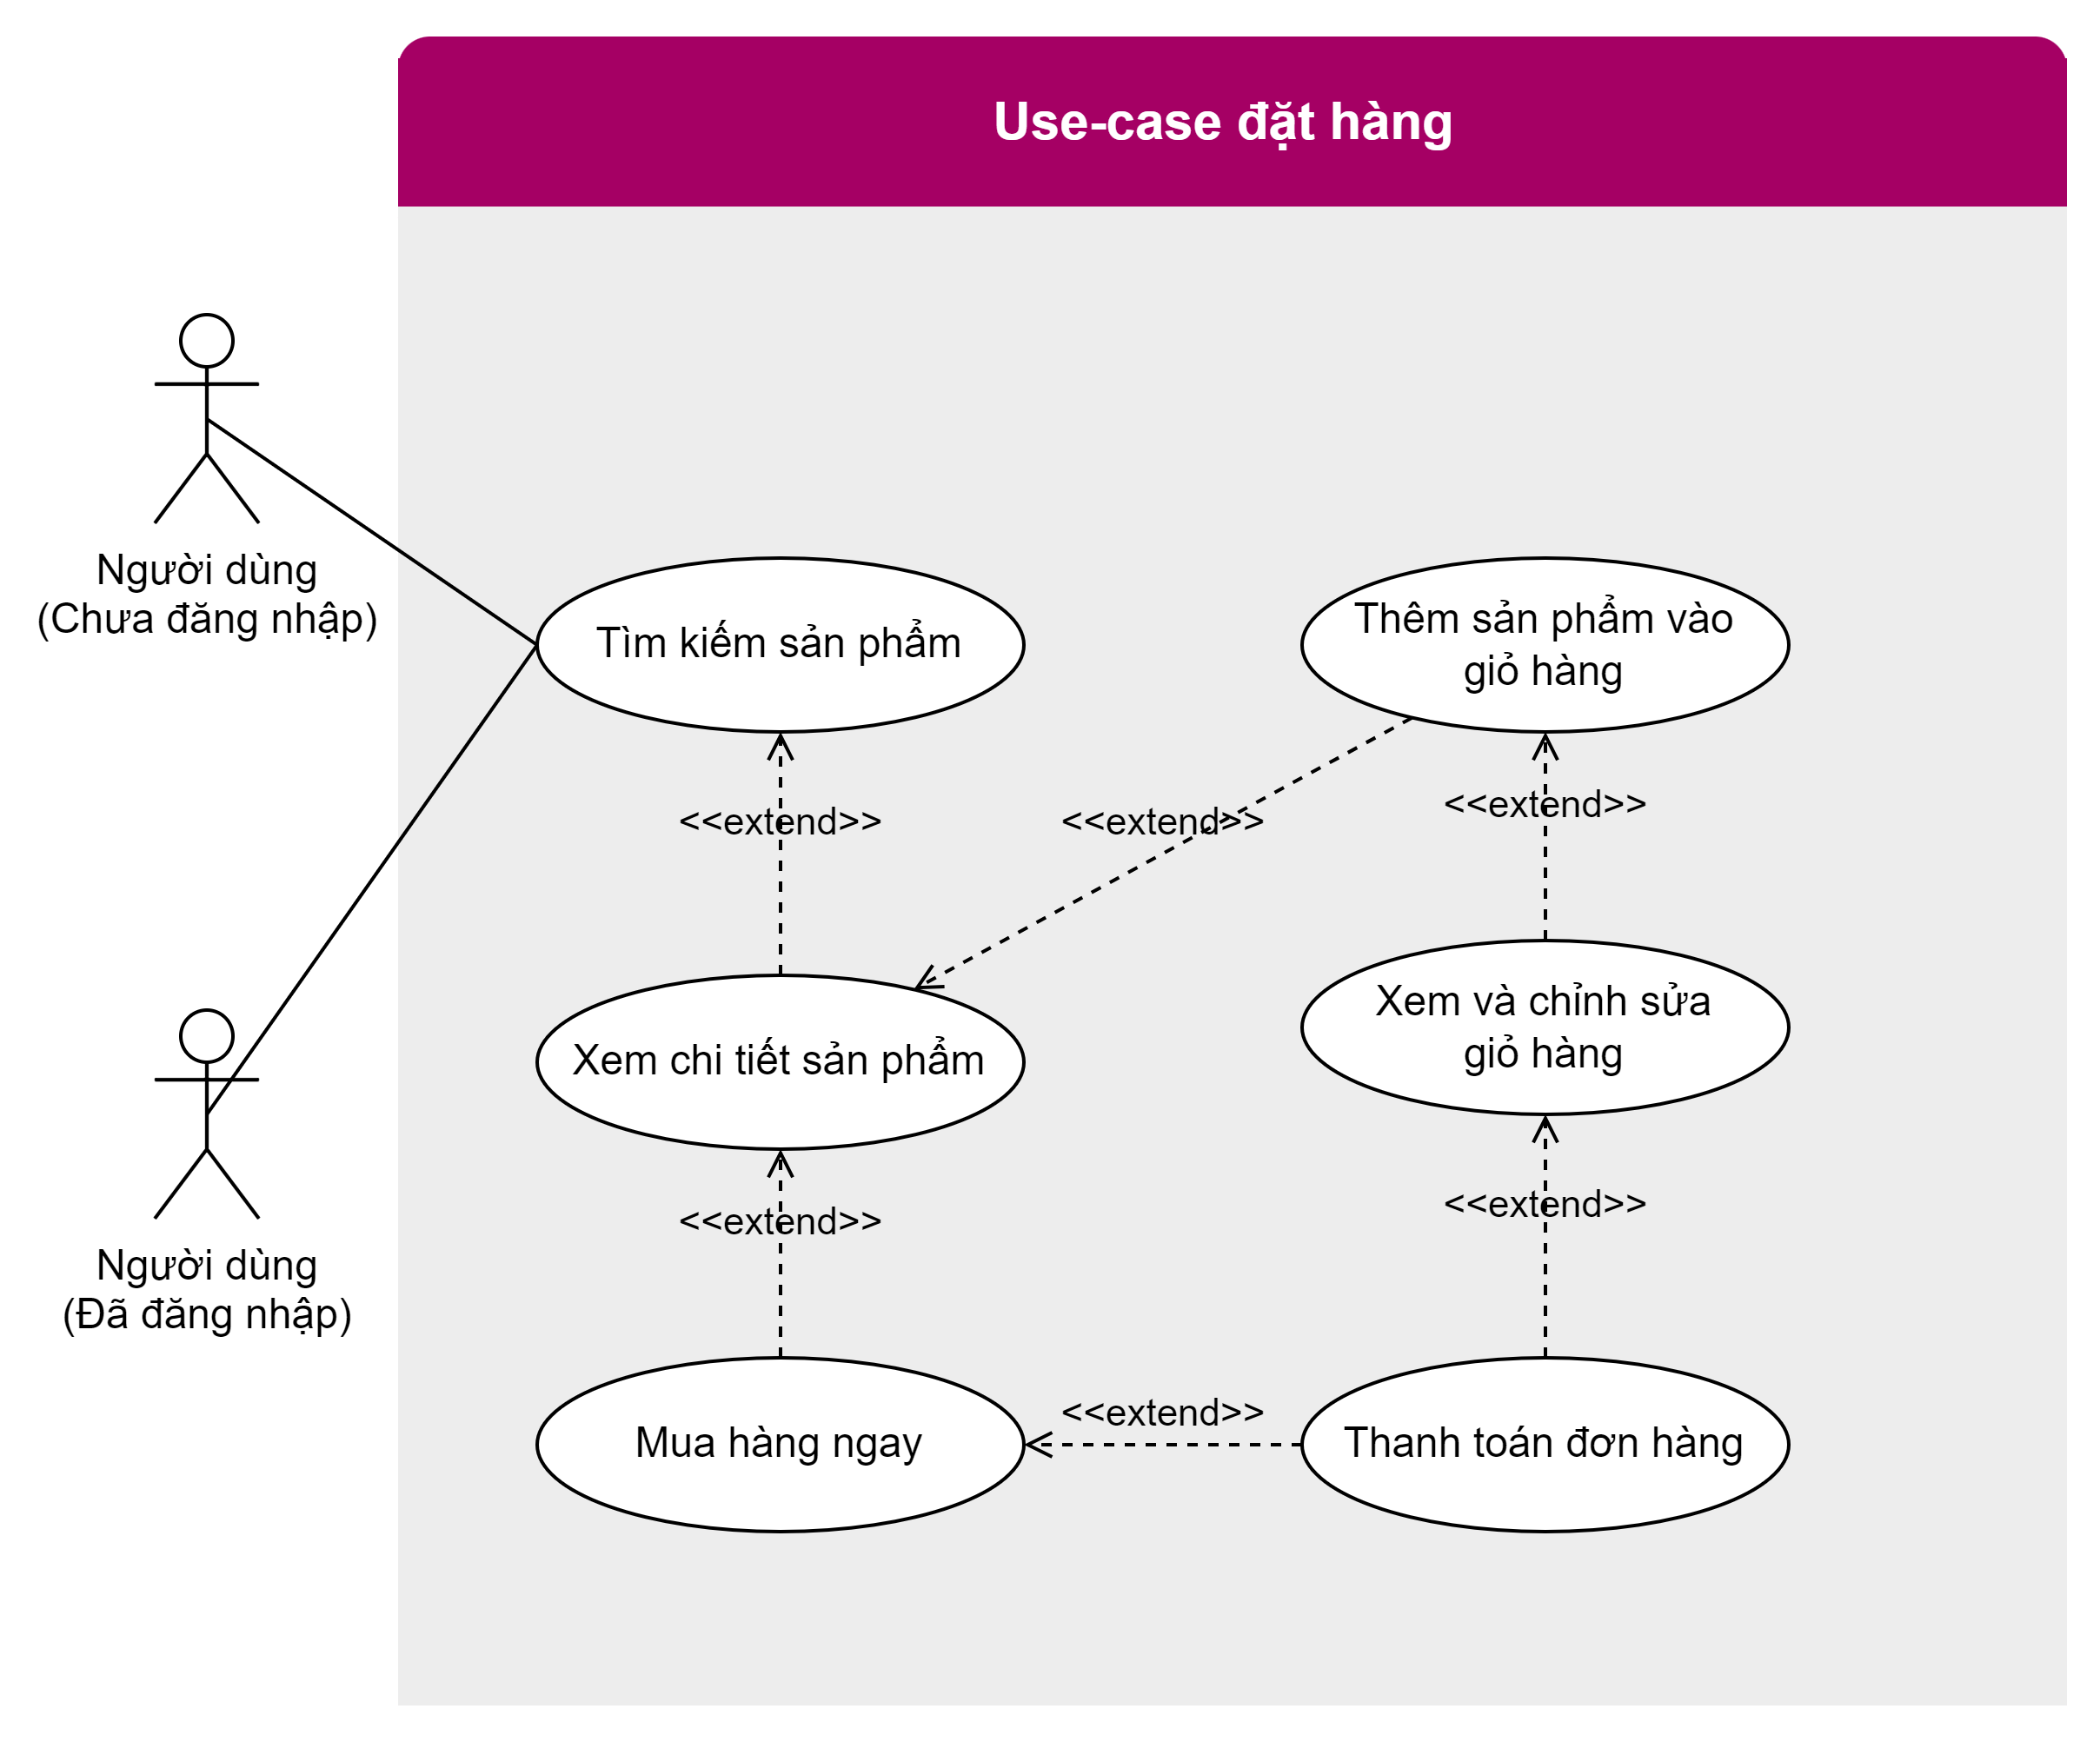
\includegraphics[width=15cm]{Images/usecase/orderUsecase.png}
            \newline
            \caption{Use-case diagram cho đặt hàng sản phẩm}
            \label{fig:enter-label}
        \end{figure}
    \newpage
    
    \item \textbf{Mô tả use-case}
    \begin{longtable}{|p{3.5cm}|p{11.5cm}|}
        \hline
        Name & Tìm kiếm sản phẩm \\ \hline
        Actor(s) &
          Tất cả người dùng \\ \hline
        Description &
          Cho phép người dùng tìm kiếm một mặt hàng cụ thể trên ứng dụng cửa hàng thời trang trực tuyến \\ 
        \hline
        Trigger &
          Người dùng muốn tìm kiếm một sản phẩm nào đó\\ \hline
        Pre-condition(s) & \begin{tabular}[c]{@{}p{\linewidth}}
            - Người dùng phải ở trang chủ của ứng dụng\\
        \end{tabular} \\ 
        \hline
        Post-condition(s) & Người dùng đã tìm được sản phẩm cần mua trong ứng dụng\\ 
        \hline
        Main Flow &
          \begin{tabular}[c]{@{}p{\linewidth}}
            1. Người dùng nhấn vào thanh tìm kiếm trên cùng của ứng dụng \\
            2. Hệ thống chuyển sang giao diện yêu cầu người dùng nhập thông tin cần tìm kiếm\\
            3. Người dùng nhập thông tin tìm kiếm và bấm "OK" ở bàn phím hoặc bấm vào biểu tượng hình kính lúp bên cạnh ô tìm kiếm\\
            4. Hệ thống hiển thị những sản phẩm mà người dùng đã tìm kiếm.
        \end{tabular} \\ 
        \hline
        Alternative Flow &
          \begin{tabular}[c]{@{}p{\linewidth}} 
          \textbf{A1: Tại bước 3.}\\
           3.1. Người dùng bấm "Hủy" trên bàn phím hoặc biểu tượng "x" trên thanh tìm kiếm.\\
           3.2. Hệ thống đưa người dùng về lại trang chủ \\
        \end{tabular} \\ 
        \hline
        Exception & \begin{tabular}[c]{@{}p{\linewidth}} 
          \textbf{ E1: Tại bước 4.}\\
           5.1. Nếu không có sản phẩm được tìm thấy thì hiển thị "Không tìm thấy sản phẩm". \\
          \textbf{ E2: Tại bước 4.}\\
           5.2. Nếu hệ thống có vấn đề thì phải thông báo đến người dùng. \\
        \end{tabular} \\ \hline
    \caption{Use-case tìm kiếm sản phẩm}
    \end{longtable}
    
    \newpage

    \begin{longtable}{|p{3.5cm}|p{11.5cm}|}
        \hline
        Name & Thêm sản phẩm vào giỏ hàng \\ \hline
        Actor(s) &
          Tất cả người dùng \\ \hline
        Description &
          Cho phép người dùng thêm một sản phẩm muốn mua vào giỏ hàng khi người dùng muốn mua nhiều sản phẩm \\ \hline
        Trigger &
          Người dùng muốn mua một sản phẩm nào đó\\ \hline
        Pre-condition(s) & Người dùng phải ở trang thông tin chi tiết của sản phẩm\\
          \hline
        Post-condition(s) & Người dùng đã thêm được sản phẩm cần mua vào trong giỏ hàng\\ \hline
        Main Flow &
          \begin{tabular}[c]{@{}p{\linewidth}}
            1. Người dùng nhấn vào nút "Thêm vào giỏ hàng". \\
            2. Nếu người dùng chưa chọn kích thước hoặc màu sẽ hiển thị lên kích thước và màu để nguời dùng chọn.\\
            3. Sau khi người dùng chọn xong thì bấm "Xác nhận".\\
            4. Hệ thống thêm sản phẩm người dùng chọn vào giỏ hàng.
        \end{tabular} \\ \hline
        Alternative Flow &
          \begin{tabular}[c]{@{}p{\linewidth}} 
          \textbf{A1: Tại bước 3.}\\
           3.1. Người dùng bấm "Hủy" chọn kích thước và màu.\\
           3.2. Hệ thống đưa người dùng về lại trang thông tin sản phẩm \\
        \end{tabular} \\ \hline
          
        Exception & None \\
        \hline
    \caption{Use-case thêm sản phẩm vào giỏ hàng}
    \end{longtable}

    \newpage
    \begin{longtable}{|p{3.5cm}|p{11.5cm}|}
        \hline
        Name & Sửa đổi số lượng sản phẩm trong giỏ hàng \\ \hline
        Actor(s) &
          Tất cả người dùng \\ \hline
        Description &
          Cho phép người dùng thay đổi số lượng sản phẩm muốn mua trong giỏ hàng. \\ \hline
        Trigger &
          Người dùng muốn sửa đổi số lượng sản phẩm trong giỏ hàng.\\ \hline
        Pre-condition(s) & Người dùng phải ở trang giỏ hàng.\\
          \hline
        Post-condition(s) & Người dùng đã sửa số lượng sản phẩm trong giỏ hàng thành công\\ \hline
        Main Flow &
        \begin{tabular}[c]{@{}p{\linewidth}}
            1. Người dùng cần xác định sản phẩm muốn thay đổi số lượng. \\
            2. Người dùng nhấn vào nút "+" để tăng số lượng hoặc "-" để giảm số lượng sản phẩm.\\
            3. Hệ thống tính toán lại giá tiền sản phẩm.\\
        \end{tabular} \\ 
        \hline
        Alternative Flow & None \\
        \hline
        Exception & None \\
        \hline
    \caption{Use-case sửa số lượng sản phẩm trong giỏ hàng}
    \end{longtable}
    
    \newpage
    
    \begin{longtable}{|p{3.5cm}|p{11.5cm}|}
        \hline
        Name & Xóa sản phẩm ra khỏi giỏ hàng \\ \hline
        Actor(s) &
          Tất cả người dùng \\ 
          \hline
        Description &
          Cho phép người dùng xóa một sản phẩm ra khỏi giỏ hàng \\ 
          \hline
        Trigger &
          Người dùng không muốn mua sản phẩm đó nữa và muốn bỏ nó ra giỏ hàng\\ 
          \hline
        Pre-condition(s) & Người dùng phải ở trang giỏ hàng.\\
          \hline
        Post-condition(s) & Người dùng đã xóa sản phẩm ra khỏi giỏ hàng thành công\\ 
        \hline
        Main Flow &
          \begin{tabular}[c]{@{}p{\linewidth}}
            1. Người dùng cần xác định sản phẩm cần xóa ra khỏi giỏ hàng. \\
            2. Người dùng nhấn biểu tượng xóa.\\
            3. Hệ thống hiển thị một thông báo đến người dùng và yêu cầu nhấn vào nút "Xác nhận".\\
            4. Hệ thống xóa sản phẩm ra khỏi giỏ hàng.
        \end{tabular} \\ \hline
        Alternative Flow &
          \begin{tabular}[c]{@{}p{\linewidth}} 
          \textbf{A1: Tại bước 3.}\\
           3.1. Người dùng bấm "Hủy" xóa sản phẩm.\\
           3.2. Hệ thống tắt thông báo. \\
        \end{tabular} \\ \hline
        Exception & None \\
        \hline
    \caption{Use-case xóa sản phẩm ra khỏi giỏ hàng}
    \end{longtable}
    
    \newpage
    \begin{longtable}{|p{3.5cm}|p{11.5cm}|} 
        \hline
        Name & Người dùng muốn đặt mua sản phẩm \\ \hline
        Actor(s) &
          Tất cả người dùng \\ 
          \hline
        Description &
          Cho phép người dùng đặt đơn sản phẩm \\ 
          \hline
        Trigger &
          Người dùng muốn mua sản phẩm\\ 
          \hline
        Pre-condition(s) & \begin{tabular}[c]{@{}p{\linewidth}}
            - Người dùng phải ở trang giỏ hàng và tích vào những sản phẩm cần mua. \\
            - Người dùng đang ở trang chi tiết sản phẩm và bấm "Mua ngay".\\
        \end{tabular} \\ 
        \hline
        Post-condition(s) & Người dùng đã đặt hàng thành công và chuyển sang phương thức thanh toán\\ 
        \hline
        Main Flow &
          \begin{tabular}[c]{@{}p{\linewidth}}
            1. Người dùng cần xác định sản phẩm cần mua ở trong giỏ hàng hoặc ở trang chi tiết sản phẩm cần mua . \\
            2. Người dùng nhấn nút "Mua ngay".\\
            3. Hệ thống đưa người dùng đến trang xác nhận đơn hàng.\\
            4. Người dùng xác nhận địa chỉ nhận hàng.\\
            5. Người dùng nhập hoặc áp mã giảm giá (nếu có).\\
            6. Hệ thống kiểm tra mã giảm giá có hợp lệ.\\
            7. Hệ thống tính tổng tiền cho đơn hàng.
        \end{tabular} \\ \hline
        Alternative Flow &
          \begin{tabular}[c]{@{}p{\linewidth}} 
          \textbf{A1: Tại bước 4: Người dùng chưa đăng nhập}\\
           4.1. Người dùng điền tên, số điện thoại và địa chỉ.\\
           4.2. Tiếp tục bước 5. \\
        \end{tabular} \\ \hline
        Exception & None \\
        \hline
        \caption{Use-case đặt hàng}
    \end{longtable}
\end{enumerate}
\newpage

\subsubsection{Phương thức thanh toán}
\begin{enumerate}[a. ]
    \item \textbf{Use-case Diagram}
        \begin{figure}[h]
            \centering
            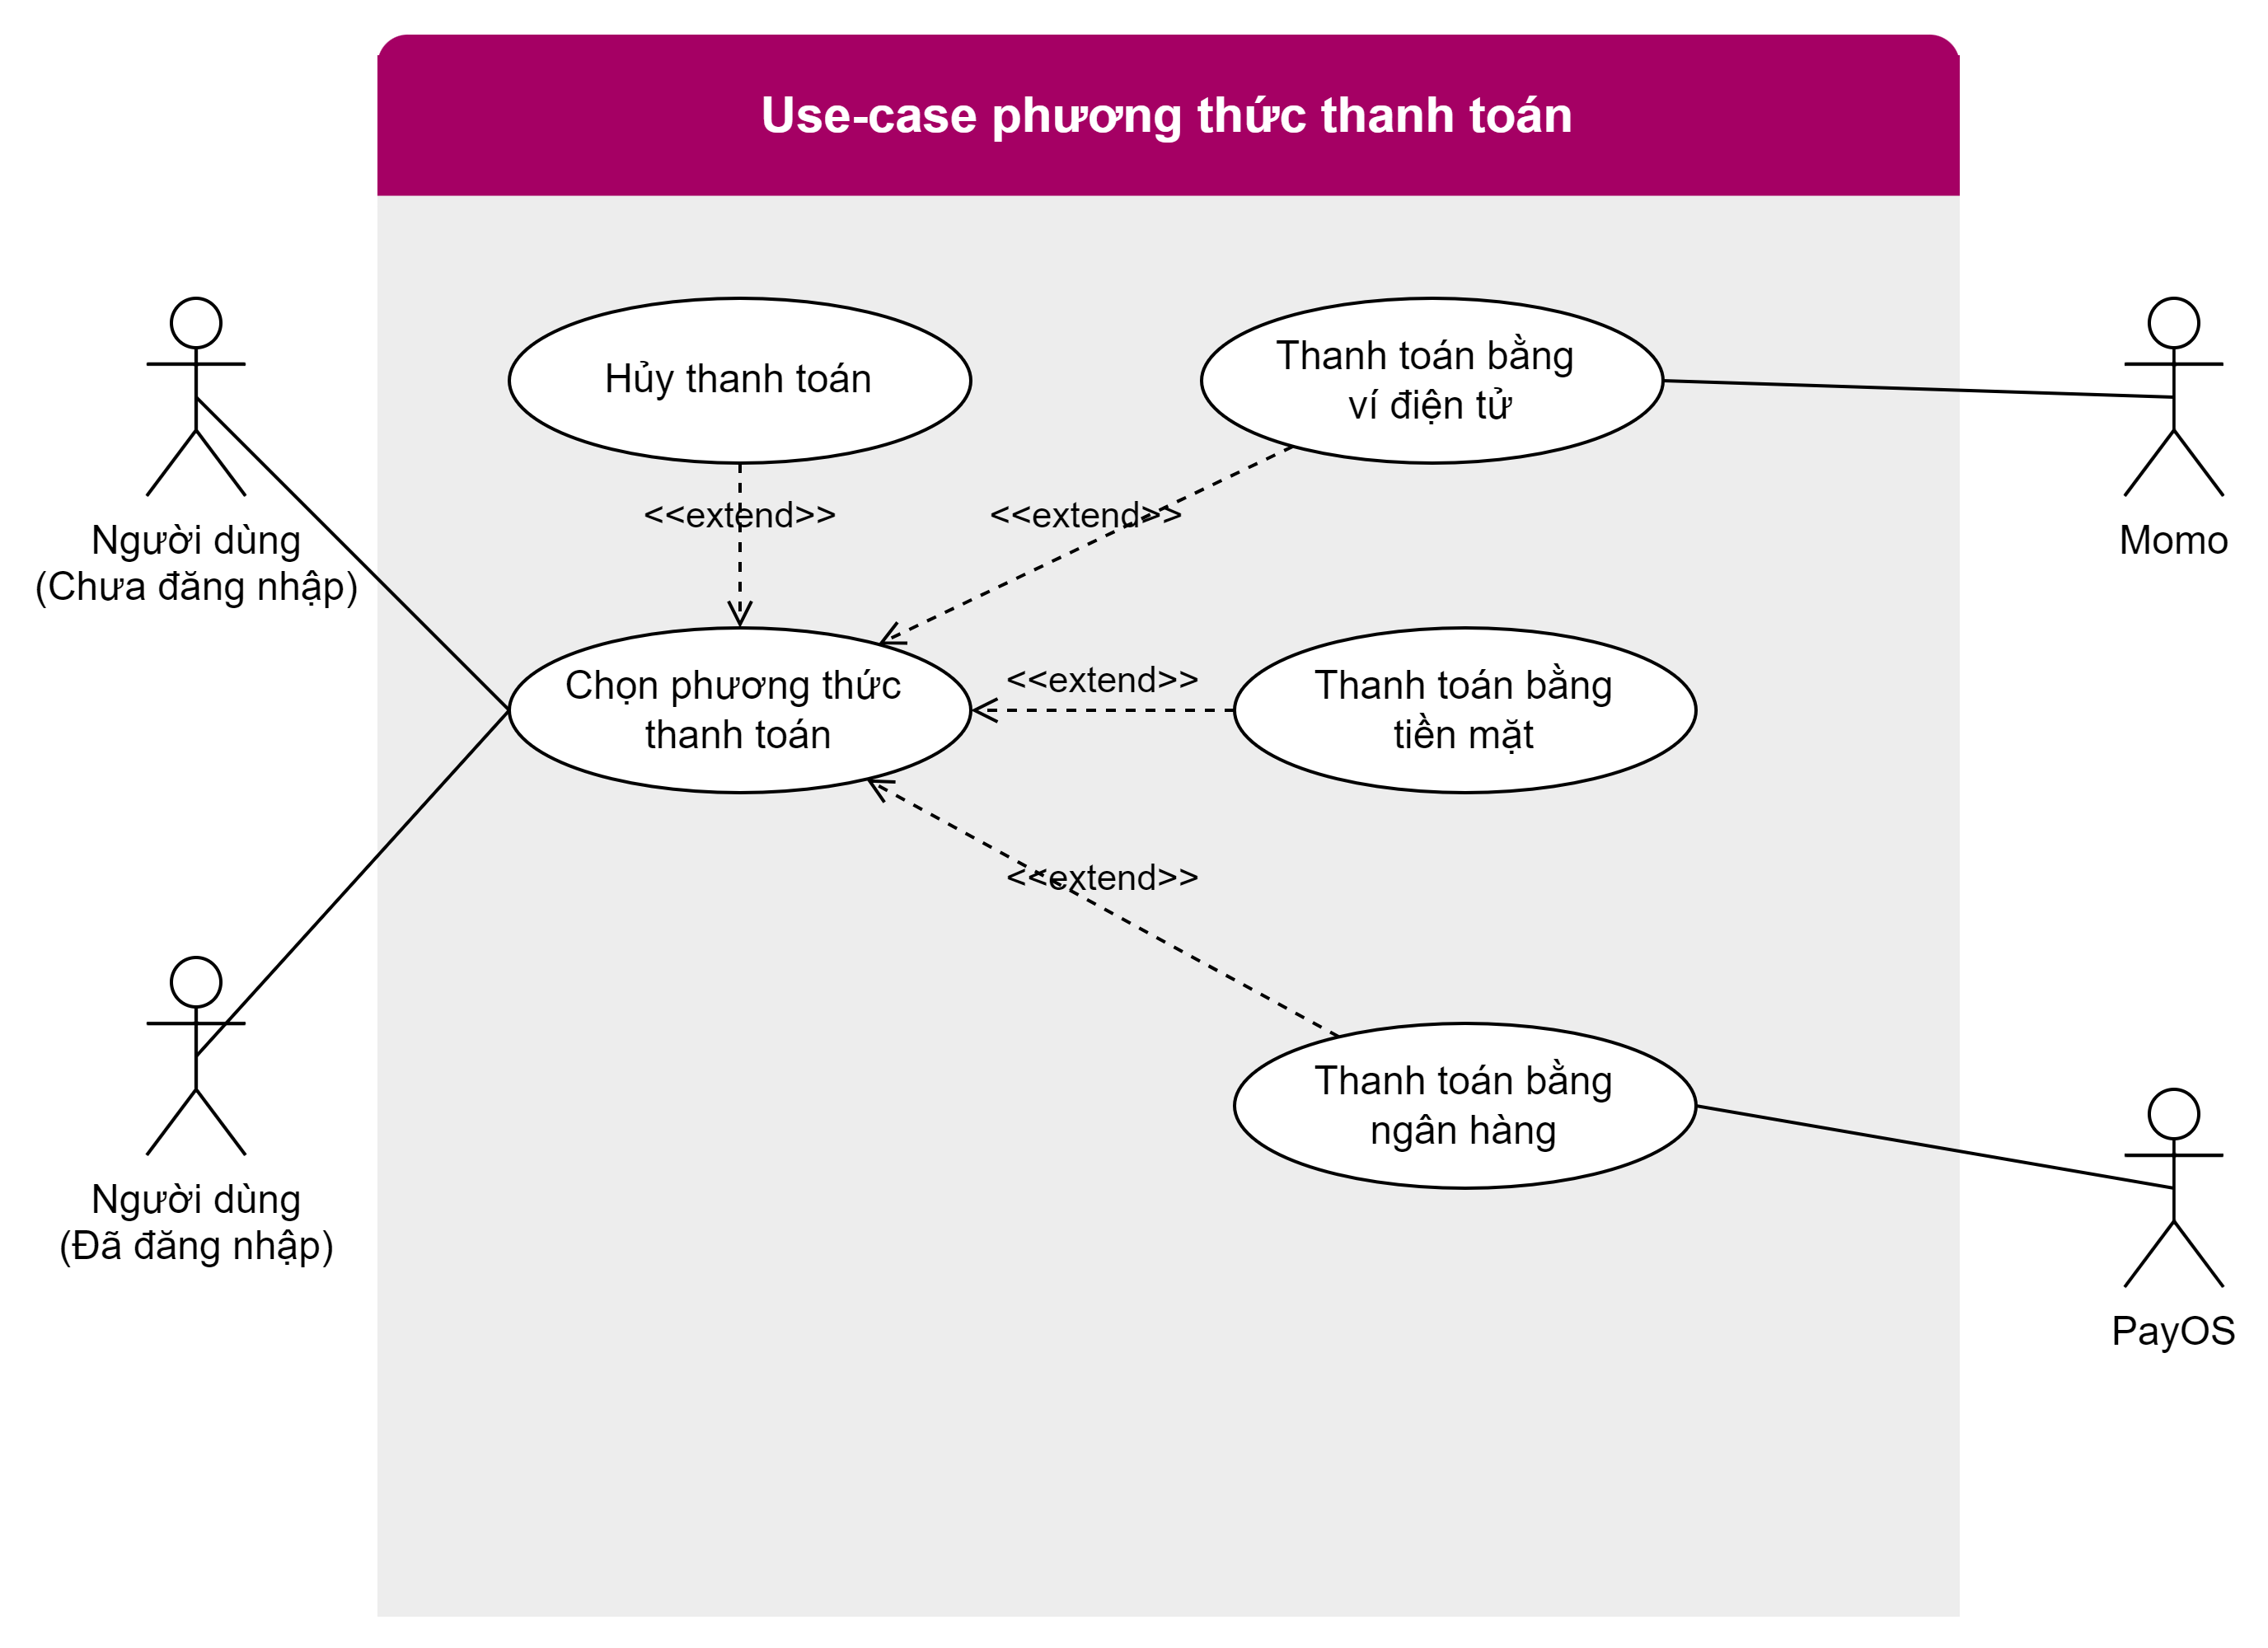
\includegraphics[width=15cm]{Images//usecase/UseCasePaymentMomo.png}
            \newline
            \caption{Use-case diagram cho phương thức thanh toán}
            \label{fig:enter-label}
        \end{figure}
    \newpage
    \item \textbf{Mô tả use-case}
    
    \begin{longtable}{|p{3.5cm}|p{11.5cm}|}  
        \hline
        Name & Thanh toán bằng ví Momo \\ \hline
        Actor(s) &
          Tất cả người dùng \\ 
          \hline
        Description &
          Cho phép người dùng thanh toán đơn hàng bằng ví điện tử \\ 
          \hline
        Trigger &
          Người dùng muốn mua thanh toán sản phẩm bằng Momo\\ 
          \hline
        Pre-condition(s) & \begin{tabular}[c]{@{}p{\linewidth}}
            - Người dùng phải ở trang chọn phương thức thanh toán. \\
            - Người dùng phải có và cài đặt ứng dụng Momo.\\
        \end{tabular} \\ 
        \hline
        Post-condition(s) & Người dùng thanh toán thành công đơn hàng\\ 
        \hline
        Main Flow &
          \begin{tabular}[c]{@{}p{\linewidth}}
            1. Người dùng chọn phương thức thanh toán Momo . \\
            2. Người dùng nhấn nút "Điều hướng sang ứng dụng Momo".\\
            3. Hệ thống đưa người dùng đến ứng dụng Momo.\\
            4. Người dùng thực hiện chuyển tiền.\\
            5. Ứng dụng Momo chuyển về lại ứng dụng cửa hàng.\\
            6. Hệ thống hiển thị thông tin đơn hàng được thanh toán thành công.\\
        \end{tabular} \\ \hline
        Alternative Flow &
          \begin{tabular}[c]{@{}p{\linewidth}} 
          \textbf{A1: Tại bước 2: Người dùng thực hiện thanh toán bằng mã QR}\\
           2.1. Người dùng quét mã thanh toán bằng điện thoại khác hoặc lưu mã QR.\\
           2.2. Hệ thống kiểm tra đơn hàng đã được thanh toán chưa. \\
           2.3. Tiếp tục bước 6.
        \end{tabular} \\ \hline
        Exception & \begin{tabular}[c]{@{}p{\linewidth}}
            \textbf{E1: Tại bước 2: người dùng không có ứng dụng Momo}\\
            Không thể chuyển sang ứng dụng Momo được.
        \end{tabular}\\ 
        \hline
        \caption{Use-case thanh toán ví điện tử}
    \end{longtable}
    
    \newpage
    \begin{longtable}{|p{3.5cm}|p{11.5cm}|}
        \hline
        Name & Thanh toán bằng ngân hàng \\ \hline
        Actor(s) &
          Người dùng \\ \hline
        Description &
          Cho phép người dùng thanh toán đơn hàng bằng tài khoản ngân hàng. \\ \hline
        Trigger &
          Người dùng muốn thanh toán đơn hàng bằng tài khoản ngân hàng\\ \hline
        Pre-condition(s) & Người dùng phải ở trang chọn phương thức thanh toán.\\
          \hline
        Post-condition(s) & Người dùng thanh toán đơn hàng thành công.\\ \hline
        Main Flow &
        \begin{tabular}[c]{@{}p{\linewidth}}
           1. Người dùng chọn phương thức thanh toán bằng ngân hàng . \\
            2. Hệ thống điều hướng người dùng sang trình duyệt.\\
            3. Người dùng thực hiện quét mã QR để thanh toán.\\
            4. Hệ thống thứ 3 kiểm tra giao dịch thành công sẽ đẩy ngược về lại ứng dụng bán hàng.\\
            5. Hệ thống hiển thị thông tin đơn hàng được thanh toán thành công.\\
        \end{tabular} \\ 
        \hline
        Alternative Flow & None \\
        \hline
        Exception & None \\ 
        \hline
    \caption{Use-case thanh toán bằng ngân hàng}
    \end{longtable}
\end{enumerate}

\newpage

\subsubsection{Quản lý thông tin cá nhân}
\begin{enumerate}[a. ]
    \item \textbf{Use-case Diagram}
        \begin{figure}[H]
            \centering
            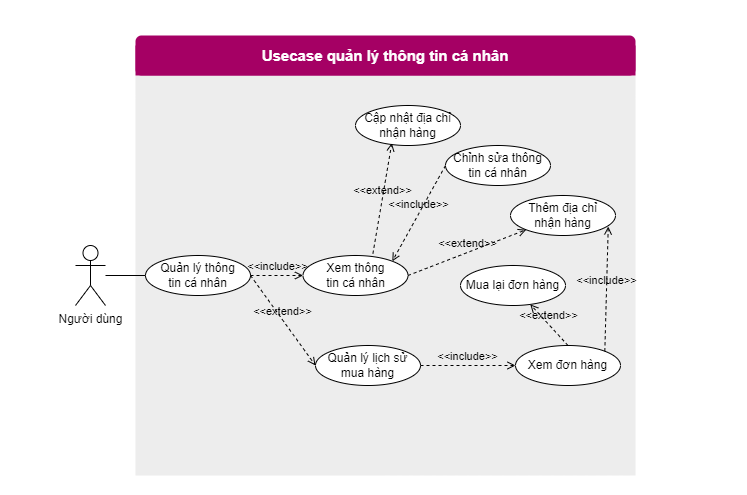
\includegraphics[width=17cm]{Images/usecase/ManageProfile.png}
            \newline
            \caption{Use-case diagram cho quản lý thông tin cá nhân}
        \end{figure}
    \newpage
    \item \textbf{Mô tả use-case}
    \begin{longtable}{|p{3.5cm}|p{11.5cm}|}
        \hline
        Name & Quản lý thông tin cá nhân \\ \hline
        Actor(s) &
          Người dùng \\ \hline
        Description &
          Cho phép người dùng xem, thay đổi thông tin cá nhân, xem lịch sử đơn hàng, thêm và cập nhật địa chỉ nhận hàng \\ \hline
        Trigger &
          Người dùng nhấn vào "Tài khoản của tôi"\\ \hline
        Pre-condition(s) & Người dùng đã đăng nhập tài khoản thành công.\\
          \hline
        Post-condition(s) & Người dùng thấy được thông tin cá nhân thành công\\ \hline
        Main Flow &
        \begin{tabular}[c]{@{}p{\linewidth}}
            1. Người dùng nhấn vào "Tài khoản của tôi" \\
            2. Hệ thống hiển thị thông tin cá nhân của người dùng\\
            3. Người dùng xem toàn bộ thông tin cá nhân\\
        \end{tabular} \\ 
        \hline
         Alternative Flow &
          \begin{tabular}[c]{@{}p{\linewidth}} 
          \textbf{A1: Tại bước 3.}\\
                  3.1: Người dùng chỉnh sửa thông tin cá nhân\\
        3.2: Hệ thống hiển thị màn hình để chỉnh sửa thông tin cá nhân\\
        3.3: Người dùng chỉnh sửa các thông tin cá nhân\\
        3.4 Người dùng nhấn cập nhật để thoát khỏi giao diện chỉnh sửa thông tin cá nhân. Hệ thống xác nhận chỉnh sửa thông tin cá nhân thành công.\\
\textbf{A2: Tại bước 3.}\\
        3.1: Người dùng nhấn vào nút "Xem lịch sử đơn hàng"\\
        3.2: Hệ thống hiển thị tất cả các đơn hàng đã mua\\

        \end{tabular} \\ \hline
        Exception & None \\
        \hline
    \caption{Use-case quản lý thông tin cá nhân}
    \end{longtable}
    
\end{enumerate}
\newpage
\subsubsection{Quản lý nhân viên}
\begin{enumerate}[a.]
    \item \textbf{Use-case diagram}
        \begin{figure}[H]
            \centering
            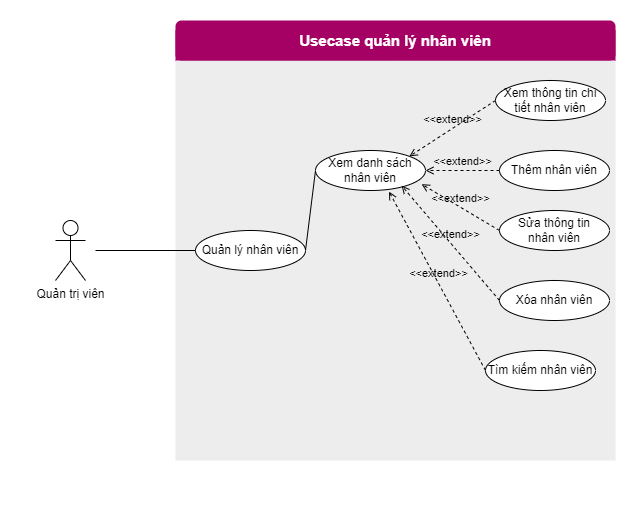
\includegraphics[width=16cm]{Images/usecase/ManageEmployee.png}
            \caption{Use case diagram cho quản lý nhân viên}
        \end{figure}
        
    \newpage
    \item \textbf{Mô tả usecase}
    \begin{longtable}{|p{3.5cm}|p{11.5cm}|}
        \hline
        Name &
          Xem thông tin chi tiết của nhân viên \\ \hline
        Actor(s) &
          Quản trị viên \\ \hline
        Description &
          Cho phép quản trị viên xem thông tin chi tiết của tất cả các nhân viên trên hệ thống \\ \hline
        Trigger &
          Quản trị viên chọn nút "Quản lý nhân viên" tại trang giao diện chính của hệ thống\\ \hline
        Pre-condition(s) & \begin{tabular}[c]{@{}p{\linewidth}}
- Quản trị viên đã đăng nhập vào hệ thống bằng tài khoản Manager\\
        \end{tabular} \\ 
          \hline
        Post-condition(s) &Quản trị viên xem được danh sách tất cả các nhân viên trong hệ thống.\\ \hline
        
        Main Flow &
          \begin{tabular}[c]{@{}p{\linewidth}}
            1 . Hệ thống hiển thị danh sách tất cả các nhân viên\\
        2 . Quản trị viên chọn cụ thể một nhân viên bằng cách nhấn vào nút icon xem chi tiết\\
        3 . Hệ thống hiển thị thông tin chi tiết của nhân viên\\
        \end{tabular} \\ 
        \hline
        Alternative Flow & \begin{tabular}[c]{@{}p{\linewidth}} 
            \textbf{A1: Tại bước 1: }\\
            1.1. Quản trị viên nhấn tìm kiếm tên 1 nhân viên cụ thể\\
            1.2.Hệ thống trả về các nhân viên thỏa mãn tiêu chí tìm kiếm \\
        \end{tabular} \\ 
        \hline
        Exception & None \\
        \hline
        \caption{Use-case xem thông tin chi tiết của nhân viên}
    \end{longtable}
    \newpage
    
    \begin{longtable}{|p{3.5cm}|p{11.5cm}|}        
        \hline
        Name &  Thêm nhân viên mới \\ \hline
        Actor(s) &
          Quản trị viên \\ \hline
        Description &
          Cho phép quản trị viên thêm một nhân viên mới\\ \hline
        Trigger &
          Quản trị viên nhấn vào thêm nhân viên\\ \hline
        Pre-condition(s) &
          \begin{tabular}[c]{@{}p{\linewidth}}
        Quản trị viên đã đăng nhập vào tài khoản của mình\\
        Quản trị viên đang trong màn hình quản lý nhân viên\\
        \end{tabular} \\ \hline
        Post-condition(s) & Quản trị viên thêm nhân viên thành công\\ \hline
        Main Flow &
          \begin{tabular}[c]{@{}p{\linewidth}}
        1 . Hệ thống chuyển sang giao diện nhập thông tin cho nhân viên mới\\
        2 . Quản trị viên nhập lần lượt các thông tin mà hệ thống yêu cầu (tên nhân viên, ngày sinh, địa chỉ, giới tính,...)\\
        3 . Quản trị viên nhấn "Xác nhận" để thoát khỏi giao diện thêm nhân viên\\
        4 . Hệ thống xác nhận thêm nhân viên thành công\\
        \end{tabular} \\ \hline
        Alternative Flow &
          None \\ \hline
        Exception & \begin{tabular}[c]{@{}p{\linewidth}} 
        \textbf{E1: Tại bước 3:}\\
        - Hệ thống hiển thị lỗi "Tên/địa chỉ/... không hợp lệ"\\
        - Hệ thống hiển thị lỗi "Không được để trống thông tin"\\
        \end{tabular} \\ \hline
        \caption{Use-case thêm nhân viên}
    \end{longtable}
    \newpage
    \begin{longtable}{|p{3.5cm}|p{11.5cm}|}
        \hline
        Name & Tìm kiếm nhân viên\\ \hline
        Actor(s) &
          Quản trị viên \\ \hline
        Description &
          Cho phép quản trị viên tìm kiếm nhân viên\\ \hline
        Trigger &
          \begin{tabular}[c]{@{}p{\linewidth}} 
        Quản trị viên nhấn vào ô tìm kiếm nhân viên\\
        
        \end{tabular} \\ \hline
        Pre-condition(s) & \begin{tabular}[c]{@{}p{\linewidth}} 
        Quản trị viên đã đăng nhập vào tài khoản của mình\\
        Quản trị viên đang trong màn hình quản lý nhân viên\\
        \end{tabular}\\
          \hline
        Post-condition(s) & Quản trị viên xem được thông tin nhân viên đã tìm kiếm\\ \hline
        Main Flow &
          \begin{tabular}[c]{@{}p{\linewidth}}
        1 . Quản trị viên nhập từ khóa tên của nhân viên cần tìm, rồi nhấn tìm kiếm\\
        2 . Hệ thống trả về danh sách tất cả nhân viên thỏa mãn yêu cầu của từ khóa \\
        \end{tabular} \\ \hline
        Alternative Flow & None
         \\ \hline
        Exception & \begin{tabular}[c]{@{}p{\linewidth}} 
        \textbf{E1: Tại bước 2:}\\
        - Hệ thống hiển thị lỗi "Không có nhân viên thỏa mãn yêu cầu"\\
        \end{tabular} \\ \hline
        \caption{Use-case tìm kiếm nhân viên}
    \end{longtable}
    \newpage
    \begin{longtable}{|p{3.5cm}|p{11.5cm}|}        
        \hline
        Name & Chỉnh sửa thông tin nhân viên\\ \hline
        Actor(s) &
          Quản trị viên \\ \hline
        Description &
          Cho phép quản trị viên thay đổi thông tin nhân viên trên hệ thống\\ \hline
        Trigger &
          Quản trị viên nhấn vào "Thay đổi thông tin nhân viên" \\ \hline
        Pre-condition(s) & \begin{tabular}[c]{@{}p{\linewidth}} 
        Quản trị viên đã đăng nhập vào tài khoản của mình\\
        Quản trị viên đang trong màn hình quản lý nhân viên\\
        Quản trị viên đã chọn được nhân viên cần thay đổi thông tin\\
        \end{tabular}\\
        \hline
        Post-condition(s) & Quản trị viên đã thay đổi thông tin thành công cho nhân viên\\ \hline
        Main Flow &
          \begin{tabular}[c]{@{}p{\linewidth}}
        1 . Hệ thống hiển thị 1 màn hình để chỉnh sửa các thông tin cần cho nhân viên\\
        2 . Quản trị viên chỉnh sửa lần lượt các thông tin của nhân viên\\
        3 . Quản trị viên nhấn "Cập nhật" để thoát khỏi giao diện chỉnh sửa thông tin nhân viên\\
        4 . Hệ thống xác nhận chỉnh sửa thông tin nhân viên thành công\\
        \end{tabular} \\ \hline
        Alternative Flow &
          None \\ \hline
        Exception & None \\ \hline
        \caption{Use-case chỉnh sửa thông tin nhân viên}
    \end{longtable}
    \newpage
    \begin{longtable}{|p{3.5cm}|p{11.5cm}|}
        \hline
        Name & Xóa nhân viên\\ \hline
        Actor(s) &
         Quản trị viên\\ \hline
        Description &
          Cho phép quản trị viên xóa nhân viên khỏi hệ thống\\ \hline
        Trigger &
          Quản trị viên nhấn vào "Xóa nhân viên" \\ \hline
        Pre-condition(s) & \begin{tabular}[c]{@{}p{\linewidth}} 
        Quản trị viên đã đăng nhập vào tài khoản của mình\\
        Quản trị viên đang trong màn hình quản lý nhân viên\\
        Quản trị viên đã chọn được nhân viên muốn xóa\\   
        \end{tabular}\\
        \hline
        Post-condition(s) & Quản trị viên xóa thành công nhân viên khỏi hệ thống\\ \hline
        Main Flow &
          \begin{tabular}[c]{@{}p{\linewidth}}
        1 . Hệ thống hiển thị 1 cảnh báo yêu cầu xác nhận xóa nhân viên\\
        2 . Quản trị viên nhấn "Xác nhận xóa"\\
        3 . Hệ thống xác nhận xóa nhân viên thành công\\
        4 . Quản trị viên nhấn "Xác nhận" để thoát khỏi giao diện xóa nhân viên và trở về giao diện quản lý nhân viên
        \\
        \end{tabular} \\ \hline
        Alternative Flow & None\\ \hline 
        Exception & None \\ \hline
        \caption{Use-case xóa nhân viên}
    \end{longtable}
\end{enumerate}
\newpage
\subsubsection{Đánh giá và nhận xét}
\begin{enumerate}[a. ]
    \item \textbf{Use-case diagram}
        \begin{figure}[h]
            \centering
            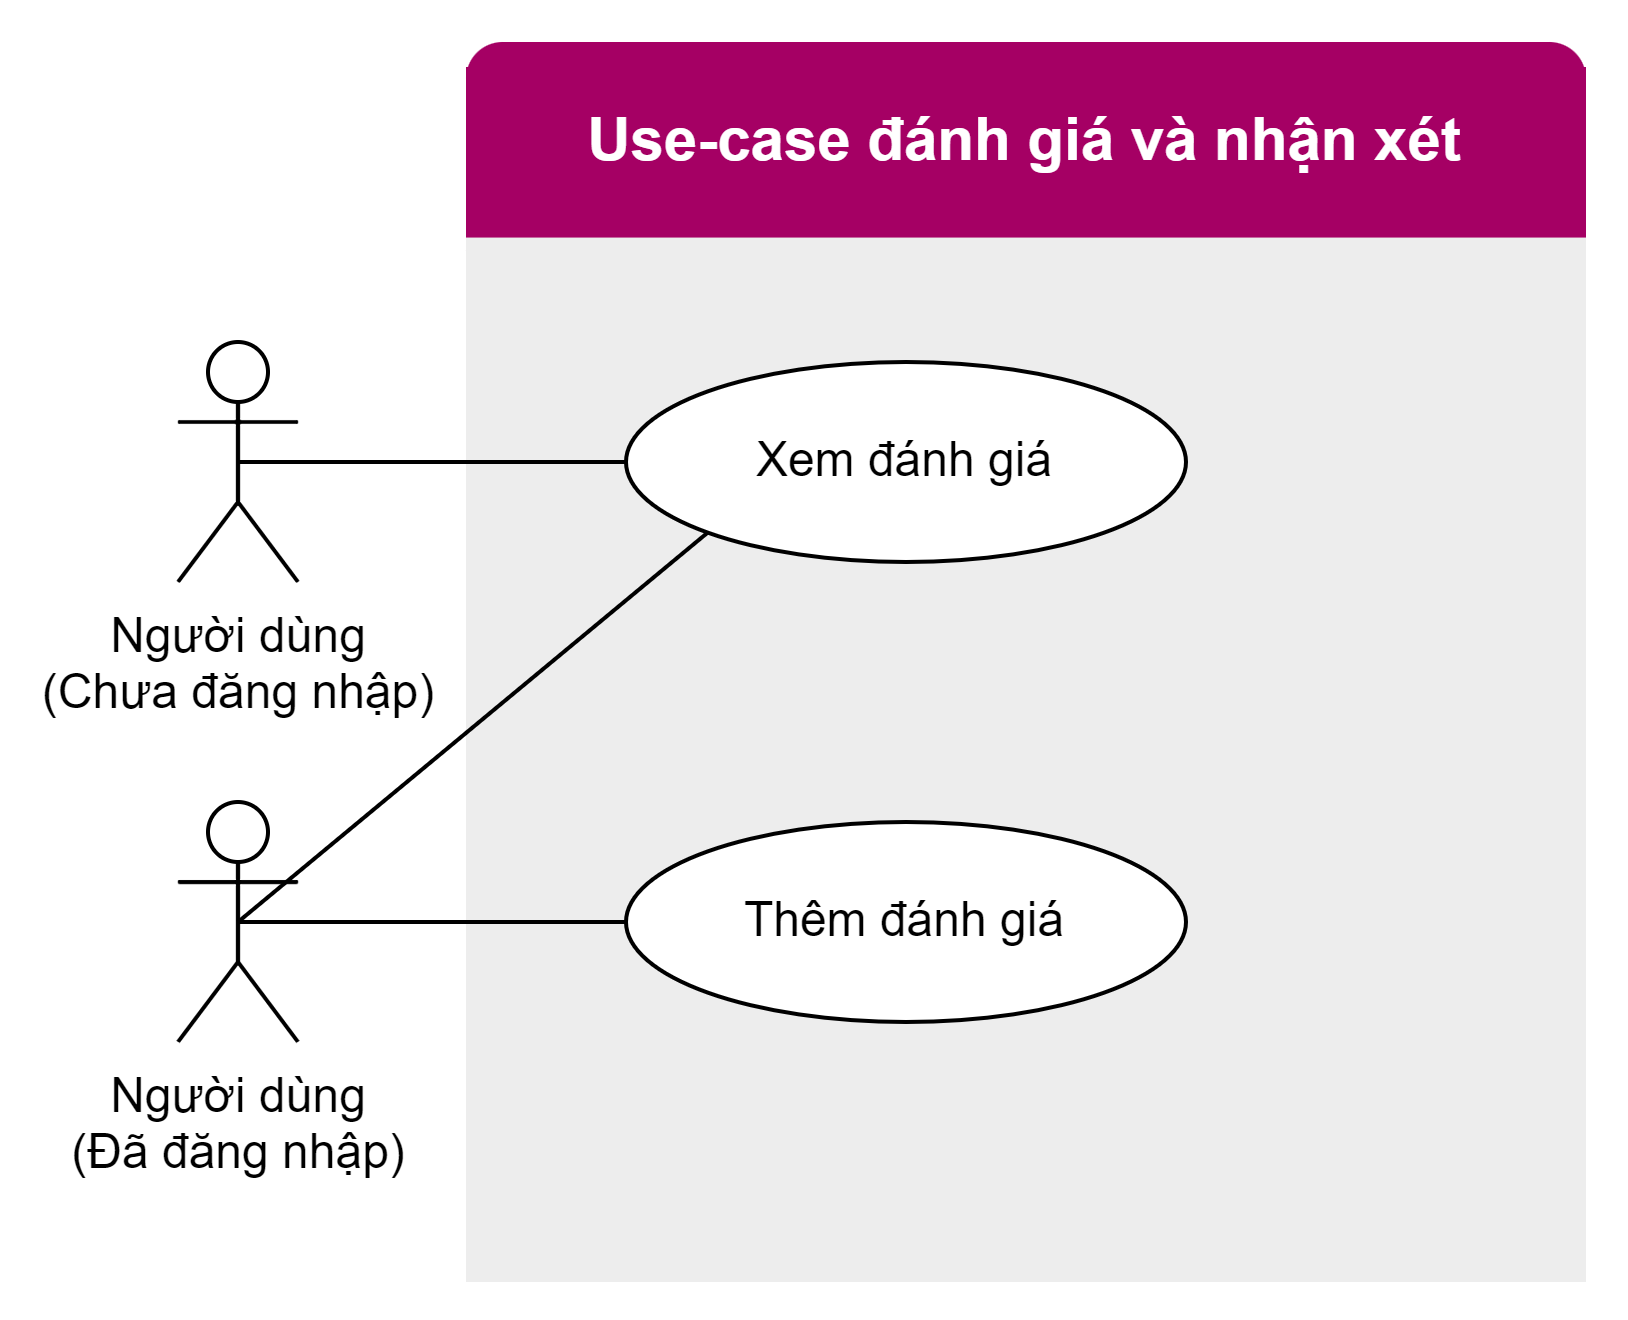
\includegraphics[width=10cm]{Images//usecase/use-case-nx.png}
            \newline
            \caption{Use-case diagram cho đánh giá và nhận xét}
            \label{fig:enter-label}
        \end{figure}
\end{enumerate}


\newpage
\subsubsection{Quản lý giảm giá (quản trị viên)}
\begin{enumerate}[a.]
    \item \textbf{ Use-case diagram}
    \begin{figure}[H]
            \centering
            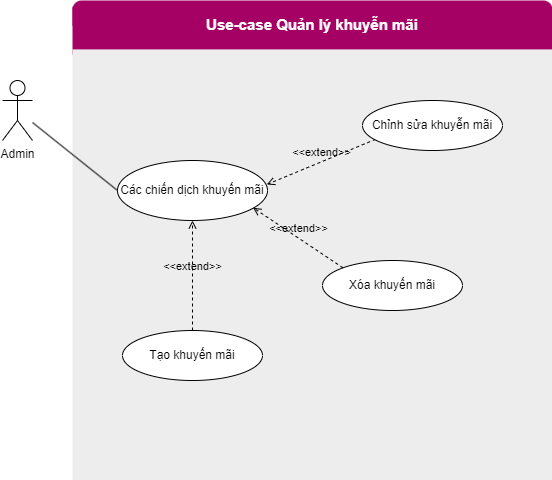
\includegraphics[width=10cm]{Images/usecase/Usecase_khuyenMai.drawio.png}
            \newline
            \caption{Use-case diagram cho quản lý khuyến mãi}
        \end{figure}
        \newpage
    \item \textbf{Mô tả use-case}
    \begin{enumerate}[]
    
        \begin{longtable}{|p{3.5cm}|p{11.5cm}|}
        \hline
        Name & Quản trị viên tạo mới một mã giảm giá \\ \hline
        Actor(s) &
          Quản trị viên \\ 
          \hline
        Description &
          Cho phép quản trị viên tạo mã giảm giá \\ 
          \hline
        Trigger &
          Quản trị viên muốn tạo mới một sự kiện giảm giá\\ 
          \hline
        Pre-condition(s) & \begin{tabular}[c]{@{}p{\linewidth}}
            Quản trị viên đang ở trang quản lý mã giảm giá và tích chọn tạo mới mã giảm giá. \\
        \end{tabular} \\ 
        \hline
        Post-condition(s) & Quản trị viên tạo mới thành công một mã giảm giá mới\\ 
        \hline
        Main Flow &
          \begin{tabular}[c]{@{}p{\linewidth}}
            1. Quản trị viên chọn tạo mới mã giảm giá cho toàn bộ khách hàng. \\
            2. Quản trị viên điền thống tin về chiến dịch khuyến mãi như tên, mô tả, khuyến mãi theo phần trăm (\%) hay giá tiền cố định, thời hạn; chọn tầm vực khách hàng hưởng khuyến mãi đó.\\
            3. Quản trị viên chọn lưu thay đổi.\\
            4. Hệ thống thoát ra khỏi màn hình tạo mới và đưa quản trị viên về lại trang quản lý khuyến mại và thêm mới chiến dịch khuyến mãi quản trị viên vừa tạo.
        \end{tabular} \\ \hline
        Alternative Flow &
          \begin{tabular}[c]{@{}p{\linewidth}} 
          \textbf{A1: Tại bước 2.}\\
           2.1. Quản trị viên bấm "Hủy" tạo mới.\\
           2.2. Hệ thống đưa quản trị viên về lại trang quản lý khuyến mãi. \\
        \end{tabular} \\ \hline
        Exception & None \\
        \hline
        \caption{Use-case tạo mới một khuyến mãi}
        \end{longtable}
        
        \newpage
        
    \begin{longtable}{|p{3.5cm}|p{11.5cm}|}
        \hline
        Name & Quản trị viên chỉnh sửa mã giảm giá \\ \hline
        Actor(s) &
          Quản trị viên \\ 
          \hline
        Description &
          Cho phép quản trị viên chỉnh sửa mã giảm giá \\ 
          \hline
        Trigger &
          Quản trị viên muốn chỉnh sửa sự kiện giảm giá\\ 
          \hline
        Pre-condition(s) & \begin{tabular}[c]{@{}p{\linewidth}}
            Quản trị viên đang ở trang quản lý chiến dịch giảm giá". \\
        \end{tabular} \\ 
        \hline
        Post-condition(s) & Quản trị viên chỉnh sửa thành công một mã giảm giá\\ 
        \hline
        Main Flow &
          \begin{tabular}[c]{@{}p{\linewidth}}
            1. Quản trị viên cần xác định chiến dịch nào cần thay đổi\\
            2. Quản trị viên nhấn vào biểu tượng chỉnh sửa của chiến dịch khuyến mãi mà admin muốn chỉnh sửa.\\
            3. Hệ thống chuyển quản trị viên vào màn hỉnh để chỉnh sửa thống tin của chiến dịch.\\
            4. Quản trị viên chọn lưu thay đổi.\\
            5. Hệ thống chuyển về màn hình quản lý khuyến mãi và cập nhật lại thống tin cho chiến dịch khuyến mãi.\\
        \end{tabular} \\ \hline
        Alternative Flow &
          \begin{tabular}[c]{@{}p{\linewidth}} 
          \textbf{A1: Tại bước 3.}\\
           3.1. Quản trị viên bấm "Hủy" chỉnh sửa.\\
           3.2. Hệ thống đưa quản trị viên về lại trang quản lý khuyến mãi. \\
        \end{tabular} \\ \hline
        Exception & None \\
        \hline
        \caption{Use-case chỉnh sửa khuyến mãi}
        \end{longtable}

        \newpage

    \begin{longtable}{|p{3.5cm}|p{11.5cm}|}
        \hline
        Name & Quản trị viên xóa chiến dịch giảm giá \\ \hline
        Actor(s) &
          Quản trị viên \\ 
          \hline
        Description &
          Cho phép quản trị viên xóa chiến dịch giảm giá \\ 
          \hline
        Trigger &
          Quản trị viên muốn xóa sự kiện giảm giá\\ 
          \hline
        Pre-condition(s) & \begin{tabular}[c]{@{}p{\linewidth}}
            Quản trị viên đang ở trang Quản lý mã giảm giá". \\
        \end{tabular} \\ 
        \hline
        Post-condition(s) & Quản trị viên xóa thành công một mã giảm giá\\ 
        \hline
        Main Flow &
          \begin{tabular}[c]{@{}p{\linewidth}}
            1. Quản trị viên cần xác định chiến dịch nào cần thay đổi\\
            2. Quản trị viên nhấn vào biểu tượng xóa của chiến dịch khuyến mãi mà quản trị viên muốn xóa.\\
            3. Hệ thống hiển thị một thống báo đến quản trị viên và yêu cầu nhấn vào nút "Xác nhận".\\
            4. Hệ thống chuyển màn hình sang trang Quản lý khuyến mãi và xóa chiến dịch khuyến mãi.\\
        \end{tabular} \\ \hline
        Alternative Flow &
          \begin{tabular}[c]{@{}p{\linewidth}} 
          \textbf{A1: Tại bước 3.}\\
           3.1. Quản trị viên bấm "Hủy" xóa.\\
           3.2. Hệ thống đưa quản trị viên về lại trang quản lý khuyến mãi. \\
        \end{tabular} \\ \hline
        Exception & None \\
        \hline
        \caption{Use-case xóa khuyến mãi}
        \end{longtable}
    \end{enumerate}
\end{enumerate}

\newpage

% \subsection{Quản lý thông báo (admin)}
% \subsubsection{Đẩy thông báo đến ứng dụng người dùng}
% \subsubsection{Chỉnh sửa thông báo}
% \subsubsection{Xóa thông báo}

\subsubsection{Quản lý khách hàng (quản trị viên)}
\begin{enumerate}[a.]
    \item \textbf{Use-case diagram}
    \begin{figure}[H]
            \centering
            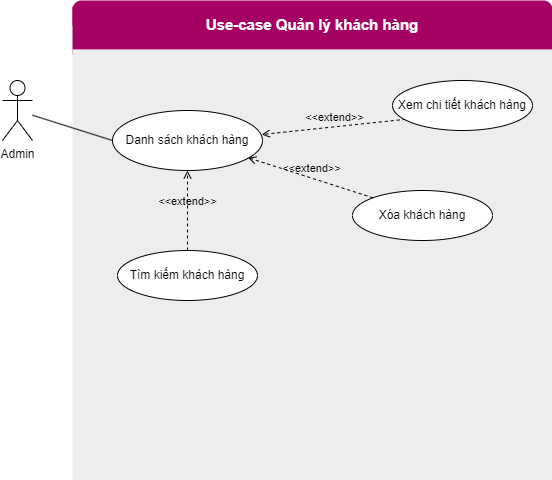
\includegraphics[width=15cm]{Images/usecase/Usecase_quanLyKhachHang.drawio.png}
            \newline
            \caption{Use-case diagram cho quản lý khách hàng}
            \label{figure_customerManagement}
        \end{figure}
    \newpage
    \item \textbf{Mô tả use-case}
    \begin{longtable}{|p{3.5cm}|p{11.5cm}|}
        \hline
        Name &
          Xem thông tin chi tiết của khách hàng \\ \hline
        Actor(s) &
          Quản trị viên \\ \hline
        Description &
          Cho phép quản trị viên xem thông tin chi tiết của tất cả các khách hàng trên hệ thống \\ \hline
        Trigger &
          Quản trị viên chọn nút "Quản lý khách hàng" tại trang giao diện chính của hệ thống\\ \hline
        Pre-condition(s) & \begin{tabular}[c]{@{}p{\linewidth}}
            - Quản trị viên đã đăng nhập vào hệ thống bằng tài khoản Manager\\
        \end{tabular} \\ 
          \hline
        Post-condition(s) &Quản trị viên xem được danh sách tất cả các khách hàng trong hệ thống.\\ \hline
        Main Flow &
          \begin{tabular}[c]{@{}p{\linewidth}}
            1 . Hệ thống hiển thị danh sách tất cả các khách hàng\\
        2 . Quản trị viên chọn cụ thể một khách hàng bằng cách nhấn vào nút icon xem chi tiết\\
        3 . Hệ thống hiển thị thông tin chi tiết của khách hàng\\
        \end{tabular} \\ \hline
        Alternative Flow &
          \begin{tabular}[c]{@{}p{\linewidth}} 
          \textbf{A1: Tại bước 1: }\\
         1.1. Quản trị viên nhấn tìm kiếm tên 1 khách hàng cụ thể\\
        1.2.Hệ thống trả về các khách hàng thỏa mãn tiêu chí tìm kiếm \\
        \end{tabular} \\ \hline
        Exception & None\\ 
        \hline
        \caption{Use-case xem thông tin chi tiết của khách hàng}
    \end{longtable}
    \newpage
    
    \begin{longtable}{|p{3.5cm}|p{11.5cm}|}
        \hline
        Name & Xóa khách hàng\\ \hline
        Actor(s) &
         Quản trị viên\\ \hline
        Description &
          Cho phép Quản trị viên xóa khách hàng khỏi hệ thống\\ \hline
        Trigger &
          Quản trị viên nhấn vào "Xóa khách hàng" \\ \hline
        Pre-condition(s) & \begin{tabular}[c]{@{}p{\linewidth}} 
        Quản trị viên đã đăng nhập vào tài khoản của mình\\
        Quản trị viên đang trong màn hình quản lý khách hàng\\
        Quản trị viên đã chọn được khách hàng muốn xóa\\   
        \end{tabular}\\
        \hline
          
        Post-condition(s) & Quản trị viên xóa thành công Khách hàng khỏi hệ thống\\ \hline
        Main Flow &
          \begin{tabular}[c]{@{}p{\linewidth}}
        1 . Hệ thống hiển thị 1 cảnh báo yêu cầu xác nhận xóa khách hàng.\\
        2 . Quản trị viên nhấn "Xác nhận xóa".\\
        3 . Hệ thống xác nhận xóa khách hàng thành công.\\
        4 . Quản trị viên nhấn "Xác nhận" để thoát khỏi giao diện xóa khách hàng và trở về giao diện quản lý khách hàng.
        \\
        \end{tabular} \\ \hline
        Alternative Flow & None\\ \hline 
        Exception & None \\ \hline
        \caption{Use-case xóa khách hàng}
    \end{longtable}
    \newpage

    \begin{longtable}{|p{3.5cm}|p{11.5cm}|}
        \hline
        Name &
          Tìm kiếm khách hàng\\ \hline
        Actor(s) &
          Quản trị viên \\ \hline
        Description &
          Cho phép Quản trị viên tìm kiếm khách hàng\\ \hline
        Trigger &
          \begin{tabular}[c]{@{}p{\linewidth}} 
        Quản trị viên nhấn vào ô tìm kiếm khách hàng\\
        
        \end{tabular} \\ \hline
        Pre-condition(s) & \begin{tabular}[c]{@{}p{\linewidth}} 
        Quản trị viên đã đăng nhập vào tài khoản của mình\\
        Quản trị viên đang trong màn hình quản lý khách hàng\\
        \end{tabular}\\
          \hline
        Post-condition(s) & Quản trị viên xem được thông tin khách hàng đã tìm kiếm\\ \hline
        Main Flow &
          \begin{tabular}[c]{@{}p{\linewidth}}
        1 . Quản trị viên nhập từ khóa tên của khách hàng cần tìm, rồi nhấn tìm kiếm\\
        2 . Hệ thống trả về danh sách tất cả khách hàng thỏa mãn yêu cầu của từ khóa \\
        \end{tabular} \\ \hline
        Alternative Flow & None
         \\ \hline
        Exception & \begin{tabular}[c]{@{}p{\linewidth}} 
        \textbf{E1: Tại bước 2:}\\
        - Hệ thống hiển thị lỗi "Không có khách hàng thỏa mãn yêu cầu"\\
        \end{tabular} \\ \hline
        \caption{Use-case tìm kiếm khách hàng}
    \end{longtable}
\end{enumerate}
\newpage


% \subsection{Hỗ trợ người dùng}
% \subsubsection{Hỗ trợ trực tuyến}
% \subsubsection{Những vấn đề hay gặp}

\subsubsection{Quản lý sản phẩm (admin)}
\begin{enumerate}[a.]
    \item \textbf{Use-case diagram}
        \begin{figure}[H]
            \centering
            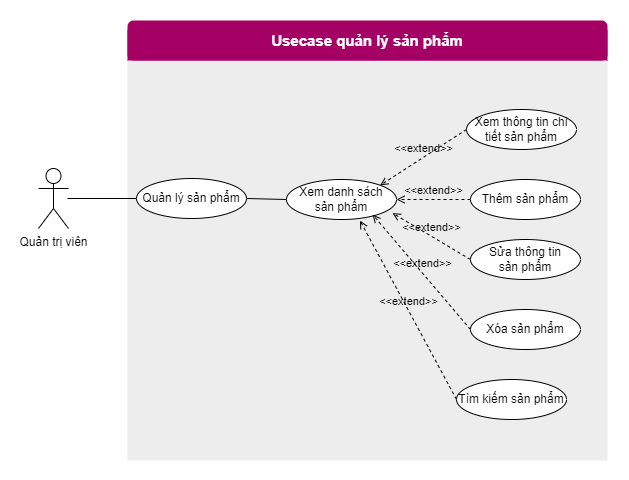
\includegraphics[width=15cm]{Images/usecase/ManageProduct.png}
            \caption{Use case diagram cho quản lý sản phẩm}
        \end{figure}
    \newpage
    \item \textbf{Mô tả usecase}
    \begin{longtable}{|p{3.5cm}|p{11.5cm}|}
        \hline
        Name &
          Xem thông tin chi tiết của sản phẩm \\ \hline
        Actor(s) &
          Quản trị viên \\ \hline
        Description &
          Cho phép quản trị viên xem thông tin chi tiết của tất cả các sản phẩm trên hệ thống \\ \hline
        Trigger &
          Quản trị viên chọn nút "Quản lý sản phẩm" tại trang giao diện chính của hệ thống\\ \hline
        Pre-condition(s) & \begin{tabular}[c]{@{}p{\linewidth}}
            - Quản trị viên đã đăng nhập vào hệ thống bằng tài khoản Manager\\
        \end{tabular} \\ 
          \hline
        Post-condition(s) &Quản trị viên xem được danh sách tất cả các sản phẩm trong hệ thống.\\ \hline
        
        Main Flow &
          \begin{tabular}[c]{@{}p{\linewidth}}
            1 . Hệ thống hiển thị danh sách tất cả các sản phẩm\\
        2 . Quản trị viên chọn cụ thể một sản phẩm bằng cách nhấn vào nút icon xem chi tiết\\
        3 . Hệ thống hiển thị thông tin chi tiết của sản phẩm\\
        \end{tabular} \\ \hline
        Alternative Flow &
          \begin{tabular}[c]{@{}p{\linewidth}} 
          \textbf{A1: Tại bước 1: }\\
         1.1. Quản trị viên nhấn tìm kiếm tên 1 sản phẩm cụ thể\\
        1.2.Hệ thống trả về các sản phẩm thỏa mãn tiêu chí tìm kiếm 
        \\
           
        \end{tabular} \\ \hline
          
        Exception & \begin{tabular}[c]{@{}p{\linewidth}} 
          None
        \end{tabular} \\ \hline
        \caption{Use-case xem thông tin chi tiết của sản phẩm}
    \end{longtable}
    \newpage
    
    \begin{longtable}{|p{3.5cm}|p{11.5cm}|}
        \hline
        Name &
          Quản lý sản phẩm - Thêm sản phẩm mới \\ \hline
        Actor(s) &
          Quản trị viên \\ \hline
        Description &
          Cho phép quản trị viên thêm một sản phẩm mới\\ \hline
        
        Trigger &
          Quản trị viên nhấn vào thêm sản phẩm\\ \hline
        
        Pre-condition(s) &
          \begin{tabular}[c]{@{}p{\linewidth}}
        Quản trị viên đã đăng nhập vào tài khoản của mình\\
        Quản trị viên đang trong màn hình quản lý sản phẩm\\
        
        \end{tabular} \\ \hline
          
        Post-condition(s) & Quản trị viên thêm sản phẩm thành công\\ \hline
        
        Main Flow &
          \begin{tabular}[c]{@{}p{\linewidth}}
        1 . Hệ thống chuyển sang giao diện nhập thông tin cho sản phẩm mới\\
        2 . Quản trị viên nhập lần lượt các thông tin mà hệ thống yêu cầu (tên sản phẩm, thể loại, giá bán, mô tả, ...)\\
        3 . Quản trị viên nhấn "Xác nhận" để thoát khỏi giao diện thêm sản phẩm\\
        4 . Hệ thống xác nhận thêm sản phẩm thành công\\
        \end{tabular} \\ \hline
        Alternative Flow &
          none \\ \hline
        Exception & \begin{tabular}[c]{@{}p{\linewidth}} 
        \textbf{E1: Tại bước 3:}\\
        - Hệ thống hiển thị lỗi "Tên/giá bán/... không hợp lệ"\\
        - Hệ thống hiển thị lỗi "Không được để trống thông tin"\\
        \end{tabular} \\ \hline
        \caption{Use-case thêm sản phẩm}
    \end{longtable}
    
    \begin{longtable}{|p{3.5cm}|p{11.5cm}|}
        \hline
        Name &
          Quản lý sản phẩm – Tìm kiếm sản phẩm\\ \hline
        Actor(s) &
          Quản trị viên \\ \hline
        Description &
          Cho phép quản trị viên tìm kiếm sản phẩm\\ \hline
        Trigger &
          \begin{tabular}[c]{@{}p{\linewidth}} 
        Quản trị viên nhấn vào ô tìm kiếm sản phẩm\\
        \end{tabular} \\ \hline
        Pre-condition(s) & \begin{tabular}[c]{@{}p{\linewidth}} 
        Quản trị viên đã đăng nhập vào tài khoản của mình\\
        Quản trị viên đang trong màn hình quản lý sản phẩm\\
        \end{tabular}\\
          \hline
        Post-condition(s) & Quản trị viên xem được thông tin sản phẩm đã tìm kiếm\\ \hline
        Main Flow &
          \begin{tabular}[c]{@{}p{\linewidth}}
        1 . Quản trị viên nhập từ khóa tên của sản phẩm cần tìm, rồi nhấn tìm kiếm\\
        2 . Hệ thống trả về danh sách tất cả sản phẩm thỏa mãn yêu cầu của từ khóa \\
        \\
        \end{tabular} \\ \hline
        Alternative Flow & None
         \\ \hline
        Exception & \begin{tabular}[c]{@{}p{\linewidth}} 
        \textbf{E1: Tại bước 2:}\\
        - Hệ thống hiển thị lỗi "Không có sản phẩm thỏa mãn yêu cầu"\\
        \end{tabular} \\ \hline
        \caption{Use-case tìm kiếm sản phẩm}
    \end{longtable}
    \newpage
    
    \begin{longtable}{|p{3.5cm}|p{11.5cm}|}
        \hline
        Name & Chỉnh sửa thông tin sản phẩm\\ \hline
        Actor(s) &
          Quản trị viên \\ \hline
        Description &
          Cho phép quản trị viên thay đổi thông tin sản phẩm trên hệ thống\\ \hline
        Trigger &
          Quản trị viên nhấn vào "Thay đổi thông tin sản phẩm" \\ \hline
        Pre-condition(s) & \begin{tabular}[c]{@{}p{\linewidth}} 
        Quản trị viên đã đăng nhập vào tài khoản của mình\\
        Quản trị viên đang trong màn hình quản lý sản phẩm\\
        Quản trị viên đã chọn được sản phẩm cần thay đổi thông tin\\
        \end{tabular}\\
        \hline
          
        Post-condition(s) & Quản trị viên đã thay đổi thông tin thành công cho sản phẩm\\ \hline
        
        Main Flow &
          \begin{tabular}[c]{@{}p{\linewidth}}
        1 . Hệ thống hiển thị 1 màn hình để chỉnh sửa các thông tin cần cho sản phẩm\\
        2 . Quản trị viên chỉnh sửa lần lượt các thông tin của sản phẩm
        3 . Quản trị viên nhấn "Cập nhật" để thoát khỏi giao diện chỉnh sửa thông tin sản phẩm\\
        4 . Hệ thống xác nhận chỉnh sửa thông tin sản phẩm thành công\\
        \end{tabular} \\ \hline
        Alternative Flow &
          None \\ \hline
        Exception & None \\ \hline
        \caption{Use-case chỉnh sửa thông tin sản phẩm}
    \end{longtable}
    
    \begin{longtable}{|p{3.5cm}|p{11.5cm}|}
        \hline
        Name & Xóa sản phẩm\\ \hline
        Actor(s) &
         Quản trị viên\\ \hline
        Description &
          Cho phép quản trị viên xóa sản phẩm khỏi hệ thống\\ \hline
        
        Trigger &
          Quản trị viên nhấn vào "Xóa sản phẩm" \\ \hline
        Pre-condition(s) & \begin{tabular}[c]{@{}p{\linewidth}} 
        Quản trị viên đã đăng nhập vào tài khoản của mình\\
        Quản trị viên đang trong màn hình quản lý sản phẩm\\
        B.M. đã chọn được sản phẩm muốn xóa\\   
        \end{tabular}\\
        \hline
          
        Post-condition(s) & Quản trị viên xóa thành công sản phẩm khỏi hệ thống\\ \hline
        
        Main Flow &
          \begin{tabular}[c]{@{}p{\linewidth}}
        1 . Hệ thống hiển thị 1 cảnh báo yêu cầu xác nhận xóa sản phẩm\\
        2 . Quản trị viên nhấn "Xác nhận xóa"\\
        3 . Hệ thống xác nhận xóa sản phẩm thành công\\
        4 . Quản trị viên nhấn "Xác nhận" để thoát khỏi giao diện xóa sản phẩm và trở về giao diện quản lý sản phẩm
        \\
        \end{tabular} \\ \hline
        Alternative Flow & None\\ \hline 
        Exception & None \\ \hline
        \caption{Use-case xóa sản phẩm}
    \end{longtable}
\end{enumerate}


\newpage
\subsubsection{Quản lý đơn hàng (admin)}
\begin{enumerate}[a. ]
    \item \textbf{Use-case diagram}
    \begin{figure}[h]
        \centering
        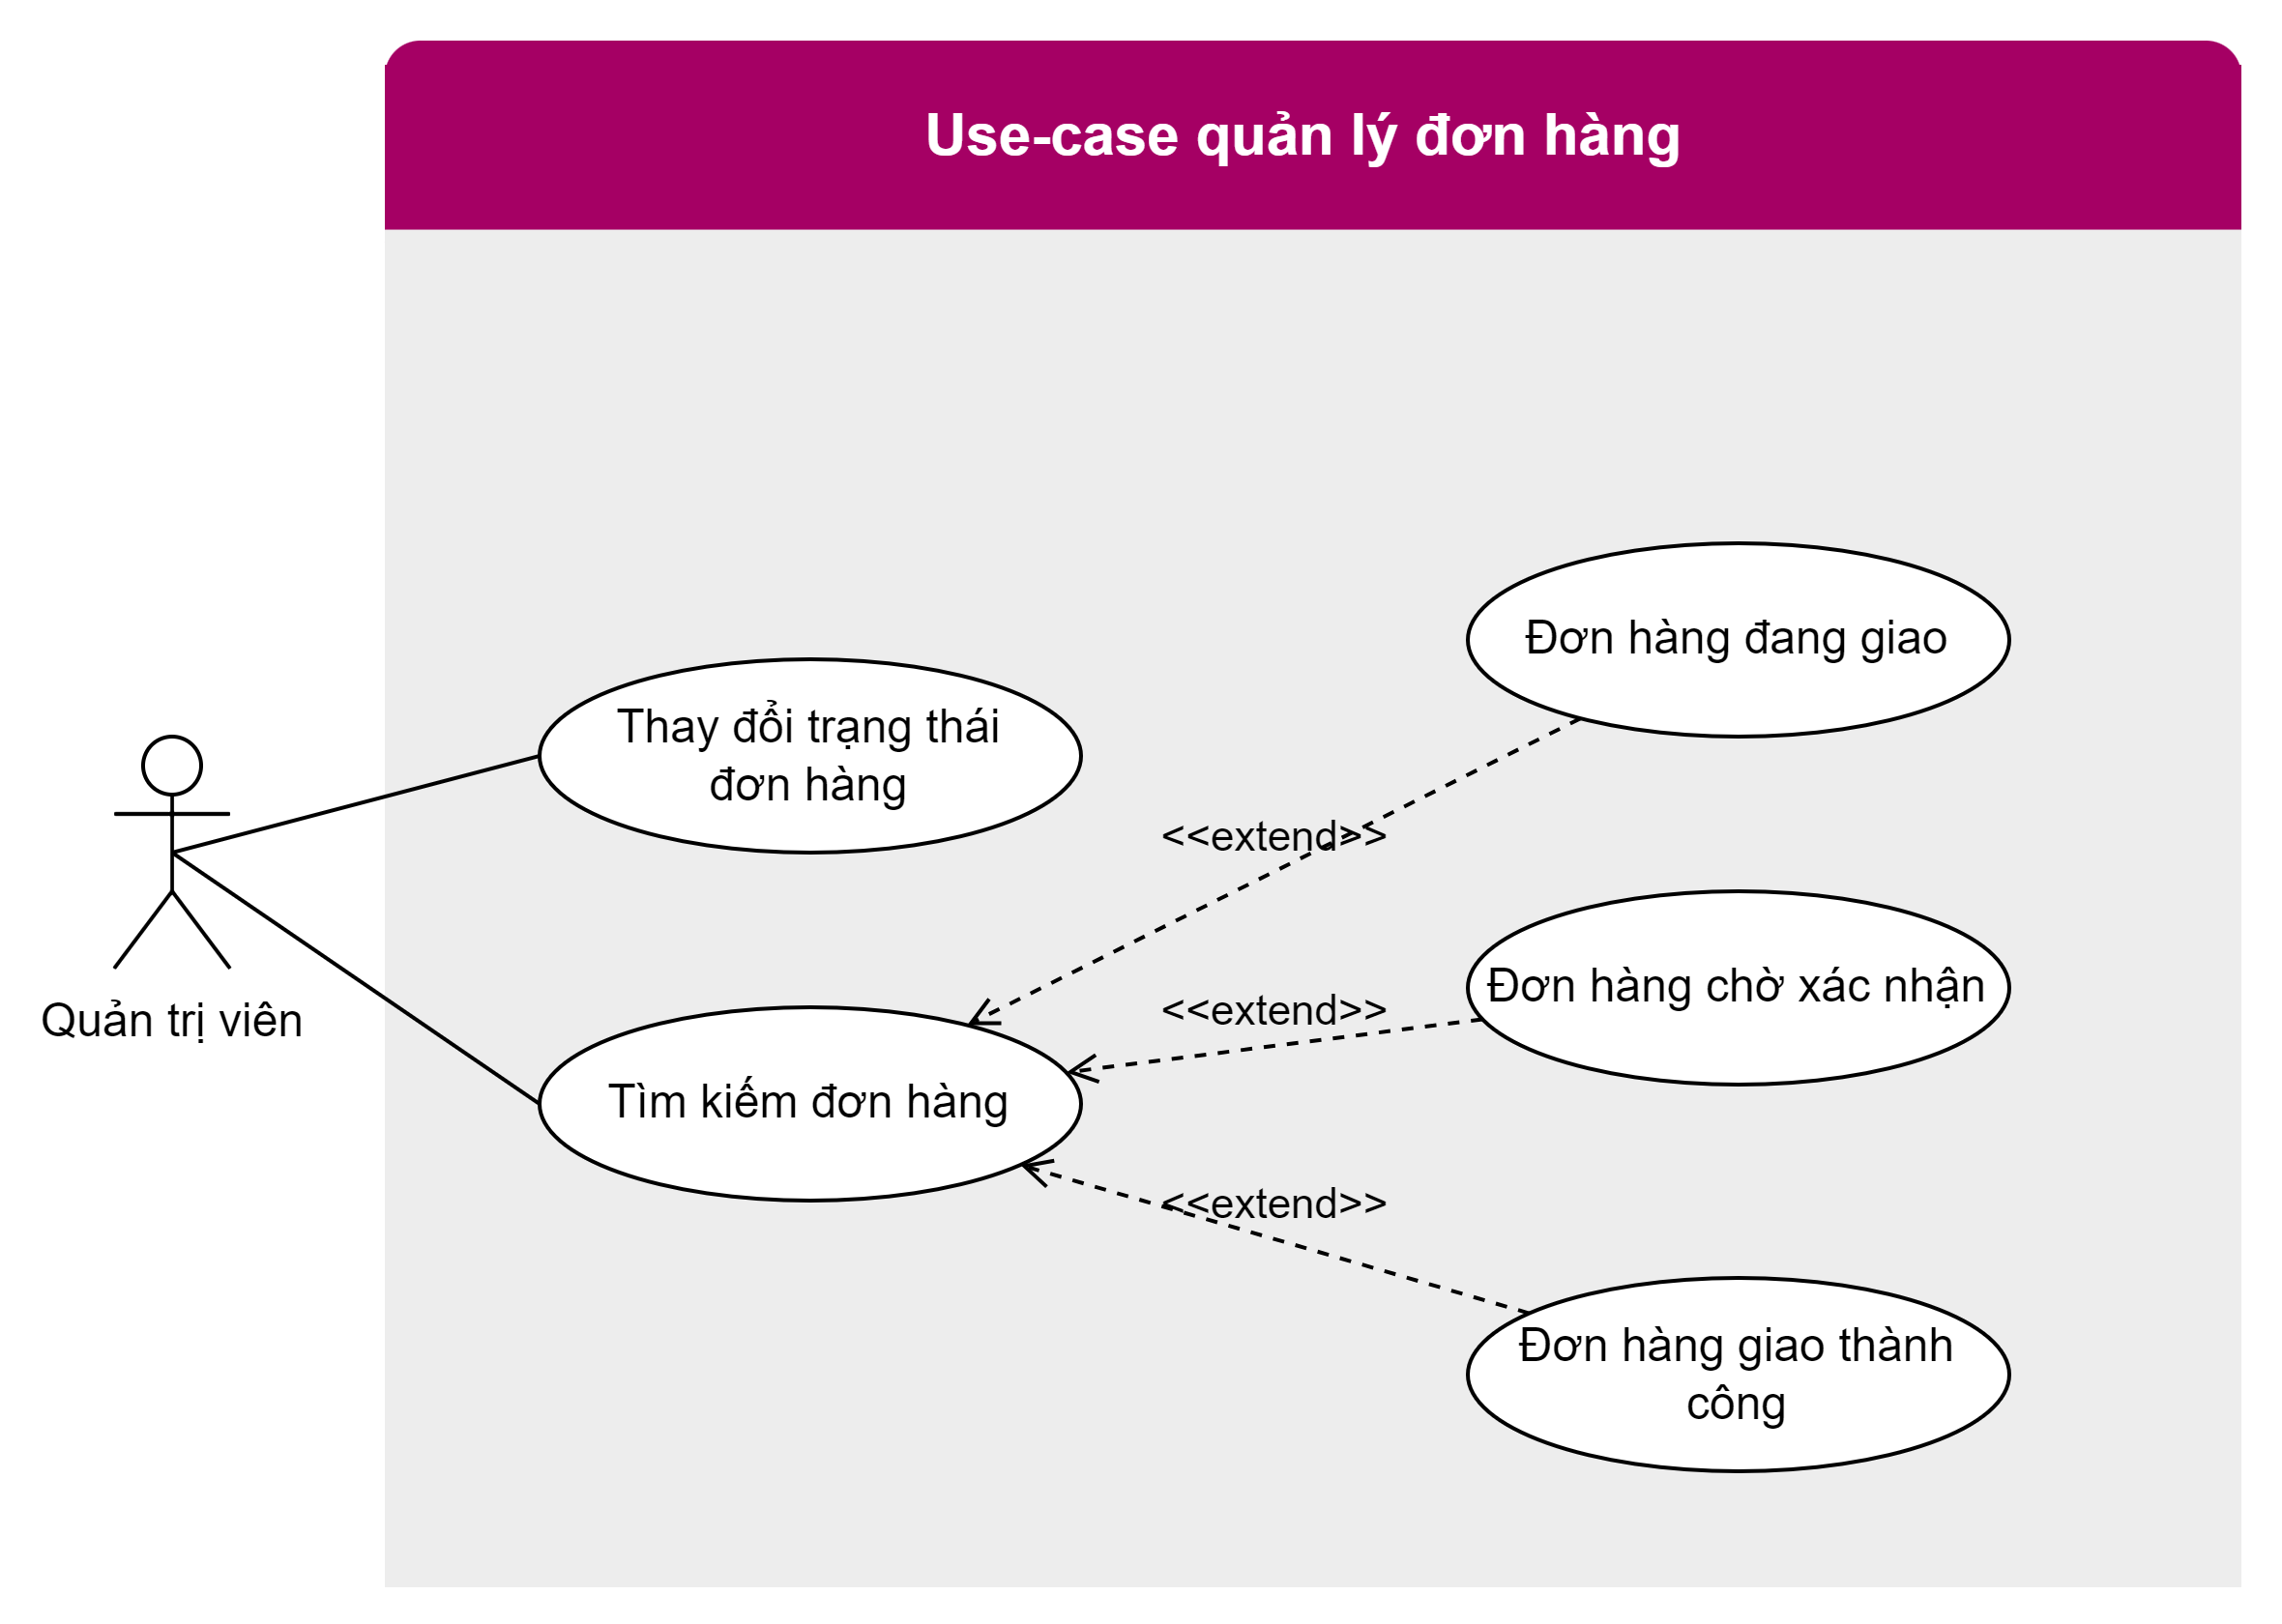
\includegraphics[width=10cm]{Images/usecase/use-case-manager-order.png}
        \newline
        \caption{Use-case diagram quản lý đơn hàng}
        \label{fig:enter-label}
    \end{figure}
    \item \textbf{Mô tả use-case}
    \begin{longtable}{|p{3.5cm}|p{11.5cm}|}
        \hline
        Name & Cập nhập trạng thái đơn hàng\\ \hline
        Actor(s) &
         Quản trị viên\\ \hline
        Description &
          Dùng để thay đổi trạng thái các đơn hàng như xác nhận để chuyển sang đang giao hàng và cuối cùng là giao hàng thành công\\ \hline
        
        Trigger & Cập nhập trạng thái đơn hàng \\ \hline
        Pre-condition(s) & \begin{tabular}[c]{@{}p{\linewidth}} 
        Quản trị viên đã đăng nhập vào tài khoản của mình \\
        Quản trị viên đang trong màn hình quản lý đơn hàng \\   
        \end{tabular}\\
        \hline
          
        Post-condition(s) & Cập nhập được trạng thái đơn hàng thành công\\ \hline
        Main Flow &
          \begin{tabular}[c]{@{}p{\linewidth}}
        1. Quản trị viên cần xác định đơn hàng cần thay đổi trạng thái \\
        2. Quản trị viên nhấn vào trạng thái đơn hàng và thay đổi \\
        3. Hệ thống hiện thông báo xác nhận thay đổi trạng thái đơn hàng\\
        4. Quản trị viên nhấn "Xác nhận" để thay đổi trạng thái đơn hàng.
        \\
        \end{tabular} \\ \hline
        Alternative Flow & None\\ \hline 
        Exception & None \\ \hline
        \caption{Use-case thay đổi trạng thái đơn hàng}
    \end{longtable}
\end{enumerate}
\subsection{Một số bài toán và giải pháp}
\subsubsection{Hệ thống gợi ý mua hàng}
\begin{enumerate}[a.]
\item \textbf{Khái niệm}\\
Hệ thống gợi ý mua hàng là một phần mềm hoặc công nghệ được sử dụng để cung cấp gợi ý và đề xuất sản phẩm cho người dùng dựa trên hành vi mua hàng trước đó, sở thích cá nhân, thông tin hồ sơ khách hàng, và các dữ liệu khác. Mục đích chính của hệ thống gợi ý mua hàng là cung cấp trải nghiệm mua hàng cá nhân hóa, tăng khả năng tương tác và mua hàng của khách hàng, và tăng doanh số bán hàng cho các doanh nghiệp.
\item \textbf{Các phương pháp hiện có}\\
Các hệ thống gợi ý mua hàng thường sử dụng các phương pháp và thuật toán khác nhau để đưa ra gợi ý sản phẩm. Dưới đây là một số phương pháp phổ biến:
\begin{itemize}
    \item \textbf{Gợi ý dựa trên sở thích cá nhân:} Hệ thống phân tích và đánh giá sở thích cá nhân của người dùng dựa trên lịch sử mua hàng, đánh giá sản phẩm, hoặc thông tin cá nhân khác để đề xuất các sản phẩm phù hợp.
    \item \textbf{Gợi ý dựa trên hành vi mua hàng tương tự:} Hệ thống phân tích hành vi mua hàng của người dùng và tìm kiếm những người dùng có hành vi mua hàng tương tự để đề xuất các sản phẩm mà họ có thể quan tâm.
    \item \textbf{Gợi ý dựa trên phân tích nội dung:}  Hệ thống phân tích nội dung sản phẩm, ví dụ: mô tả sản phẩm, danh mục, hoặc nguồn gốc, để đề xuất các sản phẩm tương tự hoặc liên quan.
    \item \textbf{Gợi ý dựa trên gom cụm (clustering): }Hệ thống phân tích và nhóm các sản phẩm vào các nhóm tương tự nhau và đề xuất các sản phẩm từ cùng một nhóm hoặc nhóm liên quan.
    \item \textbf{Gợi ý dựa trên kết hợp nhiều phương pháp:} Hệ thống kết hợp nhiều phương pháp và thuật toán để đưa ra gợi ý mua hàng chính xác và đa dạng.
\end{itemize}
\item \textbf{Hiện thực}\\
Trong nghiên cứu này, chúng tôi đã áp dụng công nghệ đồ thị của Neo4j vào hệ thống gợi ý mua hàng thông minh. Neo4j, một hệ quản trị cơ sở dữ liệu đồ thị phổ biến, cho phép chúng tôi lưu trữ và truy vấn dữ liệu có tính chất mối quan hệ phức tạp, như mối quan hệ giữa khách hàng, sản phẩm và các yếu tố khác.

Trước tiên, chúng tôi đã mô hình hóa thông tin về khách hàng bằng cách tạo các node đại diện cho khách hàng trong Neo4j. Mỗi node chứa các thuộc tính như sở thích cá nhân, lịch sử mua hàng, đánh giá sản phẩm và các thông tin cá nhân khác. Điều này giúp chúng tôi hiểu rõ hơn về sở thích và nhu cầu của từng khách hàng.

Tiếp theo, chúng tôi đã mô hình hóa các sản phẩm bằng cách tạo các node đại diện cho chúng trong Neo4j.
\begin{itemize}
    \item Product(id)
    \item User(id, phone\_number)
    \item Category(id)
\end{itemize}
Chúng tôi đã tạo các mối quan hệ giữa các sản phẩm dựa trên sự tương tự hoặc sự liên quan, cho phép chúng tôi tìm ra các mẫu và xu hướng trong dữ liệu sản phẩm. 
\begin{itemize}
    \item ADD\_TO\_WISH\_LISH(add\_at): Đây là mối quan hệ giữa User và Product. Mô tả cho việc User thêm sản phẩm vào mục yêu thích.

    \item BOUGHT(bought\_at): Đây là mối quan hệ giữa User và Product. Thể hiện việc khách hàng đã mua sản phẩm này.

    \item VIEWED(viewed\_at): Đây là mối quan hệ giữa User và Product. Thể hiện việc khách hàng đã ấn vào xem chi tiết sản phẩm.

    \item ADD\_TO\_CART(add\_at, variant\_id, quantity): Đây là mối quan hệ giữa User và Product. Thể hiện khách hàng đã thêm một sản phẩm vào giỏ hàng. Đây sẽ là nơi lưu giỏ hàng của khách hàng. Nhằm đảm bảo việc khách hàng dùng nhiều điện thoại thì giỏ hàng vẫn sẽ đồng bộ trên nhiều thiết bị.

    \item IS\_IN: Đây là mối quan hệ giữa Product và Category. Thể hiện việc product này thuộc về category nào
\end{itemize}
Chúng tôi đã sử dụng Neo4j để tạo các mối quan hệ giữa khách hàng và sản phẩm. Ví dụ, chúng tôi đã tạo mối quan hệ "BOUGHT" giữa khách hàng và các sản phẩm đã mua, cũng như mối quan hệ "VIEWED" giữa khách hàng và các sản phẩm đã xem. Điều này cho phép chúng tôi theo dõi hành vi mua hàng và gợi ý các sản phẩm phù hợp dựa trên sở thích và hành vi của khách hàng.

Để đề xuất các sản phẩm gợi ý, chúng tôi đã sử dụng truy vấn Neo4j để tìm kiếm các sản phẩm phù hợp. Ngoài ra chúng tôi sẽ sắp xếp dựa theo ngày mua của những sản phẩm để lấy ra sản phẩm cần gợi ý để tránh trường hợp sản phẩm khách hàng đã mua khá lâu còn gợi ý. Sau đây là một số phương pháp gợi ý mà chúng tôi sẽ áp dụng vào dự án.

\textbf{Gợi ý sản phẩm dựa trên những hành vi mua hàng tương tự nhau}

Phương pháp này phân tích bằng việc người dùng A và B có điểm chung gì trong việc mua hàng, xem sản phẩm và thêm vào yêu thích. Đầu tiên là A và B cùng mua 1 sản phẩm là Y và B cũng có mua thêm sản phẩm Z, thì lúc này hệ thống sẽ tính toán và trả về Z là sản phẩm cần gợi ý đến A.

Đầu tiên chúng tôi thực hiện lấy ra những sản phẩm dựa trên câu lệnh trên neo4j và sẽ nhận được kết quả là 1 danh sách các sản phẩm được gợi ý. Sau đó thực hiện lấy những sản phẩm đó từ trong database trả về cho người dùng.

\textbf{Gợi ý sản phẩm dựa trên những sản phẩm đã xem}

Đầu tiên chúng tôi sẽ lấy những sản phẩm mà khách hàng đã xem từ trong database được sắp xếp theo thời gian xem.

Sau đó chúng tôi sẽ lấy lần lượt những category trong sản phẩm. Bởi vì một sản phẩm có thể có nhiều category nên chúng tôi sẽ kiểm tra dựa trên những sản phẩm phải bao gồm luôn cả category trong sản phẩm đã mua đó. Nó sẽ trả về một danh sách của những category của sản phẩmVí dụ: sản phẩm A có category X1 và X2, sản phẩm B có Category là X3, X4 lúc này chúng ta sẽ trả về những danh sách category để thực hiện tìm kiếm: [[X1, X2], [X3, X4]]. Có nghĩa là ta sẽ lấy ra những sản phẩm có cùng category (điều kiện hợp) trong từng danh sách trên (điều kiện giao).

Thực hiện query những sản phẩm có category rồi trả về giao diện bán hàng.

\end{enumerate}
Bằng cách sử dụng Neo4j, chúng tôi đã tận dụng được tính năng mạnh mẽ của công nghệ đồ thị để lưu trữ và truy vấn dữ liệu một cách hiệu quả. Chúng tôi đã sử dụng ngôn ngữ truy vấn Cypher của Neo4j để tạo và truy vấn các node, mối quan hệ và thuộc tính trong hệ thống gợi ý mua hàng. Điều này đã giúp chúng tôi xây dựng một hệ thống gợi ý mua hàng thông minh hiệu quả và tốt
% \subsubsection{Hệ thống phân loại sản phẩm theo xu hướng thời trang}
\subsubsection{Hệ thống thanh toán}
\textbf{Cổng thanh toán PayOS}

Trong dự án này chúng tôi sử dụng thanh toán bằng hình thức chuyển khoản ngân hàng thông qua cổng thanh toán PayOS. Đây là cổng thanh toán thông qua VietQrPro. Ưu điểm của việc sử dụng cổng thanh toán này là không cần phải là doanh nghiệp thì mới có thể tích hợp cổng thanh toán mà chúng ta có thể tạo cổng thanh toán khi mà ta có thẻ ngân hàng và căn cước công dân.

Ngoài ra cổng thanh toán này còn hỡ trợ kiểm tra giao dịch real time (bắn Webhook về cho hệ thống chúng tôi). Sau đó chúng tôi sẽ dùng socket io để bắn giao dịch thành công đến ứng dụng khách hàng. Điều này sẽ làm cho việc mua hàng và thanh toán của người dùng mượt mà hơn, khi người dùng thanh toán thành công trên thiết bị của mình thì thông tin trạng thái thanh toán đơn hàng sẽ được tự động cập nhập.

\noindent Luồng thực thi của cổng PayOS

Sau khi người người dùng bâm thanh toán, sẽ chuyển người dùng đến trang thanh toán, đồng thời tạo một kết nối đến hệ thống để hệ thống có thể bắn message về ứng dụng khi đơn hàng thanh toán thành công.

Ở trên ứng dụng, khi người dùng đã thanh toán đơn hàng thành công thì lúc này hệ thống sẽ được PayOS gọi đế một API đã được định nghĩa sẵn ở hệ thống để nhận thông tin thanh toán, sau đó hệ thống sẽ lưu vào cơ sở dữ liệu đồng thời bắn message thanh toán thành công đến ứng dụng.
\begin{figure}[H]
    \centering
    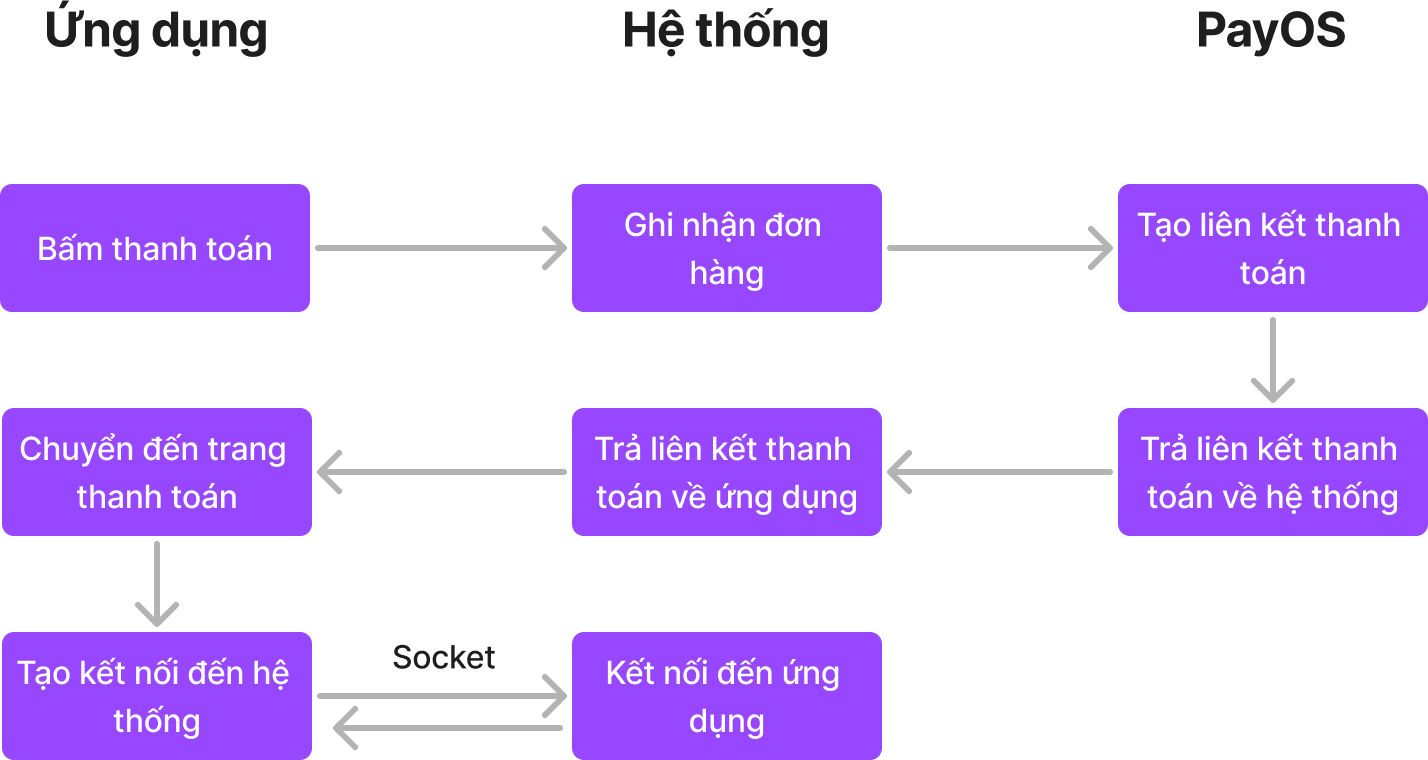
\includegraphics[width=15cm]{Images/payos-1.png}
    \newline
    \caption{Tạo connection đến ứng dụng}
    \label{fig:enter-label}
\end{figure}



\begin{figure}[H]
    \centering
    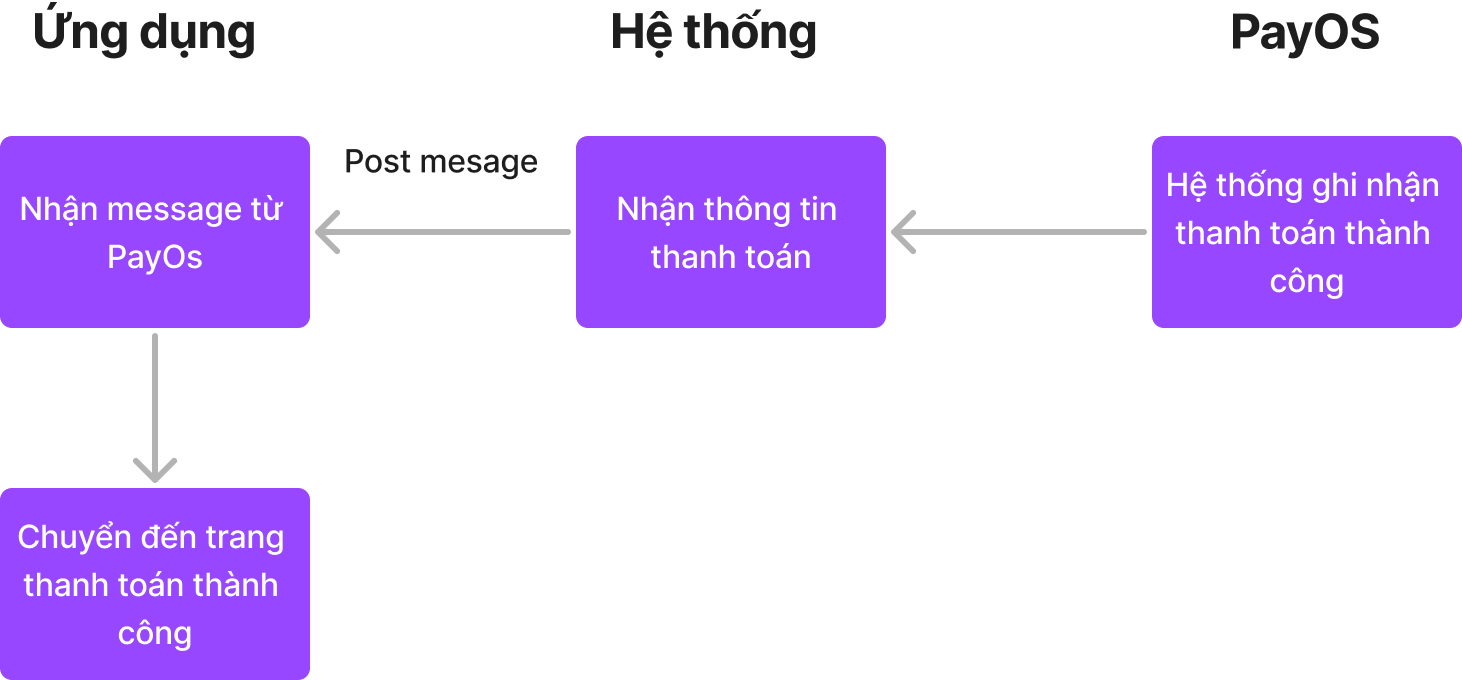
\includegraphics[width=15cm]{Images/payos-2.png}
    \newline
    \caption{Bắn message đến cho ứng dụng}
    \label{fig:enter-label}
\end{figure}

\subsubsection{Lọc và vô hiệu hóa các bình luận, đánh giá sản phẩm vi phạm tiêu chuẩn}
\begin{enumerate}[a.]
\item \textbf{Giới thiệu}\\
Mục tiêu là kiểm tra và loại bỏ các đánh giá/bình luận có chứa nội dung phản cảm dựa trên một số tiêu chí như chứa liên kết URL, sử dụng từ ngữ xấu, mức độ độc hại theo các tiêu chí như tấn công danh tính, xúc phạm, ngôn ngữ thô tục, độc hại nghiêm trọng, nội dung tình dục rõ ràng, đe dọa và độc hại.

\item \textbf{Mô tả giải thuật}\\
\textbf{Kiểm tra đường dẫn URL} \\
Sử dụng biểu thức chính quy (regular expression) để kiểm tra các đường dẫn URL, sau đó kiểm tra sự tồn tại của URL đó có chứa trong nội dung hay không. \\
\textbf{Kiểm tra từ ngữ xấu}\\
Sử dụng hàm badWords của thư viện vn-badwords để kiểm tra sự hiện diện của các từ ngữ cấm trong nội dung đánh giá sản phẩm. Hàm badWords sẽ kiểm tra nội dung có chứa các từ ngữ cấm hay không. Nếu có, hàm trả về true, ngụ ý rằng đánh giá sản phẩm sẽ bị vô hiệu hóa.\\
\textbf{Phân loại mức độ độc hại}\\
Sử dụng mô hình học sâu từ thư viện toxicity của Tensorflow: Hàm sử dụng mô hình này để phân loại nội dung dựa trên các tiêu chí độc hại. \\
Giá trị ngưỡng 0.9 được sử dụng để xác định độ nhạy của mô hình. Ngưỡng này có nghĩa là mô hình chỉ coi nội dung là phản cảm nếu độ tin cậy của kết quả phân loại cao hơn 90\%. Các nhãn (labels) mà mô hình này kiểm tra bao gồm: identity attack (tấn công danh tính), insult (xúc phạm), obscene (ngôn ngữ thô tục), severe toxicity (độc hại nghiêm trọng), sexual explicit (nội dung tình dục rõ ràng), threat (đe dọa) và toxicity (độc hại). Mô hình được tải với ngưỡng và các nhãn này để phân loại nội dung đánh giá sản phẩm.\\
Mô hình sẽ phân loại nội dung và trả về kết quả dưới dạng các nhãn với giá trị match (đúng hoặc sai) cho từng tiêu chí. Nếu bất kỳ nhãn nào xác định rằng nội dung là phản cảm (kết quả match là true), đánh giá sản phẩm sẽ bị đánh dấu là vi phạm tiêu chuẩn.
\end{enumerate}

\subsubsection{Tính năng tìm kiếm sản phẩm bằng hình ảnh}

\begin{enumerate}[a.]
\item \textbf{Khái niệm}\\
Tính năng tìm kiếm sản phẩm bằng hình ảnh là một công cụ mạnh mẽ và tiện ích trong các ứng dụng bán hàng trực tuyến, đặc biệt là ứng dụng bán quần áo. Tính năng này cho phép người dùng tải lên một bức ảnh của một sản phẩm (ví dụ như một chiếc áo sơ mi, một đôi giày, v.v.) và hệ thống sẽ tự động nhận diện và tìm kiếm các sản phẩm tương tự hoặc giống với sản phẩm trong bức ảnh đó trong cơ sở dữ liệu của cửa hàng.\\
\item \textbf{Mô tả giải thuật}


Tính năng này được xây dựng dựa trên phương pháp Content-based Image Retrieval (CBIR). Ảnh của các sản phẩm sau khi được lưu và ảnh của sản phẩm mà người dùng muốn tìm sẽ tiến hành trích xuất đặc trưng (feature extraction). \\
Trích xuất đặc trưng của ảnh (image feature extraction) là quá trình chuyển đổi hình ảnh từ dạng thô (các điểm ảnh) thành một vector đặc trưng (feature vector) mà máy tính có thể xử lý và hiểu. Chúng tôi sử dụng VGG16 model được tích hợp sẵn vào keras và được huấn luyện trước trên bộ dữ liệu ImageNet để thực hiện quá trình này.\\
Cấu hình mô hình: Tạo ra một hình con từ VGG16. Mô hình con này sẽ lấy đầu vào là hình ảnh và đầu ra là lớp fc1 của VGG16.\\
\textbf{Các bước trích xuất đặc trưng(feature extraction):}
\begin{enumerate}[1.]
    \item Mở hình ảnh từ buffer và chuyển đổi nó thành đối tượng PIL Image.
    \item Ảnh được chuyển sang dạng tensor trước khi đưa vào mô hình để trích xuất
    \item Đưa tensor vào mô hình tiến hành trích xuất đặc trưng. Nhận lại là một vector đặc trưng.
    \item Chuẩn hóa vector đặc trưng thành độ dài là 1. Điều này giúp thuận lợi trong quá trình so sánh vector sau này
\end{enumerate}
\textbf{Giải thuật Search by image:}
\begin{figure}[H]
    \centering
    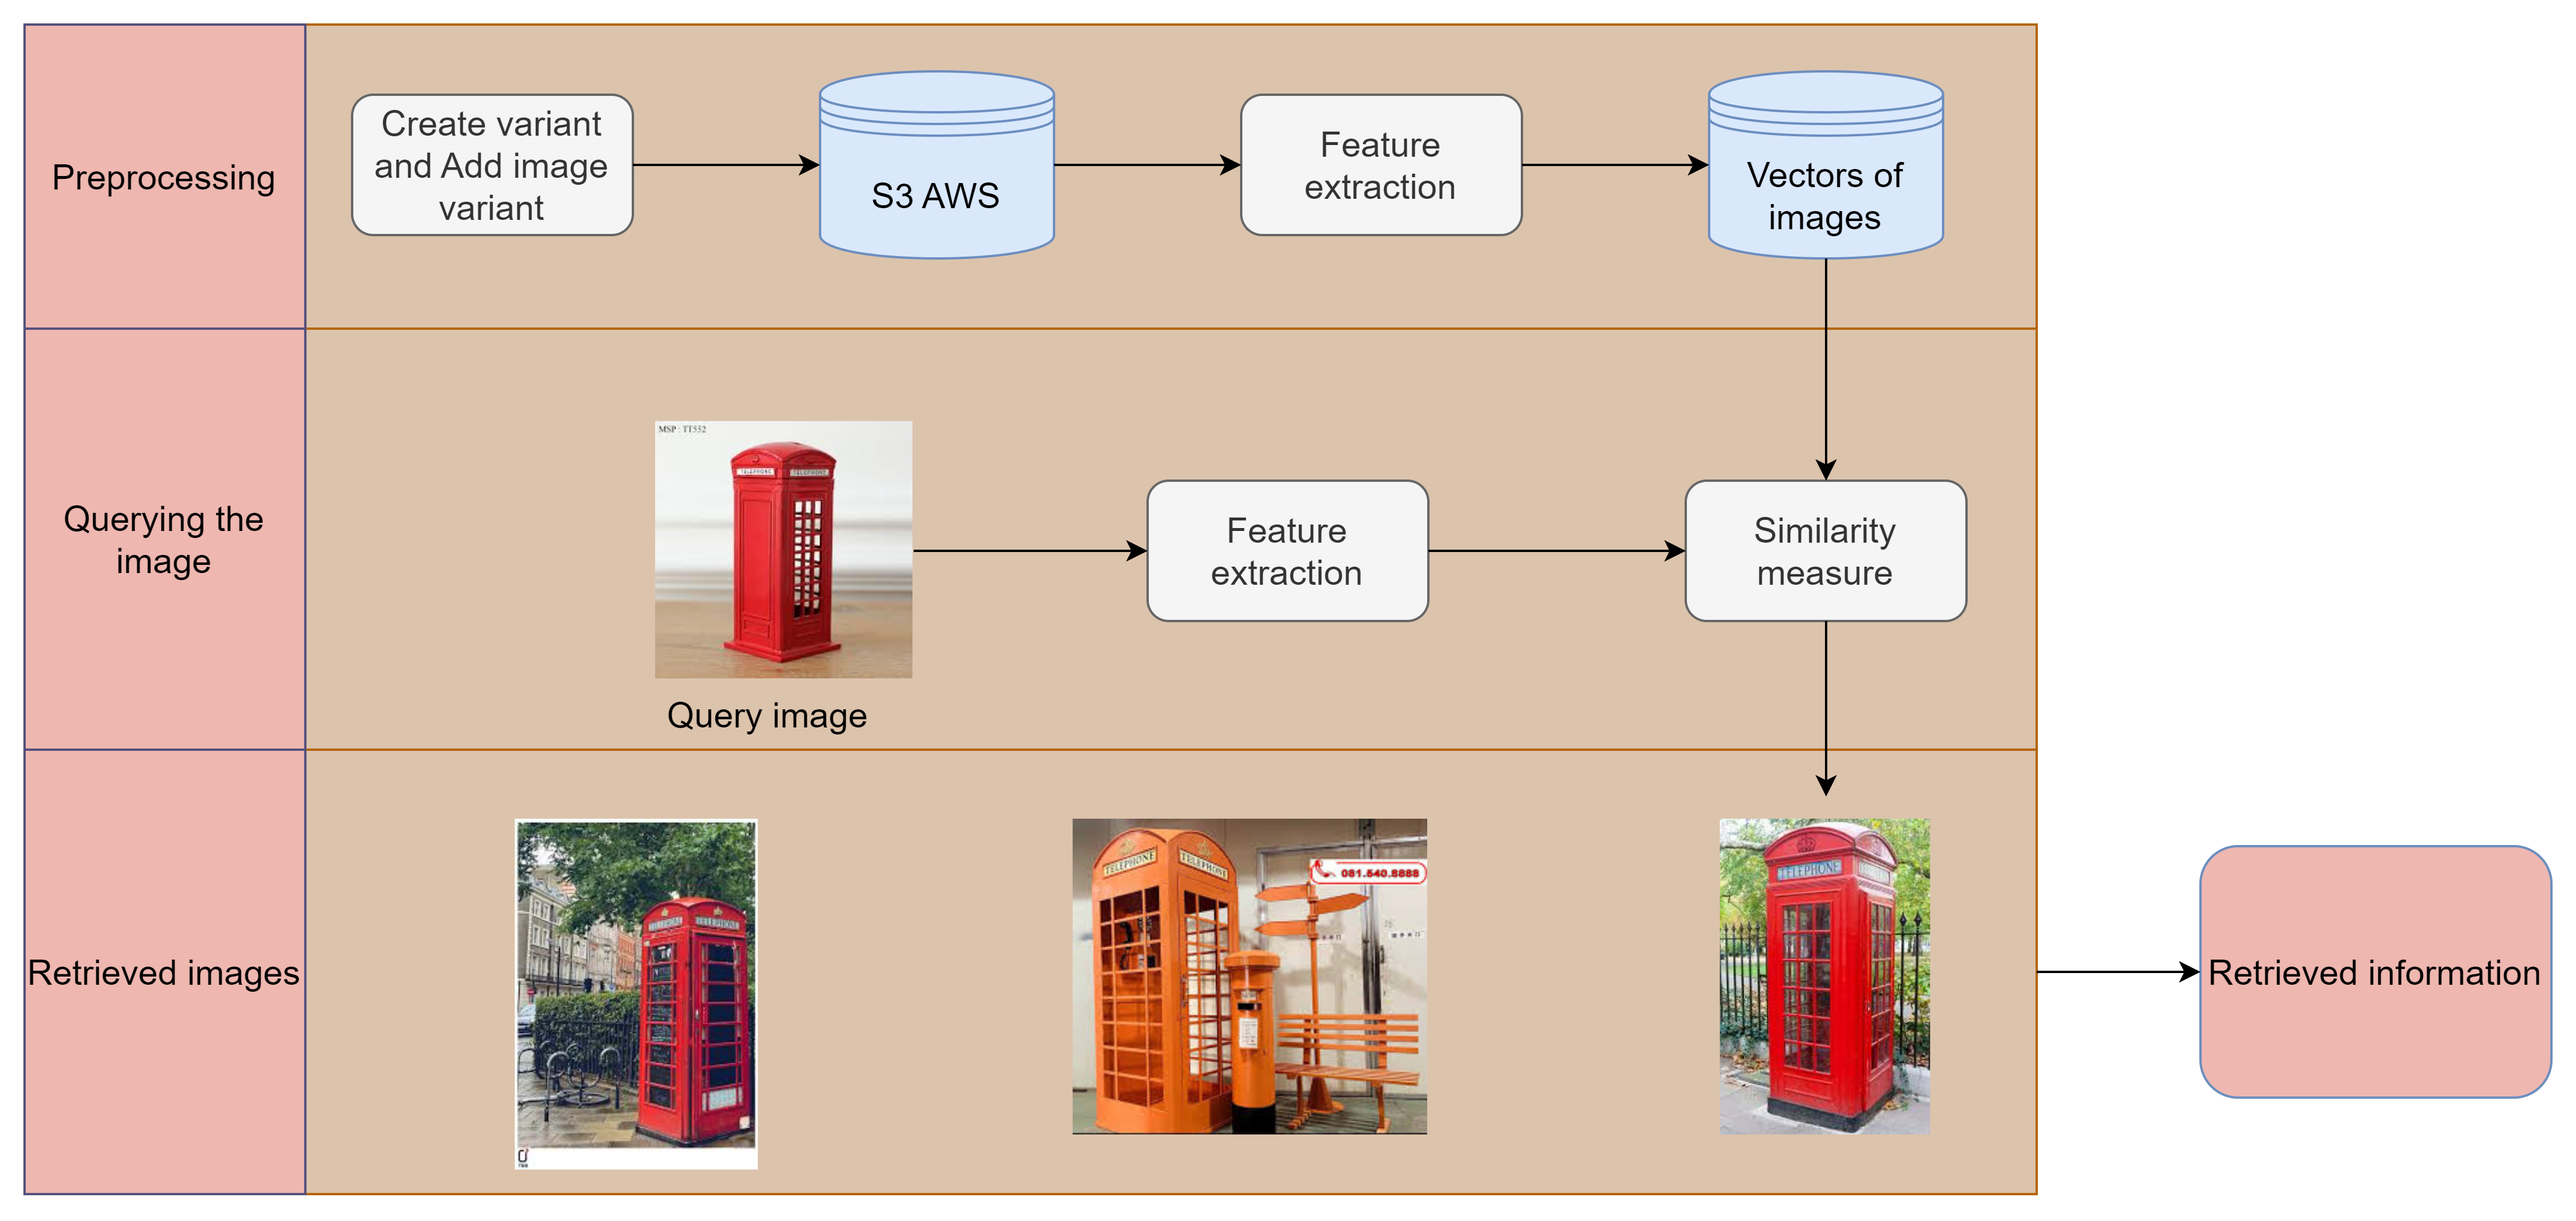
\includegraphics[width=15cm]{Images/search_by_image.png}
    \newline
    \caption{Giải thuật Search by image}
    % \label{fig:enter-label}
\end{figure}
\begin{enumerate}[1.]
    \item Preprocessing: Sau khi tạo variant và thêm ảnh lên S3 AWS. Các ảnh đó được tải lên và tiến hành trích xuất đặc trưng. Cuối cùng lưu vào kho chứa vector của ảnh.
    \item Querying the Image:  Người dùng cung cấp một hình ảnh truy vấn. Ảnh đó được tải lên và tiến hành trích xuất thành vector. Vector đó được đo khoảng cách với từng vector trong kho chứa vector bằng phương pháp tính khoảng cách Euclid. Từ đó, ta được danh sách các khoảng cách.

    \newpage
    \item Retrieved Images: Lấy ra các khoảng cách có giá trị thấp nhất, từ đó lấy được các ảnh và sản phẩm tương đồng với ảnh người dùng cung cấp
\end{enumerate}
\item \textbf{Hiện thực}\\
\noindent FastAPI là một framework hiện đại, nhanh chóng, và dễ sử dụng để phát triển các API với Python. Nó được xây dựng trên các công nghệ tiên tiến như ASGI (Asynchronous Server Gateway Interface) và sử dụng các thư viện mạnh mẽ như Starlette và Pydantic để cung cấp một trải nghiệm phát triển hiệu quả và mạnh mẽ.\\
Các ưu điểm của FastAPI:
\begin{itemize}
    \item Hiệu suất cao
    \item Dễ sử dụng
    \item Tài liệu tự động
    \item Xác thực và kiểm tra dữ liệu mạnh mẽ
    \item Hỗ trợ các tính năng hiện đại của Python
    \item Tích hợp dễ dàng với các thư viện khác
\end{itemize}
Vì các lý do trên, chúng tôi chọn xây dựng các API hỗ trợ cho tính năng Search by image bằng FastAPI.


\end{enumerate}









\newpage

\section{Thiết kế hệ thống}
\subsection{Kiến trúc tổng thể}

\begin{figure}[H]
    \centering
    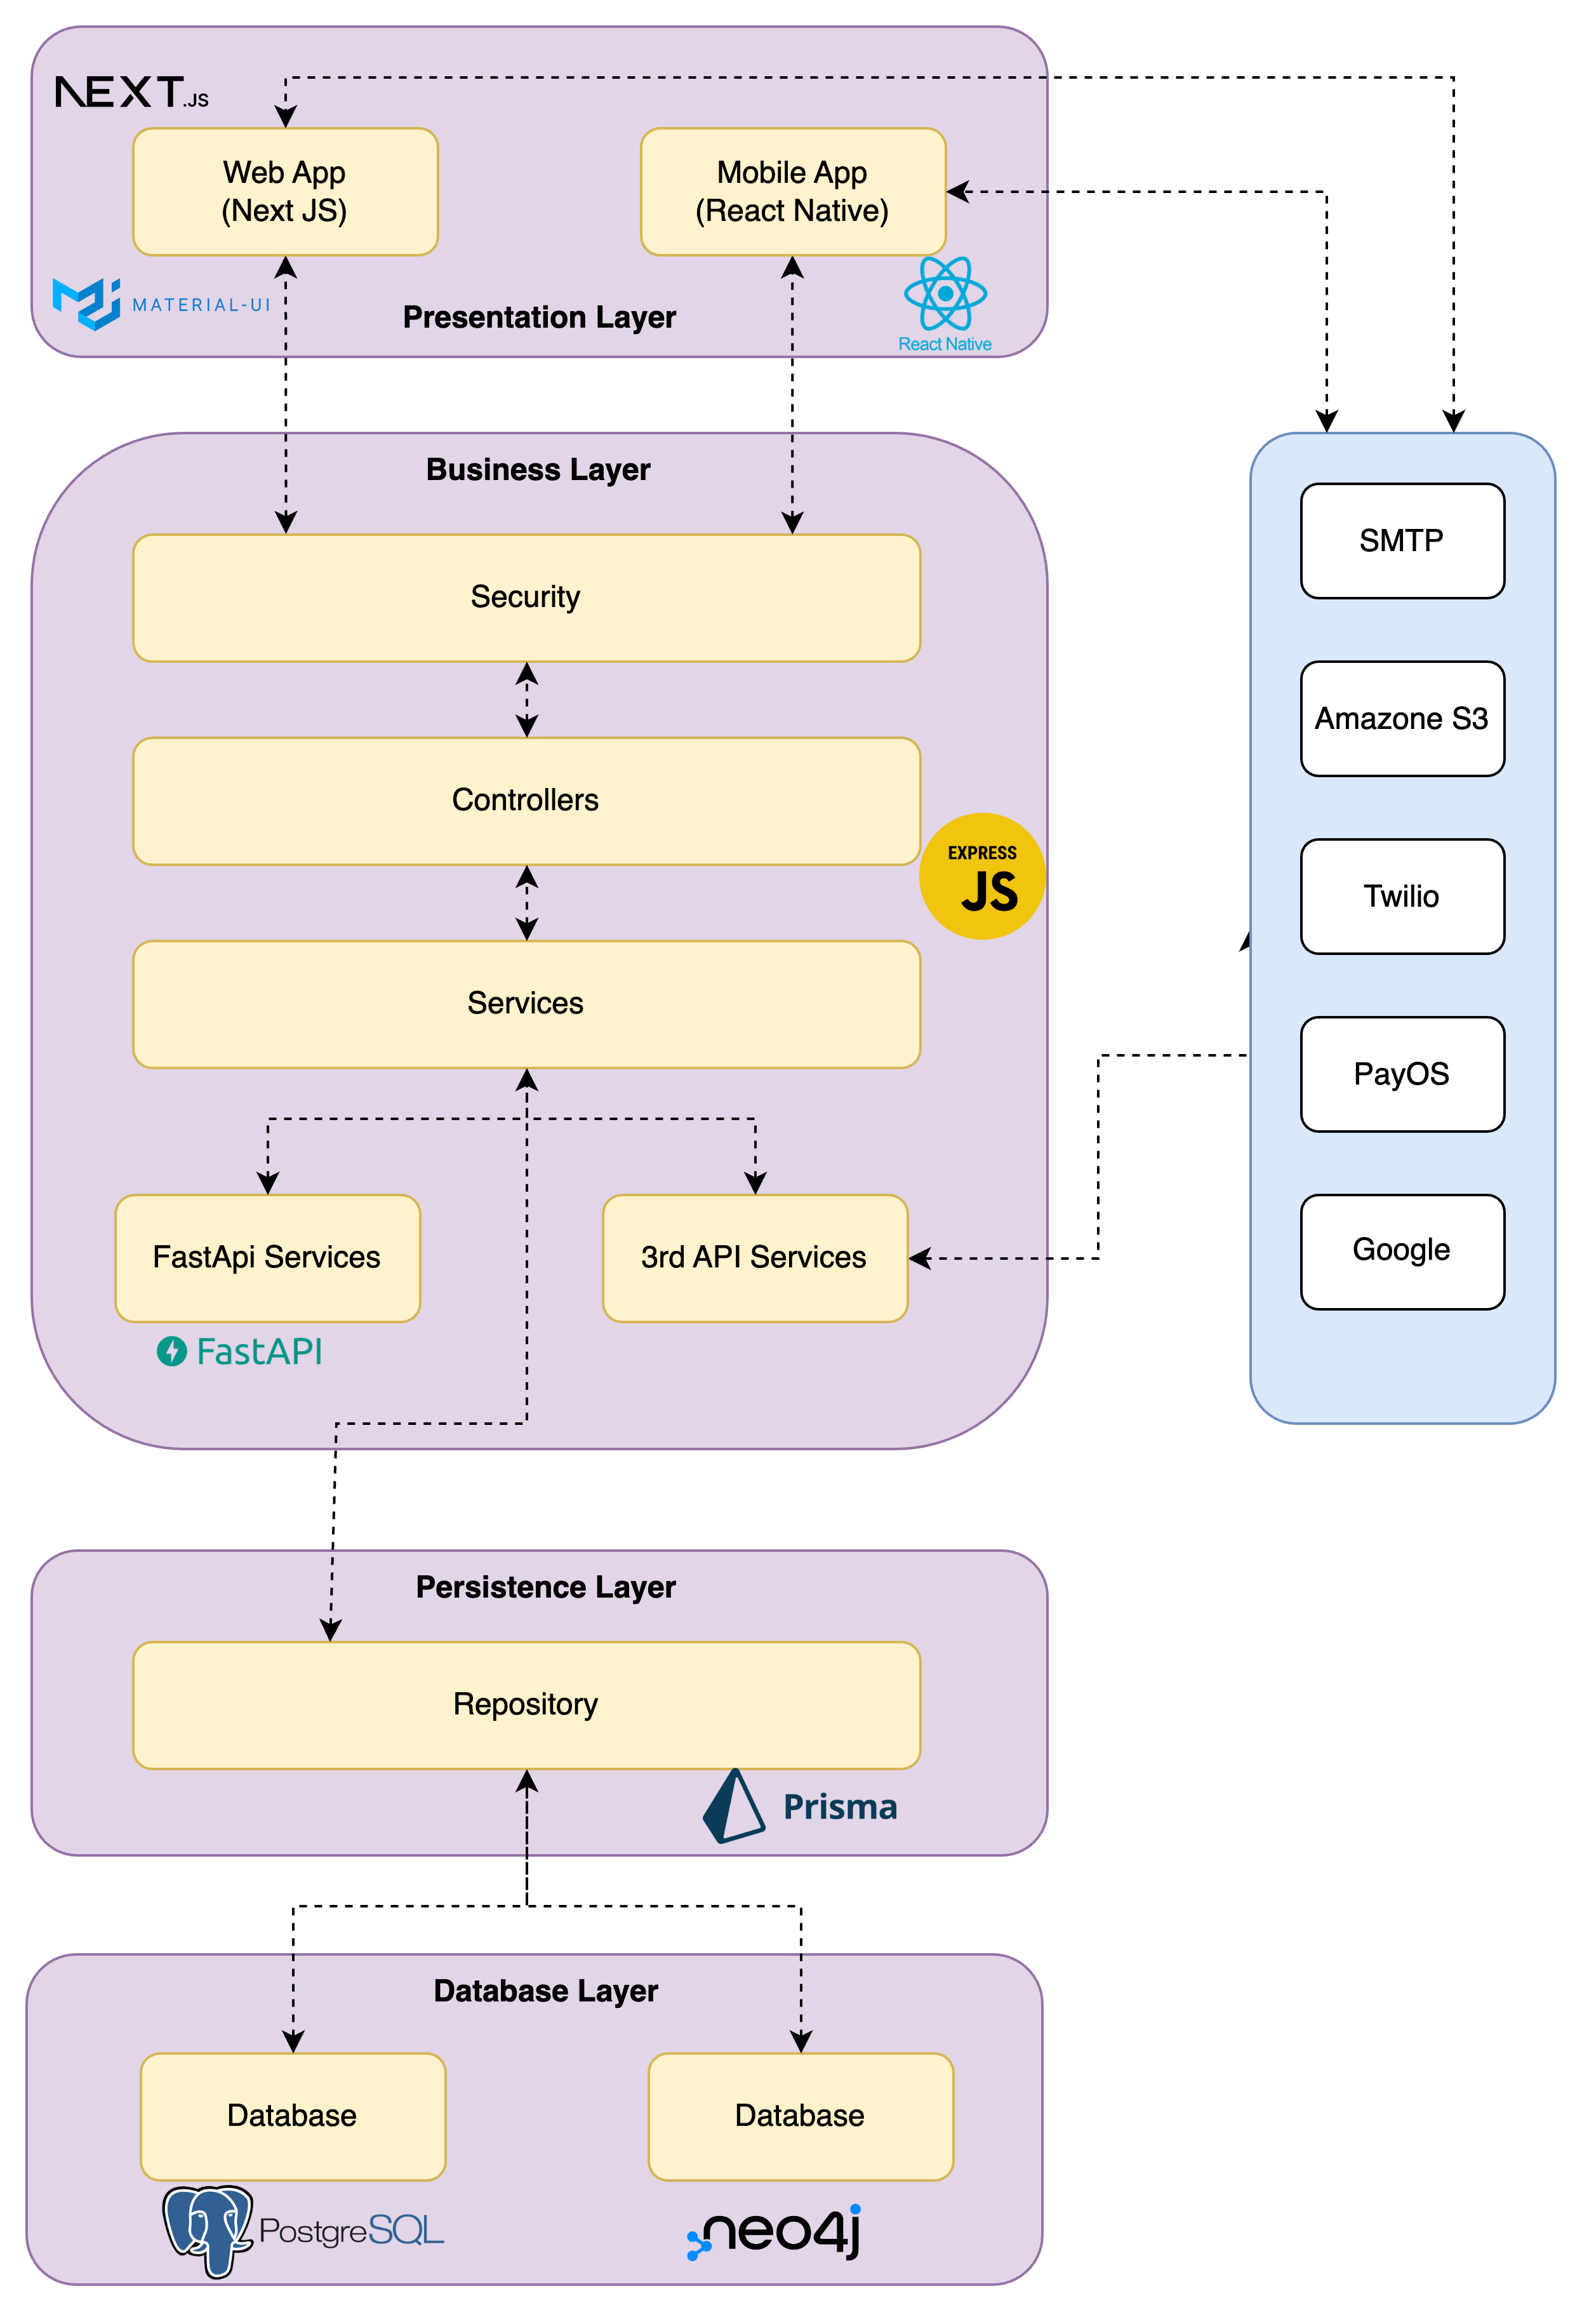
\includegraphics[width=13cm]{Images/architure_system.png}
    \vspace{1cm}
    \caption{Kiến trúc tổng quan của hệ thống}
    \label{fig:enter-label}
\end{figure}
\subsection{Thiết kế cơ sở dữ liệu}
\subsubsection{Thiết kế cơ sở dữ liệu ý niệm}
\begin{figure}[H]
            \centering
            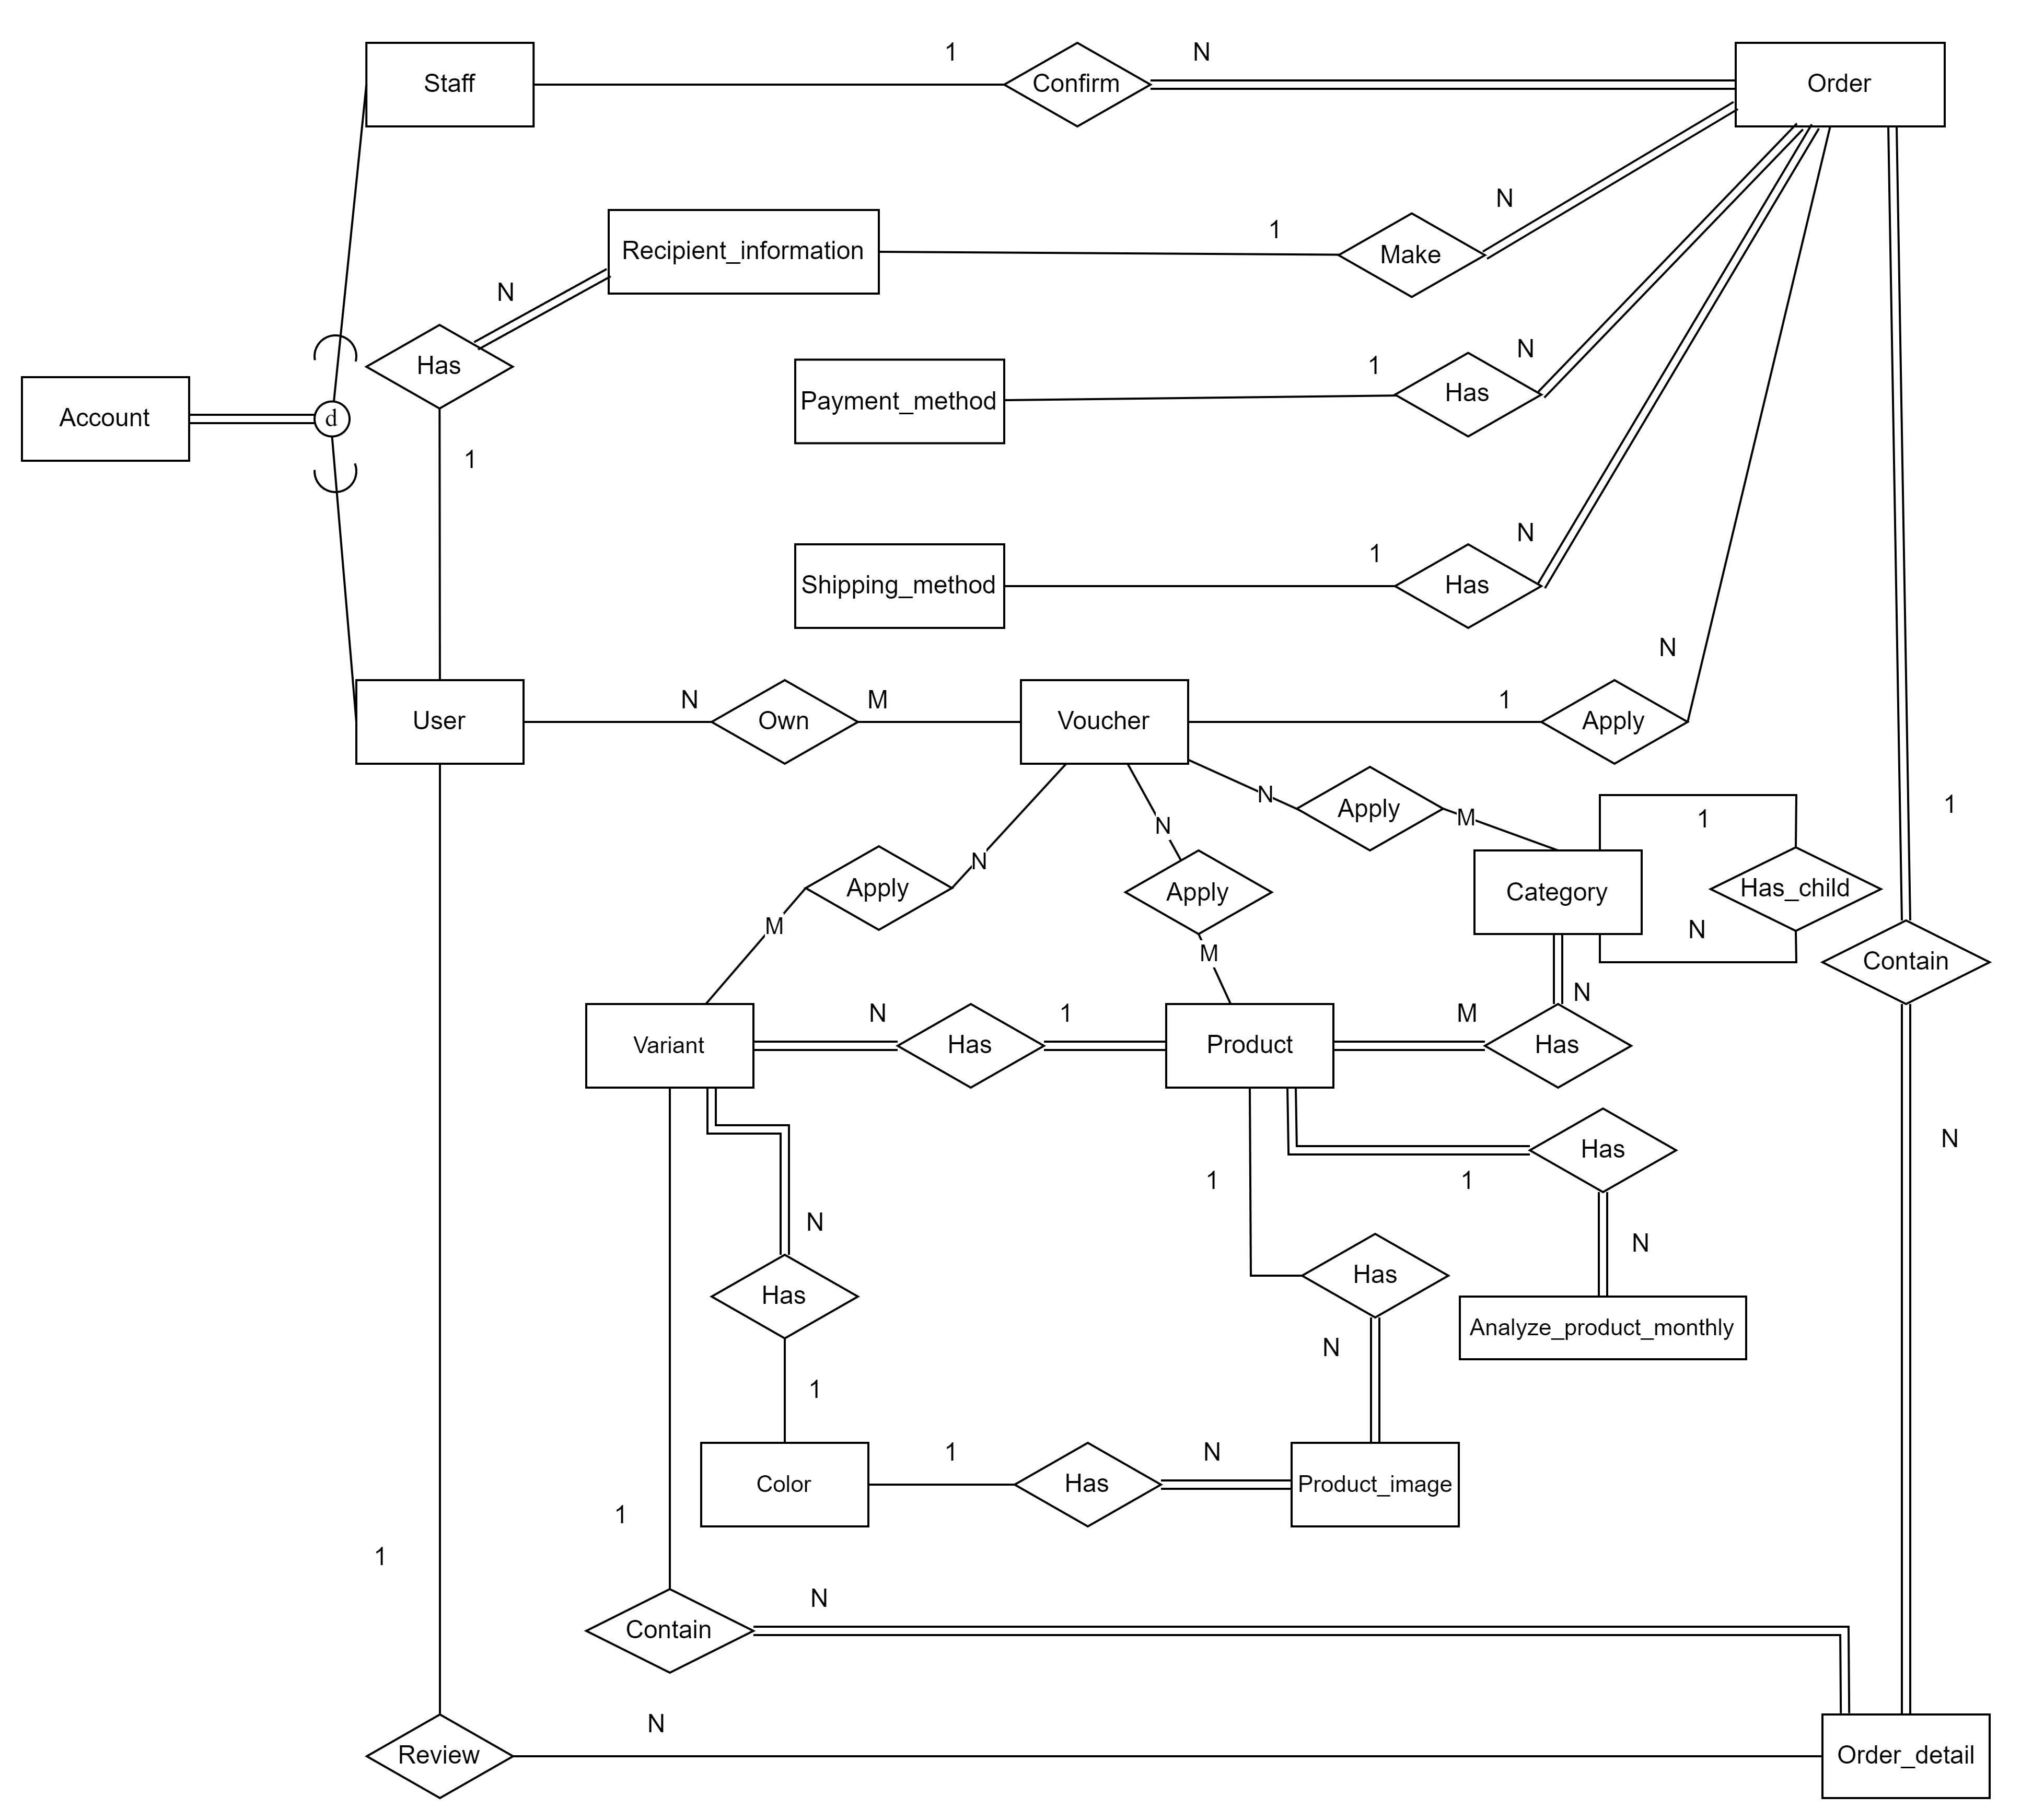
\includegraphics[width=15cm]{Images/ERD/ERD.png}
            \newline
            \newline
            \caption{Thiết kế tổng quan cơ sở dữ liệu ý niệm của cửa hàng thời trang}
            \label{fig:enter-label}
        \end{figure}
%     Các ràng buộc về quan hệ giữa các thực thể:\\
% \begin{itemize}
% \item Một user có thể có nhiều userInfo
% \item Một user có thể sở hữu nhiều voucher
% \item Một user chỉ có một cart
% \item Một user có thể viết nhiều bài review 
% \item Một voucher có thể được sở hữu bởi nhiều user
% \item Một staff có thể xác nhận nhiều đơn hàng
% \item Một user info có thể tạo nhều đơn hàng
% \item Một order chỉ có một phương thức thanh toán
% \item Một order chỉ có một phương thức vận chuyển
% \item Một đơn hàng có thể chứa nhiều đơn hàng chi tiết
% \item 
% \item 
% \item 
% \item 
% \item 
% \end{itemize}
\begin{figure}[H]
            \centering
            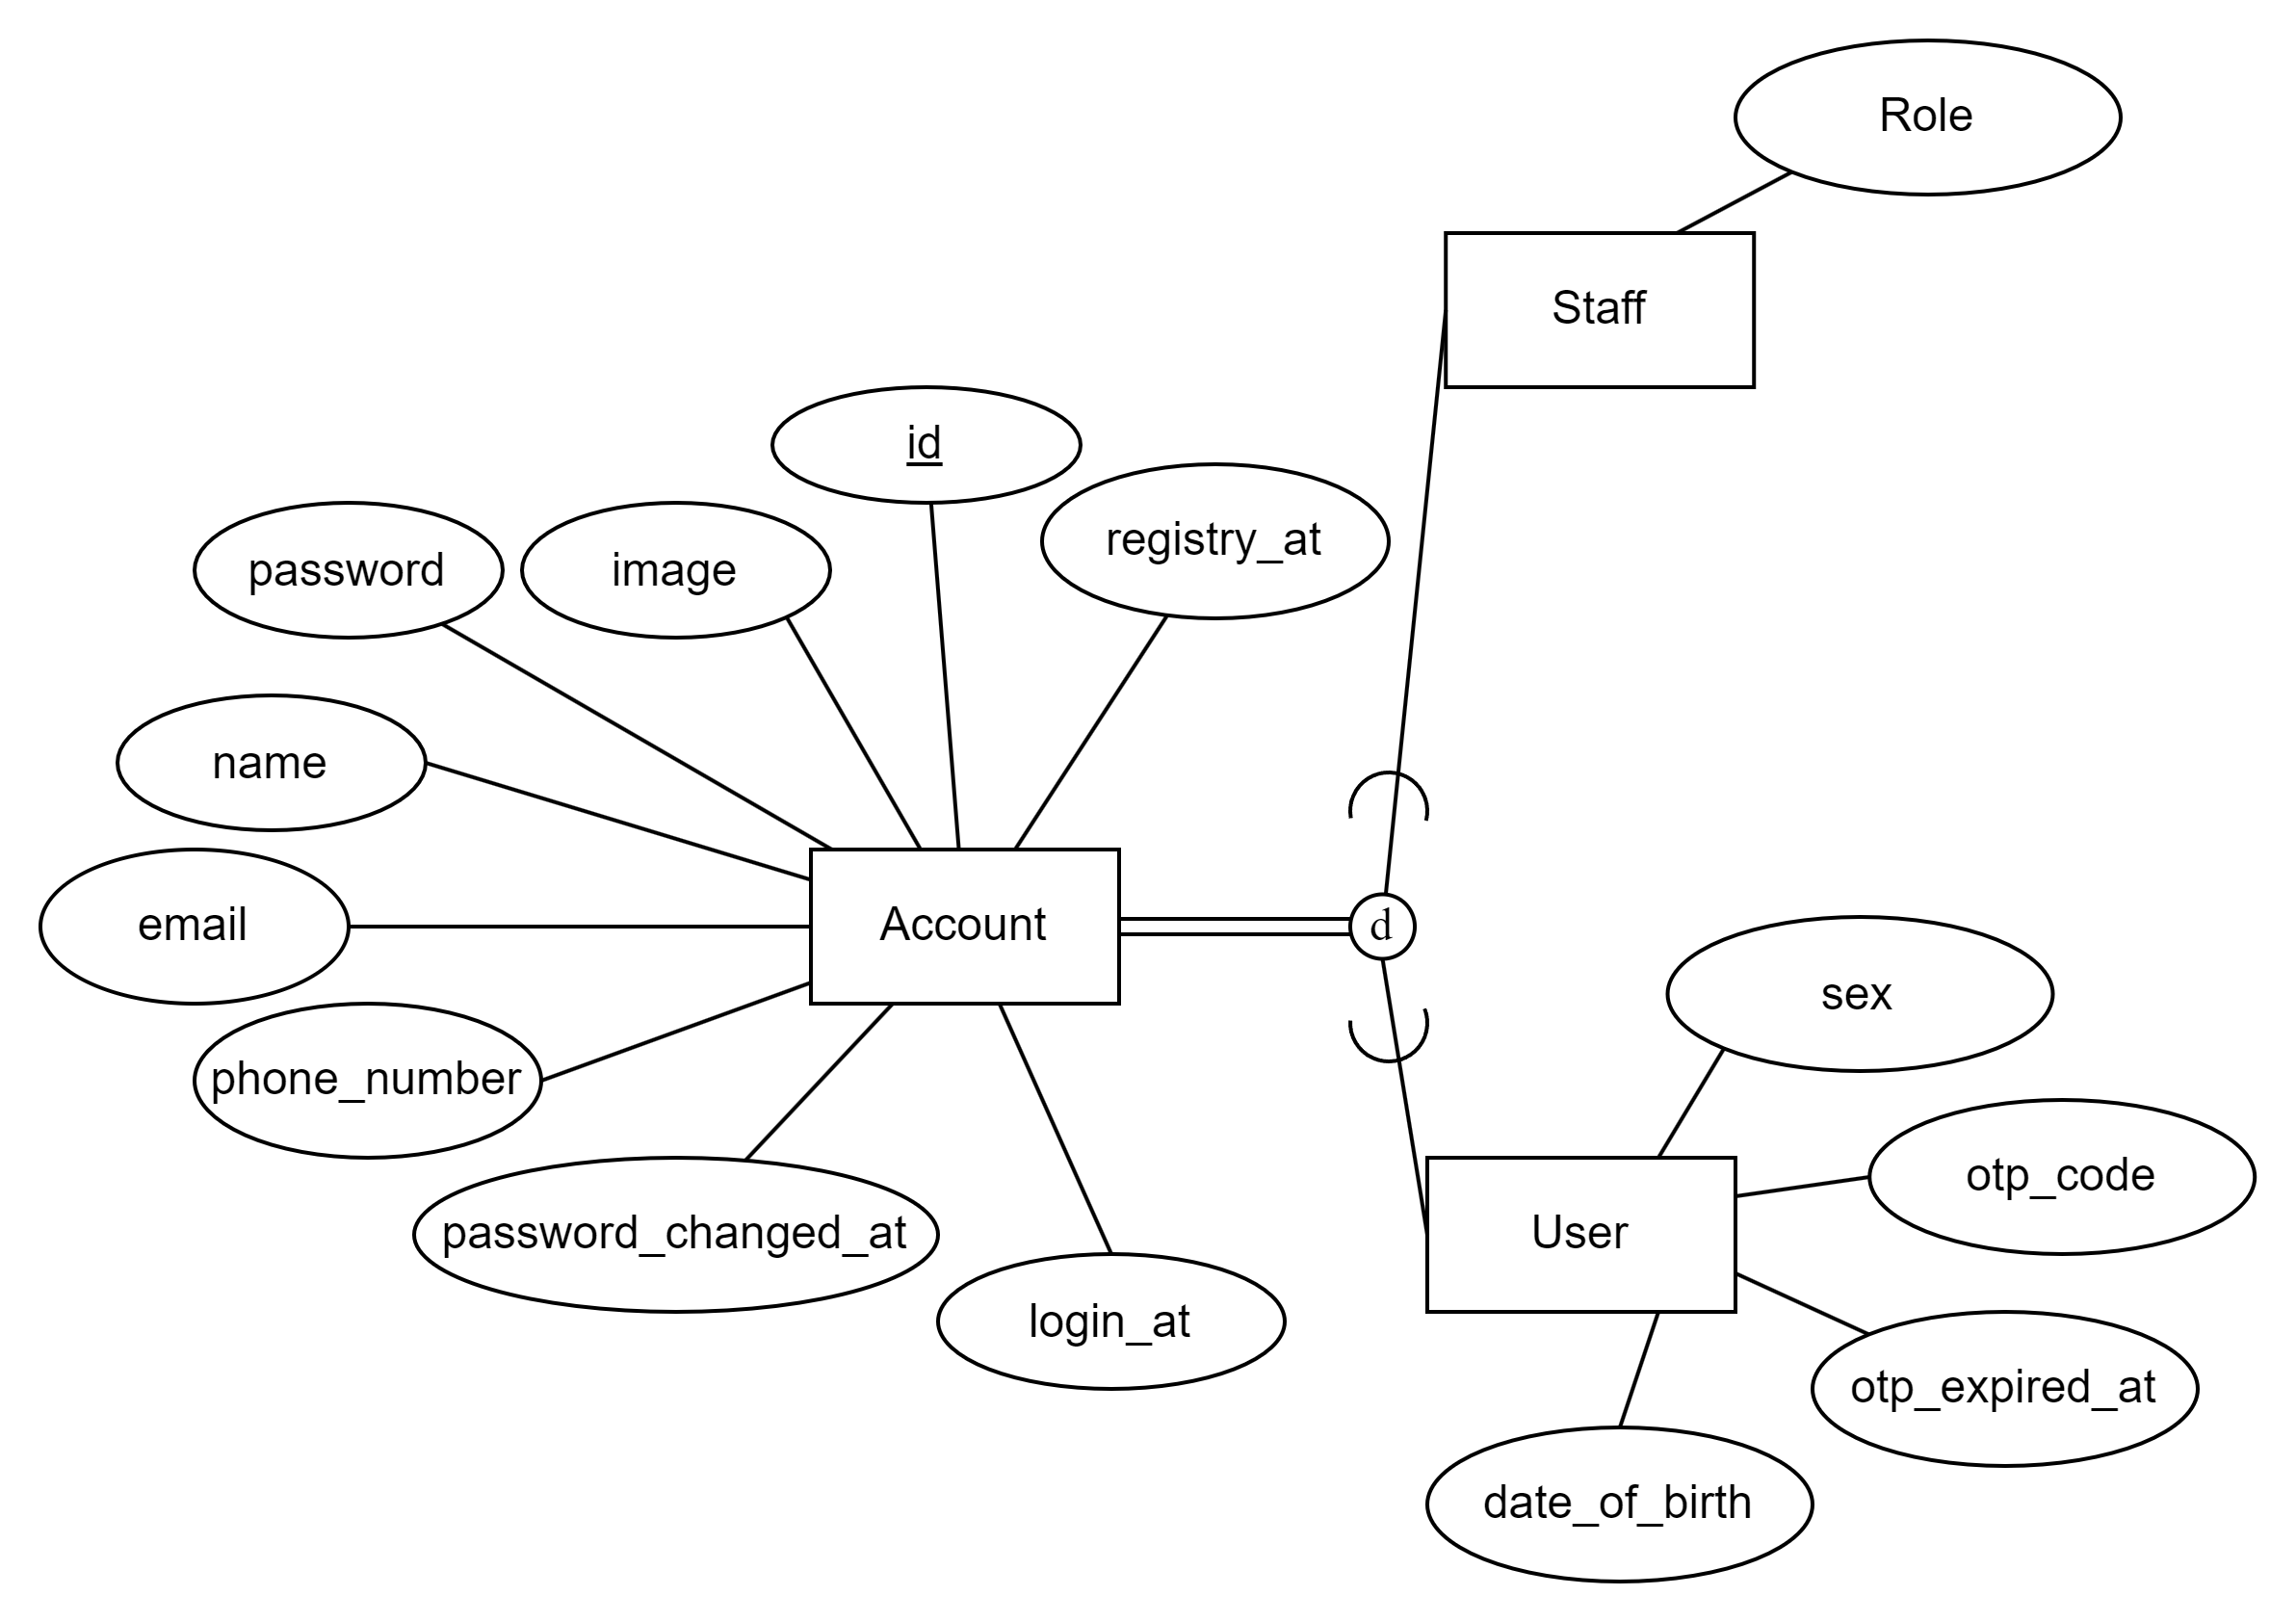
\includegraphics[width=15cm]{Images/ERD/account.png}
            \newline
            \caption{Chi tiết thiết kế của thực thể Account}
            \label{fig:enter-label}
        \end{figure}
        
Các thuộc tính của thực thể Account:
\begin{itemize}
    \item id: Khóa chính, dùng để định danh tài khoản
    \item image: Ảnh đại diện của tài khoản 
\item name: Tên đầy đủ của tài khoản 
\item email: Email của tài khoản 
\item phone number: Số điện thoại của tài khoản
\item password: Mật khẩu của tài khoản
\item password change at: Thời gian gần nhất mà mật khẩu được thay đổi
\item login at: Thời gian của lần đăng nhập gần nhất
\item registry at: Thời gian mà tài khoản được tạo
\end{itemize}

\begin{figure}[H]
            \centering
            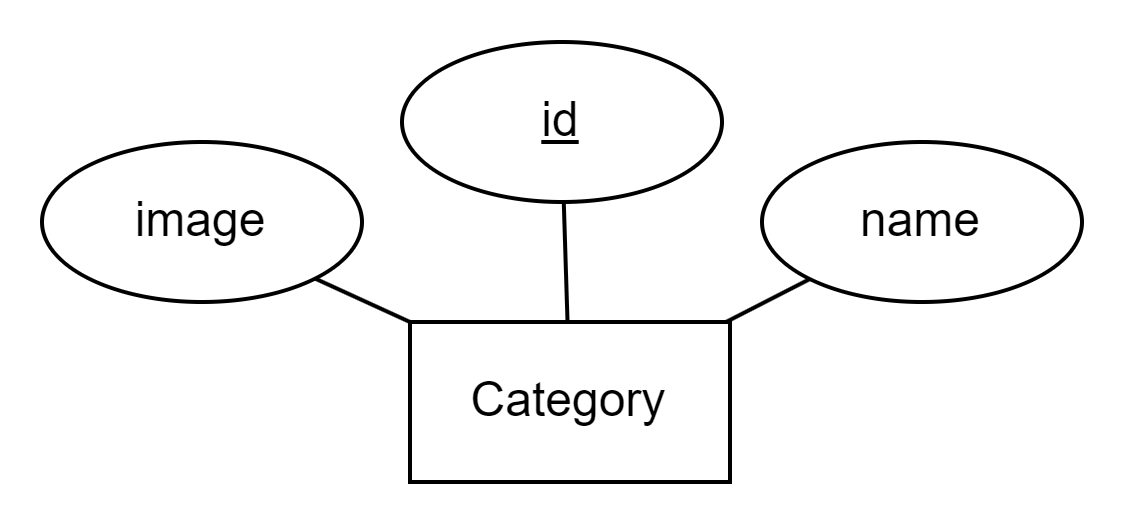
\includegraphics[width=11cm]{Images/ERD/category.png}
            \newline
            \caption{Chi tiết thiết kế của thực thể Category}
            \label{fig:enter-label}
        \end{figure}
        
Các thuộc tính của thực thể Category:
\begin{itemize}
    \item id: Khóa chính, dùng để định danh thể loại/danh mục
    \item name: Tên của thể loại/danh mục
    \item image: Ảnh của thể loại/danh mục
\end{itemize}
% \begin{figure}[H]
%             \centering
%             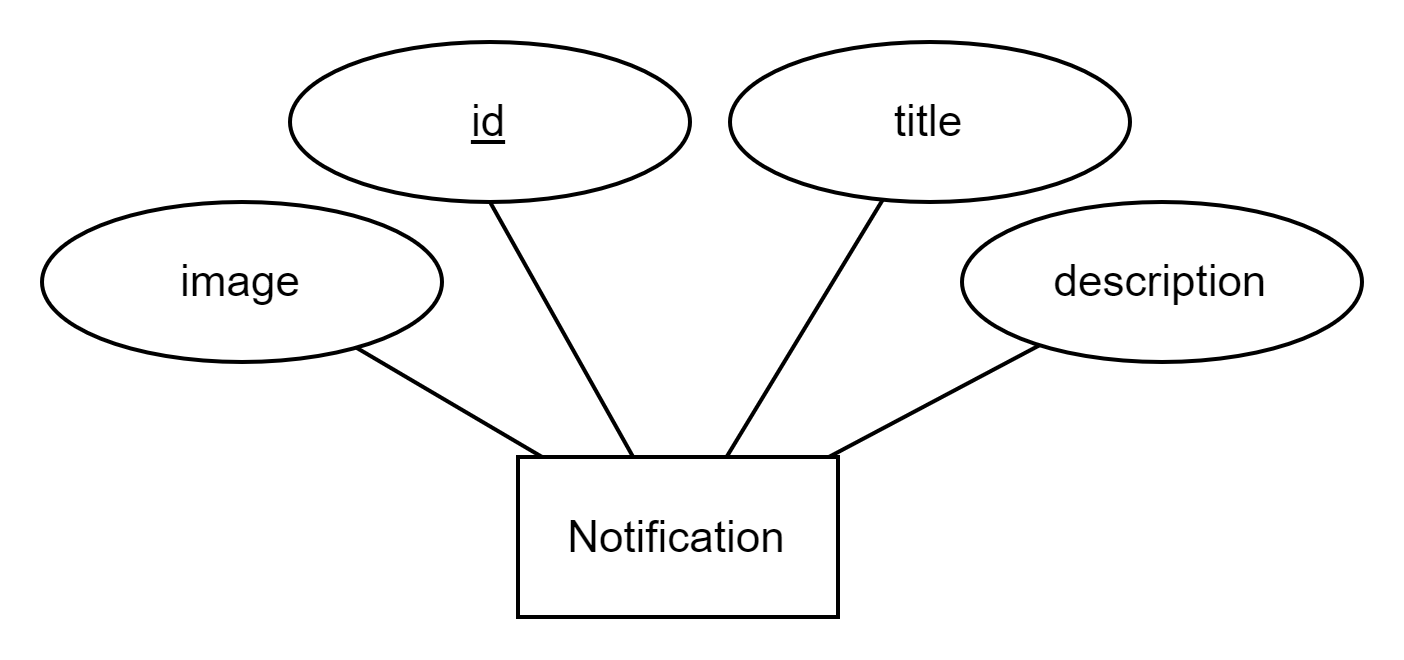
\includegraphics[width=15cm]{Images/ERD/notification.png}
%             \newline
%             \caption{Chi tiết thiết kế của thực thể Notification}
%             \label{fig:enter-label}
%         \end{figure}
% Các thuộc tính của thực thể Notification:
% \begin{itemize}
%     \item id: Khóa chính, dùng để định danh cho thông báo
%     \item title: Tiêu đề của thông báo
%     \item description: Mô tả chi tiết của thông báo
%     \item image: Hình ảnh hiển thị cho thông báo
% \end{itemize}
% \begin{figure}[H]
%             \centering
%             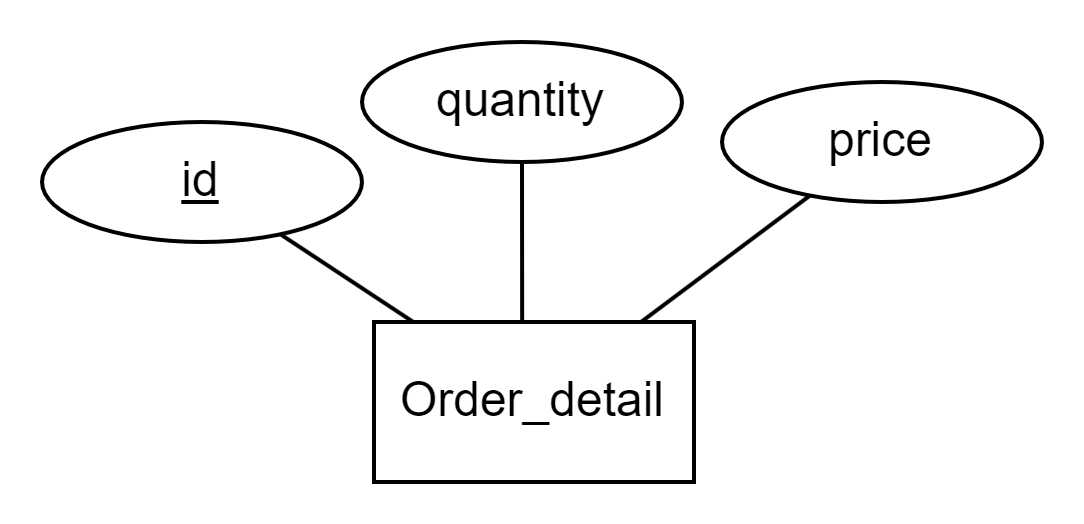
\includegraphics[width=11cm]{Images/ERD/order_detail.png}
%             \newline
%             \caption{Chi tiết thiết kế của thực thể Order Detail}
%             \label{fig:enter-label}
%         \end{figure}
% Các thuộc tính của thực thể Order Detail:
% \begin{itemize}
%     \item id: Khóa chính, dùng để định danh cho đơn hàng chi tiết
%     \item quantity: Số lượng sản phẩm trong đơn hàng chi tiết
% \end{itemize}
\begin{figure}[H]
            \centering
            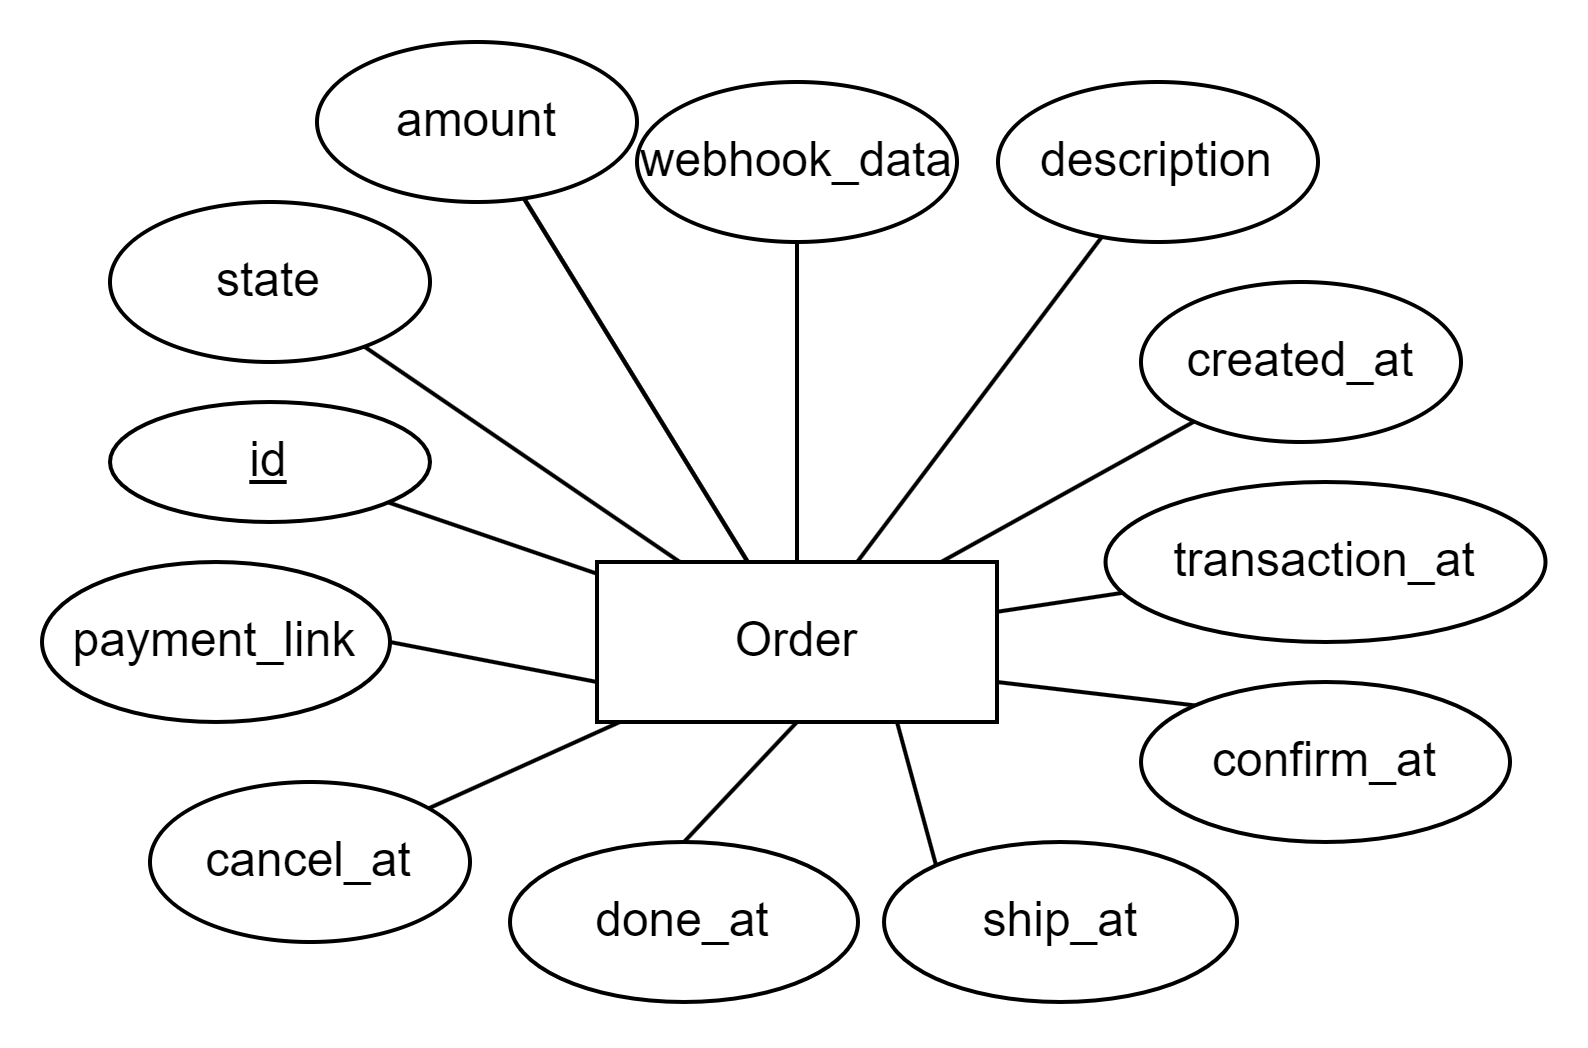
\includegraphics[width=15cm]{Images/ERD/order.png}
            \newline
            \caption{Chi tiết thiết kế của thực thể Order}
            \label{fig:enter-label}
        \end{figure}

\newpage       
Các thuộc tính của thực thể Order:
\begin{itemize}
    \item id: Khóa chính, dùng để định danh cho mỗi đơn hàng
    \item state: Trạng thái của đơn hàng
    \item amount: Tổng tiền của đơn hàng
    \item description: Mô tả chi tiết của đơn hàng
    \item create at: Thời gian đơn hàng được tạo
    \item transaction when: Thời điểm thanh toán
    \item webhook data: Thông tin thanh toán
    \item confirm at: Thời điểm đơn hàng được chấp thuận từ staff
    \item ship at: Thời điểm đơn hàng tiến hành vận chuyển
    \item done at: Thời điểm đơn hàng hoàn thành
    \item cancel at: Thời điểm đơn hàng bị hủy
    \item payment link: Đường dẫn thanh toán điện tử
\end{itemize}
\begin{figure}[H]
            \centering
            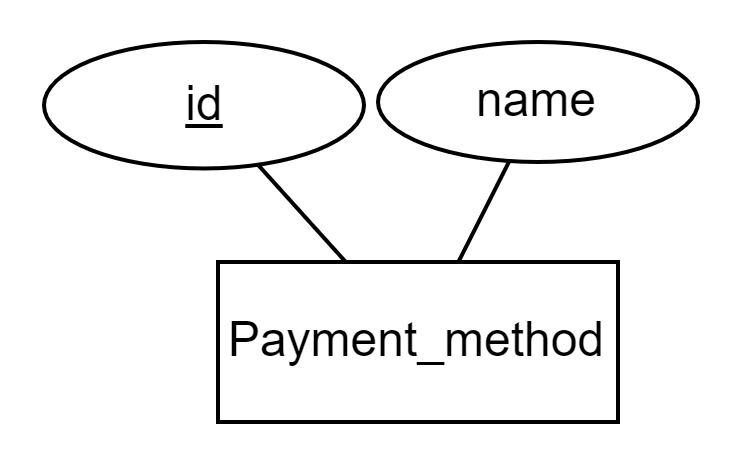
\includegraphics[width=10cm]{Images/ERD/payment_method.png}
            \newline
            \caption{Chi tiết thiết kế của thực thể Payment Method}
            \label{fig:enter-label}
        \end{figure}
        
Các thuộc tính của thực thể Payment Method:
\begin{itemize}
    \item id: Khóa chính, dùng để định danh cho mỗi phương thức thanh toán
    \item name: Tên của phương thức thanh toán
\end{itemize}
\begin{figure}[H]
            \centering
            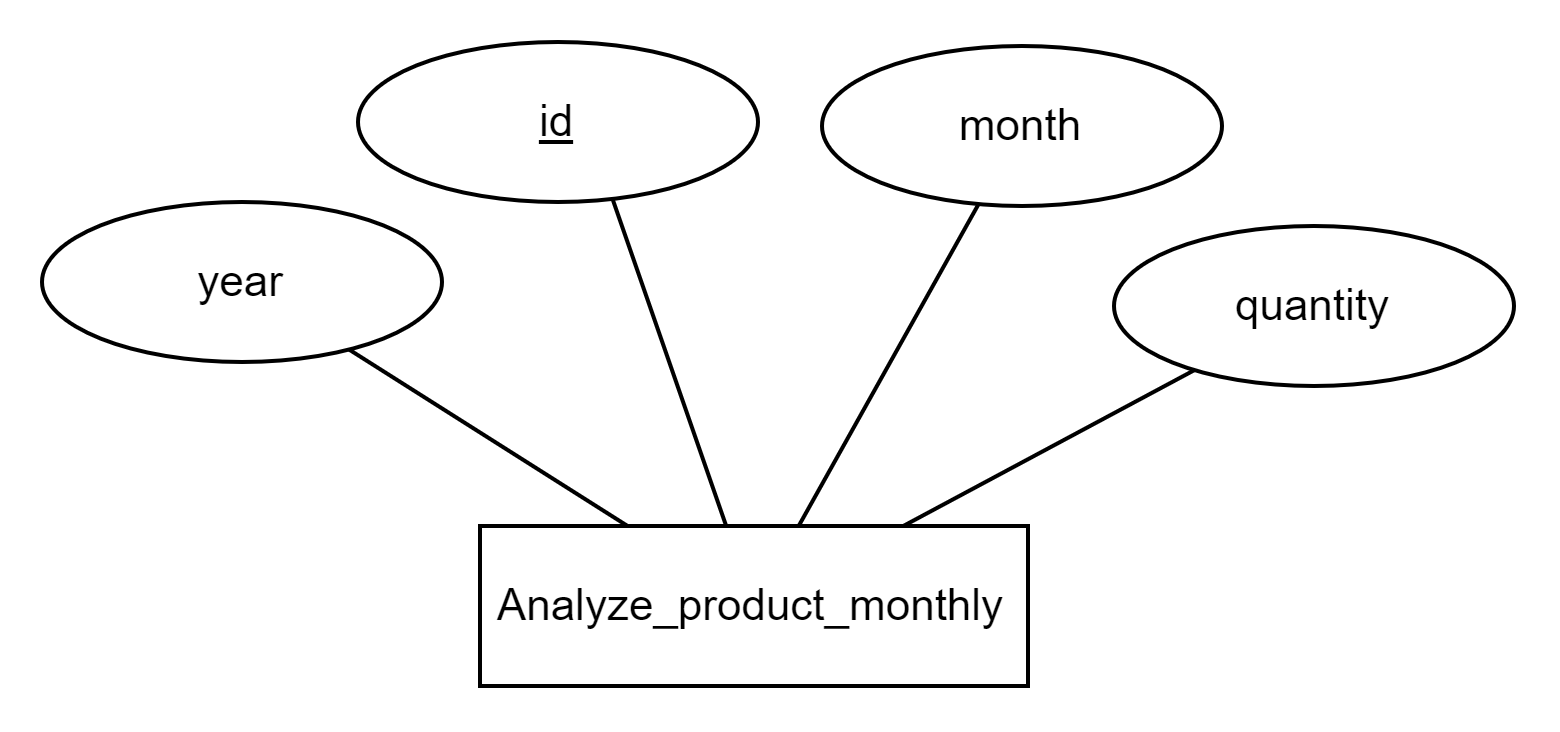
\includegraphics[width=15cm]{Images/ERD/product_bought.png}
            \newline
            \caption{Chi tiết thiết kế của thực thể Analyze product monthly}
            \label{fig:enter-label}
        \end{figure}
Các thuộc tính của thực thể Analyze product monthly:
\begin{itemize}
    \item id: Khóa chính, dùng để định danh cho mỗi sản phẩm bán chạy
    \item month: Sản phẩm bán chạy trong tháng n
    \item year: Sản phẩm bán chạy trong năm m
    \item quantity: Số lượng sản phẩm đó được bán ra trong tháng-năm đó
\end{itemize}
\begin{figure}[H]
            \centering
            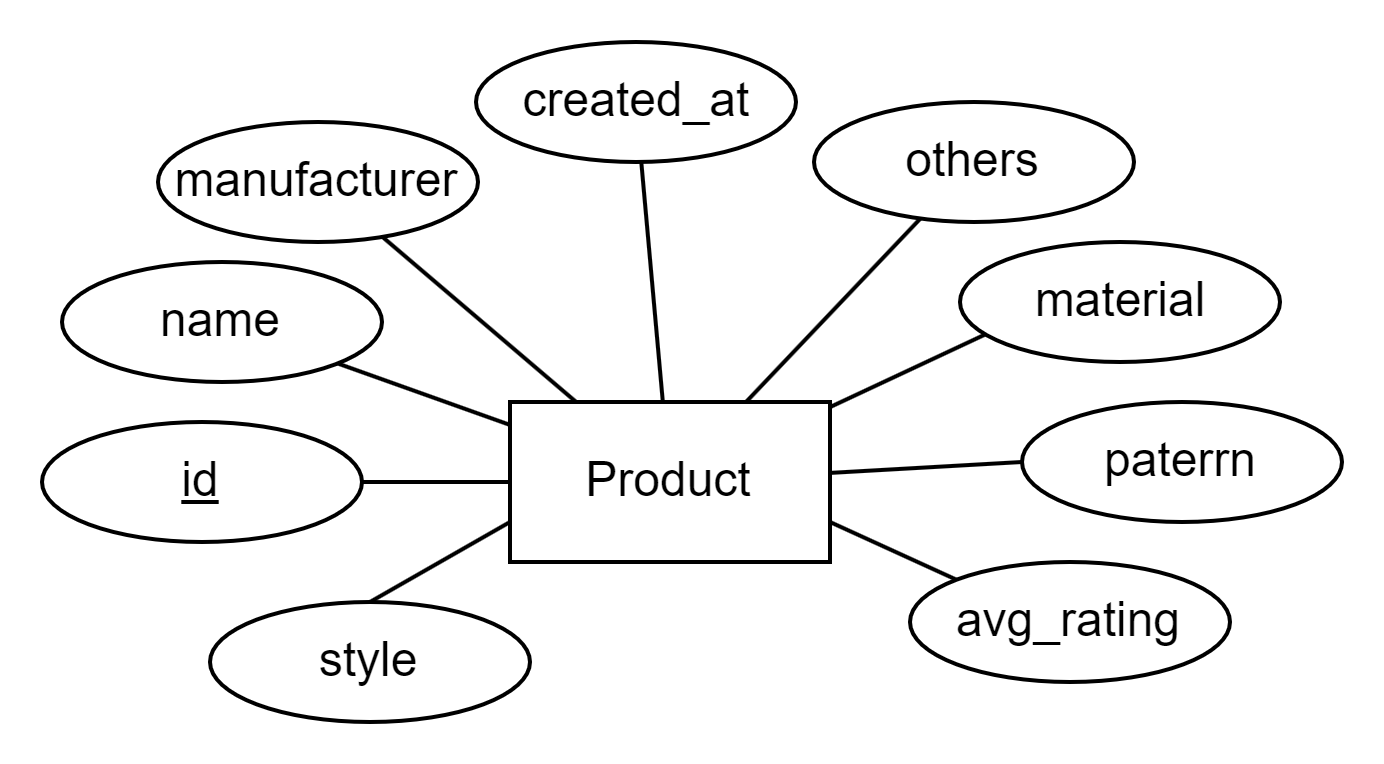
\includegraphics[width=15cm]{Images/ERD/product.png}
            \newline
            \caption{Chi tiết thiết kế của thực thể Product}
            \label{fig:enter-label}
        \end{figure}

\newpage
Các thuộc tính của thực thể Product:
\begin{itemize}
    \item id: Khóa chính, dùng để định danh cho mỗi sản phẩm
    \item name: Tên sản phẩm
    \item manufacturer: Tên nhà sản xuất cho sản phẩm đó
    \item create at: Ngày sản phẩm được thêm vào hệ thống
    \item others: Mô tả cho sản phẩm
    \item material: Chất liệu của sản phẩm
    \item pattern: Họa tiết sản phẩm
    \item style: Phong cách của sản phẩm
    \item avg rating: Đánh giá trung bình của sản phẩm
\end{itemize}
% \begin{figure}[H]
%             \centering
%             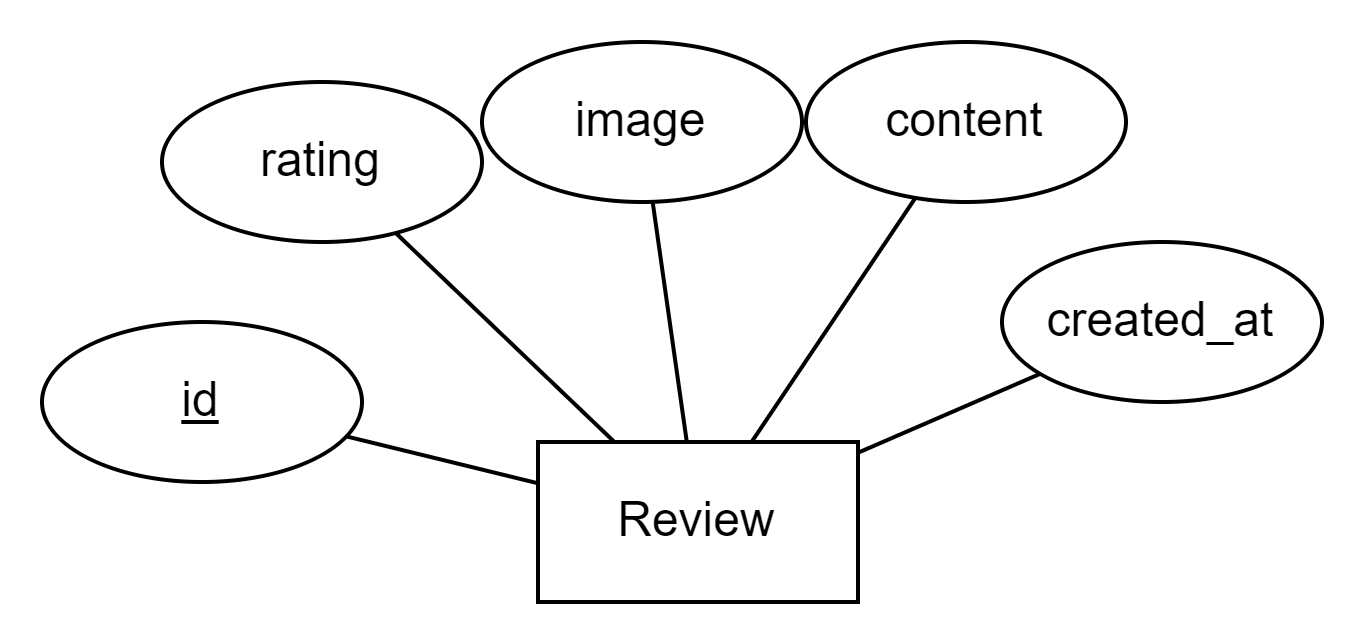
\includegraphics[width=15cm]{Images/ERD/review.png}
%             \newline
%             \caption{Chi tiết thiết kế của thực thể Review}
%             \label{fig:enter-label}
%         \end{figure}
% Các thuộc tính của thực thể Review:
% \begin{itemize}
%     \item id: Khóa chính, dùng để định danh cho mỗi bài đánh giá sản phẩm
%     \item rating: Số sao danh của bài viết đánh giá cho sản phẩm
%     \item content: Nội dung của bài đánh giá
%     \item create at: Ngày mà bài đánh giá được người dùng tạo trên hệ thống
%     \item image: Hình ảnh của người dùng tải lên cho bài đánh giá
% \end{itemize}
\begin{figure}[H]
            \centering
            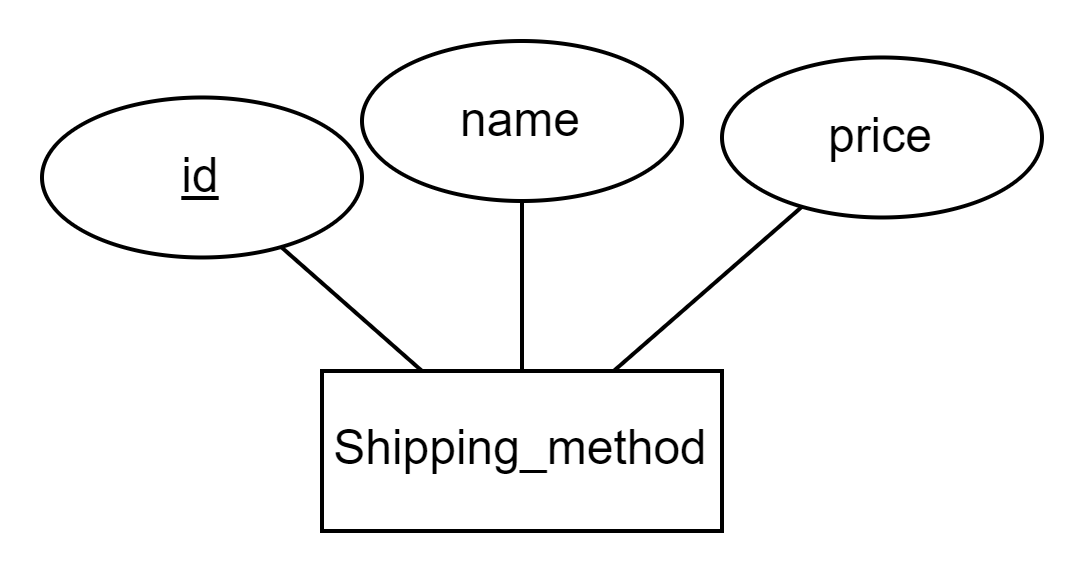
\includegraphics[width=13cm]{Images/ERD/shipping_method.png}
            \newline
            \caption{Chi tiết thiết kế của thực thể Shipping Method}
            \label{fig:enter-label}
        \end{figure}
Các thuộc tính của thực thể Shipping Method:
\begin{itemize}
    \item id: Khóa chính, dùng để định danh cho mỗi phương thức vận chuyển
    \item name: Tên phương thức vận chuyển
    \item price: Giá vận chuyển của phương thức vận chuyển đó
\end{itemize}
\begin{figure}[H]
            \centering
            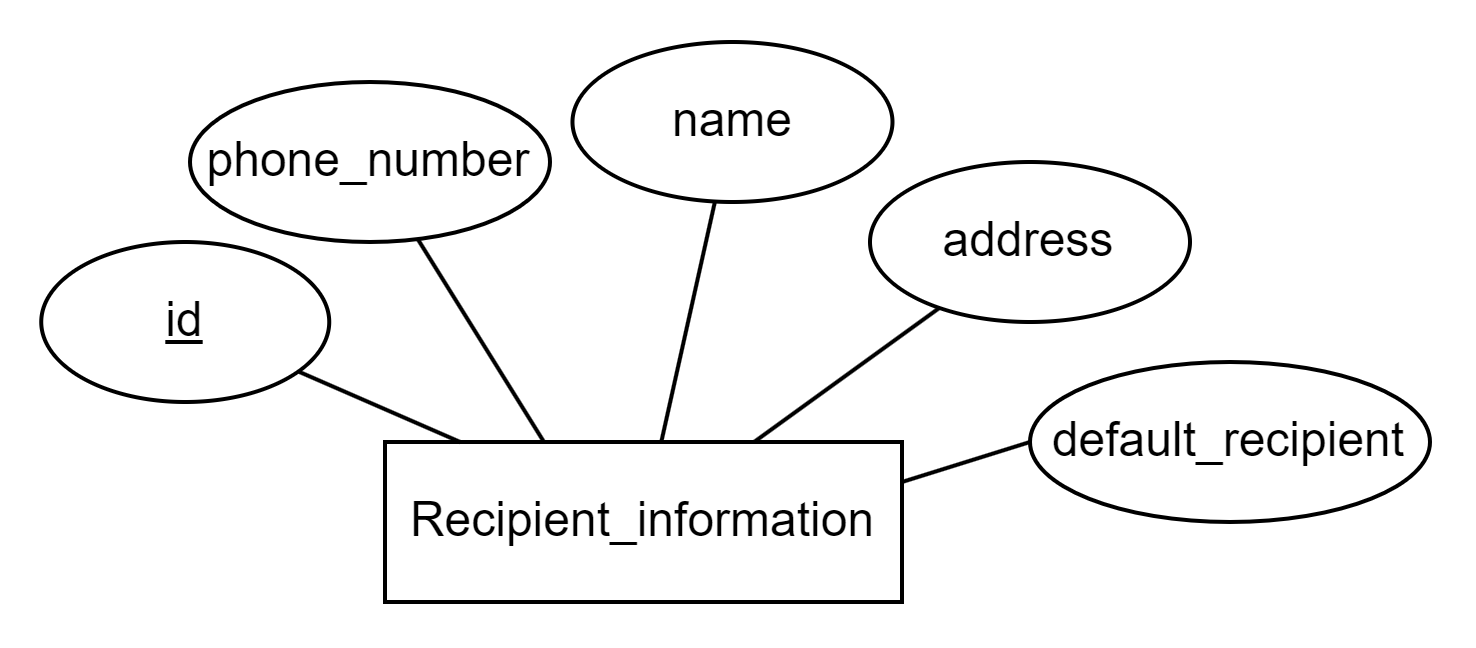
\includegraphics[width=15cm]{Images/ERD/user_info.png}
            \newline
            \caption{Chi tiết thiết kế của thực thể Recipient information}
            \label{fig:enter-label}
        \end{figure}

Các thuộc tính của thực thể Recipient information:
\begin{itemize}
    \item id: Khóa chính, dùng để định danh cho mỗi Thông tin người dùng
    \item address: Địa chỉ nhận hàng của người dùng
    \item name: Tên của người nhận hàng
    \item phone number: Số điện thoại của người nhận hàng
    \item default recipient: Thiết lập thông tin nhận hàng mặc định
\end{itemize}
\begin{figure}[H]
            \centering
            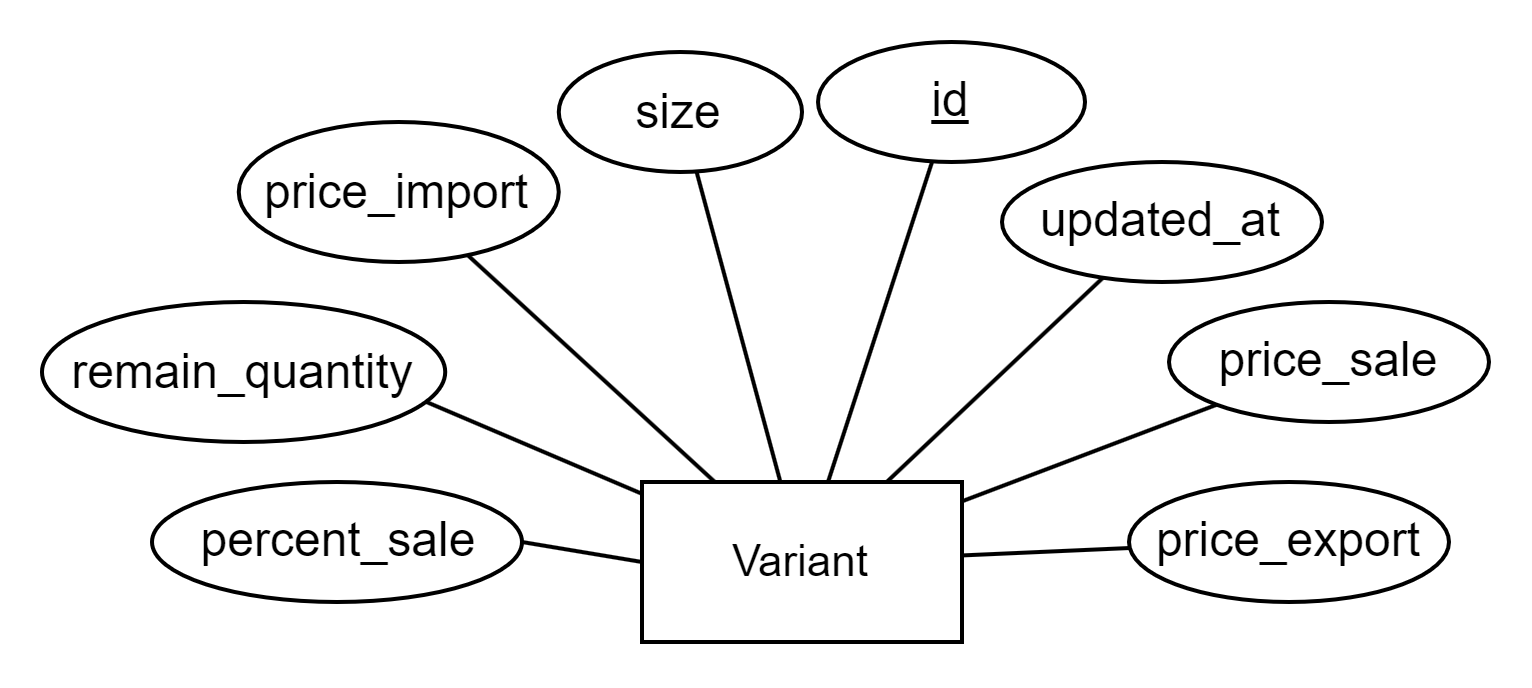
\includegraphics[width=15cm]{Images/ERD/variant.png}
            \newline
            \caption{Chi tiết thiết kế của thực thể Variant}
            \label{fig:enter-label}
        \end{figure}

\newpage
Các thuộc tính của thực thể Variant:
\begin{itemize}
\item id: Khóa chính, dùng để định danh cho mỗi biến sản phẩm
\item size: Kích cỡ của sản phẩm
\item price import: Giá nhập vào của sản phẩm
\item price sale: Giá của sản phẩm sau khi được giảm giá
\item remain quantity: Số lượng còn lại của sản phẩm
\item price export: Giá bán của sản phẩm
\item update at: Thời gian gần nhất sản phẩm được cập nhật
\item percent sale: Phần trăm giảm giá của sản phẩm
\end{itemize}
\begin{figure}[H]
            \centering
            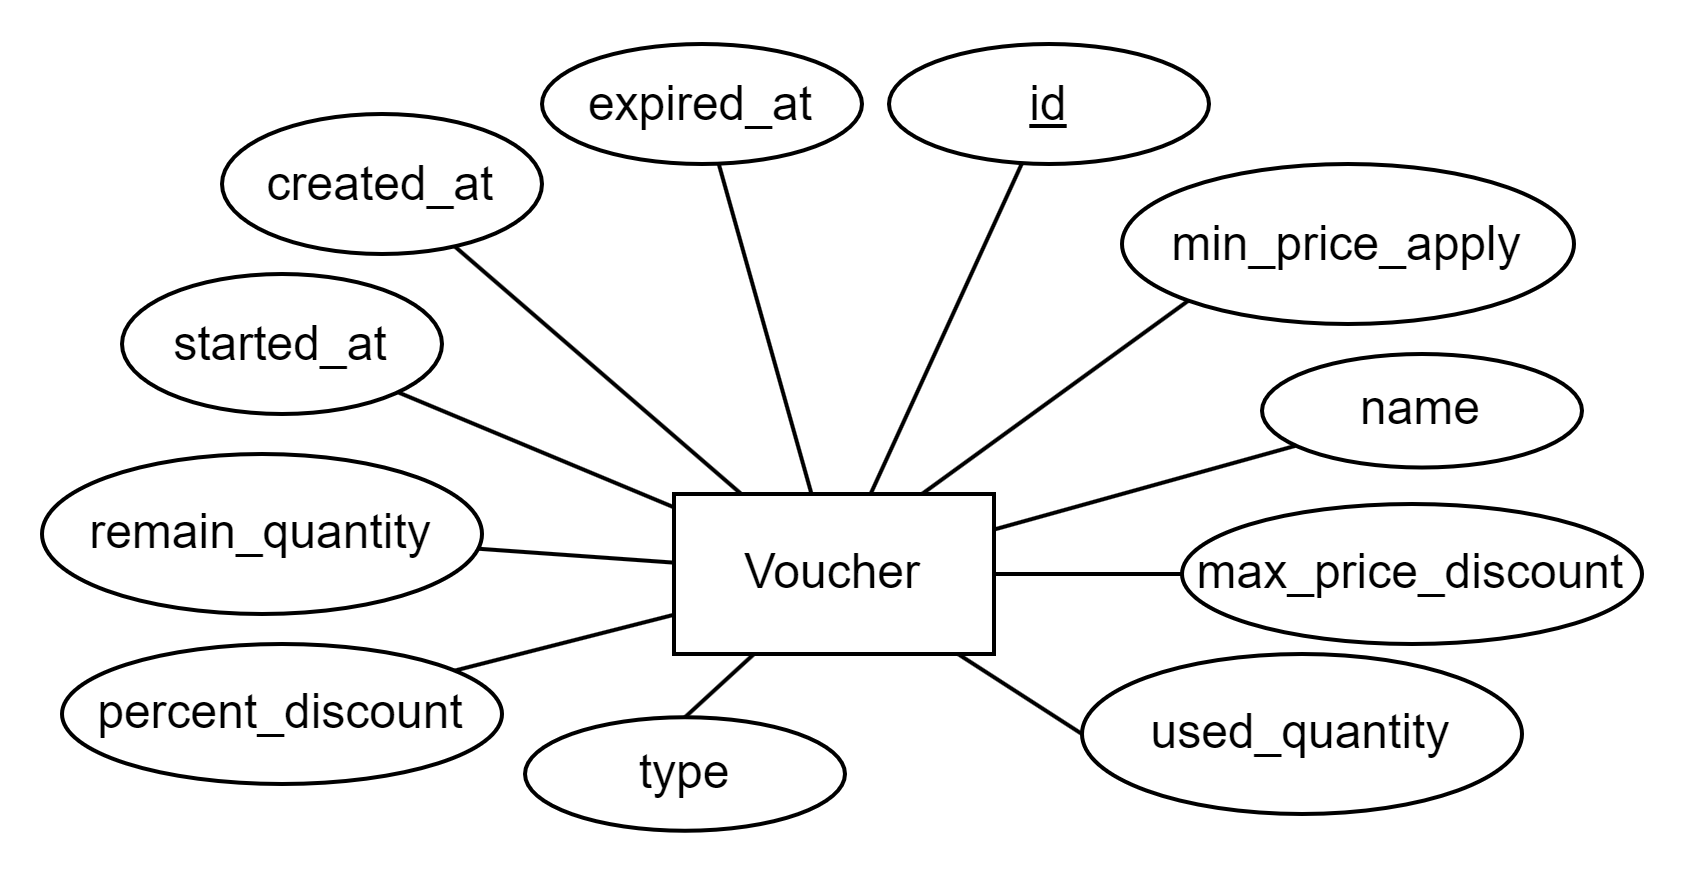
\includegraphics[width=15cm]{Images/ERD/voucher.png}
            \newline
            \caption{Chi tiết thiết kế của thực thể Voucher}
            \label{fig:enter-label}
\end{figure}
Các thuộc tính của thực thể Voucher:
\begin{itemize}
\item id: Khóa chính, dùng để định danh cho mỗi mã giảm giá
\item name: Tên của mã giảm giá
\item expire at: Ngày hết hạn của mã giảm giá
\item create at: Ngày tạo mã giảm giá
\item started at: Ngày bắt đầu có hiệu lực của mã giảm giá
\item remain quantity: Số lượng còn lại của mã giảm giá
\item percent discount: Phần trăm giảm giá của voucher
\item min price apply: Số tiền tối thiểu để có thể áp dụng voucher
\item max price discount: Số tiền tối đa có thể được giảm từ voucher 
\item type: Loại hình voucher
\item used quantity: số lượng voucher đã được sử dụng
\end{itemize}

\begin{figure}[H]
            \centering
            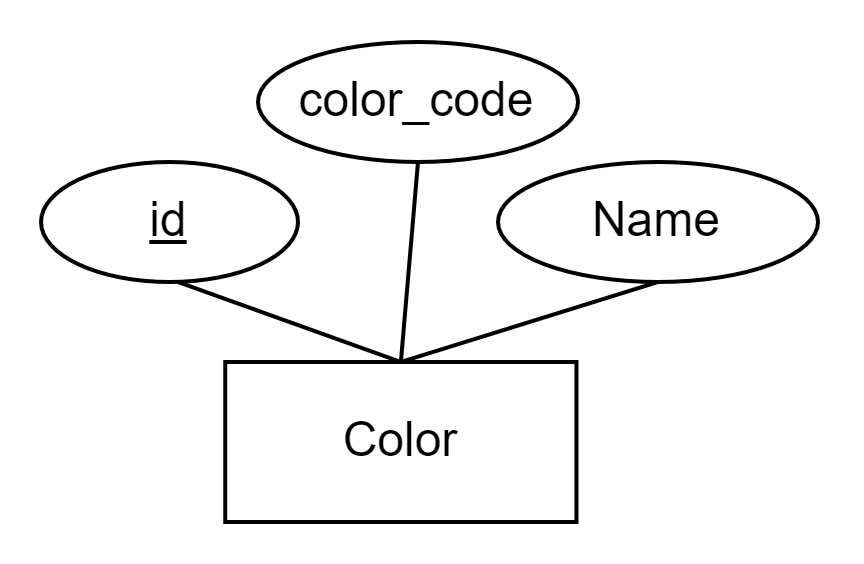
\includegraphics[width=11cm]{Images/ERD/color.png}
            \newline
            \caption{Chi tiết thiết kế của thực thể Color}
            \label{fig:enter-label}
\end{figure}
Các thuộc tính của thực thể Color:
\begin{itemize}
\item id: Khóa chính, dùng để định danh cho mỗi màu sắc
\item name: Tên của màu
\item color code: Mãu màu dạng HEX
\end{itemize}
\newpage
\begin{figure}[H]
            \centering
            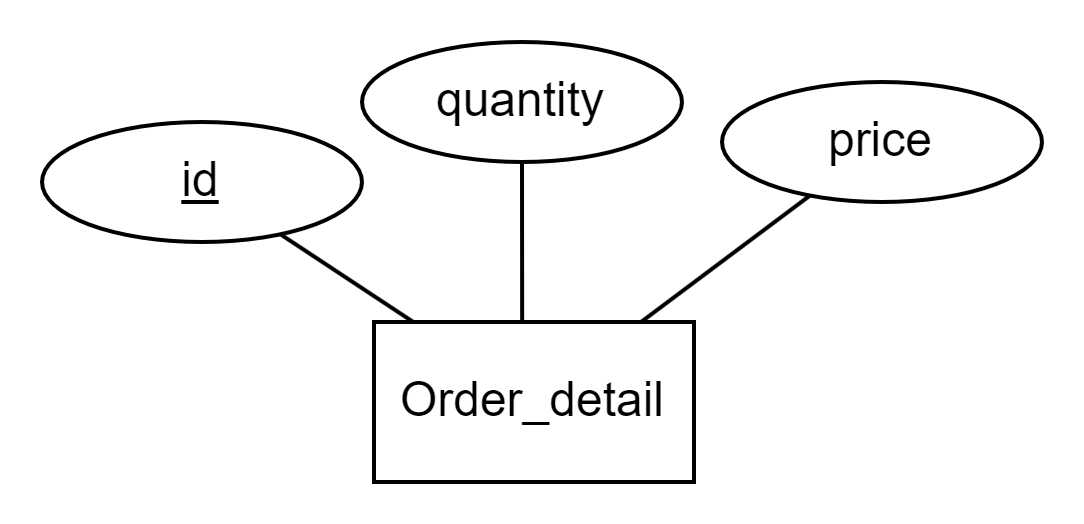
\includegraphics[width=11cm]{Images/ERD/order_detail.png}
            \newline
            \caption{Chi tiết thiết kế của thực thể Order detail}
            \label{fig:enter-label}
\end{figure}
Các thuộc tính của thực thể Order detail:
\begin{itemize}
\item id: Khóa chính, dùng để định danh cho mỗi variant có trong order
\item quantity: Số lượng của variant đó trong đơn hàng
\item price: Giá trị của toàn bộ variant đó trong đơn hàng
\end{itemize}

\begin{figure}[H]
            \centering
            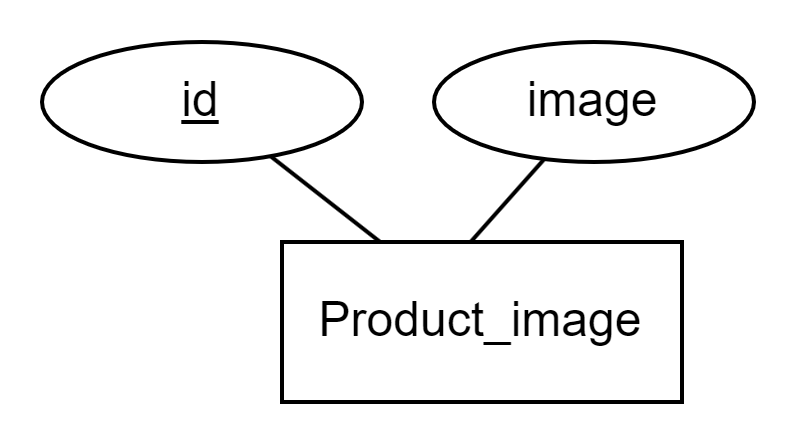
\includegraphics[width=11cm]{Images/ERD/product_image.png}
            \newline
            \caption{Chi tiết thiết kế của thực thể Product image}
            \label{fig:enter-label}
\end{figure}
Các thuộc tính của thực thể Order detail:
\begin{itemize}
\item id: Khóa chính, dùng để định danh cho mỗi ảnh
\item image: Đường dẫn(link) của ảnh đó
\end{itemize}

\newpage
\subsubsection{Thiết kế cơ sở dữ liệu vật lý}
Bảng Staff lưu trữ thông tin của các nhân viên
\begin{table}[H]
\centering
\begin{tabular}{|p{4cm}|p{3cm}|p{7cm}|}
\hline
Thuộc tính & Kiểu dữ liệu & Mô tả \\
\hline
id & integer & Khóa chính \\
\hline
name & varchar &  \\
\hline
email & varchar & \\
\hline
password & varchar & \\
\hline
phone\_number & varchar & \\
\hline
image & varchar & \\
\hline
password\_change\_at & timestamp & \\
\hline
last\_login\_at & timestamp &  \\
\hline
registry\_at & timestamp &  \\
\hline
role & varchar &  \\
\hline
\end{tabular}
\caption{Bảng thiết kế vật lý cho Staff}
\end{table}

\noindent Bảng Product\_image lưu trữ ảnh của sản phẩm
\begin{table}[H]
\centering
\begin{tabular}{|p{4cm}|p{3cm}|p{7cm}|}
\hline
Thuộc tính & Kiểu dữ liệu & Mô tả \\
\hline
id & integer & Khóa chính \\
\hline
color\_id & integer & Khóa ngoài tham chiếu tới color.id \\
\hline
image & varchar &  \\
\hline
product\_id & integer & Khóa ngoài tham chiếu tới product.id \\
\hline

\end{tabular}
\caption{Bảng thiết kế vật lý cho Product\_image}
\end{table}

\newpage
\noindent Bảng User lưu trữ thông tin người dùng
\begin{table}[H]
\centering
\begin{tabular}{|p{4cm}|p{3cm}|p{7cm}|}
\hline
Thuộc tính & Kiểu dữ liệu & Mô tả \\
\hline
id & integer & Khóa chính \\
\hline
name & varchar &  \\
\hline
email & varchar &  \\
\hline
password & varchar &  \\
\hline
phone\_number & varchar &  \\
\hline
image & varchar &  \\
\hline
password\_change\_at & timestamp &  \\
\hline
sex & varchar &  \\
\hline
date\_of\_birth & timestamp &  \\
\hline
last\_login\_at & timestamp &  \\
\hline
registry\_at & timestamp &  \\
\hline
otp\_code & varchar &  \\
\hline
otp\_expired\_at & timestamp &  \\
\hline

\end{tabular}
\caption{Bảng thiết kế vật lý cho User}
\end{table}

\noindent Bảng Color lưu trữ thông tin của màu
\begin{table}[H]
\centering
\begin{tabular}{|p{4cm}|p{3cm}|p{7cm}|}
\hline
Thuộc tính & Kiểu dữ liệu & Mô tả \\
\hline
id & integer & Khóa chính \\
\hline
name & varchar & \\
\hline
color\_code & varchar &  \\
\hline

\end{tabular}
\caption{Bảng thiết kế vật lý cho Color}
\end{table}

\newpage
\noindent Bảng Recipient\_information lưu thông tin của chi nhận hàng chi tiết của người dùng
\begin{table}[H]
\centering
\begin{tabular}{|p{4cm}|p{3cm}|p{7cm}|}
\hline
Thuộc tính & Kiểu dữ liệu & Mô tả \\
\hline
id & integer & Khóa chính \\
\hline
name & varchar &  \\
\hline
address & varchar &  \\
\hline
phone\_number & varchar &  \\
\hline
user\_id & integer &  Khóa ngoại tham khảo tới user.id\\
\hline
default\_recipient & boolean &  \\
\hline

\end{tabular}
\caption{Bảng thiết kế vật lý cho Recipient\_information}
\end{table}

\noindent Bảng Voucher lưu thông tin của voucher
\begin{table}[H]
\centering
\begin{tabular}{|p{4cm}|p{3cm}|p{7cm}|}
\hline
Thuộc tính & Kiểu dữ liệu & Mô tả \\
\hline
id & integer & Khóa chính \\
\hline
name & varchar & \\
\hline
create\_at & timestamp & \\
\hline
started\_at & timestamp & \\
\hline
expired\_at & timestamp & \\
\hline
max\_price & integer & \\
\hline
min\_price\_apply & integer & \\
\hline
percent\_discount & integer & \\
\hline
remaining\_quantity & integer & \\
\hline
type & varchar & \\
\hline
used\_quantity & integer & \\
\hline


\end{tabular}
\caption{Bảng thiết kế vật lý cho Voucher}
\end{table}
\newpage
\noindent Bảng User\_own\_voucher lưu thông tin người dùng nào sở hữu voucher
\begin{table}[H]
\centering
\begin{tabular}{|p{4cm}|p{3cm}|p{7cm}|}
\hline
Thuộc tính & Kiểu dữ liệu & Mô tả \\
\hline
id & integer & Khóa chính \\
\hline
user\_id & integer & Khóa ngoài tham chiếu tới user.id \\
\hline
voucher\_id & integer & Khóa ngoài tham chiếu tới voucher.id \\
\hline
status & boolean & \\
\hline

\end{tabular}
\caption{Bảng thiết kế vật lý cho User\_own\_voucher}
\end{table}

\noindent Bảng Category lưu thông tin các danh mục
\begin{table}[H]
\centering
\begin{tabular}{|p{4cm}|p{3cm}|p{7cm}|}
\hline
Thuộc tính & Kiểu dữ liệu & Mô tả \\
\hline
id & integer & Khóa chính \\
\hline
name & varchar & \\
\hline
image & varchar & \\
\hline
parent\_category\_id & integer & Khoá ngoại tham chiếu tới category.id\\
\hline

\end{tabular}
\caption{Bảng thiết kế vật lý cho Category}
\end{table}

\noindent Bảng Shipping\_method lưu thông tin phương thức vận chuyển
\begin{table}[H]
\centering
\begin{tabular}{|p{4cm}|p{3cm}|p{7cm}|}
\hline
Thuộc tính & Kiểu dữ liệu & Mô tả \\
\hline
id & integer & Khóa chính \\
\hline
name & varchar & \\
\hline
price & integer &\\
\hline

\end{tabular}
\caption{Bảng thiết kế vật lý cho Shipping\_method}
\end{table}

\noindent Bảng Payment\_method lưu thông tin phương thức thanh toán
\begin{table}[H]
\centering
\begin{tabular}{|p{4cm}|p{3cm}|p{7cm}|}
\hline
Thuộc tính & Kiểu dữ liệu & Mô tả \\
\hline
id & integer & Khóa chính \\
\hline
name & varchar & \\
\hline

\end{tabular}
\caption{Bảng thiết kế vật lý cho Payment\_method}
\end{table}

\newpage
\noindent Bảng Product lưu thông tin sản phẩm
\begin{table}[H]
\centering
\begin{tabular}{|p{4cm}|p{3cm}|p{7cm}|}
\hline
Thuộc tính & Kiểu dữ liệu & Mô tả \\
\hline
id & integer & Khóa chính \\
\hline
name & varchar &  \\
\hline
manufacturer & varchar &  \\
\hline
pattern & varchar &  \\
\hline
style & varchar &  \\
\hline
material & varchar &  \\
\hline
others & json &  \\
\hline
created\_at & timestamp &  \\
\hline
category\_id & integer &  \\
\hline
avg\_rating & float &  \\
\hline
\end{tabular}
\caption{Bảng thiết kế vật lý cho Product}
\end{table}


\noindent Bảng Variant lưu thông tin các biến thể của cùng một sản phẩm(product)

\begin{table}[H]
\centering
\begin{tabular}{|p{4cm}|p{3cm}|p{7cm}|}
\hline
Thuộc tính & Kiểu dữ liệu & Mô tả \\
\hline
id & integer & Khóa chính \\
\hline
size & varchar & \\
\hline
price\_import & integer & \\
\hline  
price\_sale & integer & \\
\hline
price\_export & integer & \\
\hline
percent\_sale & float & \\
\hline
remain\_quantity & integer & \\
\hline
update\_at & timestamp & \\
\hline
product\_id & intger & Khóa ngoại tham chiếu tới product.id \\
\hline
color\_id & integer &  Khóa ngoại tham chiếu tới color.id \\
\hline

\end{tabular}
\caption{Bảng thiết kế vật lý cho Variant}
\end{table}

\newpage


\noindent Bảng Order lưu thông tin của các đơn hàng
\begin{table}[H]
\centering
\begin{tabular}{|p{5cm}|p{2cm}|p{7cm}|}
\hline
Thuộc tính & Kiểu dữ liệu & Mô tả \\
\hline
id & integer & Khóa chính \\
\hline
state & varchar & \\
\hline
description & varchar & \\
\hline
amount & float & \\
\hline
created\_at & timestamp & \\
\hline
transaction\_at & timestamp & \\
\hline
confirm\_at & timestamp & \\
\hline
ship\_at & timestamp & \\
\hline
done\_at & timestamp & \\
\hline
cancel\_at & timestamp & \\
\hline
webhook\_data & json & \\
\hline
payment\_link & json & \\
\hline
recipient\_information\_id & integer & Khóa ngoại tham chiếu tới recipient\_information.id \\
\hline
shipping\_method\_id & integer & Khóa ngoại tham chiếu tới shipping\_method.id \\
\hline
payment\_method\_id & integer & Khóa ngoại tham chiếu tới payment\_method.id \\
\hline
voucher\_id & integer & Khóa ngoại tham chiếu tới voucher.id \\
\hline
\end{tabular}
\caption{Bảng thiết kế vật lý cho Order}
\end{table}

\noindent Bảng Variant\_apply\_voucher lưu thông tin các variant được áp dụng voucher
\begin{table}[H]
\centering
\begin{tabular}{|p{4cm}|p{3cm}|p{7cm}|}
\hline
Thuộc tính & Kiểu dữ liệu & Mô tả \\
\hline
id & integer & Khóa chính \\
\hline
voucher\_id & integer & Khóa ngoại tham chiếu tới voucher.id \\
\hline
variant\_id & integer & Khóa ngoại tham chiếu tới variant.id\\
\hline
\end{tabular}
\caption{Bảng thiết kế vật lý cho Variant\_apply\_voucher}
\end{table}

\newpage
\noindent Bảng Order\_detail lưu thông tin chi tiết từng sản phẩm thuộc đơn hàng

\begin{table}[H]
\centering
\begin{tabular}{|p{4cm}|p{3cm}|p{7cm}|}
\hline
Thuộc tính & Kiểu dữ liệu & Mô tả \\
\hline
id & integer & Khóa chính \\
\hline
quantity & integer & \\
\hline
price & integer & \\
\hline
variant\_id & integer & Khóa ngoại tham chiếu tới variant.id \\
\hline
order\_id & integer & Khóa ngoại tham chiếu tới order.id \\
\hline
\end{tabular}
\caption{Bảng thiết kế vật lý cho Order\_detail}
\end{table}


\noindent Bảng Review lưu thông tin nhận xét sản phẩm của mỗi lần đặt hàng của người dùng

\begin{table}[H]
\centering
\begin{tabular}{|p{4cm}|p{3cm}|p{7cm}|}
\hline
Thuộc tính & Kiểu dữ liệu & Mô tả \\
\hline
id & integer & Khóa chính \\
\hline
rating & integer & \\
\hline
image & varchar & \\
\hline
content & varchar & \\
\hline
created\_at & timestamp & \\
\hline
user\_id & integer & Khóa ngoại tham chiếu tới user.id \\
\hline
order\_detail\_id & integer & Khóa ngoại tham chiếu tới order\_detail.id \\
\hline
is\_disable & boolean & \\
\hline

\end{tabular}
\caption{Bảng thiết kế vật lý cho Review}
\end{table}

\newpage
\noindent Bảng Analyze\_product\_monthly lưu thông tin doanh số bán của một sản phẩm trong từng tháng
\begin{table}[H]
\centering
\begin{tabular}{|p{4cm}|p{3cm}|p{7cm}|}
\hline
Thuộc tính & Kiểu dữ liệu & Mô tả \\
\hline
id & integer & Khóa chính \\
\hline
year & integer & \\
\hline
month & integer & \\
\hline
quantity & integer & \\
\hline
product\_id & integer & Khóa ngoại tham chiếu tới product.id \\
\hline

\end{tabular}
\caption{Bảng thiết kế vật lý cho Analyze\_product\_monthly}
\end{table}

\noindent Bảng Category\_apply\_voucher lưu thông tin các thể loại/danh mục được áp dụng voucher
\begin{table}[H]
\centering
\begin{tabular}{|p{4cm}|p{3cm}|p{7cm}|}
\hline
Thuộc tính & Kiểu dữ liệu & Mô tả \\
\hline
id & integer & Khóa chính \\
\hline
voucher\_id & integer & Khóa ngoại tham chiếu tới voucher.id \\
\hline
category\_id & integer & Khóa ngoại tham chiếu tới category.id\\
\hline
\end{tabular}
\caption{Bảng thiết kế vật lý cho Category\_apply\_voucher}
\end{table}

\noindent Bảng Product\_apply\_voucher lưu thông tin các sản phẩm được áp dụng voucher
\begin{table}[H]
\centering
\begin{tabular}{|p{4cm}|p{3cm}|p{7cm}|}
\hline
Thuộc tính & Kiểu dữ liệu & Mô tả \\
\hline
id & integer & Khóa chính \\
\hline
voucher\_id & integer & Khóa ngoại tham chiếu tới voucher.id \\
\hline
product\_id & integer & Khóa ngoại tham chiếu tới product.id\\
\hline
\end{tabular}
\caption{Bảng thiết kế vật lý cho Product\_apply\_voucher}
\end{table}



   

\newpage

\section{Hiện thực hệ thống}

\subsection{Cấu trúc mã nguồn}
\subsubsection{Ứng dụng web}
    \begin{figure}[H]
    \centering
    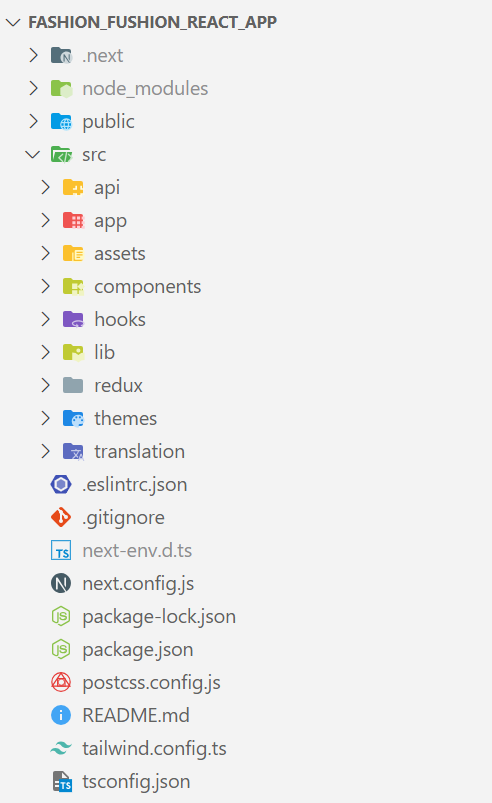
\includegraphics[width=0.6\linewidth]{Images/CodeFolder/WebFolder.png}
    \vspace{20pt}
    \caption{Cấu trúc thư mục ứng dụng web}
    \end{figure}

Tổng quan cấu trúc thư mục chính:
\begin{itemize}
    \item Thư mục api: Giao tiếp giữa Frontend và Backend thông qua api
    \item Thư mục app: Chứa các trang giao diện, layout chính của hệ thống 
    \item Thư mục assets: Chứa các hình ảnh, font chữ, css style sử dụng trong hệ thống
    \item Thư mục components: Chứa các thành phần tái sử dụng của hệ thống
    \item Thư mục hooks: Chứa các custom hooks của React
    \item Thư mục redux: Quản lý các trạng thái toàn cục (global state) của hệ thống
    \item Thư mục themes: Chứa các chủ đề (themes) của hệ thống 
    \item Thư mục translation: Chứa các thư viện, file dịch để sử dụng đa ngôn ngữ cho hệ thống
    
\end{itemize}

\subsubsection{Ứng dụng di động}
\begin{figure}[H]
    \centering
    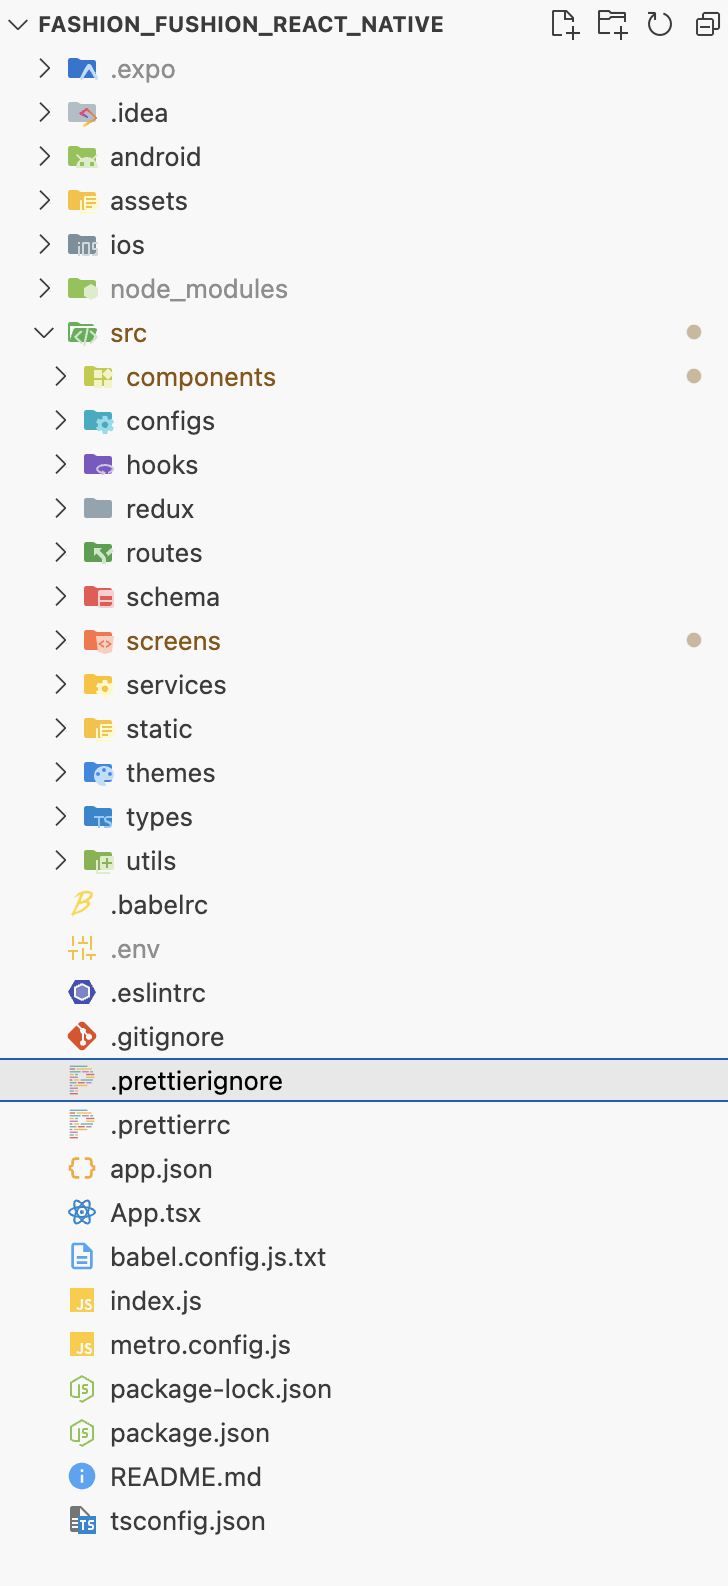
\includegraphics[width=0.4\linewidth]{Images/CodeFolder/mobileFolder.png}
    \vspace{20pt}
    \caption{Cấu trúc thư mục ứng dụng di động}
\end{figure}

Tổng quan cấu trúc thư mục chính:
\begin{itemize}
    \item Thư mục services: Giao tiếp giữa Frontend và Backend thông qua api
    \item Thư mục screens: Chứa tất cả cả màn hình của ứng dụng
    \item Thư mục static: Chứa các hình ảnh, logo và các icon sử dụng
    \item Thư mục components: Chứa các thành phần tái sử dụng của hệ thống
    \item Thư mục redux: Quản lý các trạng thái toàn cục (global state) của hệ thống
    \item Thư mục themes: Chứa các chủ đề (themes) của hệ thống 
    \item Thư mục route: Quản lý điều hướng giữa các màn hình ứng dụng
    \item Thư mục types: dùng để định nghĩa kiểu dữ liệu
    \item Thư mục android và ios: Chứa mã code native
    \item Thư mục util: Chứa các hàm công cụ xử lý
    \item Thư mục config: Chứa các constant và quản lý lỗi
    \item Thư mục hooks: Chứa các hook tự định nghĩa
    \item Thư mục schema: Chứa các cấu trúc dữ liệu và xử lý lỗi trong các Form
\end{itemize}
\subsubsection{Backend}
\begin{figure}[H]
    \centering
    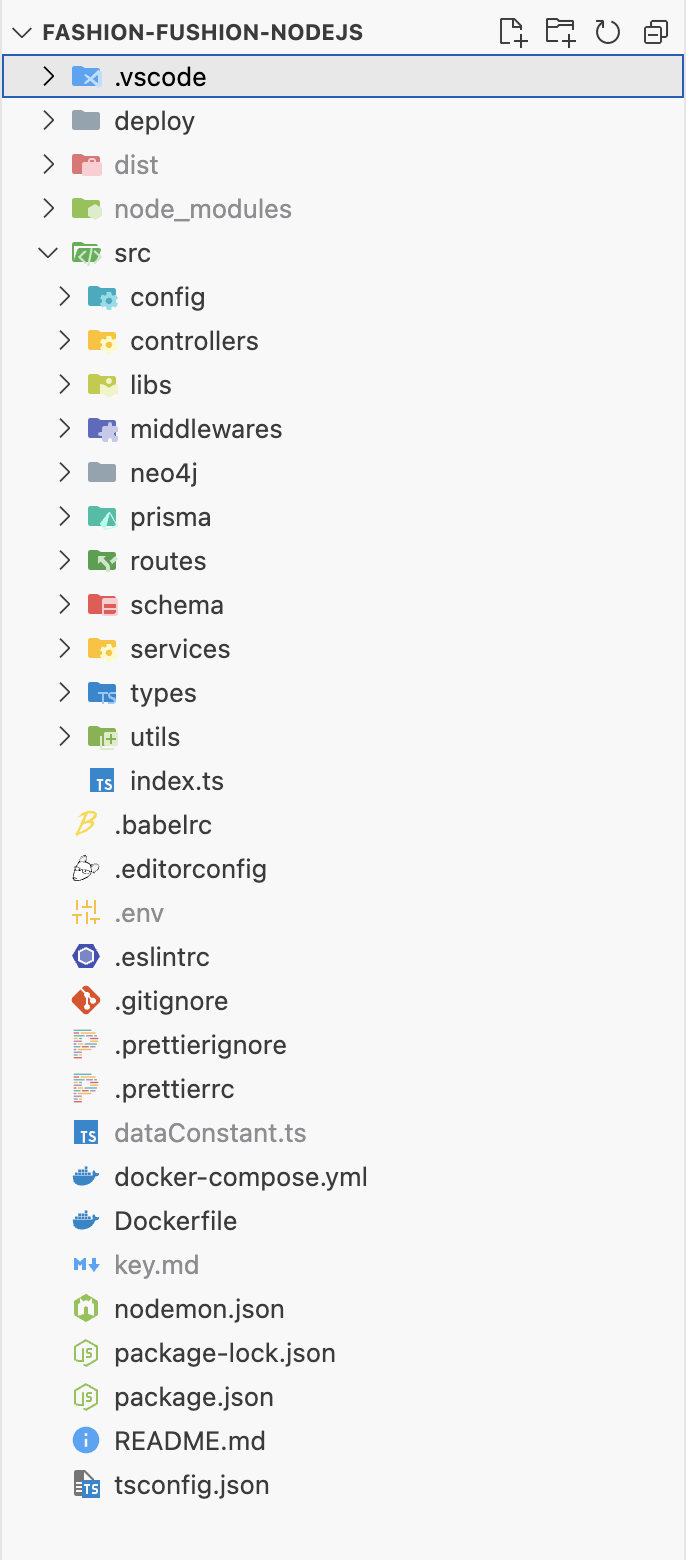
\includegraphics[width=0.4\linewidth]{Images/CodeFolder/backendFolder.png}
    \vspace{20pt}
    \caption{Cấu trúc thư mục Web service}
\end{figure}

Tổng quan cấu trúc thư mục chính:
\begin{itemize}
    \item Thư mục config: Chứa các constant và quản lý lỗi
    \item Thư mục controllers: Chịu trách nhiệm nhận yêu cầu từ client, thực hiện các xử lý cần thiết, và sau đó trả về phản hồi tương ứng
    \item Thư mục libs: Chứa các cài đặt về các thư viện được sử dụng như cổng thanh toán
    \item Thư mục middlewares: Thực hiện các quyền xác thực và xử lý dữ liệu
    \item Thư mục neo4j: Chứa các cài đặt về cơ sở dữ liệu Neo4j
    \item Thư mục prisma: Chứa các cài đặt ORM về cơ sở dữ liệu PosgreSQL
    \item Thư mục routes: Chứa các định nghĩa tuyến đường cho API
    \item Thư mục schema: Chứa các cấu trúc dữ liệu và xử lý lỗi trong các request
    \item Thư mục services: Chứa các thành phần xử lý nghiệp vụ
    \item Thư mục types: dùng để định nghĩa kiểu dữ liệu
    \item Thư mục util: Chứa các hàm công cụ xử lý
\end{itemize}
\subsection{Các API chính}
\begin{table}[H]
\centering
\begin{tabular}{|p{1.5cm}|p{6.5cm}|p{7cm}|}
\hline
Method & URL & Description \\
\hline
POST & /api/order/create & Tạo mới một order  \\
\hline
GET & /api/order/admin & Admin lấy danh sách các order  \\
\hline
GET & /api/order/detail & Lấy thông tin chi tiết của order  \\
\hline
POST & /api/product & Tạo mới một sản phẩm  \\
\hline
POST & /api/product/variant & Tạo mới một variant \\
\hline
POST & /api/product/filter & Filter thông tin và lấy các variant hợp lệ \\
\hline
PATCH & /api/product/variant/image & Thêm ảnh cho variant\\
\hline
GET & /api/product/detail & Lấy thông tin chi tiết của một sản phẩm\\
\hline
GET & /api/user/cart & Lấy các variant từ giỏ hàng\\
\hline
POST & /api/user/cart & Thêm mới một sản phẩm vào giỏ hàng\\
\hline
PATCH & /api/user/cart & Thay đổi số lượng variant trong giỏ hàng\\
\hline
GET & /api/user/wish & Lấy các sản phẩm từ danh sách yêu thích\\
\hline
POST & /api/user/wish & Thêm mới một sản phẩm vào danh sách yêu thích\\
\hline

GET & /api/user/viewed & Lấy các sản phẩm từ danh sách mà người dùng đã xem\\
\hline



\end{tabular}
\end{table}
\newpage

\begin{table}[H]
\centering
\begin{tabular}{|p{1.5cm}|p{6.5cm}|p{7cm}|}
\hline
Method & URL & Description \\
\hline
POST & /api/user/viewed & Thêm mới một sản phẩm vào danh sách mà người dùng đã xem\\
\hline
GET & /api/user/recommendbyuser & Lấy các sản phẩm được gợi ý cho người dùng\\
\hline
POST & /api/user/recommendbyotheruser & Lấy các sản phẩm được gợi ý từ người dùng khác\\
\hline
POST & /api/review & Tạo mới một review\\
\hline
PATCH & /api/review/is-disable & Staff cập nhật disable cho review\\
\hline
GET & /api/staff/over-view & Staff lấy các thông tin overview của trang dashboard\\
\hline
GET & /api/staff/revenue & Staff lấy các thông tin doanh thu theo từng ngày trong khoảng thời gian chỉ định\\
\hline
GET & /api/staff/best-selling & Staff lấy các thông tin các sản phẩm có số lượng mua cao nhất trong khoảng thời gian chỉ định\\
\hline
POST & /fastapi/upload & Chuyển ảnh của các sản phẩm thành các vector\\
\hline
POST & /fastapi/search\_base64 & Nhận ảnh của người dùng để tiến hành tìm kiếm ảnh tương đồng\\
\hline
POST & /api/voucher & Tạo mới một voucher\\
\hline

\end{tabular}
\caption{Bảng các API chính}
\end{table}

\subsection{Giao diện hệ thống}
\subsubsection{Giao diện web của quản trị viên}

\begin{itemize}
    \item \textbf{Trang điều khiển (Dashboard)}
\end{itemize}
 \begin{figure}[H]
        \centering
        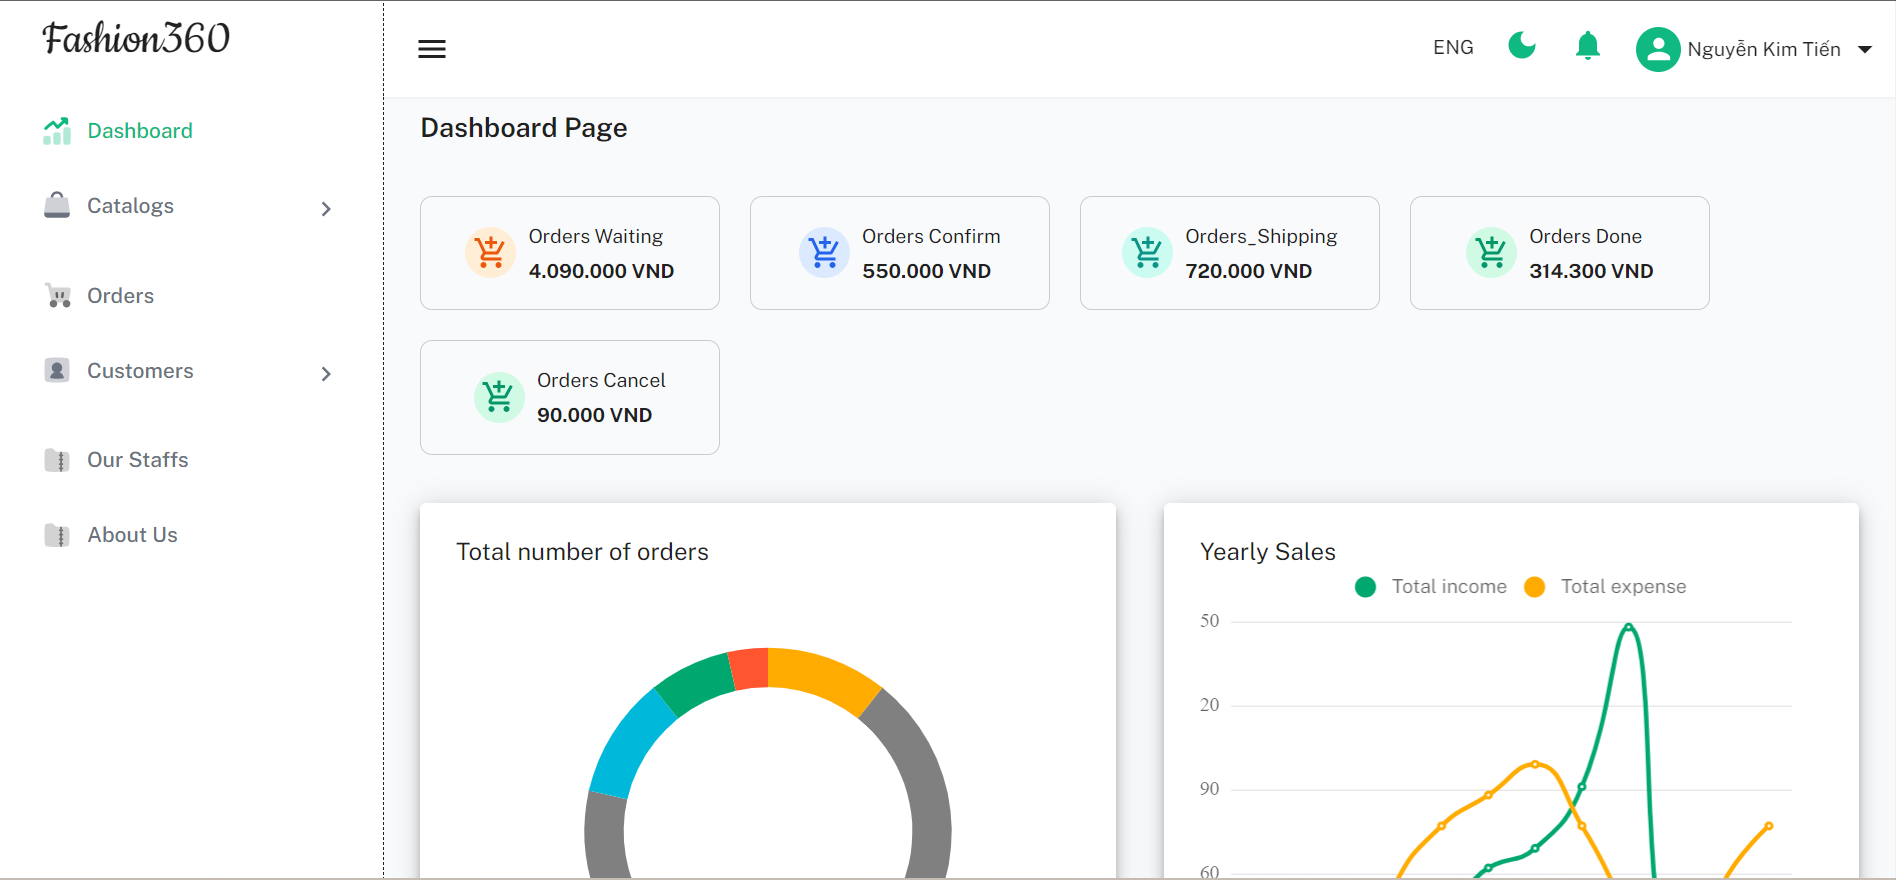
\includegraphics[width=14cm]{Images/Web/dashboard.png}
        \newline
        \caption{Một phần giao diện của trang điều khiển (Dashboard)}
\end{figure}
 \begin{figure}[H]
        \centering
        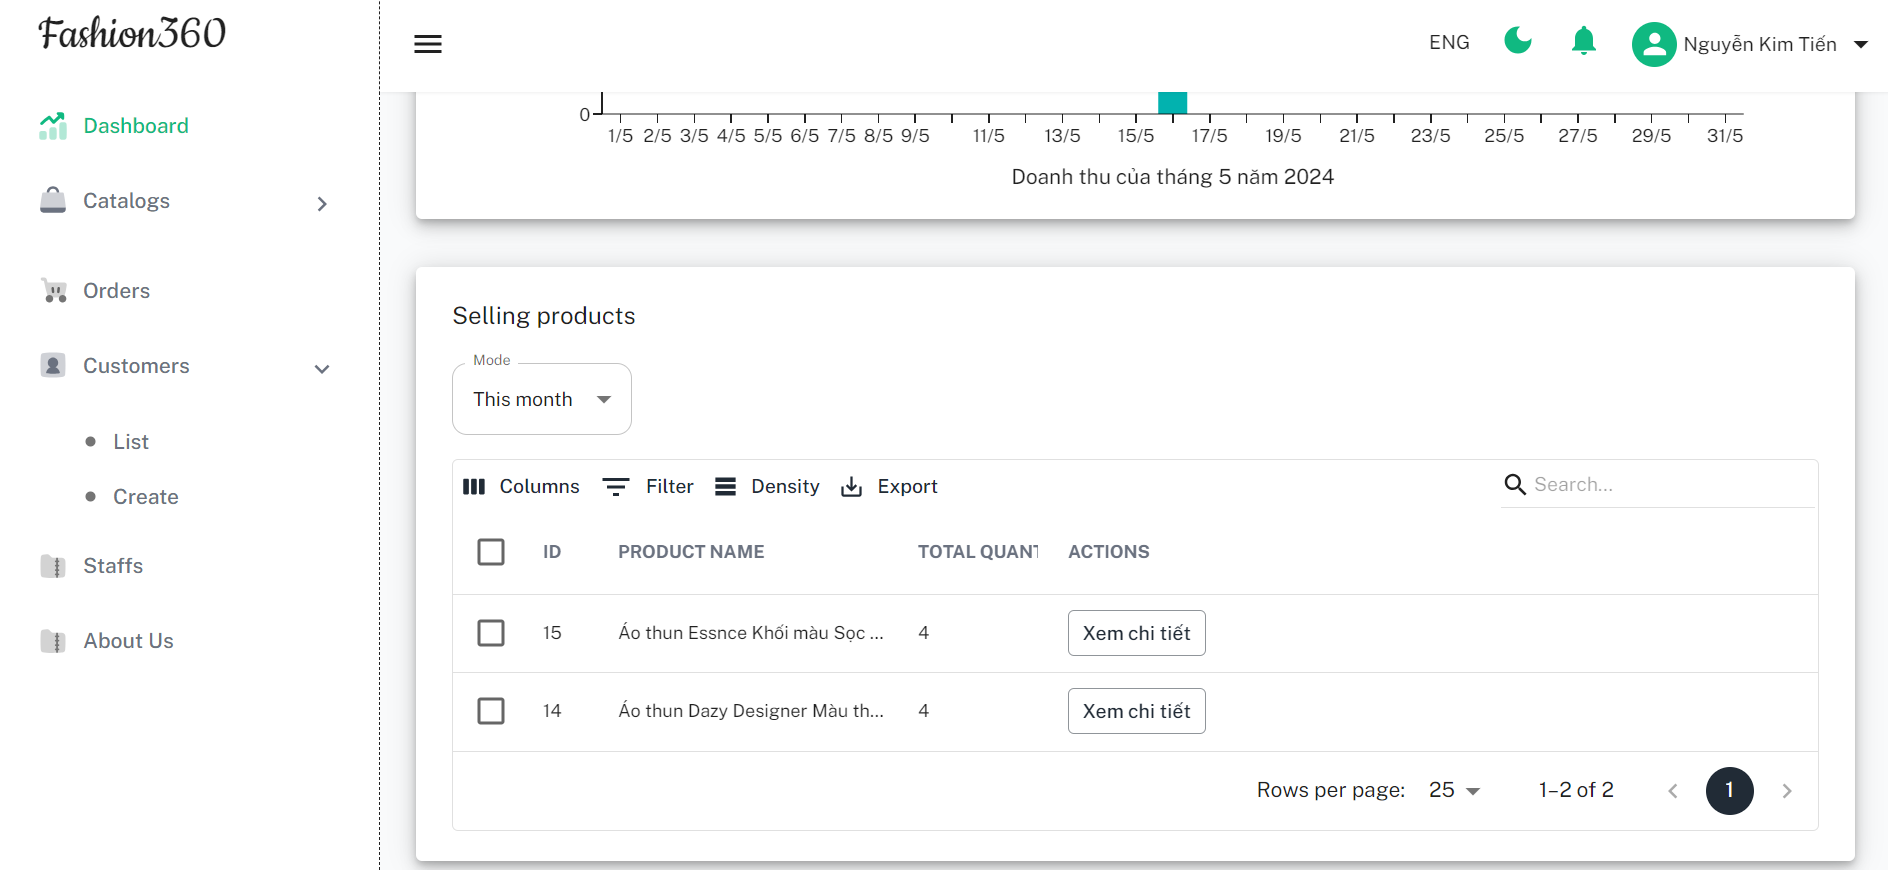
\includegraphics[width=14cm]{Images/Web/dashboard2.png}
        \newline
        \caption{Một phần giao diện của trang điều khiển (Dashboard)}
\end{figure}

\begin{itemize}
    \item \textbf{Trang thể loại (Category)}
\end{itemize}
 \begin{figure}[H]
        \centering
        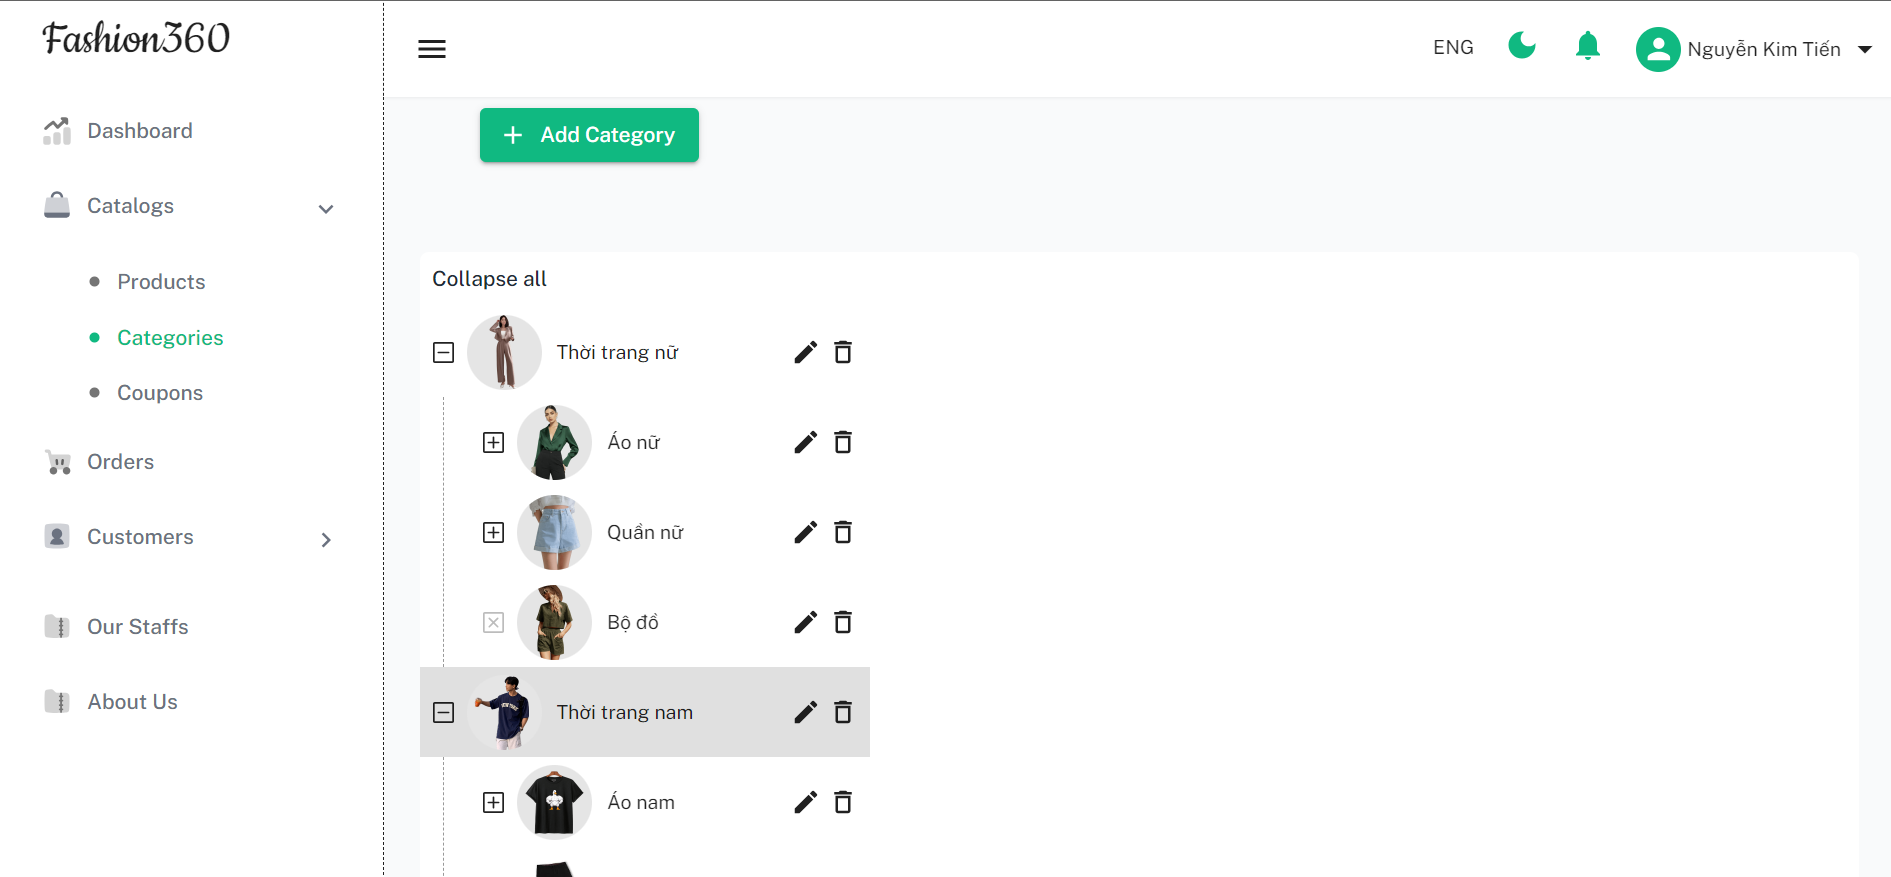
\includegraphics[width=14cm]{Images/Web/category.png}
        \newline
        \caption{Giao diện hiển thị danh sách thể loại}
\end{figure}
\begin{figure}[H]
        \centering
        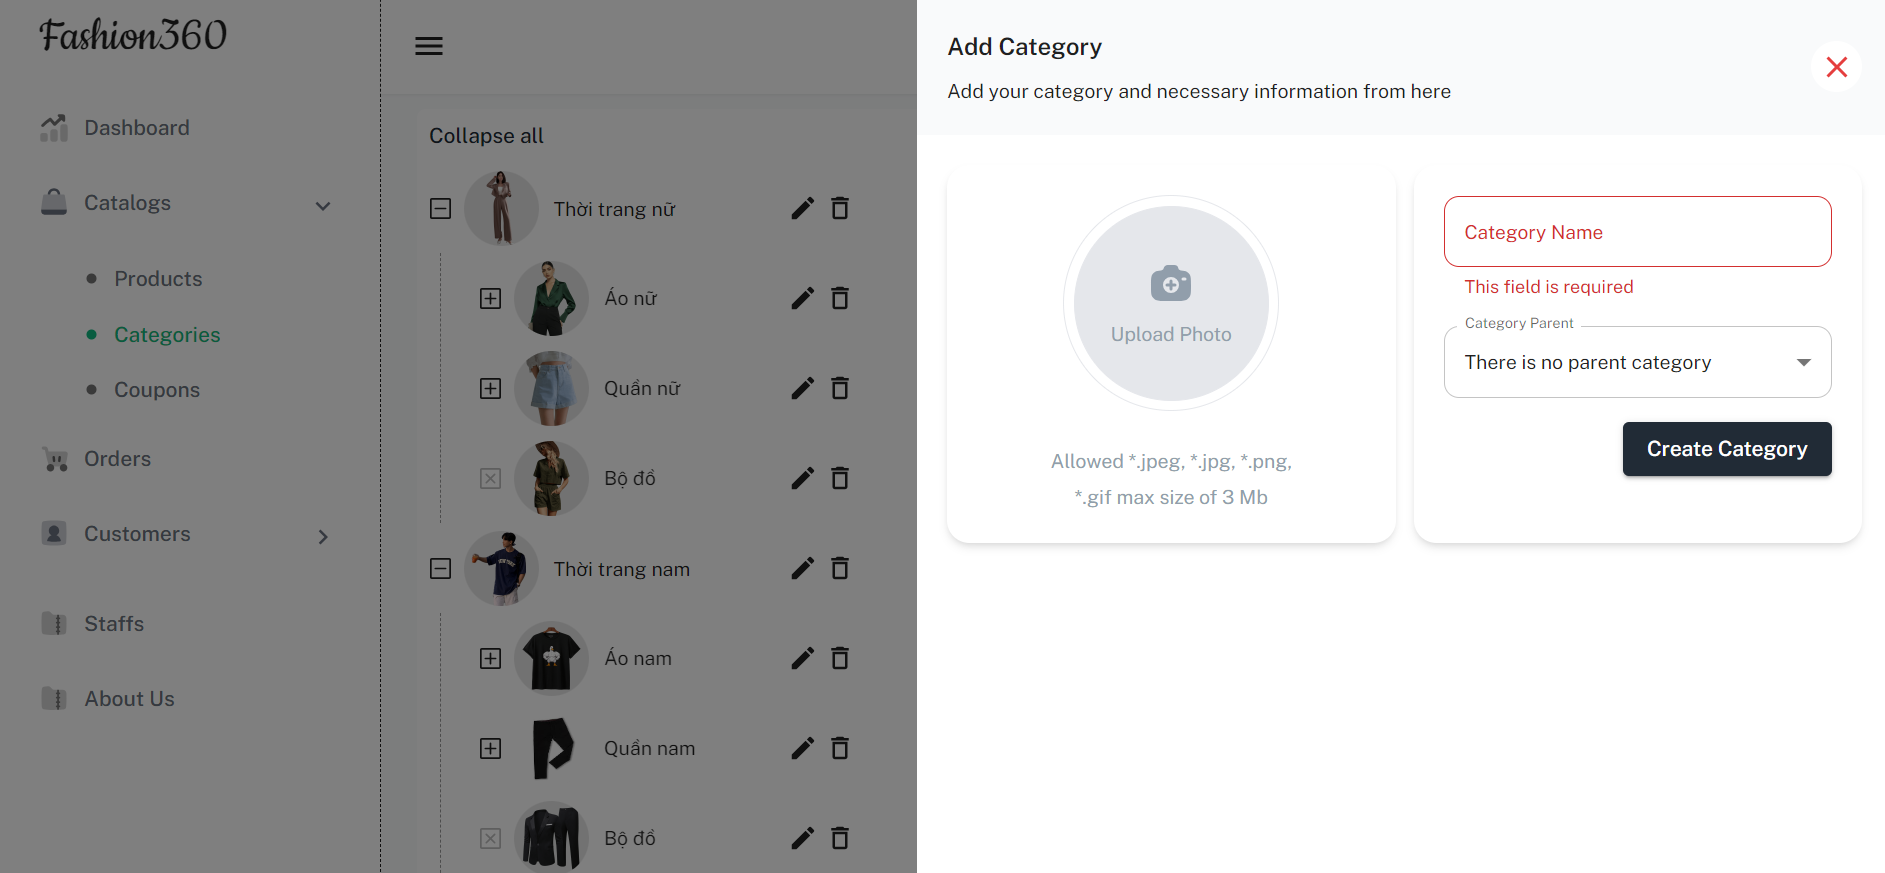
\includegraphics[width=14cm]{Images/Web/addCategory.png}
        \newline
        \caption{Giao diện của trang tạo mới thể loại}
\end{figure}
\begin{figure}[H]
        \centering
        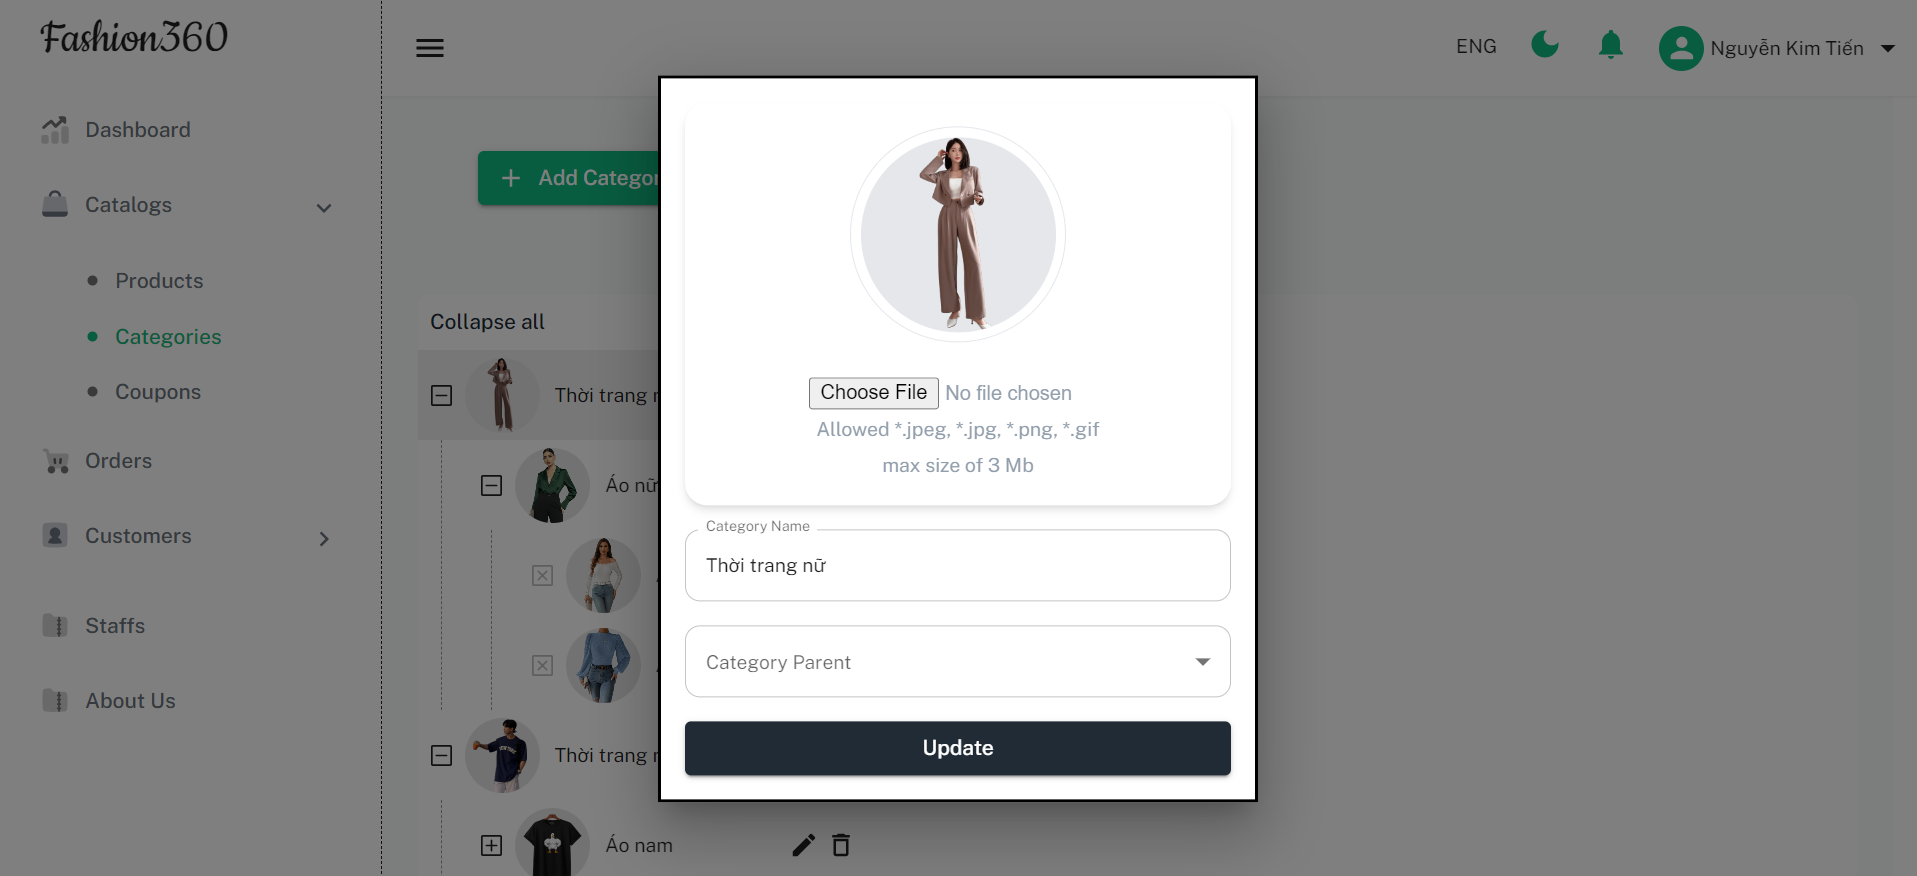
\includegraphics[width=14cm]{Images/Web/updateCategory.png}
        \newline
        \caption{Giao diện của trang cập nhật thể loại}
\end{figure}

\begin{itemize}
    \item \textbf{Trang sản phẩm (Product)}
\end{itemize}
 \begin{figure}[H]
        \centering
        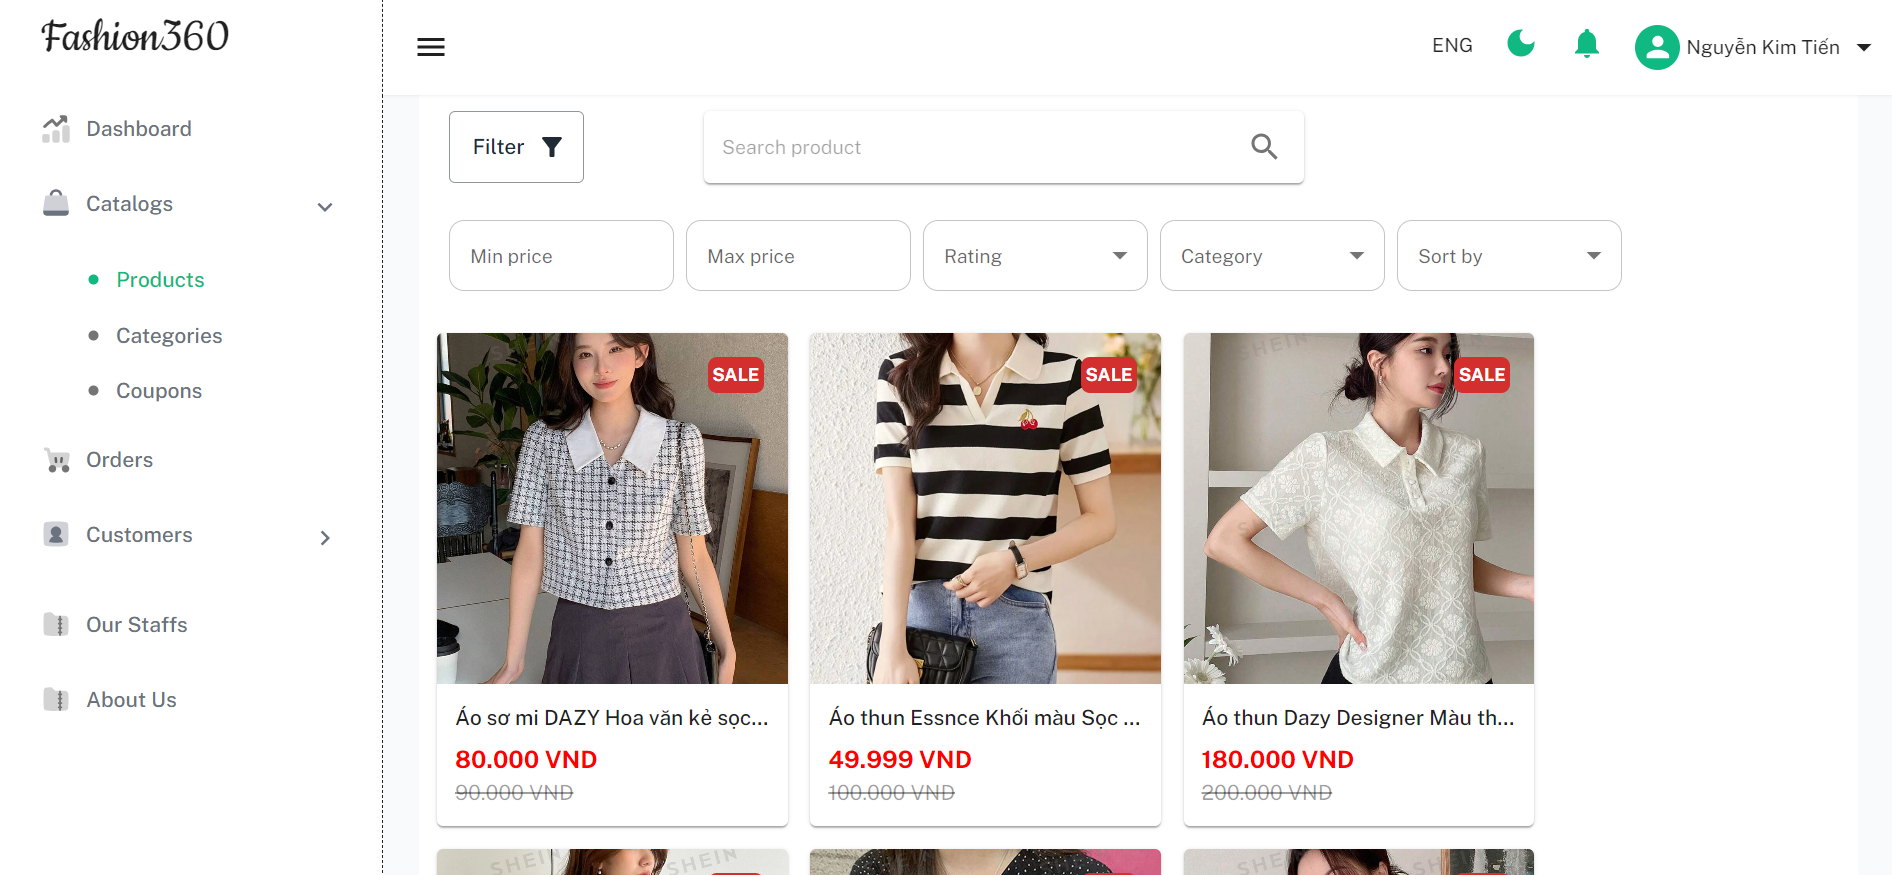
\includegraphics[width=14cm]{Images/Web/productList.png}
        \newline
        \caption{Một phần giao diện hiển thị danh sách sản phẩm}
\end{figure}
 \begin{figure}[H]
        \centering
        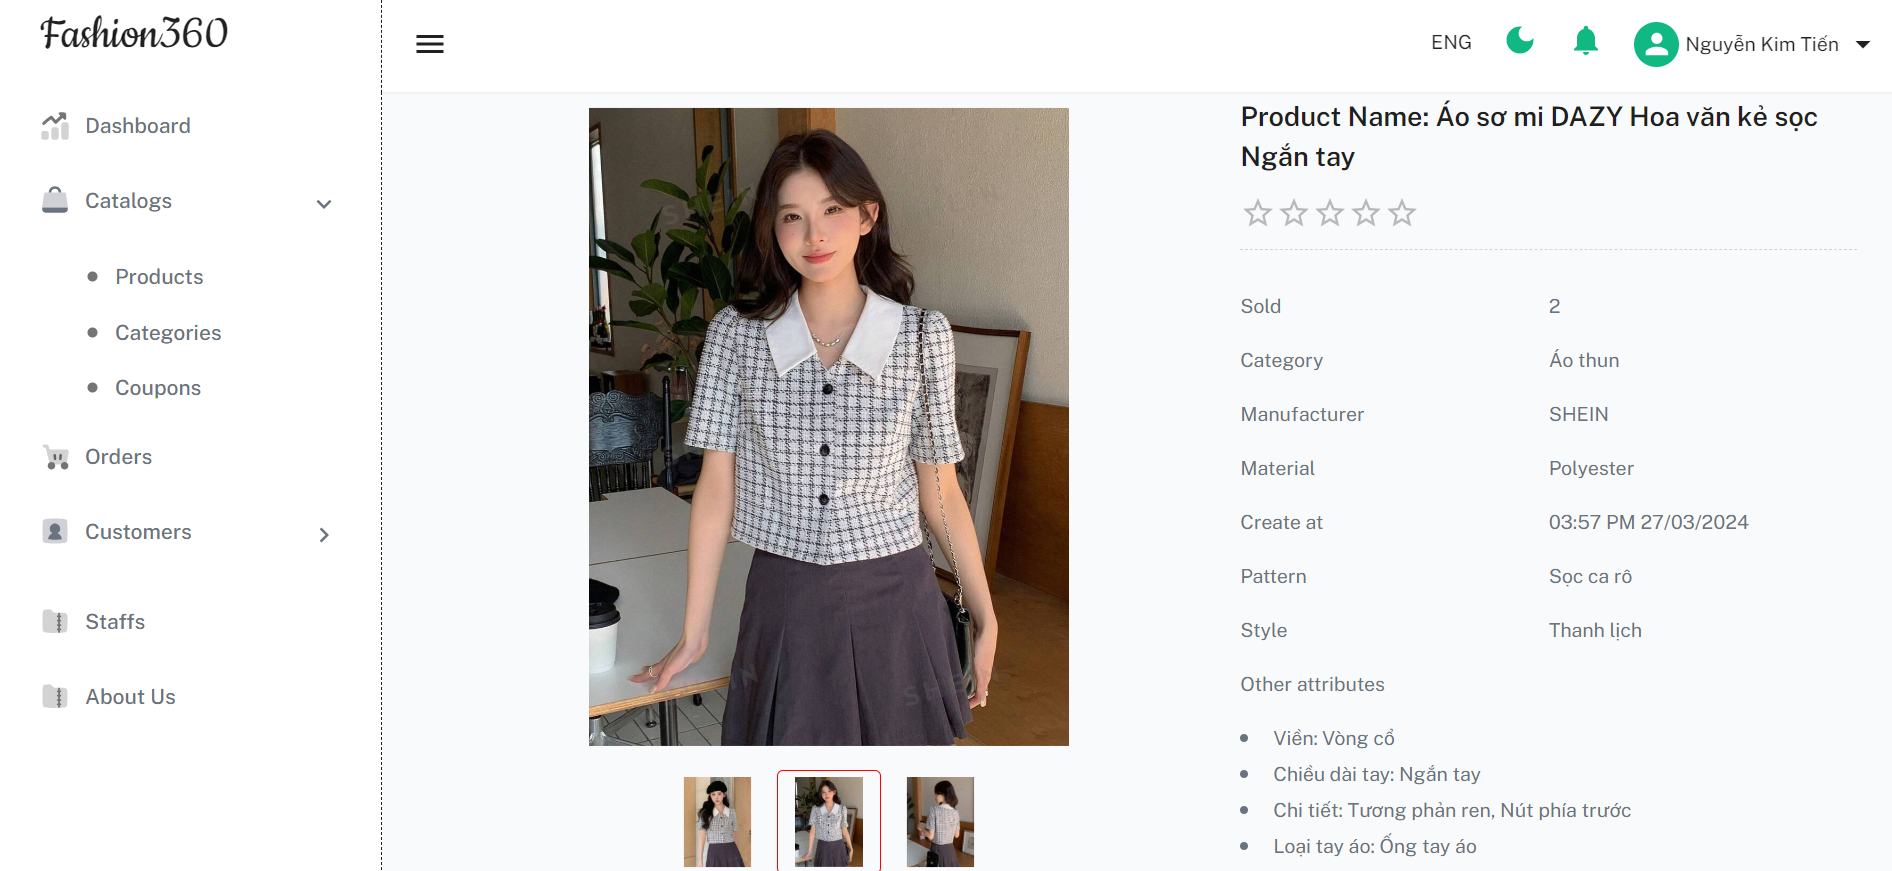
\includegraphics[width=14cm]{Images/Web/productDetail.png}
        \newline
        \caption{Một phần giao diện hiển thị thông tin chi tiết sản phẩm}
\end{figure}
\begin{figure}[H]
        \centering
        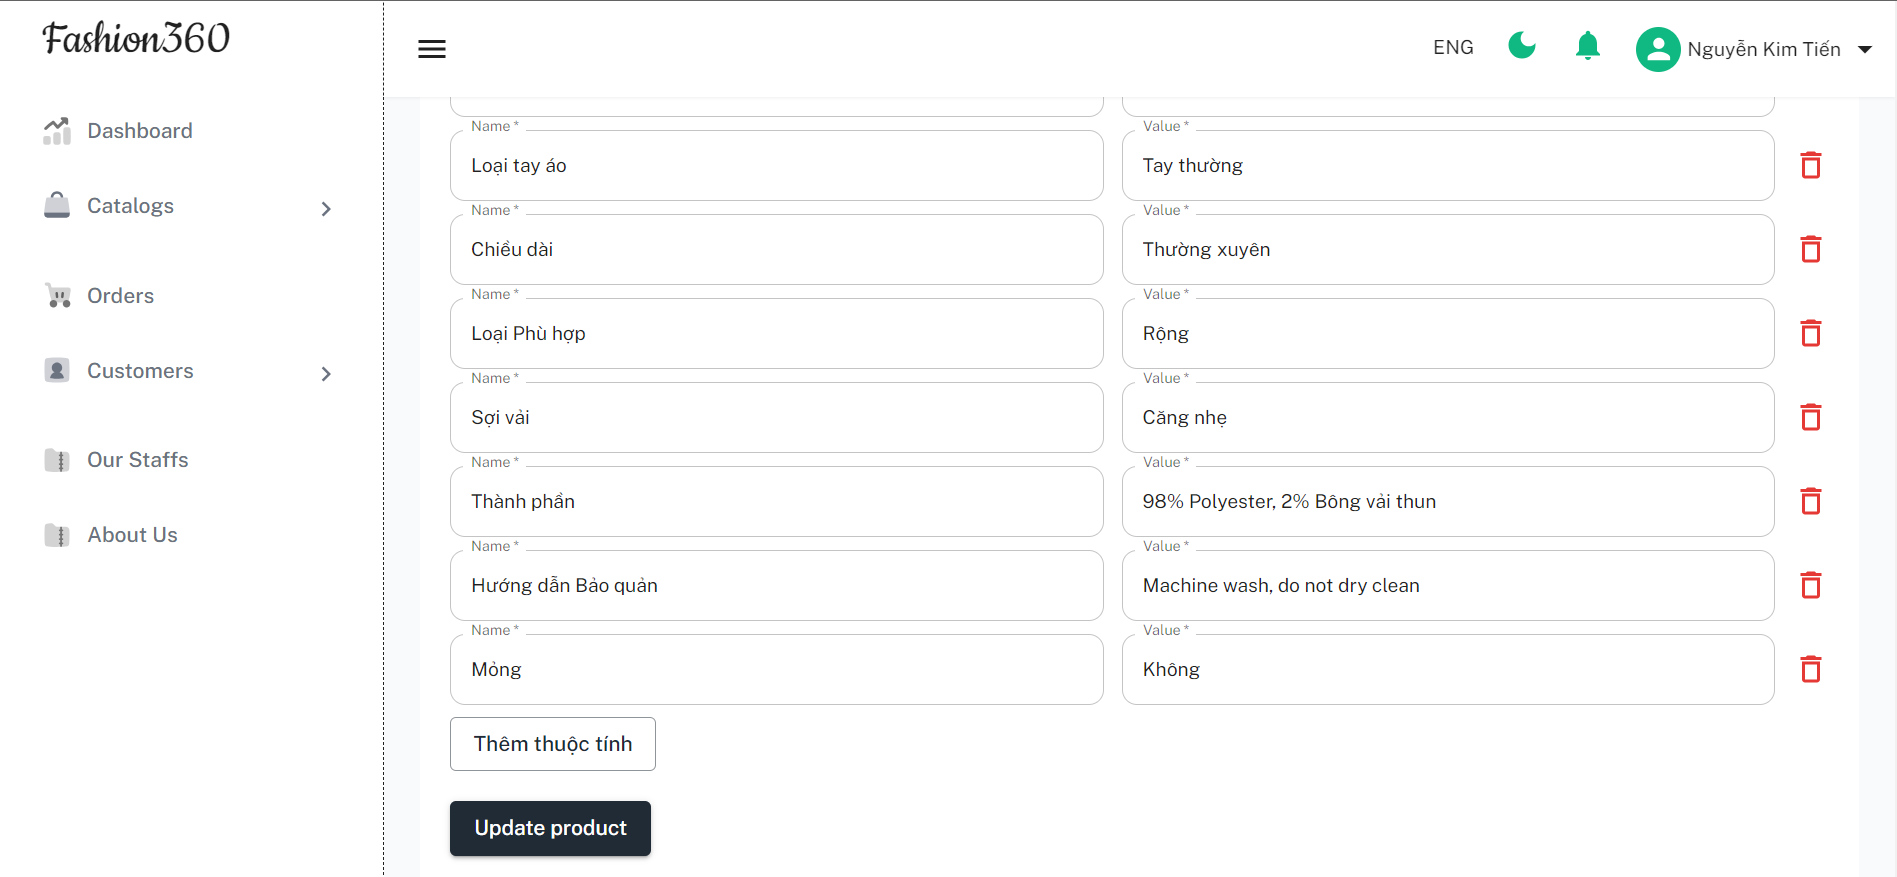
\includegraphics[width=14cm]{Images/Web/updateProduct.png}
        \newline
        \caption{Một phần giao diện của trang cập nhật sản phẩm}
\end{figure}

\begin{itemize}
    \item \textbf{Trang Variant}
\end{itemize}
 \begin{figure}[H]
        \centering
        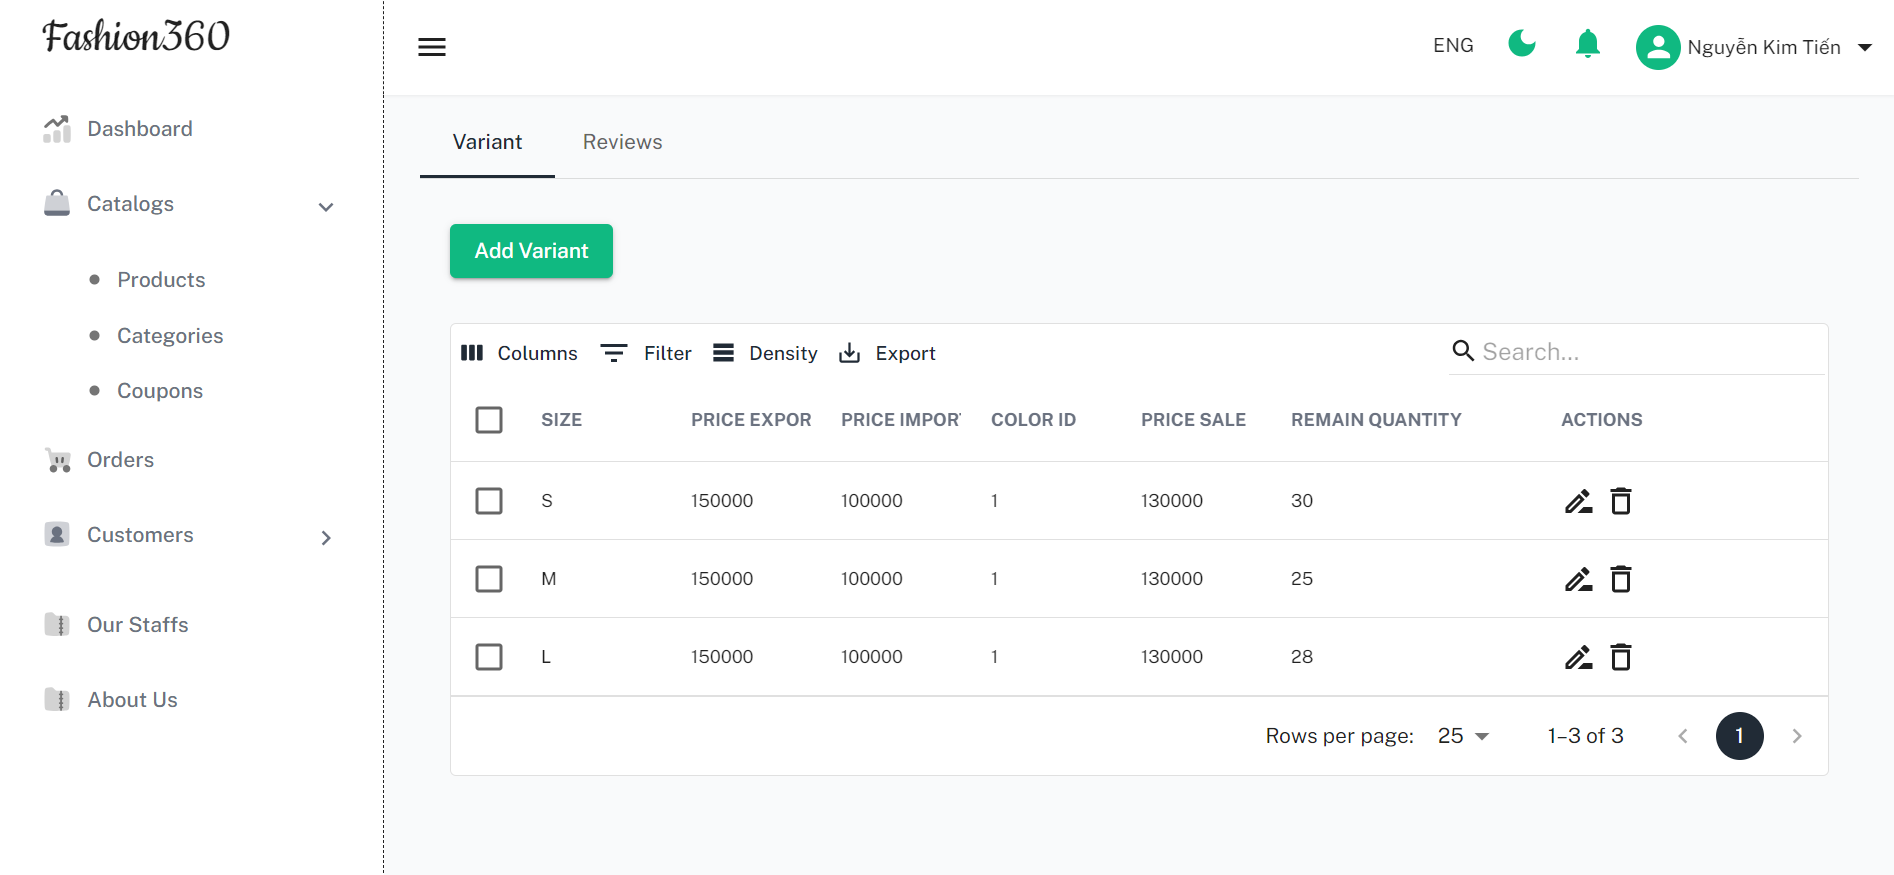
\includegraphics[width=14cm]{Images/Web/variant.png}
        \newline
        \caption{Một phần giao diện hiển thị danh sách Variant}
\end{figure}
 \begin{figure}[H]
        \centering
        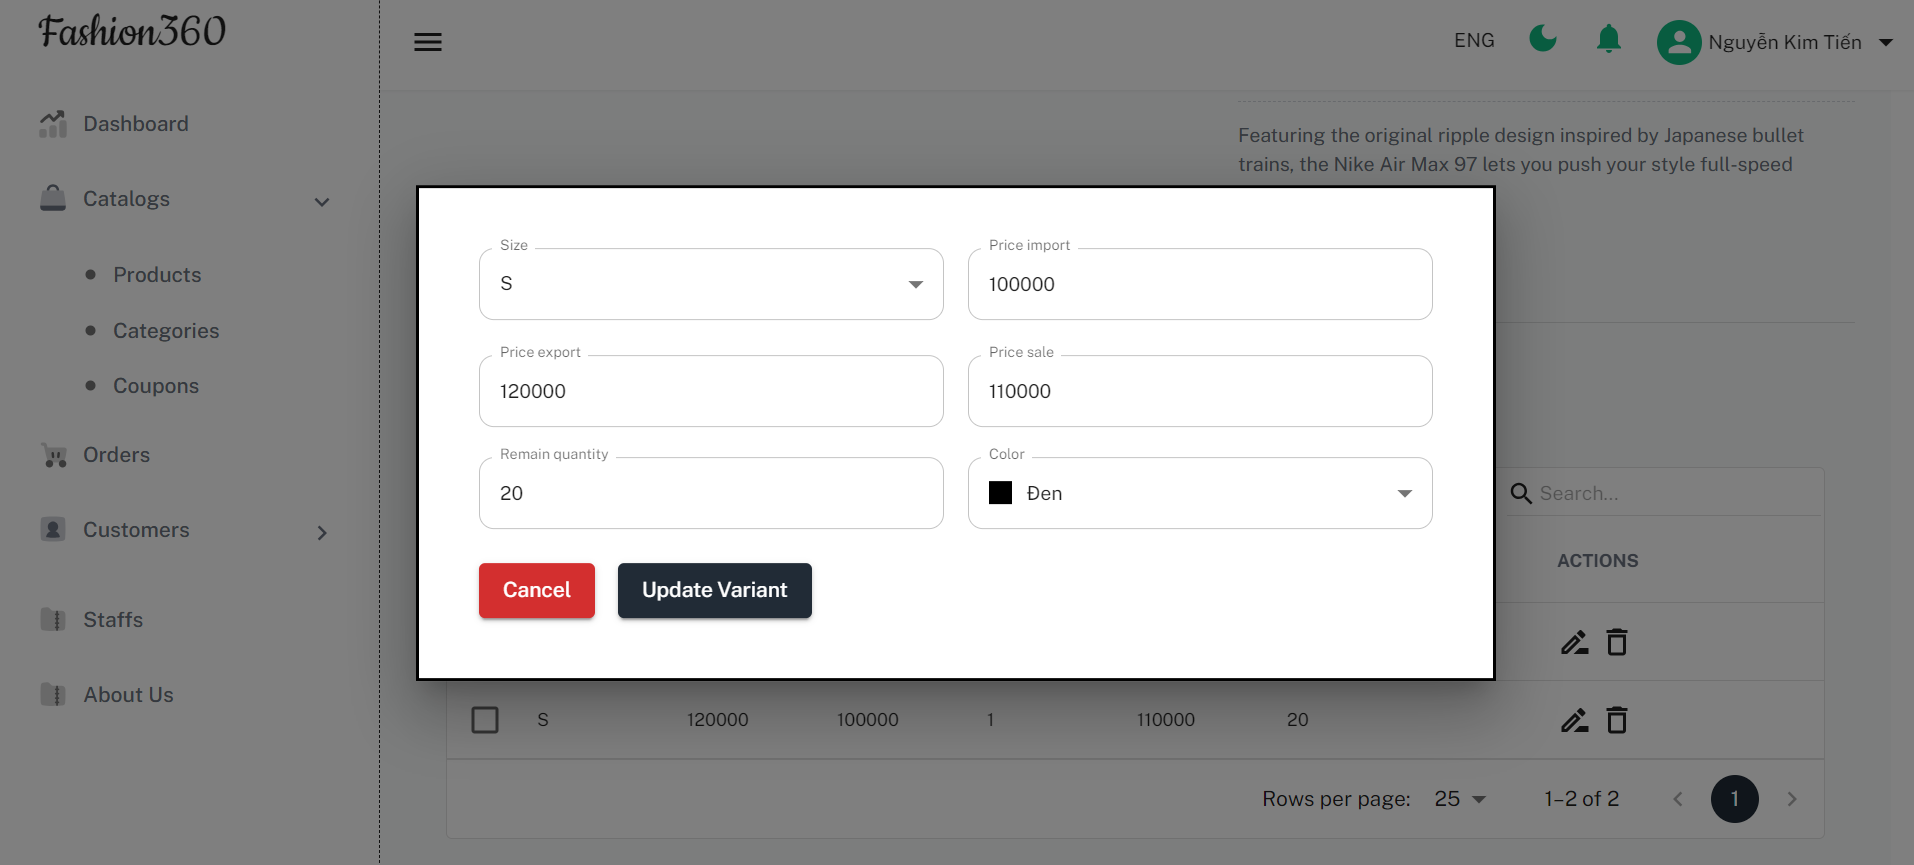
\includegraphics[width=14cm]{Images/Web/updateVariant.png}
        \newline
        \caption{Giao diện của trang cập nhật Variant}
\end{figure}

\begin{itemize}
    \item \textbf{Trang mã giảm giá (Coupons)}
\end{itemize}
 \begin{figure}[H]
        \centering
        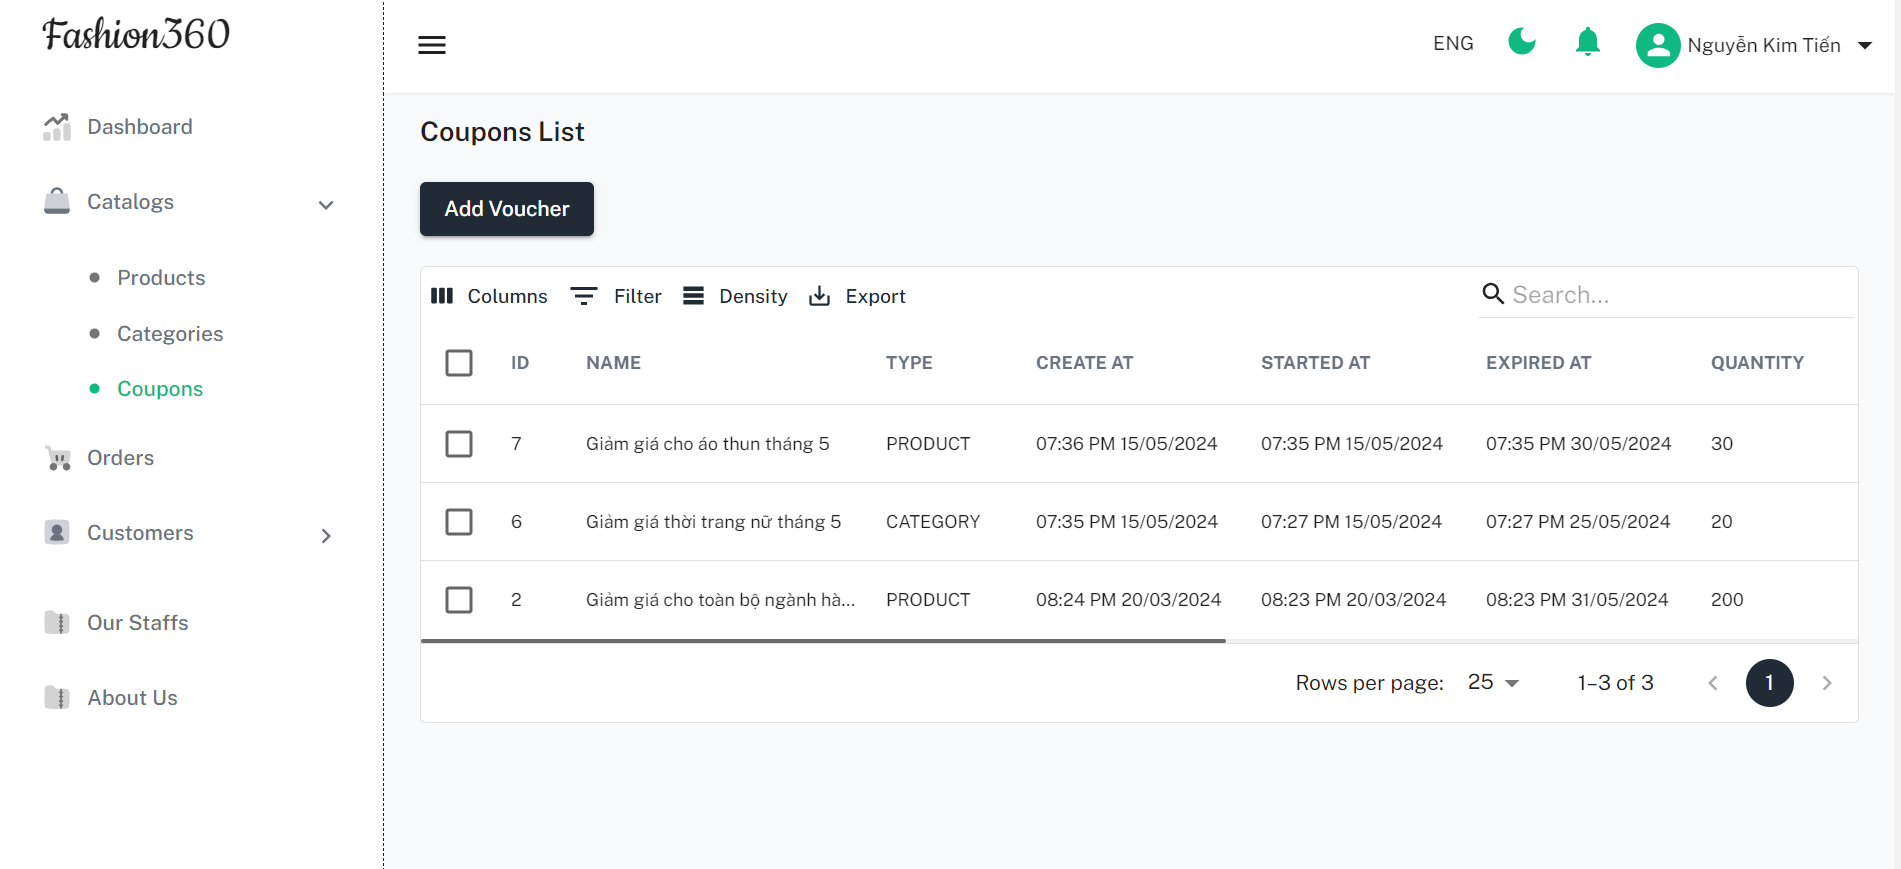
\includegraphics[width=14cm]{Images/Web/voucher.png}
        \newline
        \caption{Giao diện hiển thị danh sách mã giảm giá}
\end{figure}

\begin{figure}[H]
        \centering
        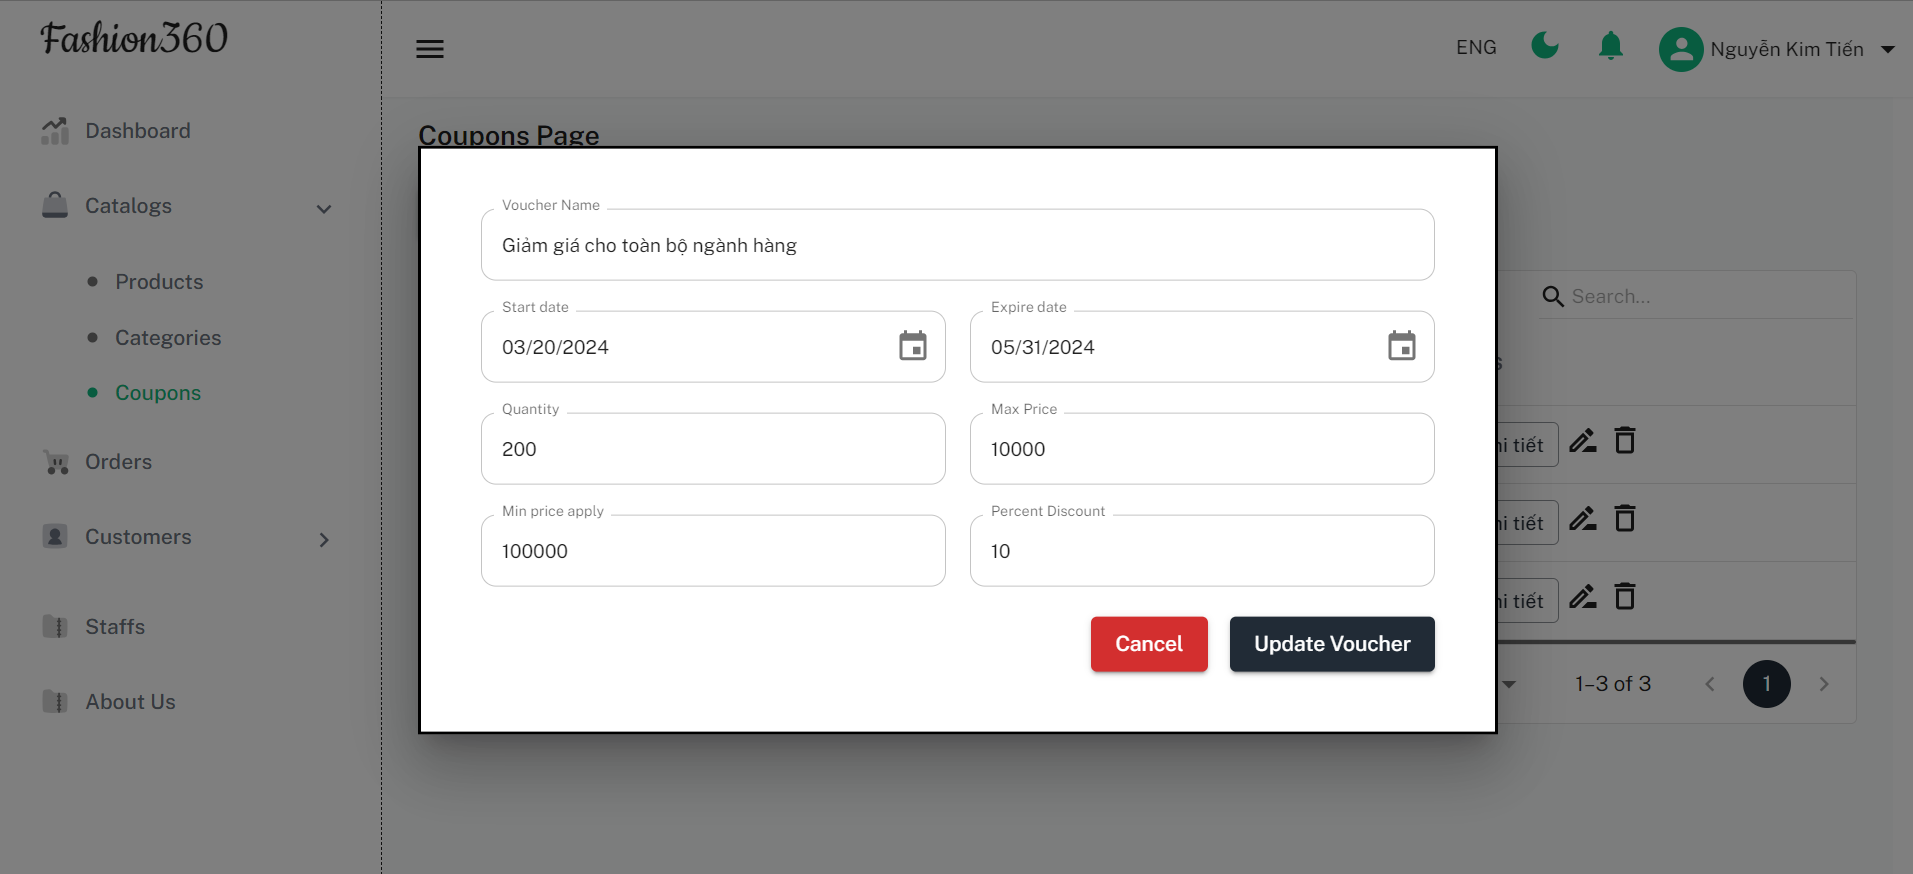
\includegraphics[width=14cm]{Images/Web/updateVoucher.png}
        \newline
        \caption{Giao diện của trang cập nhật mã giảm giá}
\end{figure}
 \begin{figure}[H]
        \centering
        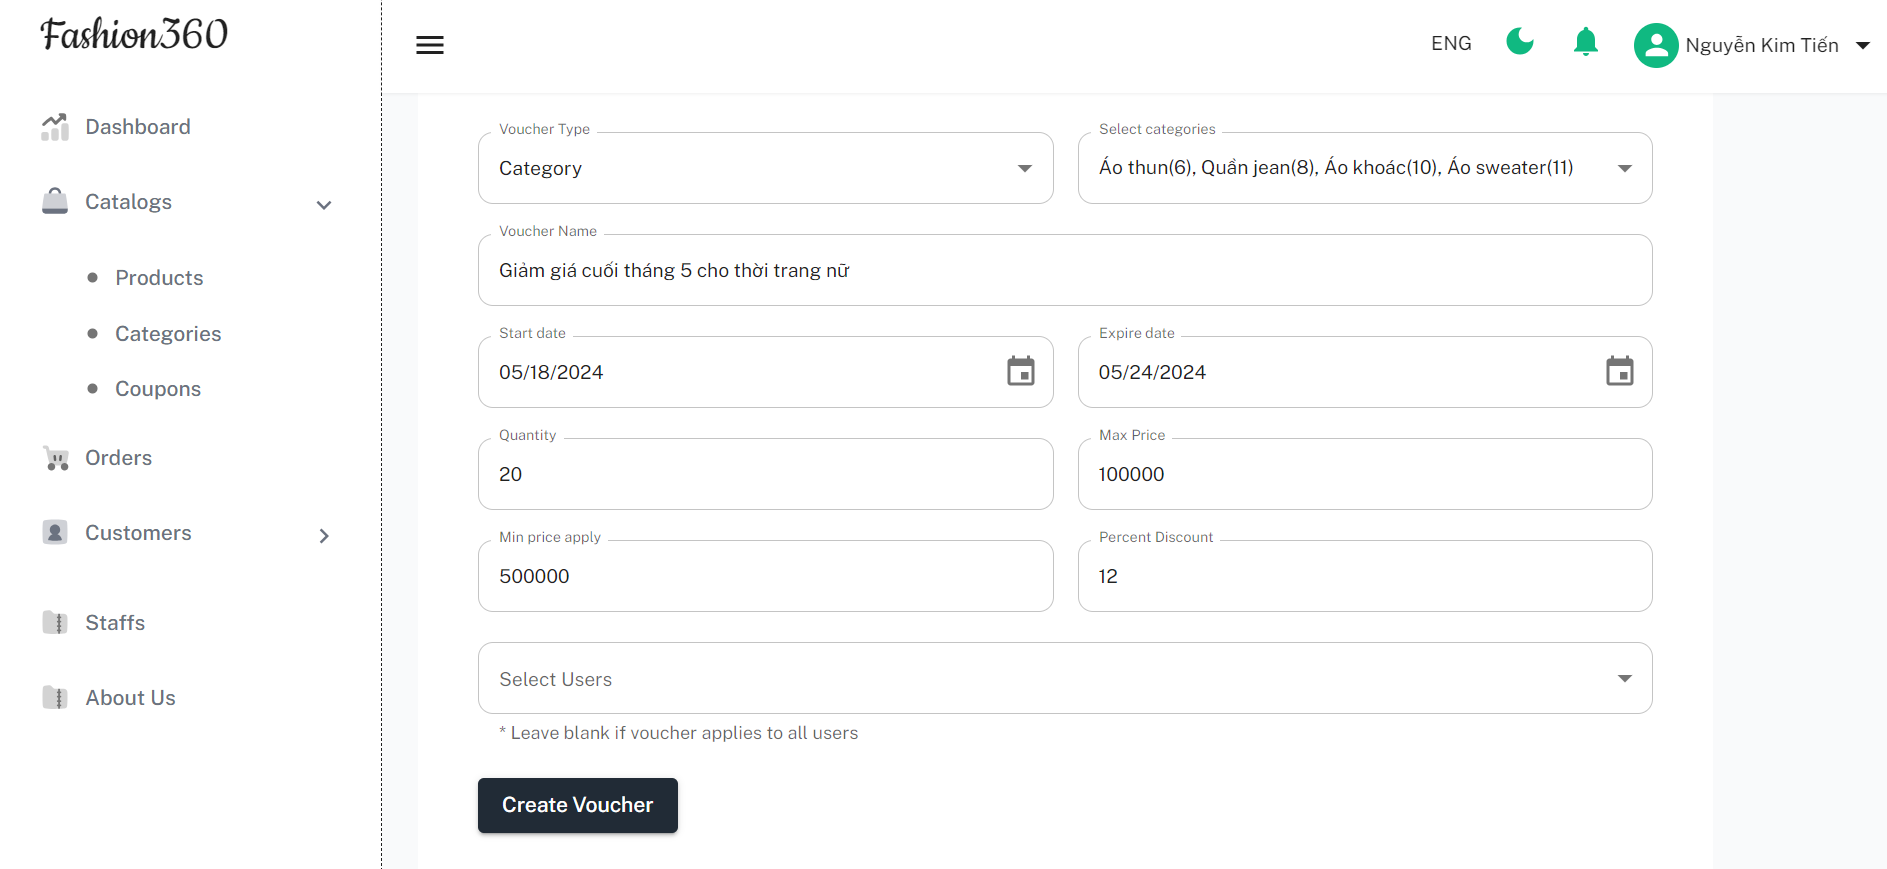
\includegraphics[width=14cm]{Images/Web/addVoucher.png}
        \newline
        \caption{Một phần giao diện của trang tạo mới mã giảm giá}
\end{figure}
 \begin{figure}[H]
        \centering
        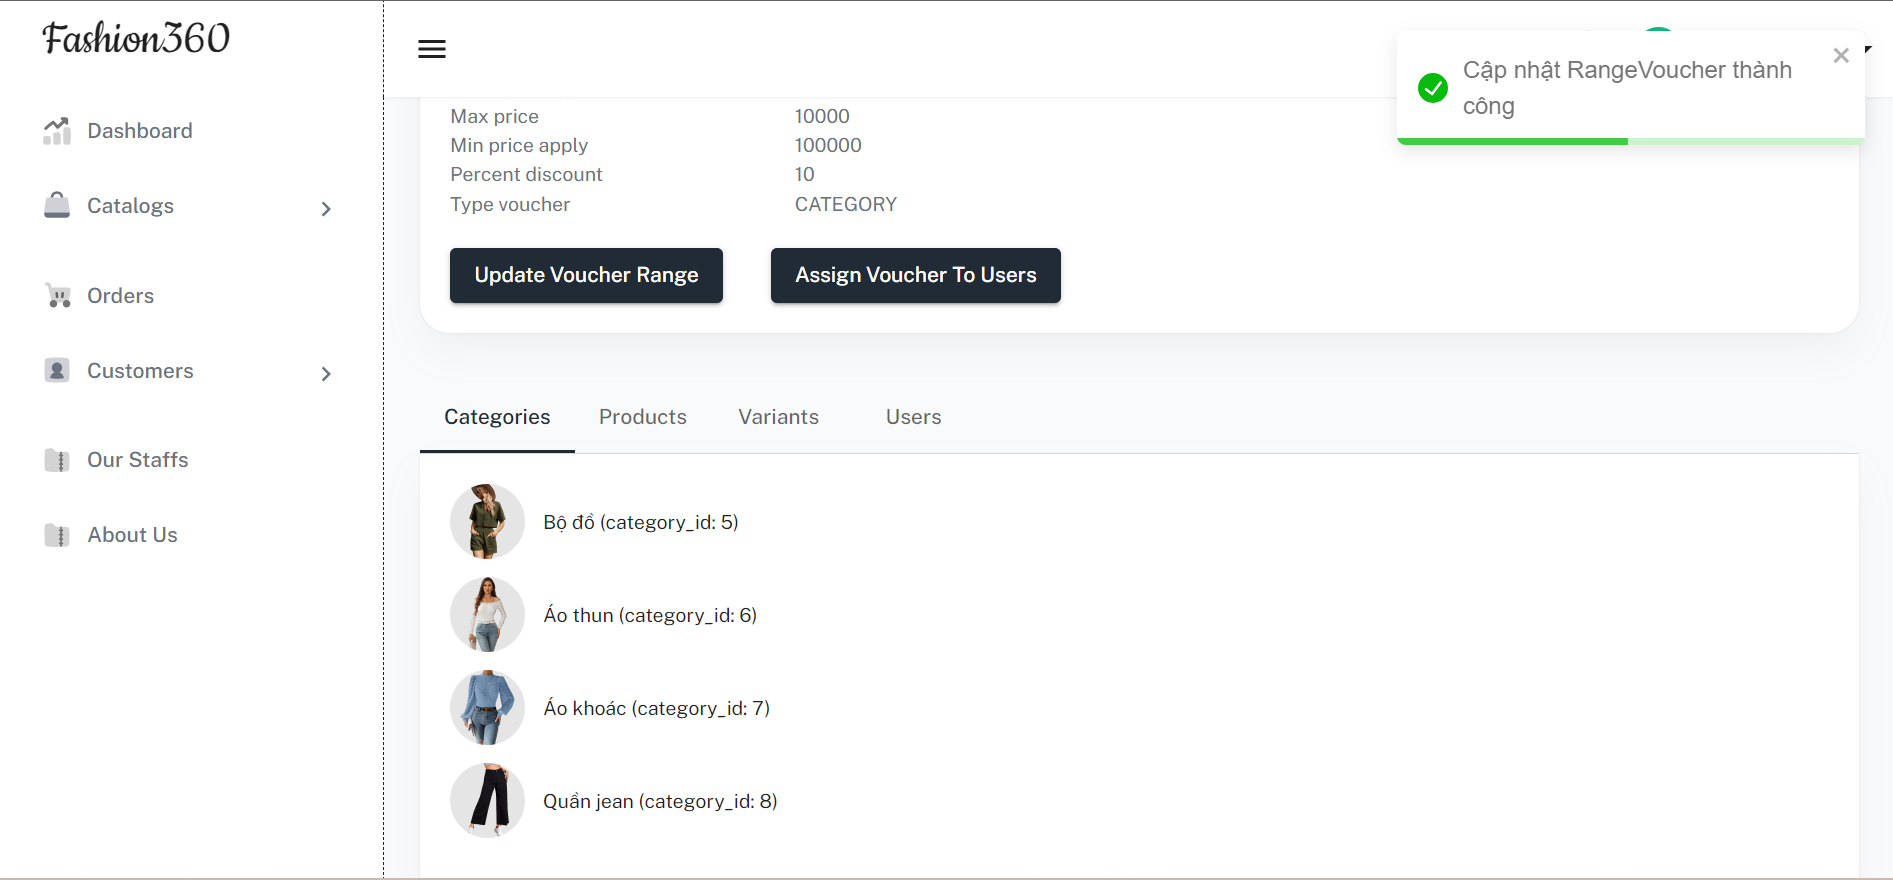
\includegraphics[width=14cm]{Images/Web/updateVoucherCategory.png}
        \newline
        \caption{Một phần giao diện của trang gán mã giảm giá cho thể loại}
\end{figure}
 \begin{figure}[H]
        \centering
        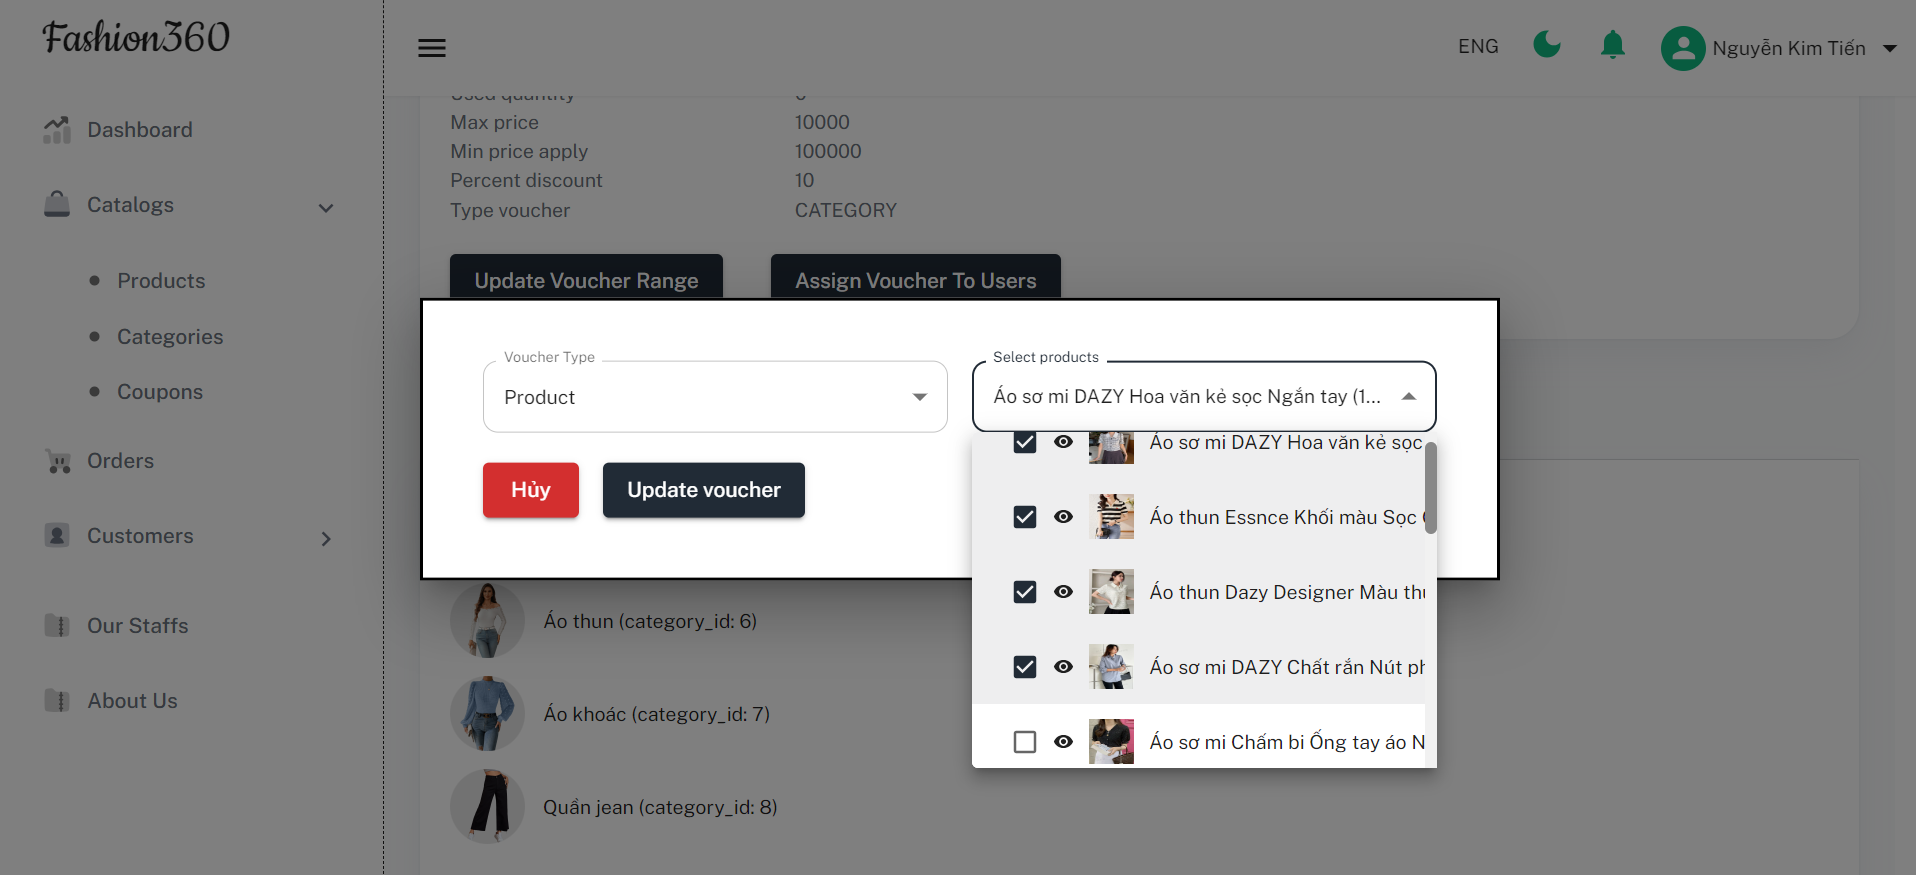
\includegraphics[width=14cm]{Images/Web/updateVoucherProduct.png}
        \newline
        \caption{Một phần giao diện của trang gán mã giảm giá cho sản phẩm}
\end{figure}
\begin{figure}[H]
        \centering
        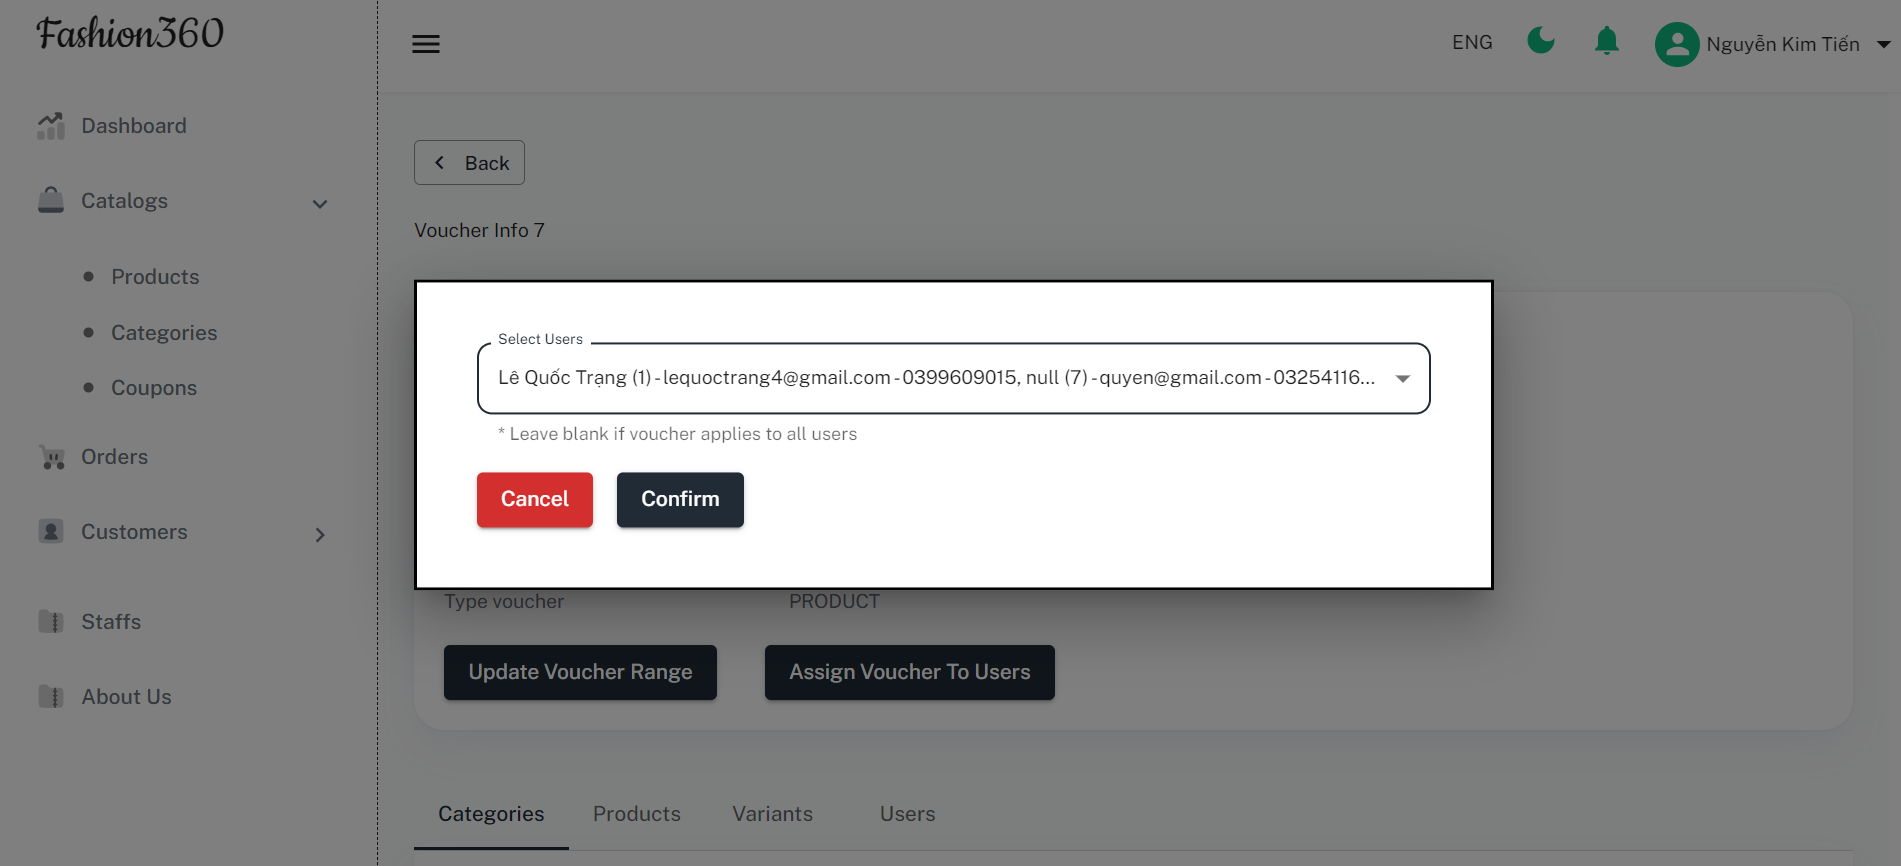
\includegraphics[width=14cm]{Images/Web/updateVoucherUser.png}
        \newline
        \caption{Một phần giao diện của trang gán mã giảm giá cho người dùng}
\end{figure}

\begin{itemize}
    \item \textbf{Trang Đơn hàng (Order)}
\end{itemize}
\begin{figure}[H]
        \centering
        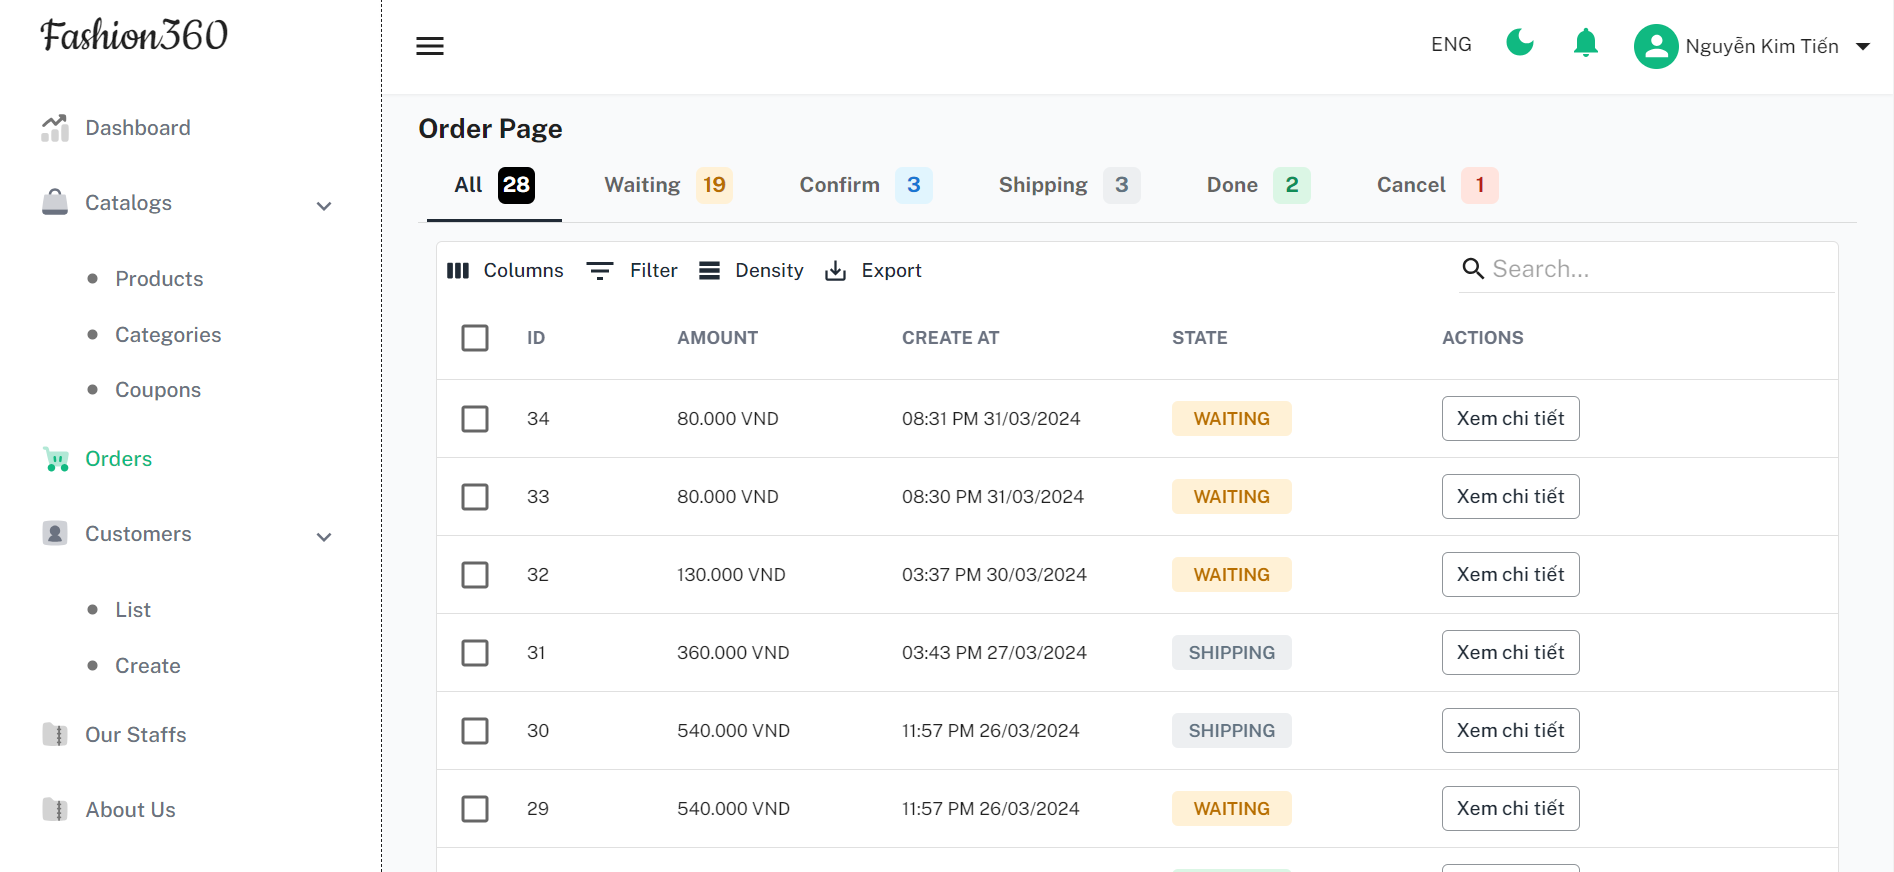
\includegraphics[width=14cm]{Images/Web/order.png}
        \newline
        \caption{Một phần giao diện hiển thị danh sách đơn hàng}
\end{figure}
\begin{figure}[H]
        \centering
        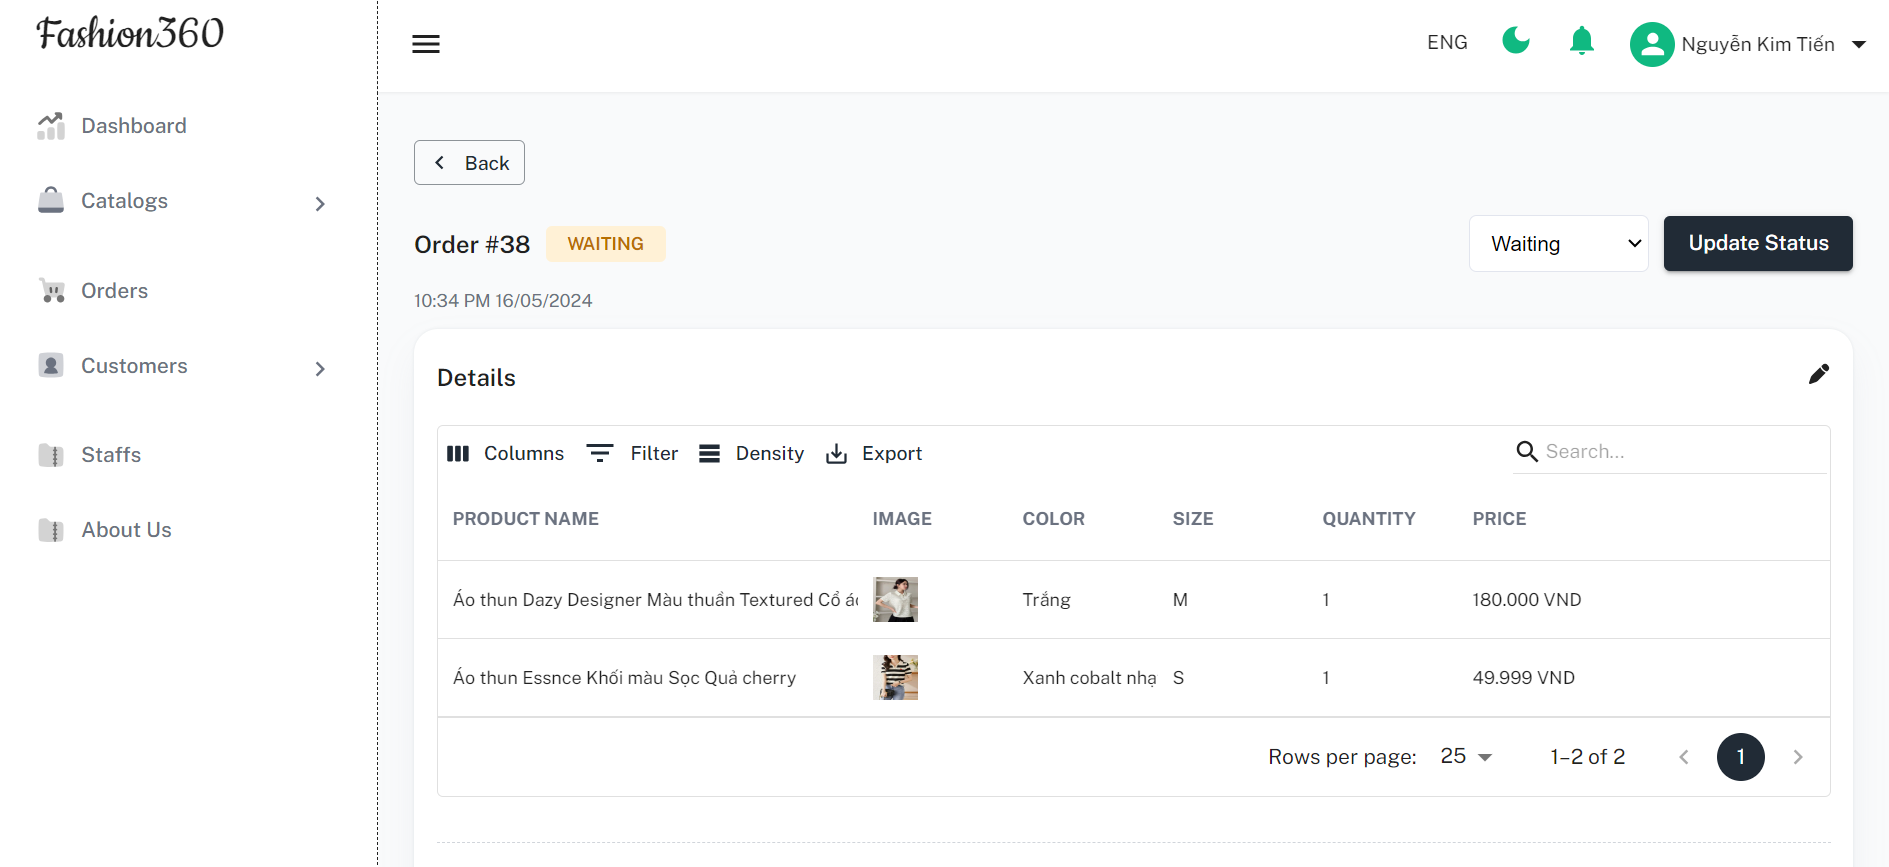
\includegraphics[width=14cm]{Images/Web/orderDetail1.png}
        \newline
        \caption{Một phần giao diện hiển thị thông tin chi tiết đơn hàng}
\end{figure}
\begin{figure}[H]
        \centering
        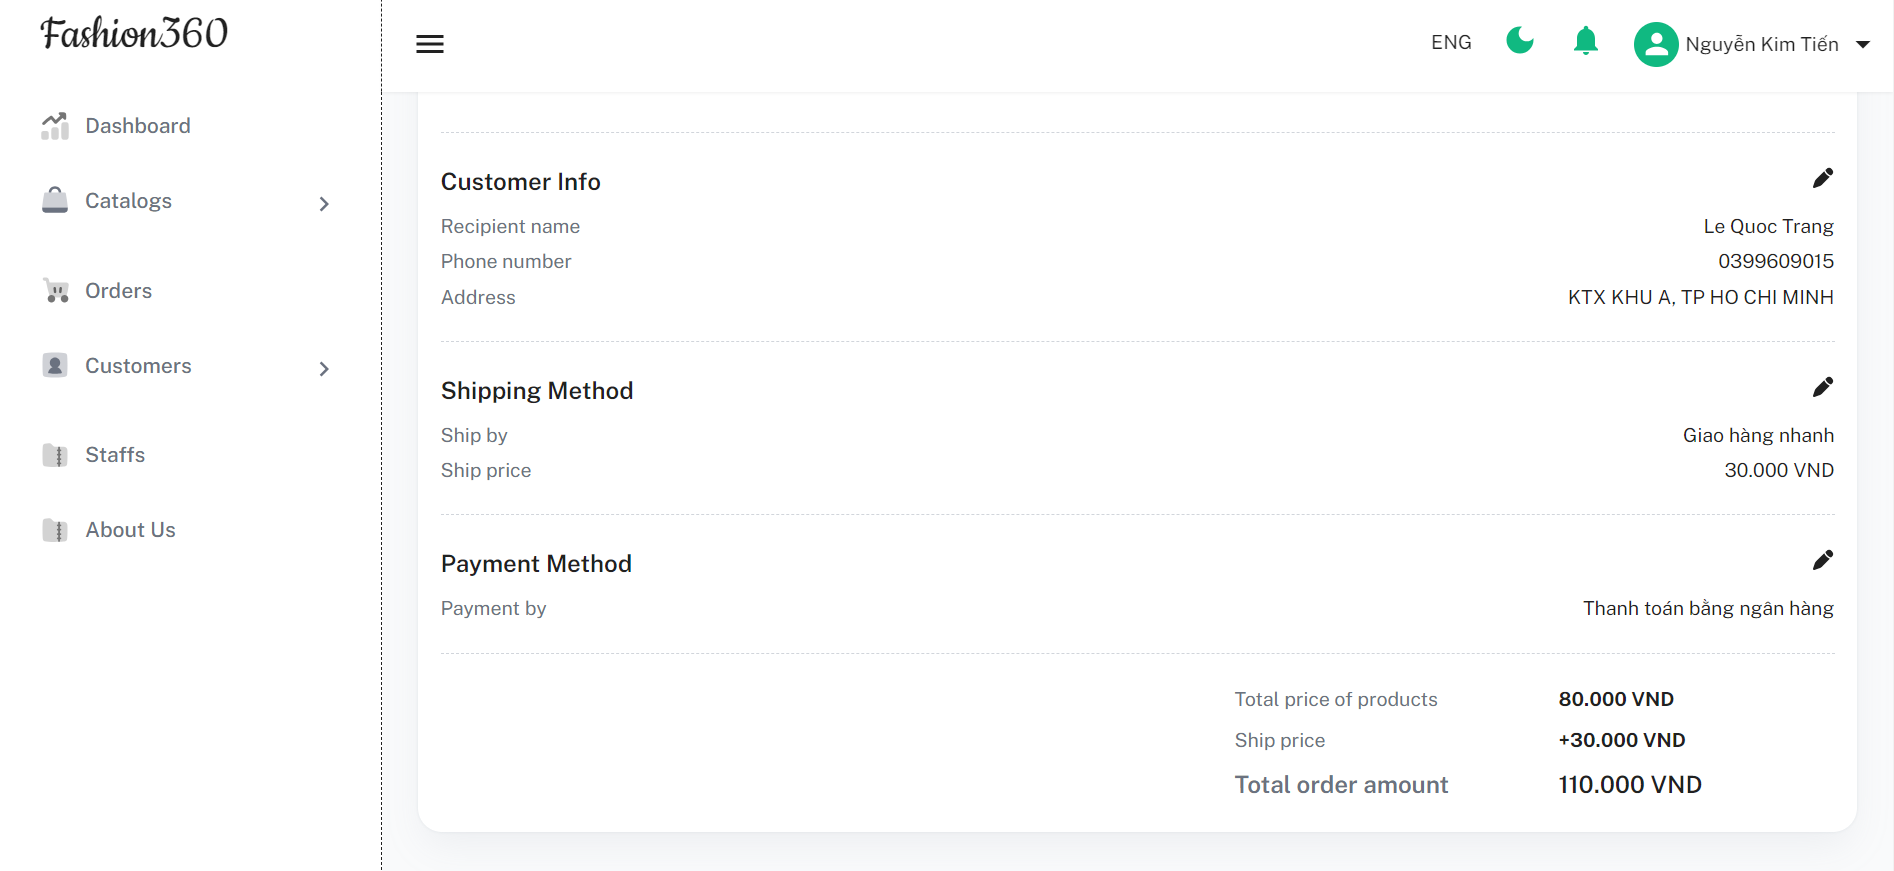
\includegraphics[width=14cm]{Images/Web/orderDetail2.png}
        \newline
        \caption{Một phần giao diện hiển thị thông tin chi tiết đơn hàng}
\end{figure}

\begin{itemize}
    \item \textbf{Trang Khách hàng (Customer)}
\end{itemize}

\begin{figure}[H]
        \centering
        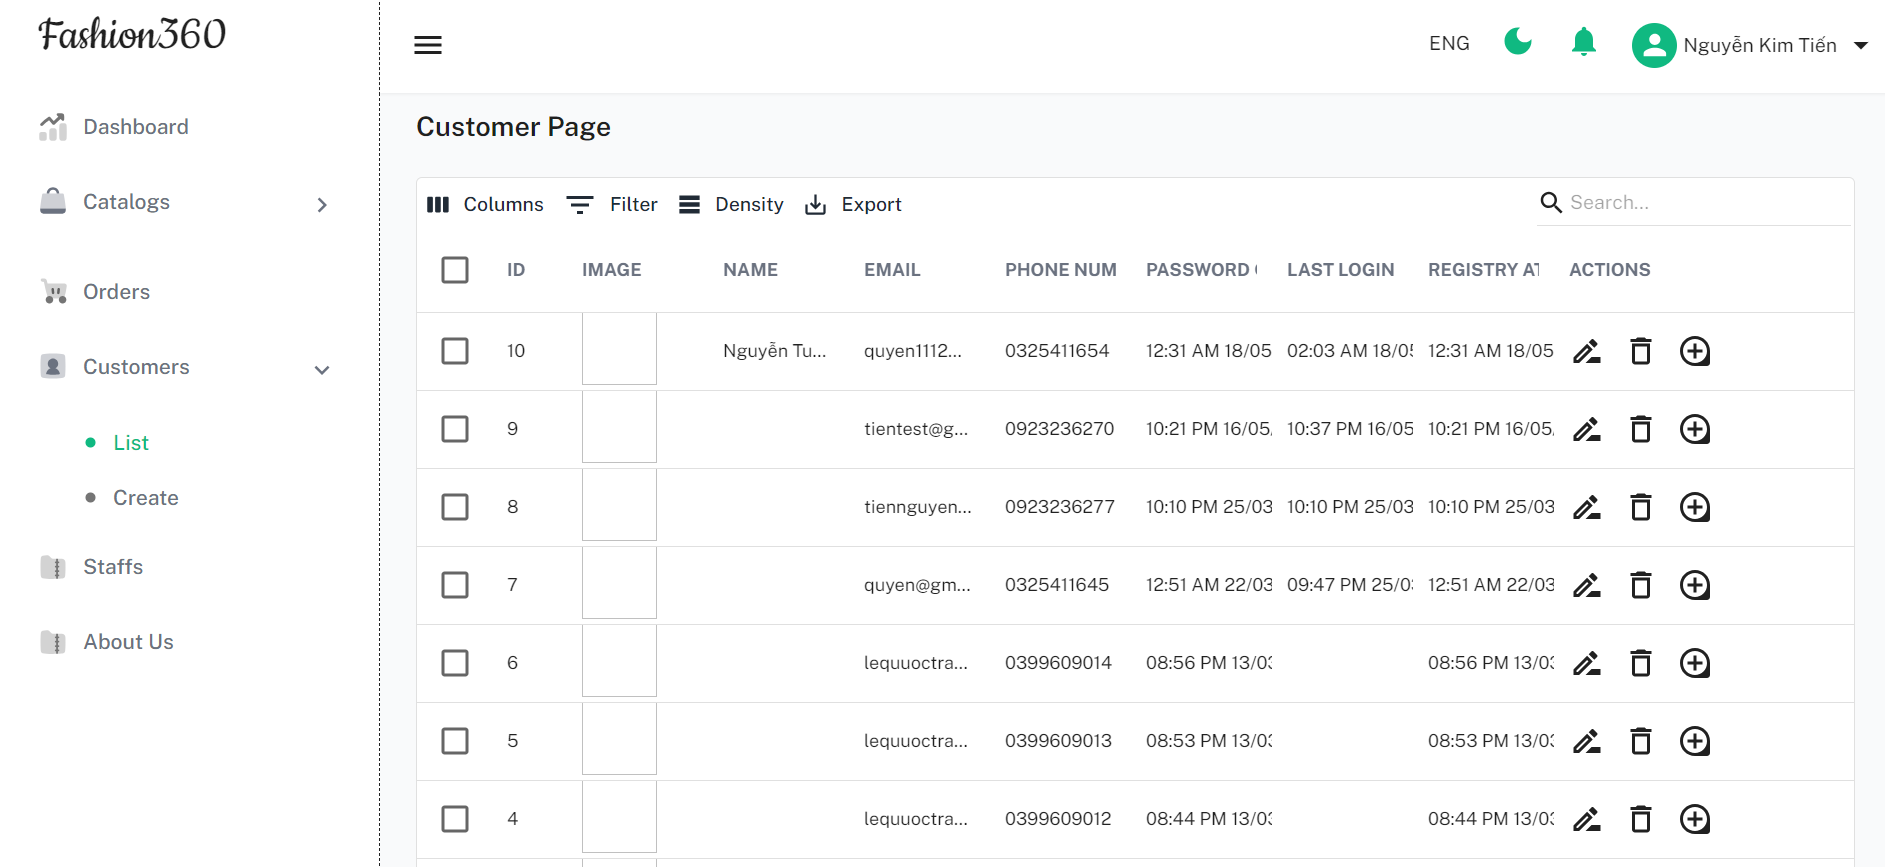
\includegraphics[width=14cm]{Images/Web/CustomerList.png}
        \newline
        \caption{Giao diện hiển thị danh sách khách hàng}
\end{figure}

\begin{figure}[H]
        \centering
        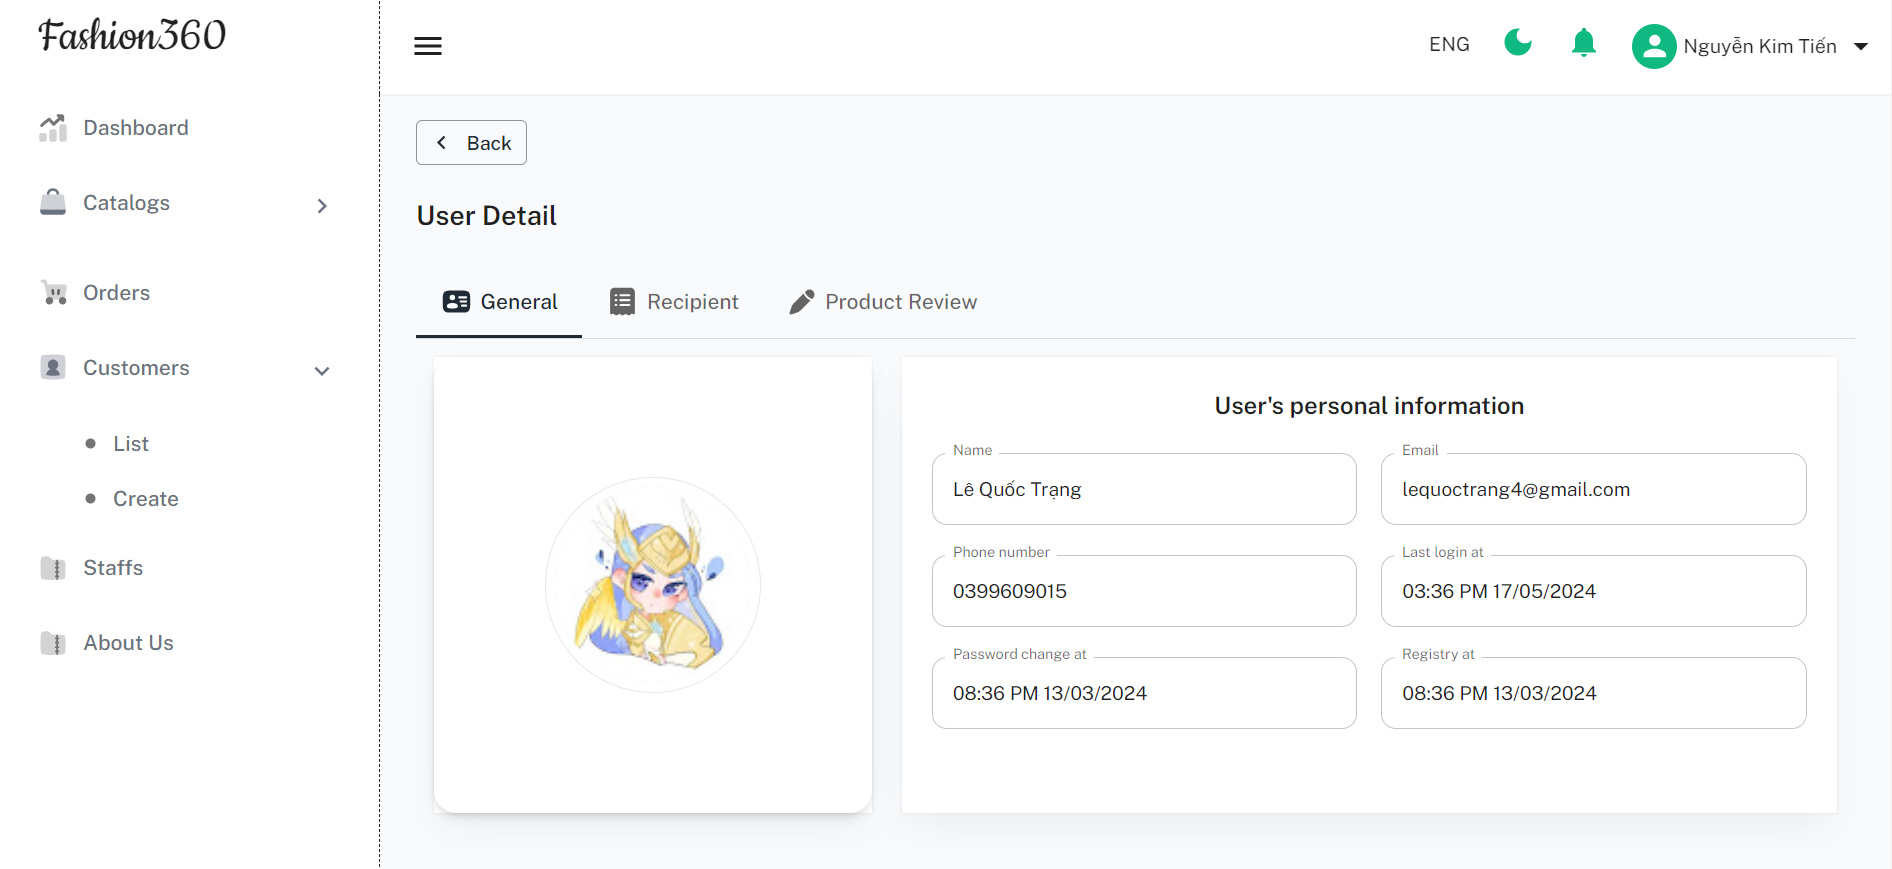
\includegraphics[width=14cm]{Images/Web/userDetail1.png}
        \newline
        \caption{Giao diện hiển thị thông tin cá nhân của khách hàng}
\end{figure}

\begin{figure}[H]
        \centering
        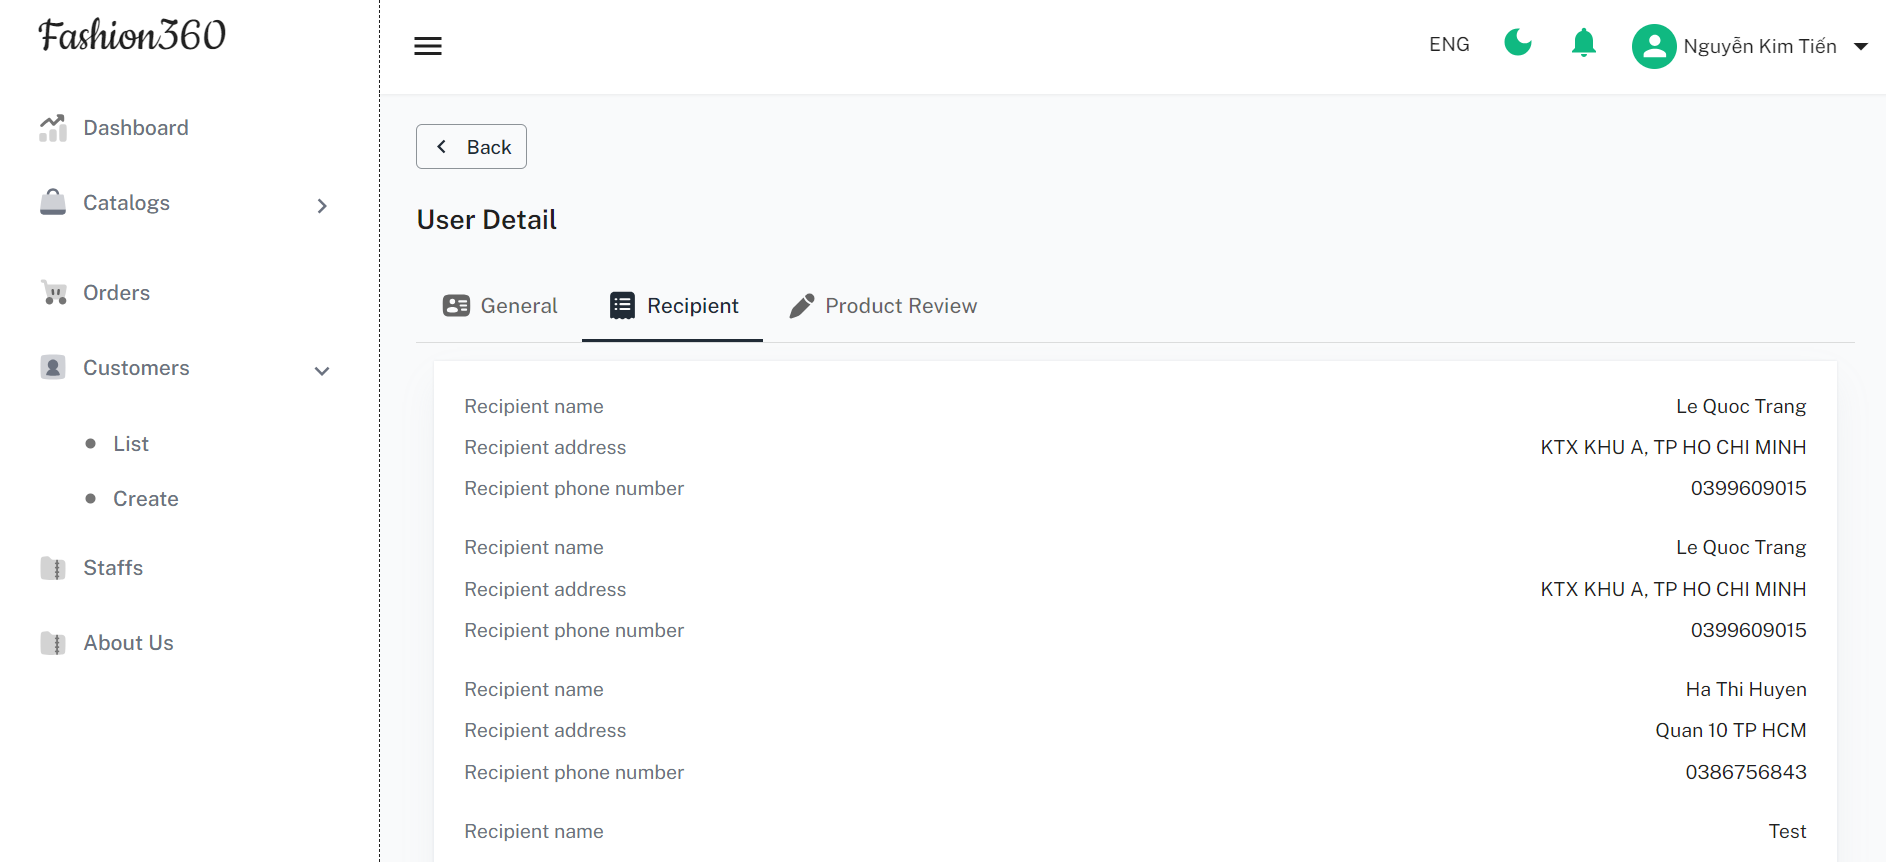
\includegraphics[width=14cm]{Images/Web/userDetail2.png}
        \newline
        \caption{Giao diện hiển thị thông tin nhận hàng của khách hàng}
\end{figure}

\begin{itemize}
    \item \textbf{Trang Nhân viên (Staff)}
\end{itemize}
\begin{figure}[H]
        \centering
        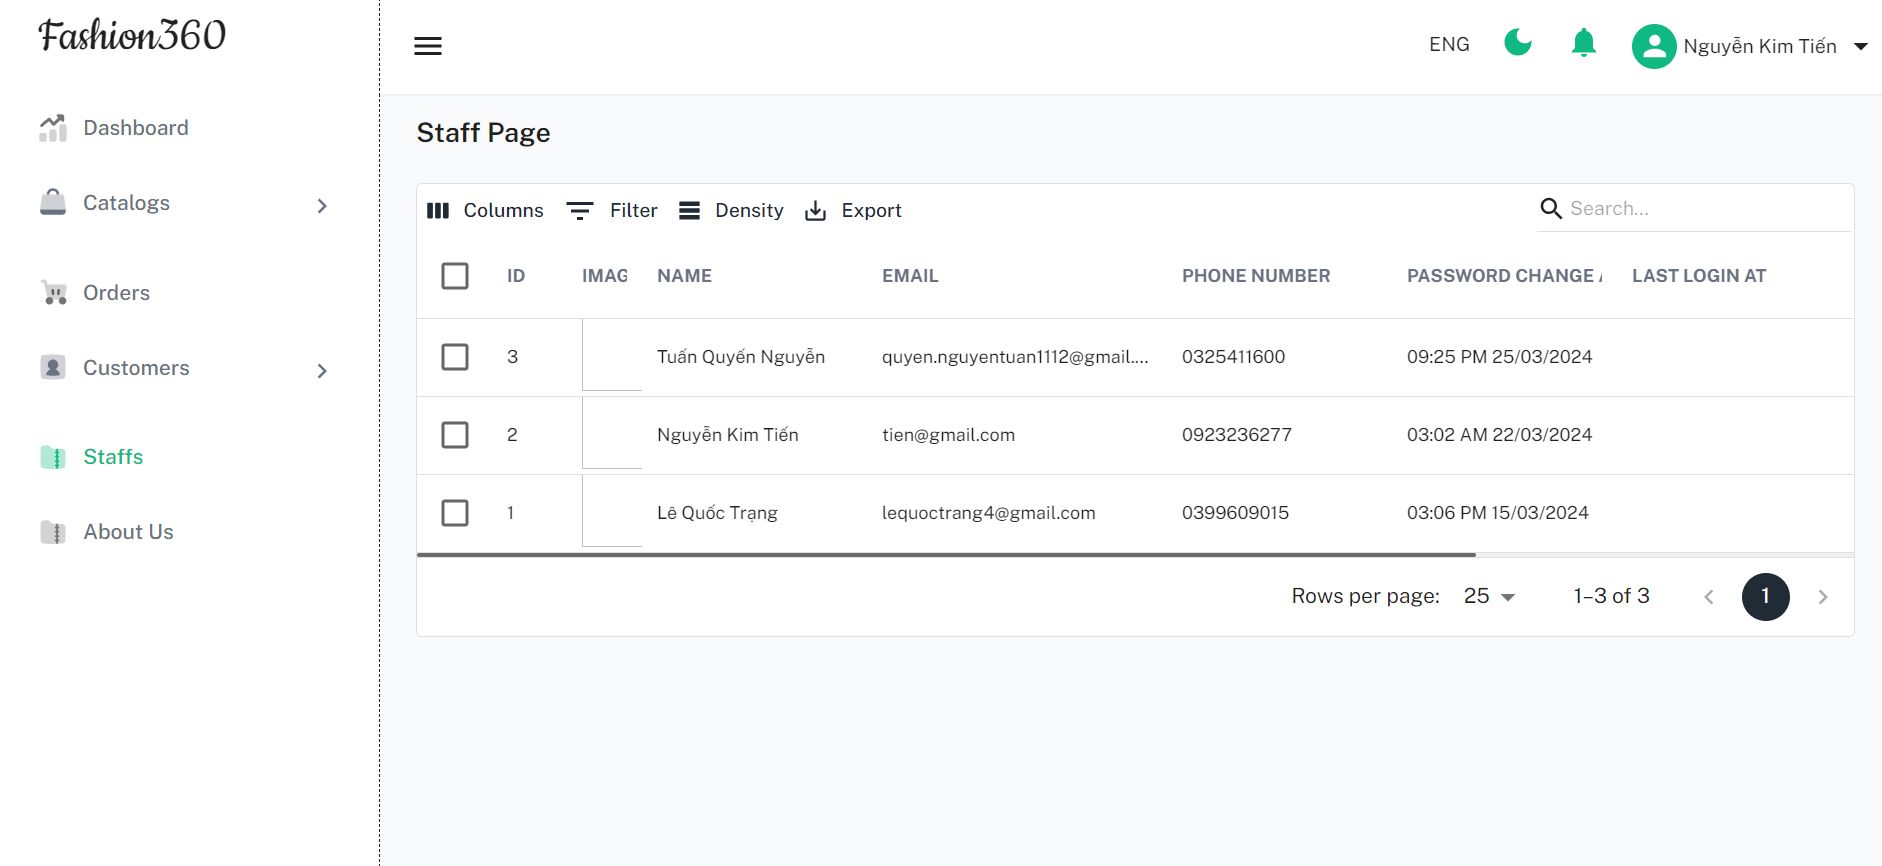
\includegraphics[width=14cm]{Images/Web/staffList.png}
        \newline
        \caption{Giao diện hiển thị danh sách nhân viên}
\end{figure}
\begin{figure}[H]
        \centering
        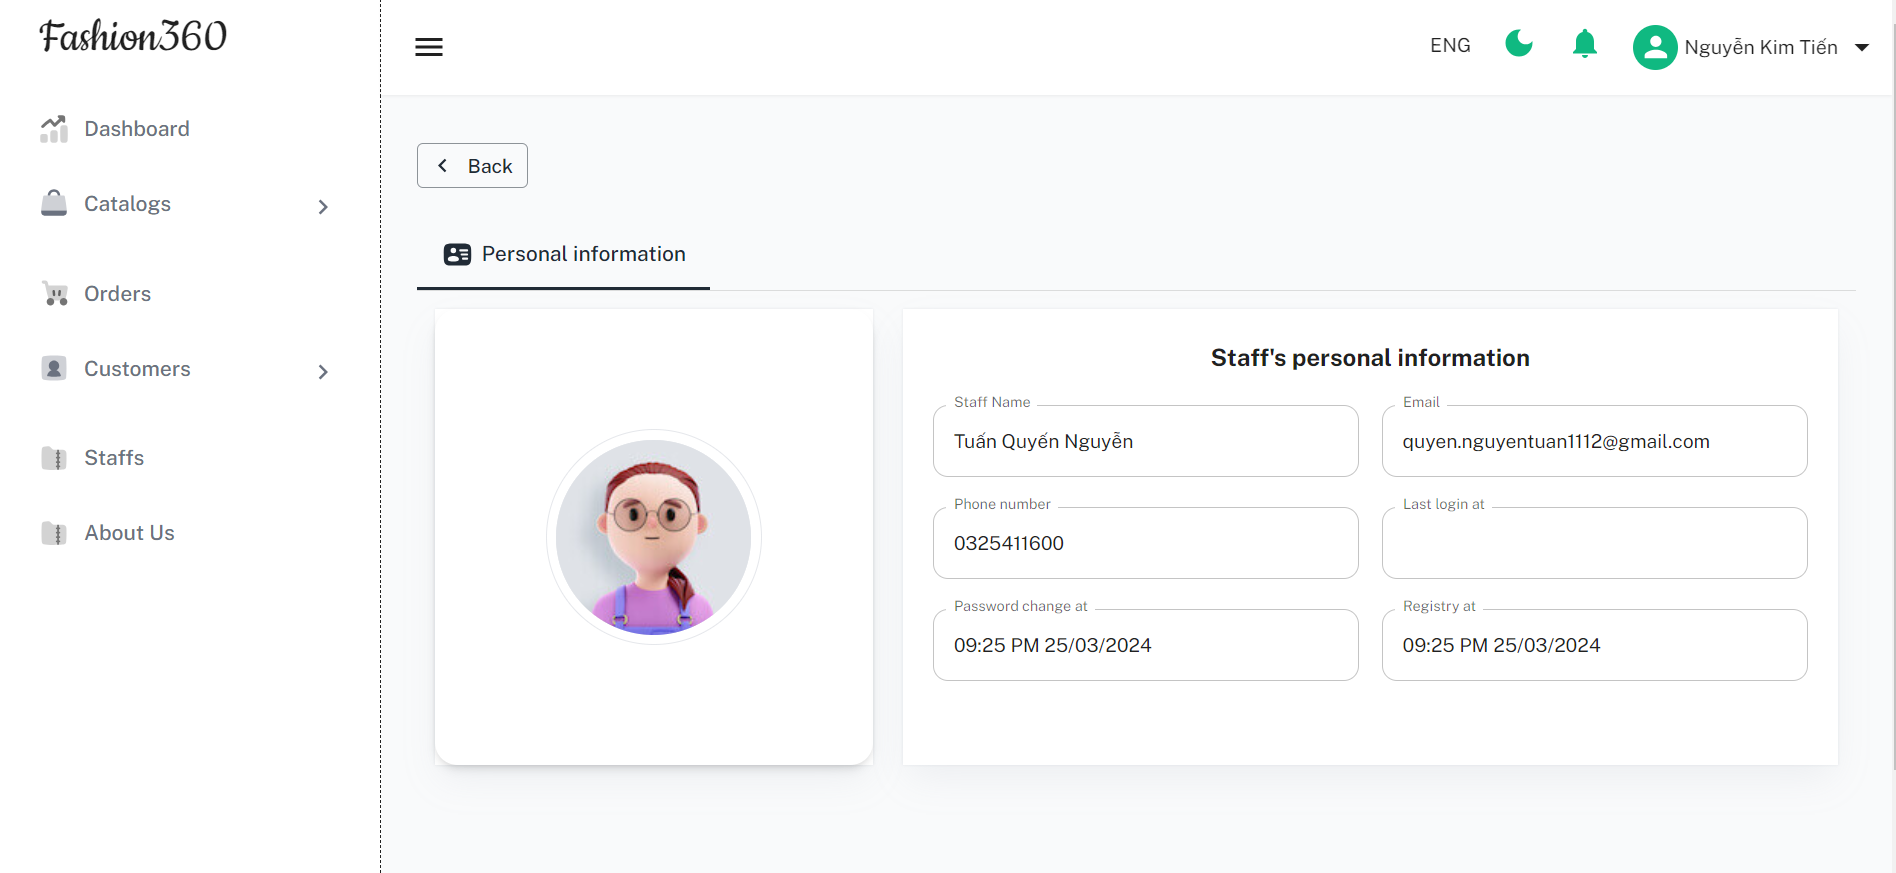
\includegraphics[width=14cm]{Images/Web/staffDetail.png}
        \newline
        \caption{Giao diện hiển thị thông tin cá nhân của nhân viên}
\end{figure}

\subsubsection{Giao diện ứng dụng di động của người dùng}

    \begin{figure}[H]
    \centering
    \begin{minipage}{0.45\textwidth}
        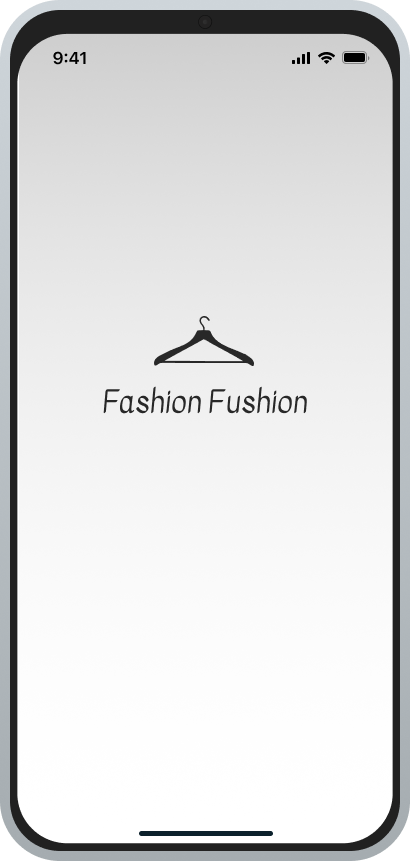
\includegraphics[scale=0.35]{Images/Design/User/GettingStarted/Launch screem.png}
        \vspace{10pt}
        \centering
        \caption{Khởi động ứng dụng}
    \end{minipage}\hfill
    \begin{minipage}{0.45\textwidth}
        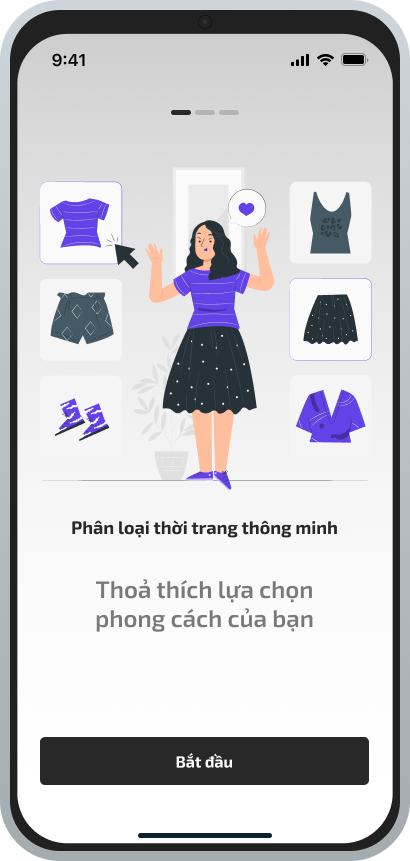
\includegraphics[scale=0.35]{Images/Design/User/GettingStarted/Onboarding.png}
        \vspace{10pt}
        \centering
        \caption{Giới thiệu}
    \end{minipage}
    \end{figure}

     \begin{figure}[H]
    \centering
    \begin{minipage}{0.45\textwidth}
        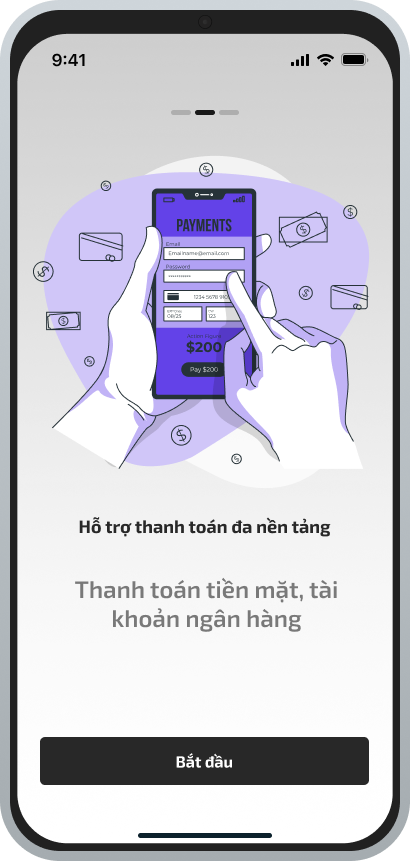
\includegraphics[scale=0.35]{Images/Design/User/GettingStarted/Onboarding (1).png}
        \vspace{10pt}
        \centering
        \caption{Giới thiệu}
    \end{minipage}\hfill
    \begin{minipage}{0.45\textwidth}
        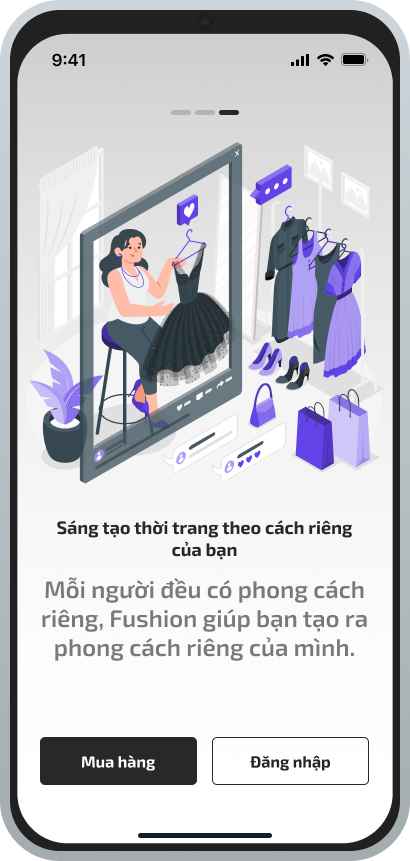
\includegraphics[scale=0.35]{Images/Design/User/GettingStarted/Get started.png}
        \vspace{10pt}
        \centering
        \caption{Giới thiệu}
    \end{minipage}
    \end{figure}

    % Author

      \begin{figure}[H]
    \centering
    \begin{minipage}{0.45\textwidth}
        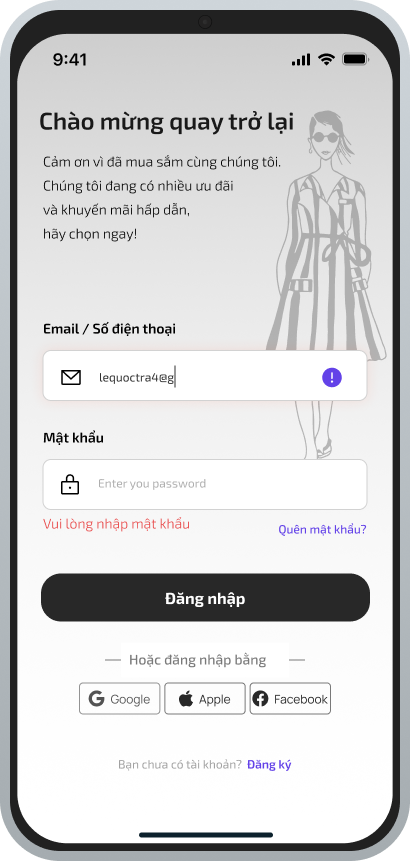
\includegraphics[scale=0.35]{Images/Design/User/Author/SignIn.png}
        \vspace{10pt}
        \centering \caption{Đăng nhập}
    \end{minipage}\hfill
    \begin{minipage}{0.45\textwidth}
        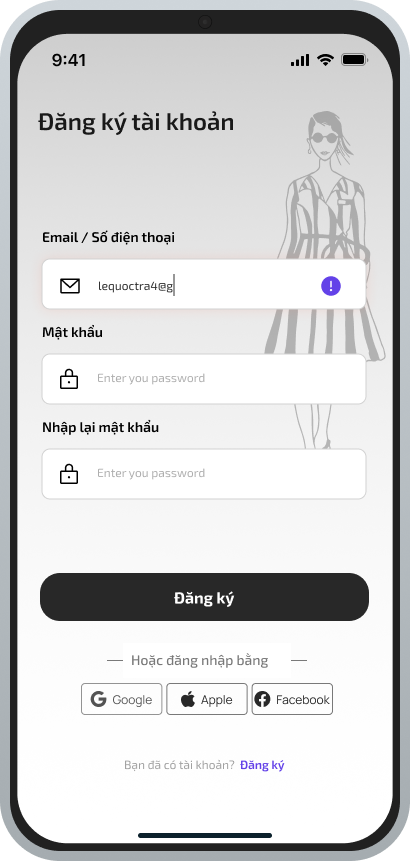
\includegraphics[scale=0.35]{Images/Design/User/Author/SignUp.png}
        \vspace{10pt}
        \centering \caption{Đăng ký tài khoản}
    \end{minipage}
    \end{figure}

      \begin{figure}[H]
    \centering
    \begin{minipage}{0.45\textwidth}
        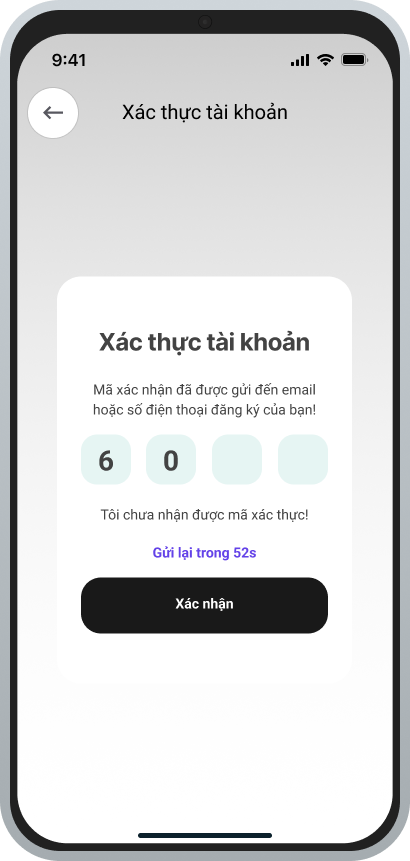
\includegraphics[scale=0.35]{Images/Design/User/Author/Xác thực.png}
        \vspace{10pt}
        \centering \caption{Nhập mã xác thực tài khoản}
    \end{minipage}\hfill
    \begin{minipage}{0.45\textwidth}
        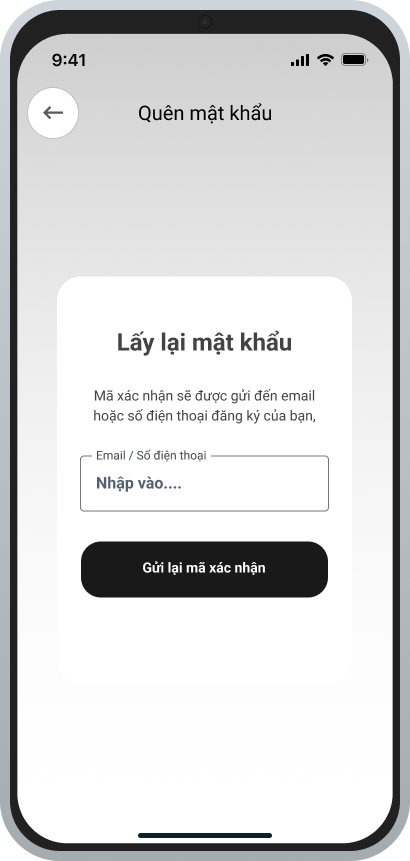
\includegraphics[scale=0.35]{Images/Design/User/Author/Quên mật khẩu.png}
        \vspace{10pt}
        \centering \caption{Lấy lại mật khẩu}
    \end{minipage}
    \end{figure}

      \begin{figure}[H]
    \centering
    \begin{minipage}{0.45\textwidth}
        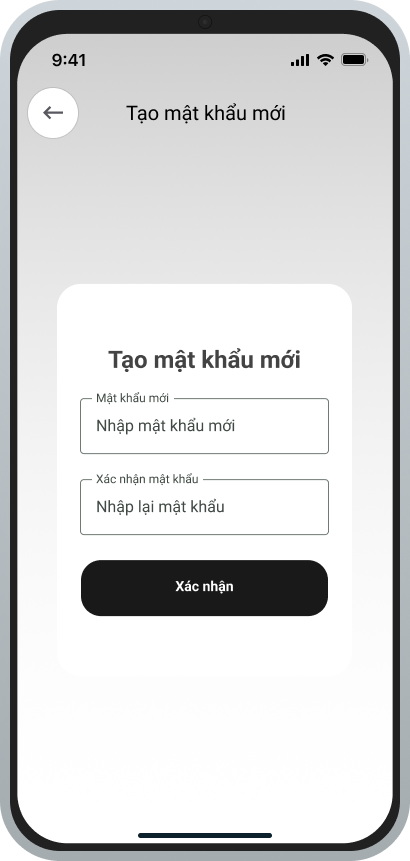
\includegraphics[scale=0.35]{Images/Design/User/Author/Tạo mật khẩu mới 1.png}
        \vspace{10pt}
        \centering \caption{Tạo mật khẩu mới}
    \end{minipage}\hfill
    \begin{minipage}{0.45\textwidth}
        \includegraphics[width=5cm]{{Images/Design/User/Main/Search.png}}
        \vspace{10pt}
        \centering \caption{Tìm kiếm sản phẩm}
    \end{minipage}
    \end{figure}


    \begin{figure}[H]
    \centering
    \begin{minipage}{0.45\textwidth}
        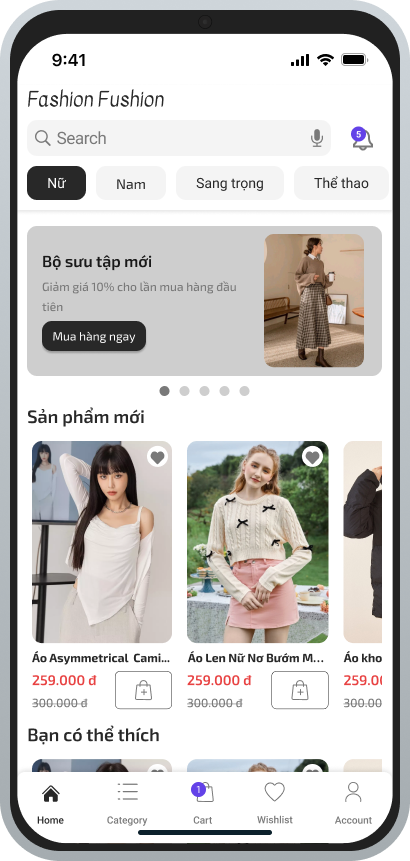
\includegraphics[scale=0.35]{Images/Design/User/Main/HomePage.png}
        \vspace{10pt}
        \centering \caption{Trang chủ}
    \end{minipage}\hfill
    \begin{minipage}{0.45\textwidth}
        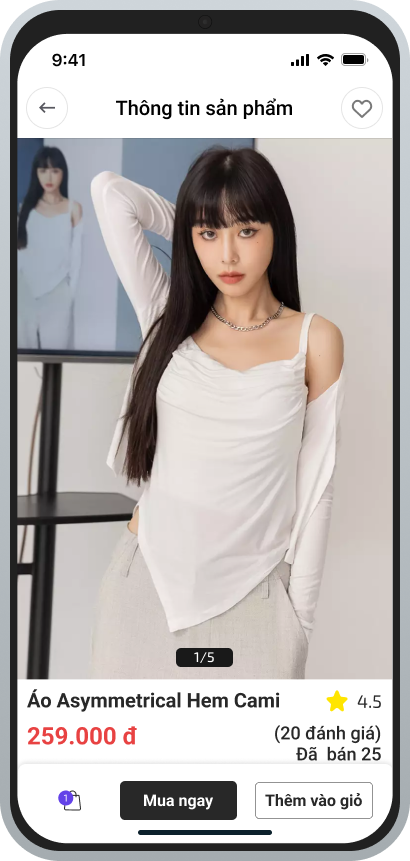
\includegraphics[scale=0.35]{Images/Design/User/Main/Product Detail.png}
        \vspace{10pt}
        \centering \caption{Thông tin sản phẩm}
    \end{minipage}
    \end{figure}

      \begin{figure}[H]
    \centering
    \begin{minipage}{0.45\textwidth}
        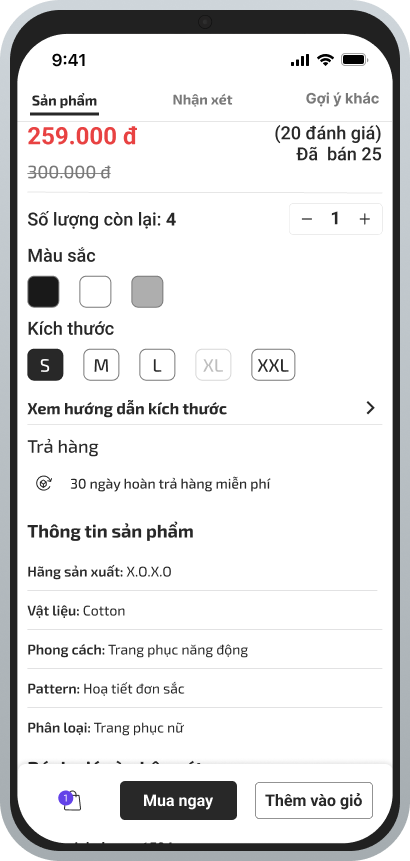
\includegraphics[scale=0.35]{Images/Design/User/Main/Product Detail-1.png}
        \vspace{10pt}
        \centering \caption{Thông tin chi tiết sản phẩm}
    \end{minipage}\hfill
    \begin{minipage}{0.45\textwidth}
        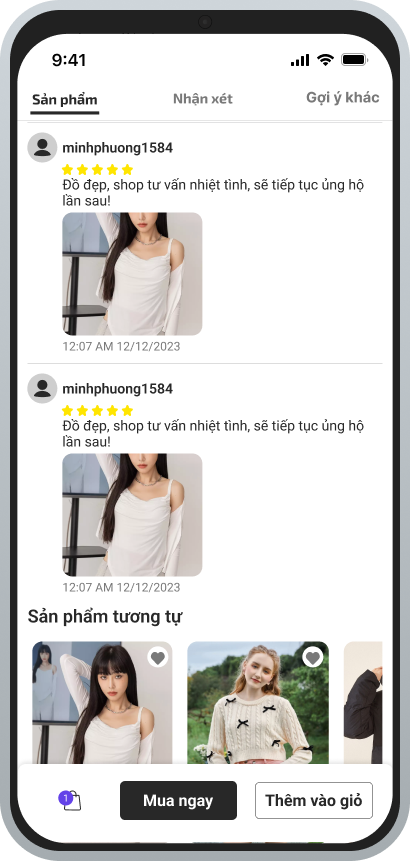
\includegraphics[scale=0.35]{Images/Design/User/Main/Product Detail-2.png}
        \vspace{10pt}
        \centering \caption{Xem đánh giá về sản phẩm}
    \end{minipage}
    \end{figure}

      \begin{figure}[H]
    \centering
    \begin{minipage}{0.45\textwidth}
        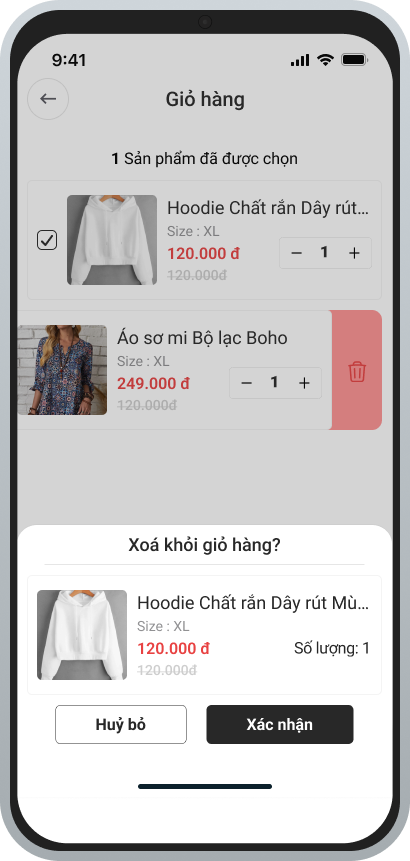
\includegraphics[scale=0.35]{Images/Design/User/Main/Giỏ hàng.png}
        \vspace{10pt}
        \centering \caption{Xóa sản phẩm khỏi giỏ hàng}
    \end{minipage}\hfill
    \begin{minipage}{0.45\textwidth}
        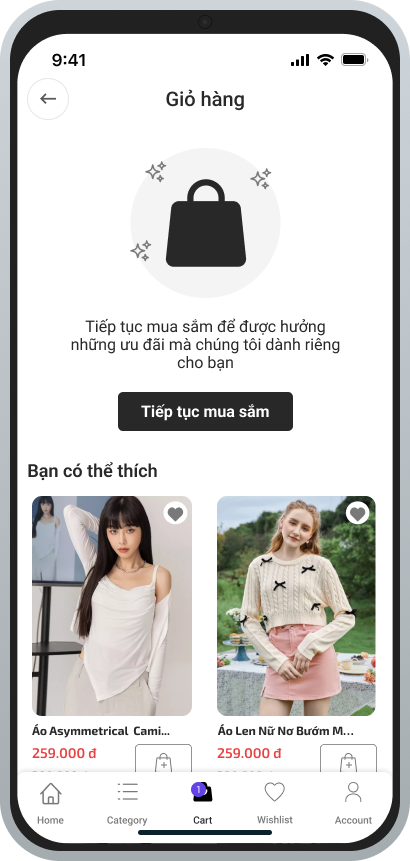
\includegraphics[scale=0.35]{Images/Design/User/Main/Giỏ hàng-1.png}
        \vspace{10pt}
        \centering \caption{Xem giỏ hàng}
    \end{minipage}
    \end{figure}

      \begin{figure}[H]
    \centering
    \begin{minipage}{0.45\textwidth}
        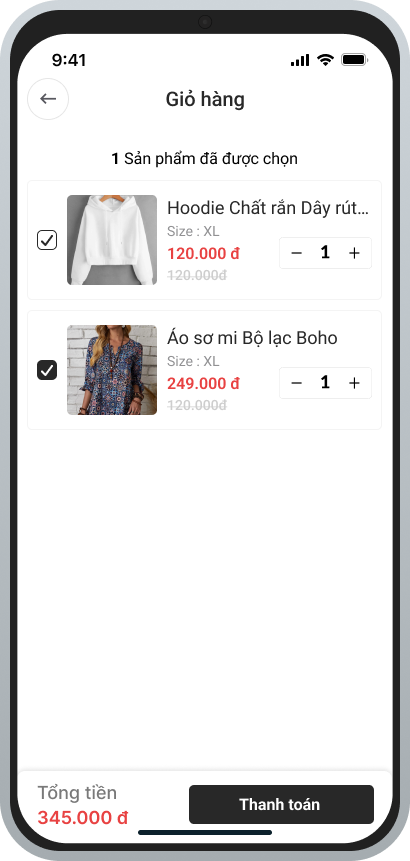
\includegraphics[scale=0.35]{Images/Design/User/Main/Giỏ hàng-2.png}
        \vspace{10pt}
        \centering \caption{Chỉnh sửa giỏ hàng }
    \end{minipage}\hfill
    \begin{minipage}{0.45\textwidth}
        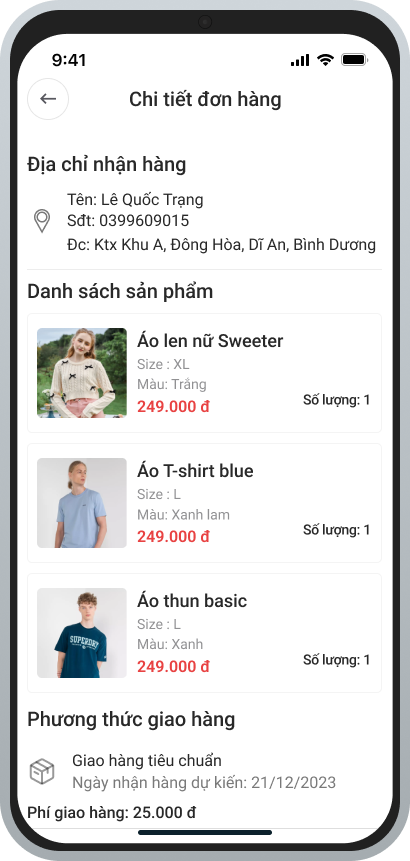
\includegraphics[scale=0.35]{Images/Design/User/Main/Order detail.png}
        \vspace{10pt}
        \centering \caption{Chi tiết đơn hàng}
    \end{minipage}
    \end{figure}

      \begin{figure}[H]
    \centering
    \begin{minipage}{0.45\textwidth}
        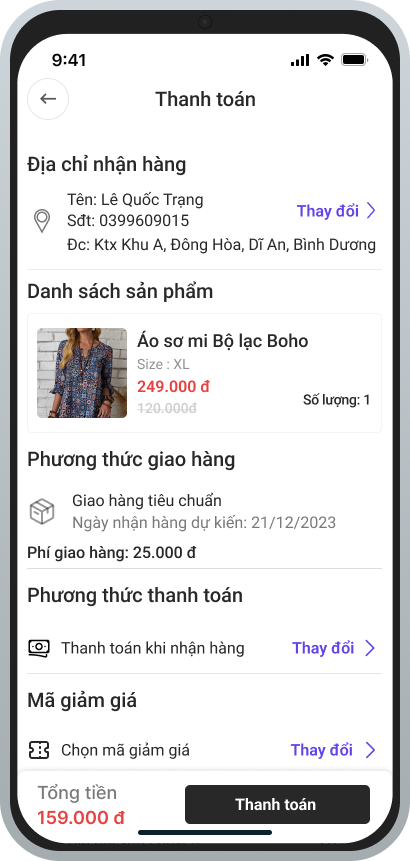
\includegraphics[scale=0.35]{Images/Design/User/Main/Thanh toán.png}
        \vspace{10pt}
        \centering \caption{Thanh toán đơn hàng}
    \end{minipage}\hfill
    \begin{minipage}{0.45\textwidth}
        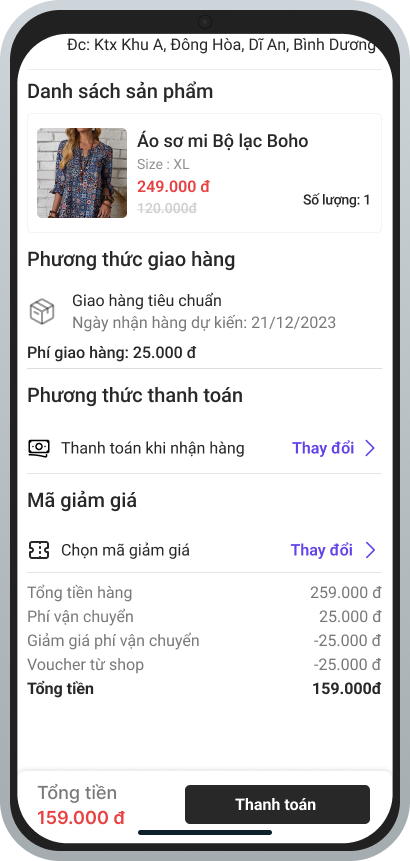
\includegraphics[scale=0.35]{Images/Design/User/Main/Thanh toán-1.png}
        \vspace{10pt}
        \centering \caption{Thanh toán đơn hàng}
    \end{minipage}
    \end{figure}

      \begin{figure}[H]
    \centering
    \begin{minipage}{0.45\textwidth}
        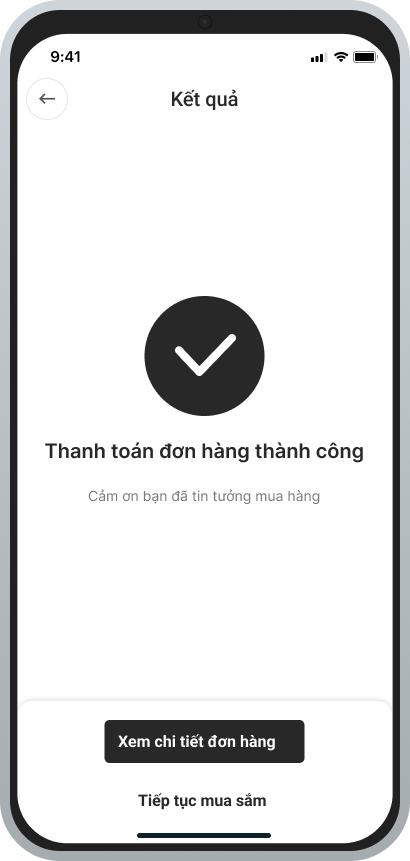
\includegraphics[scale=0.35]{Images/Design/User/Main/Payment Success.png}
        \vspace{10pt}
        \centering \caption{Thanh toán đơn hàng thành công}
    \end{minipage}\hfill
    \begin{minipage}{0.45\textwidth}
        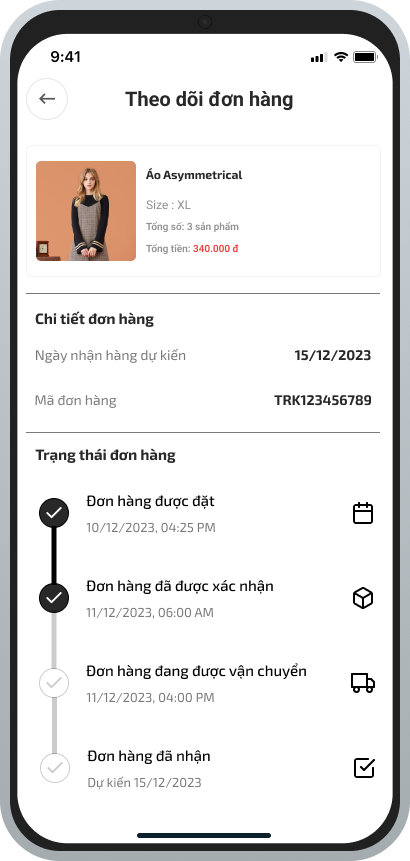
\includegraphics[scale=0.35]{Images/Design/User/Main/Track order.png}
        \vspace{10pt}
        \centering \caption{Theo dõi đơn hàng}
    \end{minipage}
    \end{figure}

      \begin{figure}[H]
    \centering
    \begin{minipage}{0.45\textwidth}
        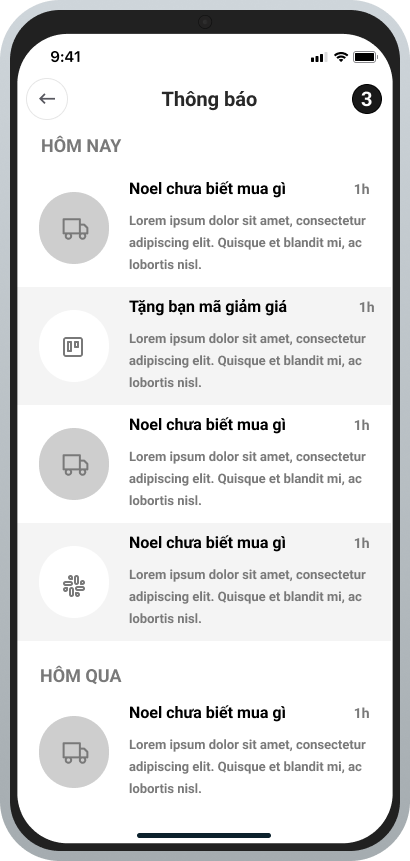
\includegraphics[scale=0.35]{Images/Design/User/Main/Thông báo.png}
        \vspace{10pt}
        \centering \caption{Xem thông báo}
    \end{minipage}\hfill
    \begin{minipage}{0.45\textwidth}
        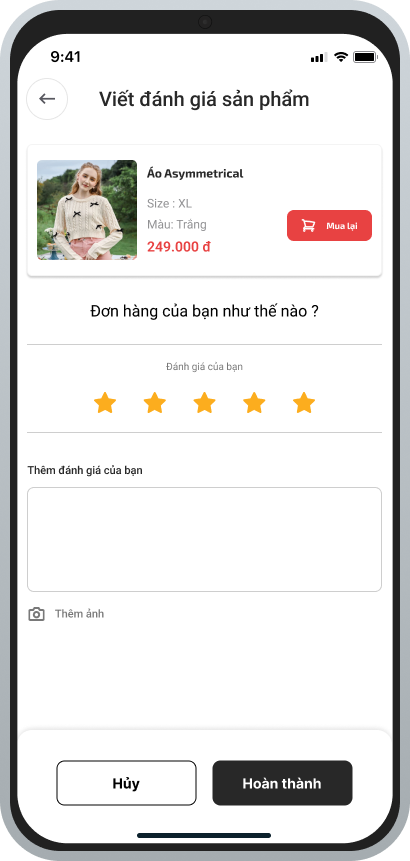
\includegraphics[scale=0.35]{Images/Design/User/Main/Viết đánh giá.png}
        \vspace{10pt}
        \centering \caption{Viết đánh giá sản phẩm}
    \end{minipage}
    \end{figure}

      \begin{figure}[H]
    \centering
    \begin{minipage}{0.45\textwidth}
        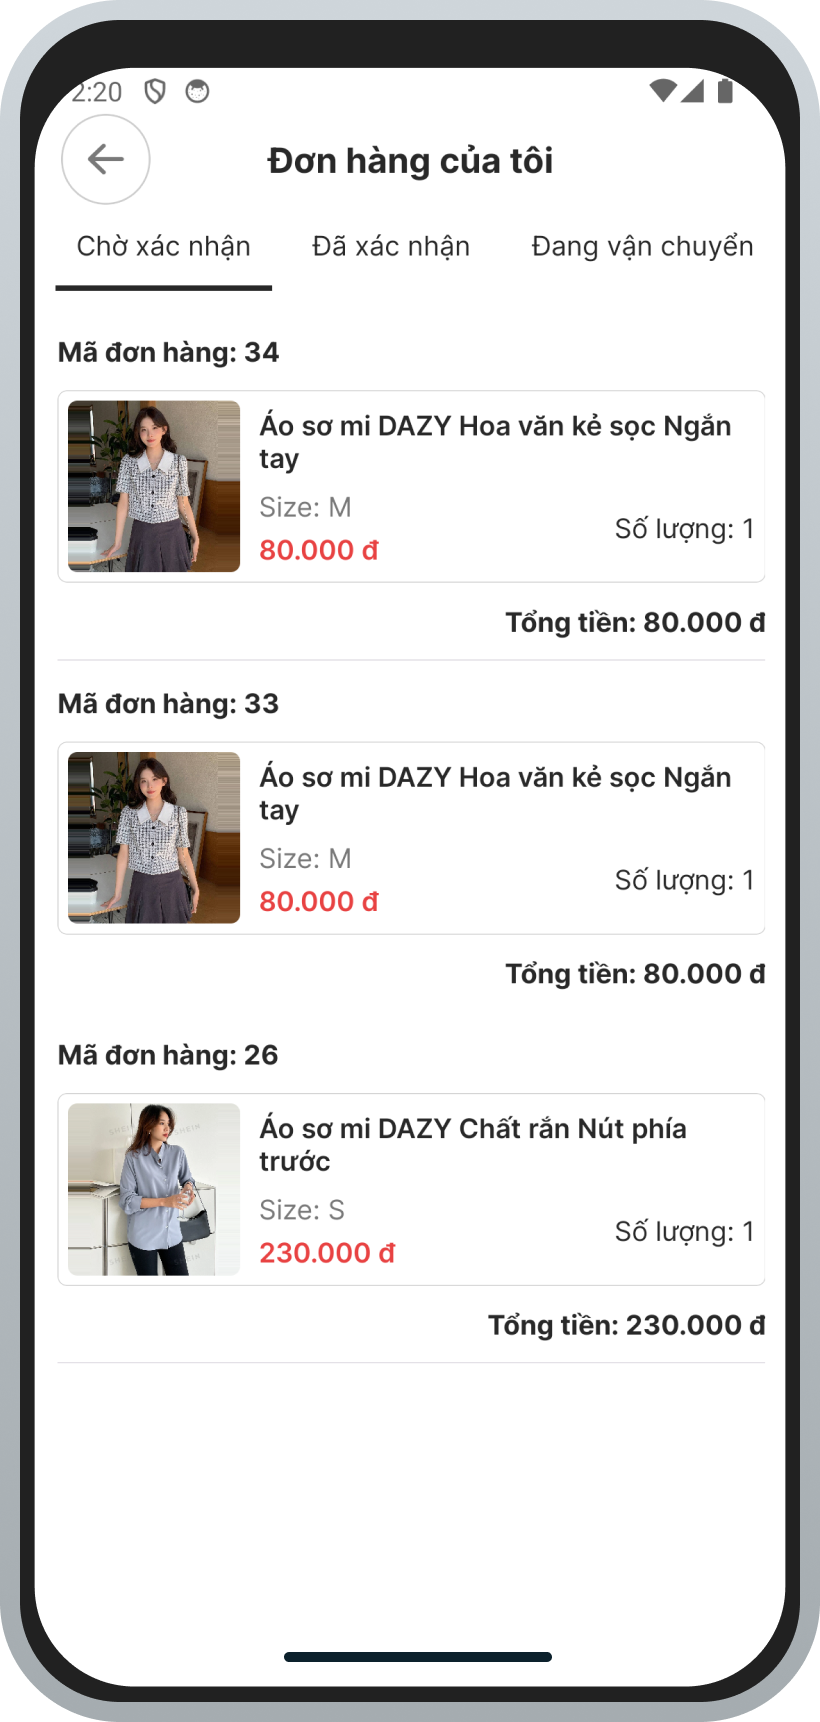
\includegraphics[width=5cm]{Images/Design/User/Main/order-status.png}
        \vspace{10pt}
        \centering \caption{Trạng thái đơn hàng}
    \end{minipage}\hfill
    \begin{minipage}{0.45\textwidth}
 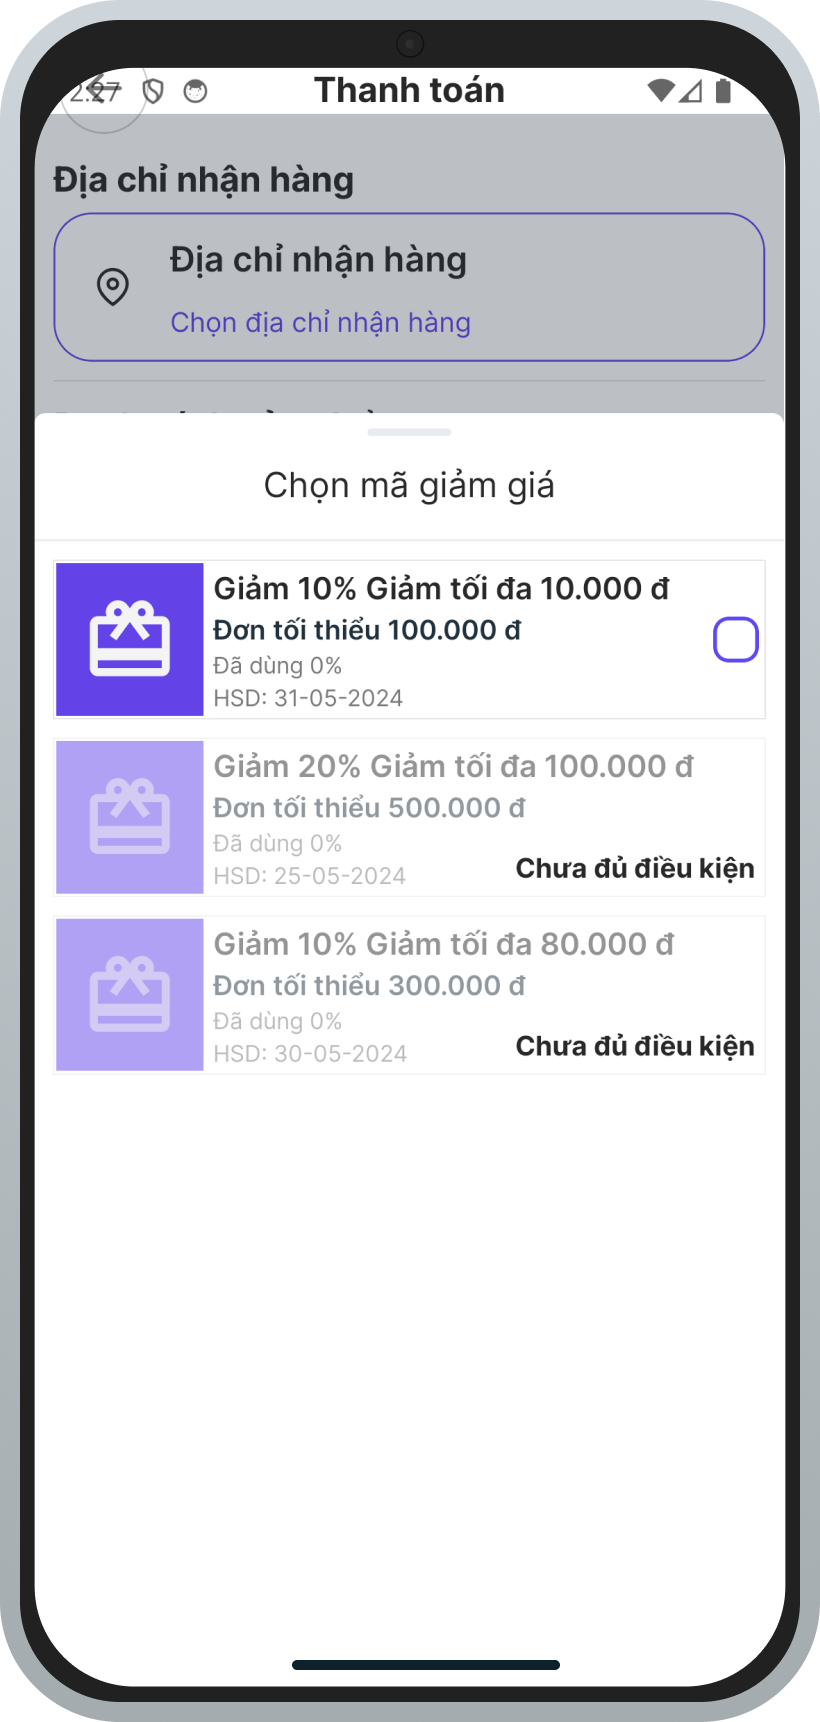
\includegraphics[width=5cm]{Images/Design/User/Main/Mã giảm giá.png}
        \vspace{10pt}
        \centering \caption{Nhập mã giảm giá}
    \end{minipage}
    \end{figure}


      \begin{figure}[H]
    \centering
    \begin{minipage}{0.45\textwidth}
        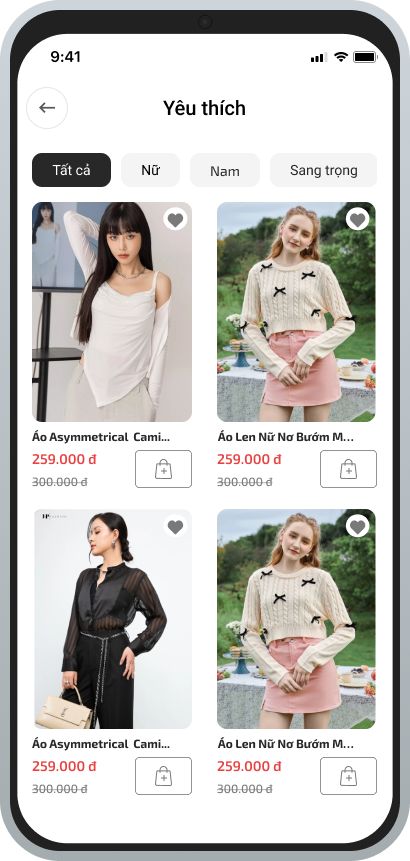
\includegraphics[scale=0.35]{Images/Design/User/Main/Wishlist.png}
        \vspace{10pt}
        \centering \caption{Sản phẩm yêu thích}
    \end{minipage}\hfill
    \begin{minipage}{0.45\textwidth}
        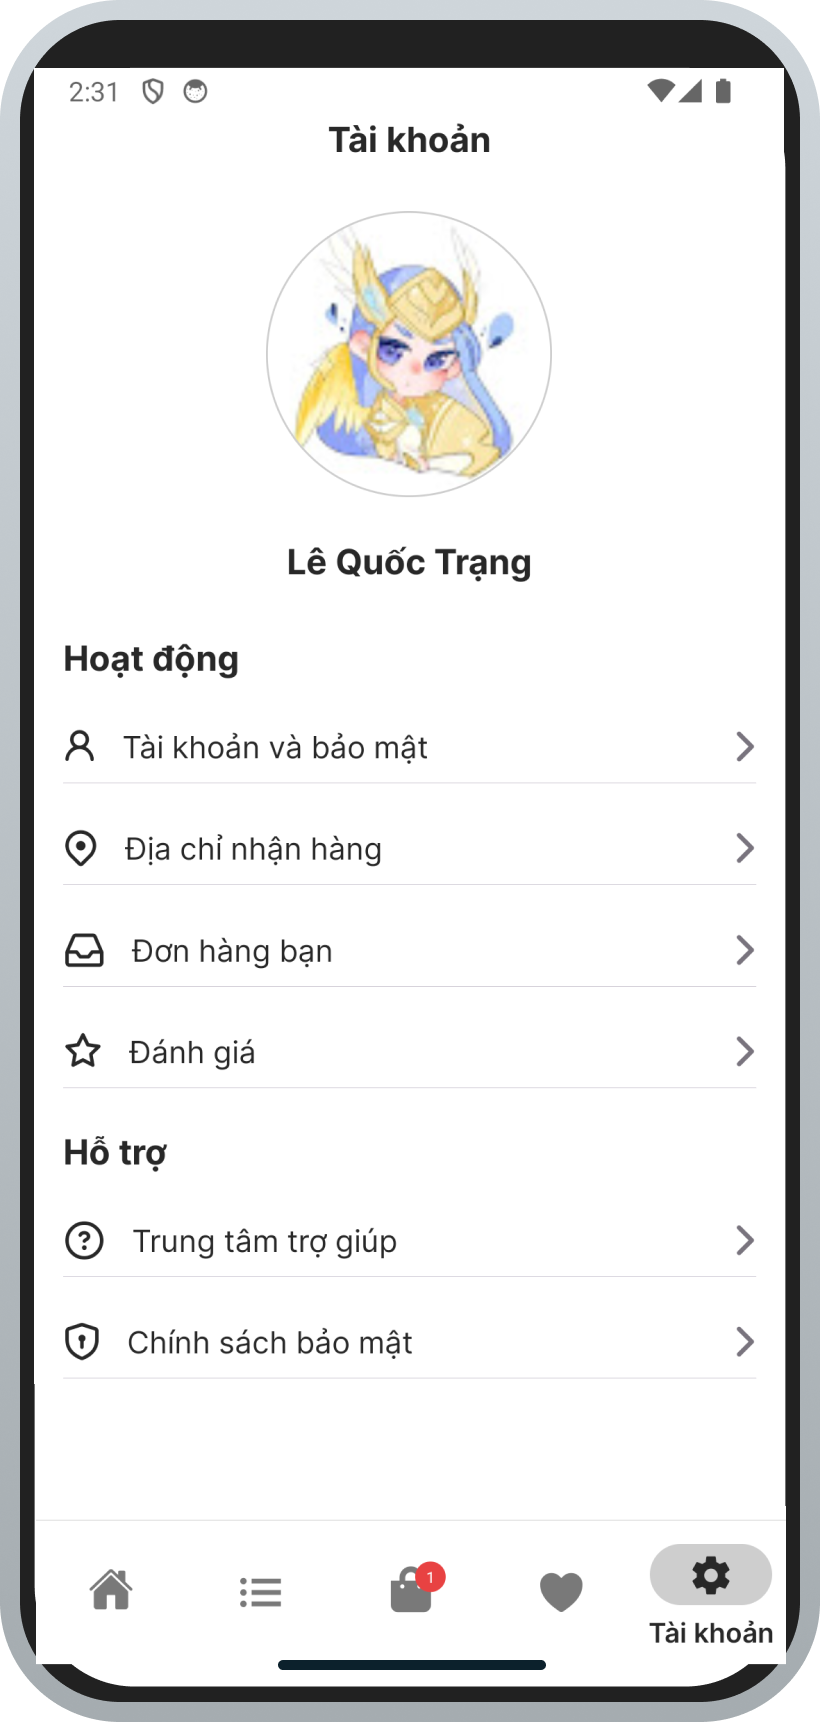
\includegraphics[width=5cm]{Images/Design/User/Main/Profile.png}
        \vspace{10pt}
        \centering \caption{Trang tài khoản}
    \end{minipage}
    \end{figure}

      \begin{figure}[H]
    \centering
    \begin{minipage}{0.45\textwidth}
        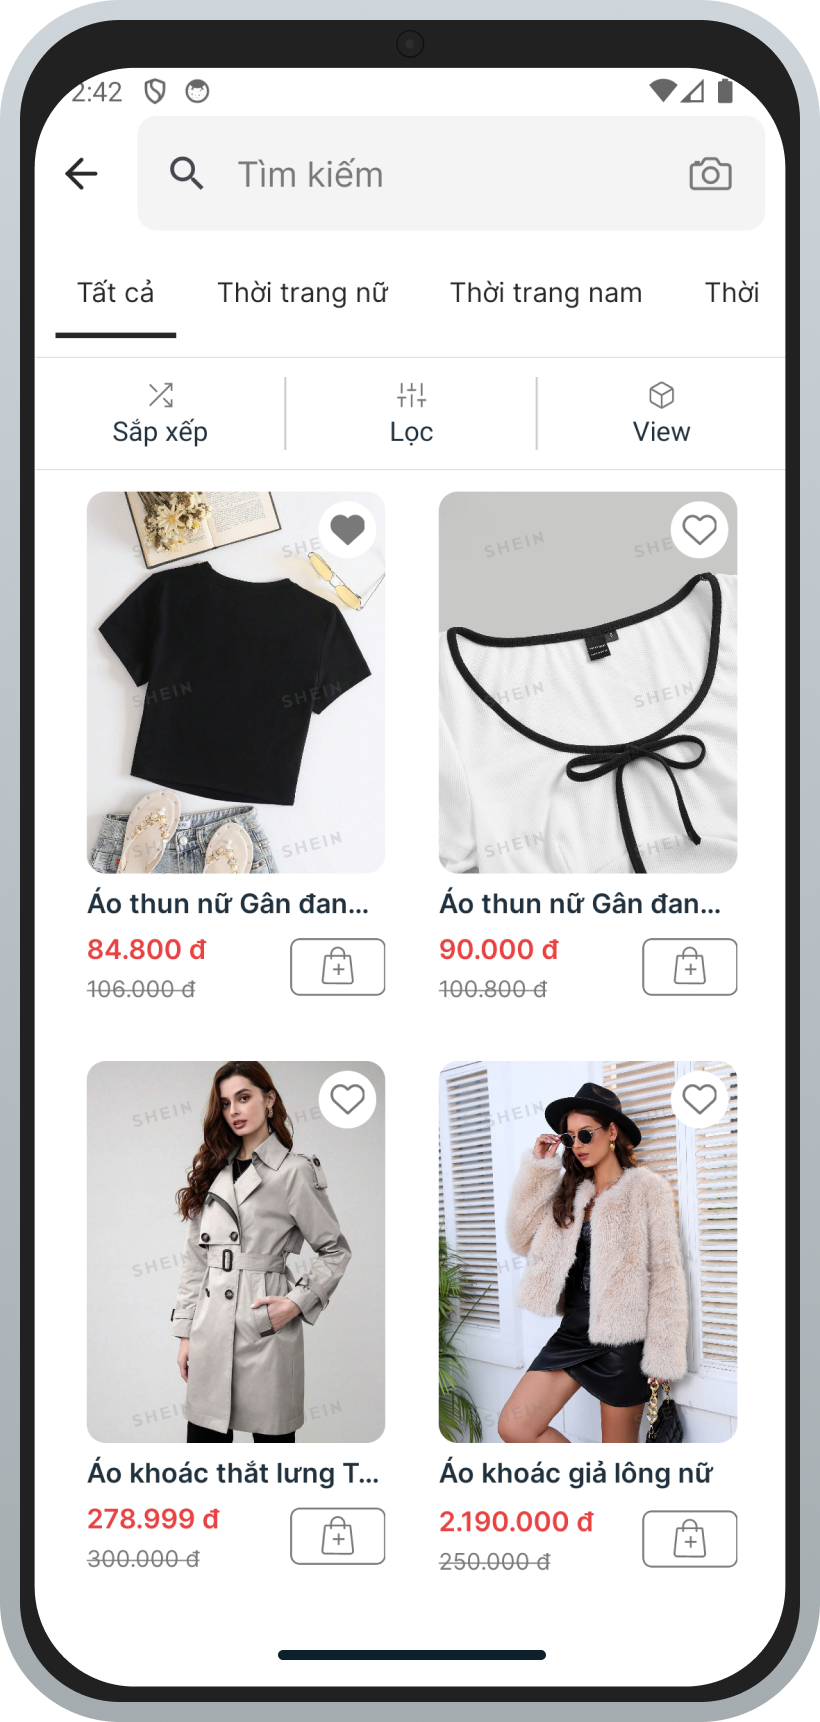
\includegraphics[width=5cm]{Images/Design/User/Main/Filter.png}
        \vspace{10pt}
        \centering \caption{Tìm kiếm, lọc, xem sản phẩm}
    \end{minipage}\hfill
    \begin{minipage}{0.45\textwidth}
        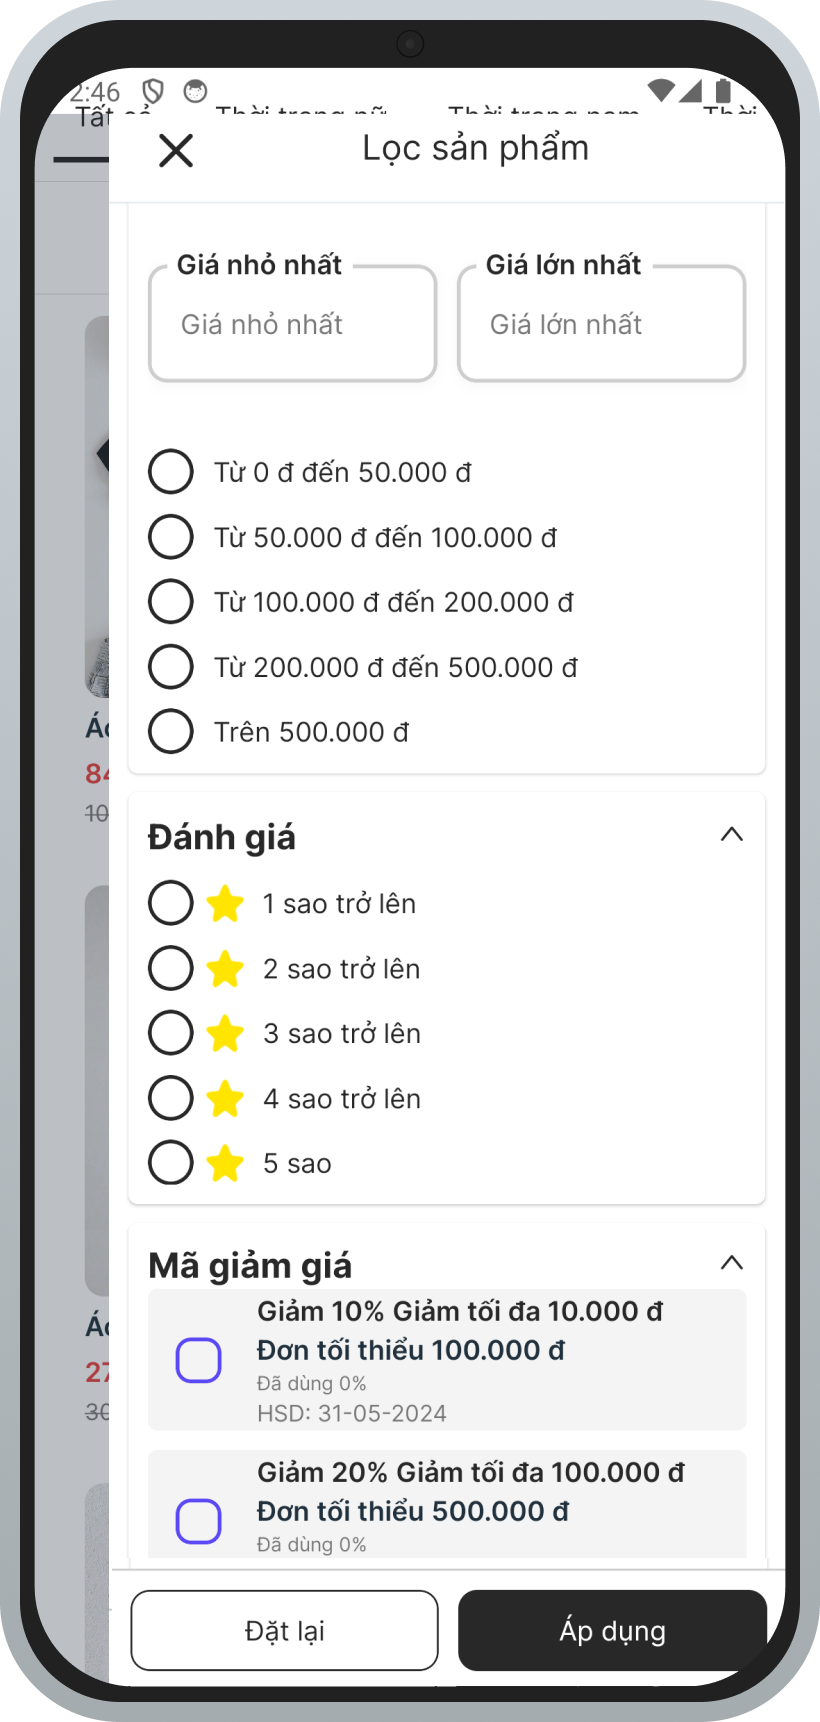
\includegraphics[width=5cm]{Images/Design/User/Main/Filter-1.png}
        \vspace{10pt}
        \centering \caption{Lọc sản phẩm}
    \end{minipage}
    \end{figure}

\newpage

\section{Kiểm thử hệ thống}
\subsection{Kiểm thử Web}
Môi trường kiểm thử:
\begin{enumerate}[-]
    \item Hệ điều hành: Windows
    \item Phiên bản hệ điều hành: 23H2 (OS Build 22631.3593)
    \item Phiên bản trình duyệt Chrome: 124.0.6367.208
\end{enumerate}
Đầu tiên là bảng Kiểm thử các yêu cầu chức năng của trang Dashboard, nơi hiển thị tổng số đơn hàng theo từng trạng thái, tổng giá trị đơn hàng theo từng trạng thái, doanh thu và các sản phẩm bán chạy.
\begin{longtable}{|p{4cm}|p{4cm}|p{4cm}|p{2cm}|}
    \hline
    Chức năng & Tiền điều kiện & Kết quả dự kiến & Kết quả \\
    \hline
    A1. Hiển thị tổng số đơn hàng theo từng trạng thái & Truy cập vào trang Dashboard & Hiển thị tổng số đơn hàng theo từng trạng thái & Đạt\\
    \hline
     A2. Hiển thị tổng giá trị đơn hàng theo từng trạng thái & Truy cập vào trang Dashboard & Hiển thị tổng giá trị đơn hàng theo từng trạng thái & Đạt\\
    \hline
     A3. Hiển thị doanh thu tháng này & Truy cập vào trang Dashboard, ở phần doanh thu có chế độ mặc định "Tháng này"  & Hiển thị doanh thu tháng này & Đạt\\
     \hline
     A4. Hiển thị doanh thu tháng trước & Truy cập vào trang Dashboard, ở phần doanh thu chọn chế độ "Tháng trước" & Hiển thị doanh thu tháng trước & Đạt \\
     \hline
     A5. Hiển thị doanh thu trong một khoảng thời gian & Truy cập vào trang Dashboard, ở phần doanh thu chọn chế độ "Tùy chỉnh khoảng thời gian" và chọn khoảng thời gian & Hiển thị doanh thu trong khoảng thời gian đã chọn & Đạt \\
     \hline
     A6. Hiển thị danh sách các sản phẩm bán chạy trong tháng này & Truy cập vào trang Dashboard, ở phần sản phẩm bán chạy có chế độ mặc định là "Tháng này" & Hiển thị danh sách các sản phẩm bán chạy trong tháng này & Đạt \\
     \hline 
     A7. Hiển thị danh sách các sản phẩm bán chạy trong tháng trước & Truy cập vào trang Dashboard, ở phần sản phẩm bán chạy chọn chế độ "Tháng này" & Hiển thị danh sách các sản phẩm bán chạy trong tháng này & Đạt \\
     \hline 
     A8. Hiển thị danh sách các sản phẩm bán chạy trong tuần này & Truy cập vào trang Dashboard, ở phần sản phẩm bán chạy chọn chế độ "Tuần này" & Hiển thị danh sách các sản phẩm bán chạy trong tuần này & Đạt \\
     \hline 
     A9. Hiển thị danh sách các sản phẩm bán chạy trong tuần trước & Truy cập vào trang Dashboard, ở phần sản phẩm bán chạy chọn chế độ "Tuần trước" & Hiển thị danh sách các sản phẩm bán chạy trong tuần trước & Đạt \\
    \hline
    \caption{Bảng kiểm thử yêu cầu chức năng trang Dashboard}
\end{longtable}
Tiếp theo là bảng Kiểm thử các yêu cầu chức năng của trang thể loại, bao gồm hiển thị các thể loại theo dạng cây thư mục, chức năng tạo, chỉnh sửa, xóa thể loại.
\begin{longtable}{|p{4cm}|p{4cm}|p{4cm}|p{2cm}|}
    \hline
    Chức năng & Tiền điều kiện & Kết quả dự kiến & Kết quả \\
    \hline
    B1. Hiển thị danh sách tất cả các thể loại& Truy cập vào trang thể loại & Hiển thị danh sách tất cả các thể loại theo dạng cây thư mục & Đạt\\
    \hline
     B2. Tạo mới thể loại & Nhấn vào button thêm thể loại và nhập các thông tin cho thể loại mới  & Hiển thị thể loại mới trong cây thư mục đúng vị trí & Đạt\\
    \hline
     B3. Cập nhật thể loại & Nhấn vào icon Edit và chỉnh sửa các thông tin của thể loại & Hiển thị lại danh sách thể loại theo đúng cấu trúc cây thư mục sau khi vừa cập nhật thể loại  & Đạt\\
    \hline
    B4. Xóa thể loại & Nhấn vào icon Delete và xác nhận có muốn xóa thể loại vừa nhấn hay không & Hiển thị lại danh sách thể loại theo đúng cấu trúc cây thư mục sau khi vừa xóa thể loại & Đạt\\
    \hline
    \caption{Bảng kiểm thử các yêu cầu chức năng của trang thể loại}
\end{longtable}
Tiếp theo là bảng Kiểm thử các yêu cầu chức năng của trang sản phẩm, nơi hiển thị danh sách tất cả các sản phẩm, hỗ trợ tính năng lọc/tìm kiếm các sản phẩm, hiển thị chi tiết các sản phẩm, tạo mới/cập nhật/ sản phẩm
\begin{longtable}{|p{4cm}|p{4cm}|p{4cm}|p{2cm}|}
    \hline
    Chức năng & Tiền điều kiện & Kết quả dự kiến & Kết quả \\
    \hline
    C1. Hiển thị danh sách tất cả các sản phẩm  & Truy cập vào trang sản phẩm & Hiển thị danh sách tất cả các sản phẩm & Đạt\\
    \hline
     C2. Hiển thị chi tiết sản phẩm  & Truy cập vào trang sản phẩm và nhấn xem chi tiết một sản phẩm & Hiển thị các thông tin chi tiết của sản phẩm & Đạt\\
    \hline
     C3. Tạo mới sản phẩm & Nhấn vào button thêm sản phẩm và nhập các thông tin cho sản phẩm mới & Tạo mới sản phẩm thành công và hiển thị form cho phép có thể thêm variant cho sản phẩm mới & Đạt\\
    \hline
    C4. Cập nhật sản phẩm & Nhấn button cập nhật ở trang chi tiết sản phẩm và chỉnh sửa các thông tin sản phẩm & Hiển thị lại thông tin sản phẩm sau khi đã cập nhật & Đạt\\
    \hline
    C5. Tìm kiếm sản phẩm & Nhập từ khóa vào ô tìm kiếm & Hiển thị các sản phẩm có tên chứa từ khóa đã nhập & Đạt \\
    \hline
    C6. Lọc sản phẩm theo min price và max price & Nhập phạm vi giá cả cho sản phẩm & Hiển thị các sản phẩm nằm trong phạm vi min price và max price & Đạt  \\
    \hline
    C7. Lọc sản phẩm theo số sao đánh giá sản phẩm & Chọn số sao đánh giá cho sản phẩm & Hiển thị các sản phẩm tương ứng với số sao đã chọn  & Đạt\\
    \hline
    C8. Lọc sản phẩm theo thể loại & Chọn thể loại muốn lọc & Hiển thị các sản phẩm tương ứng với thể loại đã chọn & Đạt \\
    \hline
    C9. Sắp xếp sản phẩm & Chọn chế độ muốn sắp xếp sản phẩm & Hiển thị các sản phẩm theo chế độ sắp xếp & Đạt\\
    \hline
    \caption{Bảng kiểm thử các yêu cầu chức năng của trang sản phẩm}
\end{longtable}
Tiếp theo là bảng Kiểm thử các yêu cầu chức năng của Review, bao gồm xem tất cả đánh giá của từng sản phẩm và xóa đánh giá sản phẩm.
\begin{longtable}{|p{4cm}|p{4cm}|p{4cm}|p{2cm}|}
    \hline
    Chức năng & Tiền điều kiện & Kết quả dự kiến & Kết quả \\
    \hline
    D1. Hiển thị tất cả các đánh giá của một sản phẩm  & Xem chi tiết một sản phẩm và chọn vào tab đánh giá sản phẩm & Hiển thị tất cả các đánh giá của sản phẩm đó & Đạt\\
    \hline
     D2. Xóa đánh giá sản phẩm  & Nhấn icon Delete tại đánh giá sản phẩm muốn xóa & Danh sách đánh giá sản phẩm được cập nhật lại sau khi vừa xóa đánh giá & Đạt\\
    \hline
    \caption{Bảng kiểm thử các yêu cầu chức năng của trang variant}
\end{longtable}
Tiếp theo là bảng Kiểm thử các yêu cầu chức năng của trang Variant, nơi hiển thị danh sách tất cả các variant theo từng sản phẩm, tạo mới/chỉnh sửa/cập nhật/xóa các variant.
\begin{longtable}{|p{4cm}|p{4cm}|p{4cm}|p{2cm}|}
    \hline
    Chức năng & Tiền điều kiện & Kết quả dự kiến & Kết quả \\
    \hline
    E1. Hiển thị danh sách các variant theo sản phẩm  & Truy cập vào trang sản phẩm và nhấn xem chi tiết một sản phẩm & Hiển thị danh sách variant theo sản phẩm dưới dạng bảng & Đạt\\
    \hline
     E2. Thêm variant cho sản phẩm & Nhấn button thêm variant và nhập các thông tin cho variant mới & Variant mới được hiển thị trong bảng variant của sản phẩm  & Đạt\\
    \hline
     E3. Cập nhật variant của sản phẩm& Nhấn icon Edit của variant muốn chỉnh sửa & Bảng variant cập nhật thông tin cho variant vừa được chỉnh sửa  & Đạt\\
     E4. Xóa variant của sản phẩm & Nhấn icon Delete của variant muốn xóa & Bảng variant không còn chứa variant vừa xóa & Đạt \\
    \hline
    \caption{Bảng kiểm thử các yêu cầu chức năng của trang variant}
\end{longtable}
Tiếp theo là bảng Kiểm thử các yêu cầu chức năng của trang mã giảm giá, nơi hiển thị danh sách tất cả các mã giảm giá, tạo mới/chỉnh sửa/cập nhật/xóa các mã giảm giá, gán mã giảm giá cho thể loại/sản phẩm/variant/người dùng.
\begin{longtable}{|p{4cm}|p{4cm}|p{4cm}|p{2cm}|}
    \hline
    Chức năng & Tiền điều kiện & Kết quả dự kiến & Kết quả \\
    \hline
    F1. Hiển thị danh sách tất cả mã giảm giá & Truy cập vào trang mã giảm giá & Hiển thị danh sách tất cả mã giảm giá dưới dạng bảng & Đạt\\
    \hline
     F2. Tạo mới mã giảm giá & Nhấn vào button thêm mã giảm giá trong trang mã giảm giá và nhập các thông tin cho mã giảm giá mới & Mã giảm giá mới được hiển thị trong bảng & Đạt\\
    \hline
     F3. Hiển thị thông tin chi tiết của mã giảm giá & Nhấn vào button Xem chi tiết của một mã giảm giá trong bảng  & Hiển thị thông tin chi tiết của mã giảm giá & Đạt\\
     \hline
     F4. Chỉnh sửa thông tin của mã giảm giá & Nhấn vào icon Edit của một mã giảm giá trong bảng và chỉnh sửa các thông tin & Hiển thị thông tin sau khi cập nhật của mã giảm giá trong bảng & Đạt\\
     \hline
     F5. Xóa mã giảm giá & Nhấn vào button Delete của một mã giảm giá & Mã giảm giá xóa thành công khỏi bảng & Đạt \\
     \hline
     F6. Cập nhật thể loại cho mã giảm giá & Nhấn vào button cập nhật thể loại và chọn thể loại tương ứng & Mã giảm giá đã cập nhật thể loại & Đạt\\
     \hline
     F7. Cập nhật người dùng cho mã giảm giá & Nhấn vào button Gán mã giảm giá cho người dùng và chọn các người dùng được áp dụng & Mã giảm giá đã được áp dụng cho các người dùng được chọn & Đạt \\
    \hline
    \caption{Bảng kiểm thử các yêu cầu chức năng của trang mã giảm giá}
\end{longtable}
Tiếp theo là bảng Kiểm thử các yêu cầu chức năng của trang đơn hàng, nơi hiển thị danh sách tất cả các đơn hàng theo trạng thái, xem chi tiết từng đơn hàng, cập nhật trạng thái đơn hàng.
\begin{longtable}{|p{4cm}|p{4cm}|p{4cm}|p{2cm}|}
    \hline
    Chức năng & Tiền điều kiện & Kết quả dự kiến & Kết quả \\
    \hline
    G1. Hiển thị danh sách tất cả các đơn hàng & Truy cập vào trang đơn hàng & Hiển thị danh sách tất cả các đơn hàng theo trạng thái & Đạt\\
    \hline
     G2. Hiển thị thông tin chi tiết của đơn hàng & Truy cập vào trang đơn hàng và nhấn button Xem chi tiết vào một đơn hàng & Hiển thị thông tin chi tiết đơn hàng đó & Đạt\\
    \hline
     G3. Hiển thị các sản phẩm trong đơn hàng & Truy cập vào trang đơn hàng và nhấn button Xem chi tiết vào một đơn hàng  & Hiển thị các sản phẩm trong đơn hàng & Đạt\\
     \hline
     G4. Hiển thị giá trị của đơn hàng & Truy cập vào trang đơn hàng và nhấn button Xem chi tiết vào một đơn hàng  & Hiển thị giá trị của đơn hàng & Đạt\\
      \hline
     G5. Cập nhật trạng thái của đơn hàng & Truy cập vào trang đơn hàng và nhấn button Xem chi tiết vào một đơn hàng, chọn trạng thái phù hợp để cập nhật  & Cập nhật trạng thái của đơn hàng & Đạt\\
    \hline
    \caption{Bảng kiểm thử các yêu cầu chức năng của trang đơn hàng}
\end{longtable}
Tiếp theo là bảng Kiểm thử các yêu cầu chức năng của trang khách hàng, nơi hiển thị danh sách tất cả các khách hàng, xem thông tin cá nhân, thông tin nhận hàng, các đơn hàng đã đặt, các đánh giá sản phẩm của từng khách hàng.
\begin{longtable}{|p{4cm}|p{4cm}|p{4cm}|p{2cm}|}
    \hline
    Chức năng & Tiền điều kiện & Kết quả dự kiến & Kết quả \\
    \hline
    H1. Hiển thị danh sách tất cả các khách hàng & Truy cập vào trang khách hàng & Hiển thị danh sách tất cả các khách hàng & Đạt\\
    \hline
     H2. Hiển thị thông tin cá nhân của khách hàng & Nhấn vào button Xem chi tiết của một khách hàng trong bảng & Hiển thị thông tin cá nhân của một khách hàng & Đạt\\
    \hline
     H3. Hiển thị thông tin nhận hàng của khách hàng & Chuyển qua tab "Thông tin nhận hàng" của trang xem thông tin cá nhân của khách hàng & Hiển thị thông tin nhận hàng của khách hàng & Đạt\\
     \hline
     H4. Hiển thị các đơn hàng của một khách hàng & Chuyển qua tab "Thông tin nhận hàng" của trang xem thông tin cá nhân của khách hàng & Hiển thị các đơn hàng của khách hàng & Đạt\\
     \hline
      H5. Hiển thị các đánh giá sản phẩm của một khách hàng & Chuyển qua tab "Đánh giá sản phẩm" của trang xem thông tin cá nhân của khách hàng & Hiển thị các đánh giá sản phẩm của khách hàng & Đạt\\
    \hline
    \caption{Bảng kiểm thử các yêu cầu chức năng của trang khách hàng}
\end{longtable}
Tiếp theo là bảng Kiểm thử các yêu cầu chức năng của trang nhân viên, nơi hiển thị danh sách tất cả các nhân viên, xem thông tin cá nhân của từng nhân viên.
\begin{longtable}{|p{4cm}|p{4cm}|p{4cm}|p{2cm}|}
    \hline
    Chức năng & Tiền điều kiện & Kết quả dự kiến & Kết quả \\
    \hline
    I1. Hiển thị danh sách tất cả các nhân viên & Truy cập vào trang nhân viên & Hiển thị danh sách tất cả các nhân viên & Đạt\\
    \hline
     I2. Hiển thị thông tin chi tiết của một nhân viên & Nhấn vào button Xem chi tiết của một nhân viên trong bảng  & Hiển thị thông tin chi tiết của nhân viên & Đạt\\
    \hline
    \caption{Bảng kiểm thử các yêu cầu chức năng của trang nhân viên}
\end{longtable}
\newpage
\subsection{Kiểm thử Ứng dụng di động}
Môi trường kiểm thử:
\begin{enumerate}[-]
    \item Hệ điều hành: Android
    \item Phiên bản hệ điều hành: Android 14
\end{enumerate}
\noindent Chức năng đăng nhập/đăng ký
\begin{longtable}{|p{4cm}|p{4cm}|p{4cm}|p{2cm}|}
    \hline
    Chức năng & Tiền điều kiện & Kết quả dự kiến & Kết quả \\
    \hline
    A1. Đăng nhập bằng tài khoản, mật khẩu đúng & Nhập tên đăng nhập và mật khẩu & Hiển thị thông báo đăng nhập thành công, chuyển đến trang chủ & Đạt\\
    \hline
    A2. Đăng nhập bằng tài khoản không hợp lệ & Nhập tên đăng nhập và mật khẩu không hợp lệ & Hiển thị thông báo không tìm thấy tài khoản & Đạt\\
    \hline
    A3. Đăng nhập bỏ trống tài khoản & Nhập mật khẩu & Vô hiệu hoá nút Đăng nhập & Đạt\\
    \hline
    A4. Đăng nhập bỏ trống mật khẩu & Nhập tài khoản & Vô hiệu hoá nút Đăng nhập & Đạt\\
    \hline
    A5. Đăng nhập bằng tài khoản đúng nhưng mật khẩu sai & Nhập tài khoản, và mật khẩu không đúng & Hiển thị thông báo nhập sai mật khẩu & Đạt\\
    \hline
    A6. Đăng nhập bằng Google & Chọn tuỳ chọn đăng nhập bàng Google & Hiển thị thông báo đăng nhập thành công với tài khoản Google & Đạt\\
    \hline
     A7. Đăng ký bằng tài khoản, mật khẩu & Nhập mật khẩu, số điện thoại và email chưa được sử dụng & Hiển thị thông báo đăng ký thành công & Đạt\\
    \hline
    A8. Đăng ký bằng số điện thoại đã tồn tại & Nhập mật khẩu, số điện thoại đã tồn tại và email chưa được sử dụng & Hiển thị thông báo số điện thoại đã được đăng ký & Đạt\\
    \hline
    A9. Đăng ký bằng email đã tồn tại & Nhập mật khẩu, số điện thoại chưa sử dụng và email đã tồn tại & Hiển thị thông báo email đã được đăng ký & Đạt\\
    \hline
    A10. Đăng ký bằng email và số điện thoại đã tồn tại & Nhập mật khẩu, số điện thoại chưa sử dụng và email đã tồn tại & Hiển thị thông báo email đã được đăng ký & Đạt\\
    \hline
    A11. Đăng ký bằng tài khoản, mật khẩu bỏ trống các trường thông tin & Không nhập một số trường thông tin & Vô hiệu hoá nút đăng ký & Đạt\\
    \hline
    \caption{Kiểm thử yêu cầu chức năng trang đăng nhập và đăng ký}
\end{longtable}

\noindent Chức năng tìm kiếm, lọc sản phẩm, nơi người dùng có thể tìm kiếm sản phẩm theo tên, hình ảnh, sắp xếp sản phẩm. Người dùng cần phải bấm vào ô tìm kiếm hoặc icon hình camera bên cạnh ô tìm kiếm để thực hiện chức năng.

\begin{longtable}{|p{4cm}|p{4cm}|p{4cm}|p{2cm}|}
    \hline
    Chức năng & Tiền điều kiện & Kết quả dự kiến & Kết quả \\
    \hline
    B1. Tìm kiếm sản phẩm theo tên có tồn tại & Nhập tên một sản phẩm tồn tại  & Hiển thị đúng sản phẩm theo tên & Đạt\\
    \hline
    B2. Tìm kiếm sản phẩm bằng hình ảnh & Nhấn vào biểu tượng Camera, tài lên 1 hình ảnh & Hiển thị những sản phẩm được tìm thấy bằng hình ảnh & Đạt\\
    \hline
    B3. Tìm kiếm sản phẩm theo danh mục & Dưới thanh tìm kiếm hiển thị một số danh mục, và chọn vào 1 danh mục & Hiển thị những sản phẩm theo danh mục đã chọn & Đạt\\
    \hline
    B4. Sắp xếp những sản phẩm theo giá & Chọn vào mục Sắp xếp, sau đó chọn giắ tăng dần hoặc giảm dần & Hiển thị những sản phẩm được sắp xếp theo giá tăng dần hoặc giảm dần & Đạt\\
    \hline
    B5. Sắp xếp những sản phẩm theo phổ biến & Chọn vào mục Sắp xếp, sau đó phổ biến nhất & Hiển thị những sản phẩm được sắp xếp theo độ phổ biến & Đạt\\
    \hline
    B6. Sắp xếp những sản phẩm mới nhất & Chọn vào mục Sắp xếp, sau đó chọn Mới nhất & Hiển thị những sản phẩm được sắp xếp theo mới nhất & Đạt\\
    \hline
     B7. Sắp xếp những sản phẩm được giảm giá nhiều nhất & Chọn vào mục Sắp xếp, sau đó chọn Giảm giá nhiều nhất & Hiển thị những sản phẩm được sắp xếp theo mức giảm giá nhiều nhất & Đạt\\
    \hline
    B8. Lọc sản phẩm theo giá tiền & Điền giá tiền nhỏ nhất và lớn nhất & Hiển thị những sản phẩm nằm trong giá tiền & Đạt\\
    \hline
    B9. Lọc sản phẩm theo số sao đánh giá & Chọn mức sao sản phẩm & Hiển thị những sản phẩm có số sao lớn hơn hoặc bằng mức đã chọn & Đạt\\
    \hline
    B10. Lọc sản phẩm theo mã giảm giá hiện có & Chọn mã voucher cần lọc & Hiển thị những sản phẩm có thể áp dụng được voucher & Đạt\\
    \hline
    \caption{Kiểm thử yêu cầu chức năng tìm kiếm sản phẩm}
\end{longtable}

\noindent Chức năng quản lý giỏ hàng, bao gồm việc thêm sản phẩm vào giỏ hàng hoặc xoá, để có thể thêm sản phẩm vào được giỏ hàng thì bắt buộc người dùng phải đăng nhập trước.

\begin{longtable}{|p{4cm}|p{4cm}|p{4cm}|p{2cm}|}
    \hline
    Chức năng & Tiền điều kiện & Kết quả dự kiến & Kết quả \\
    \hline
    C1. Thêm một sản phẩm vào giỏ hàng đã chọn kích thước, màu sắc  & Chọn kích thước, màu sắc và chọn thêm vào giỏ & Hiển thị thông báo Thêm vào giỏ hàng thành công  & Đạt\\
    \hline
    C2. Thêm một sản phẩm vào giỏ hàng mà không chọn kích thước hoặc màu sắc & Không chọn kích thước hoặc màu sắc & Vô hiệu hoá nút thêm vào giỏ hàng & Đạt\\
    \hline
    C3. Thêm một sản phẩm mà số lượng đã hết & Chọn vào sản phẩm có số lượng là 0 & Vô hiệu hoá việc chọn sản phẩm có số lượng bằng 0 và Thêm vào giỏ & Đạt\\
    \hline
    C4. Thêm sản phẩm vào giỏ hàng mà chưa đăng nhập & Chọn sản phẩm, kích thước và màu sắc, sau đó chọn thêm vào giỏ hàng & Hiển thị thông báo yêu cầu đăng nhập & Đạt \\
    \hline
    C5. Xoá sản phẩm ra khỏi giỏ hàng & Ở trang giỏ hàng, người dùng bấm xoá sản phẩm & Sản phẩm được xoá khỏi giỏ hàng  & Đạt \\
    \hline
    C6. Xem sản phẩm có trong giỏ hàng & Chọn vào giỏ hàng & Hiển thị những sản phảm trong giỏ hàng & Đạt \\
    \hline
    C7. Mua hàng mà không chọn sản phẩm nào trong giỏ hàng & Bỏ chọn tất cả sản phẩm trong giỏ hàng & Vô hiệu hoá nút mua hàng & Đạt \\
    \hline
    C8. Mua hàng mà đã chọn một trong những sản phẩm trong giỏ hàng & Chọn sản phẩm trong giỏ hàng và bấm mua hàng & Chuyển đến trang đơn hàng & Đạt \\
    \hline
    \caption{Kiểm thử yêu cầu chức năng giỏ hàng}
\end{longtable}

\noindent Chức năng về sản phẩm yêu thích. Nơi sẽ lưu những sản phầm mà người dùng mong muốn sẽ mua trong tương lai.
\begin{longtable}{|p{4cm}|p{4cm}|p{4cm}|p{2cm}|}
    \hline
    Chức năng & Tiền điều kiện & Kết quả dự kiến & Kết quả \\
    \hline
    D1. Xem sản phẩm yêu thích & Chọn vào trang yêu thích & Hiên thị những sản phẩm đã đánh dấu yêu thích & Đạt \\
    \hline
    D2. Lọc sản phẩm theo danh mục & Ở trang yêu thích, chọn lọc theo danh mục & Sản phẩm yêu thích được lọc theo danh mục. & Đạt \\
    \hline
    D3. Thêm sản phẩm yêu thích & Bấm vào icon trái tim  & Hiện thông báo sản phẩm đã được thêm vào yêu thích & Đạt \\
    \hline
    D4. Xoá sản phẩm khỏi yêu thích & Bấm vào icon trái tim & Hiện thông bảo sản phẩm đã đượpc xoá khỏi yêu thích & Đạt \\
    \hline
    \caption{Kiểm thử yêu cầu chức năng sản phẩm yêu thích}
\end{longtable}



\newpage
%%%%%%%%%%%%%%%%%%%%%%%%%%%%%%%%%%%%%%%%%%%
\subsection{Kiểm thử API Backend}


\noindent Postman là một công cụ kiểm thử API được nhiều người ưa chuộng vì tính đa năng và dễ sử dụng. Sau khi triển khai server, chúng tôi đã tiến hành kiểm thử lên server có cấu hình như sau:
\begin{itemize}
    \item 1 CPU core
    \item 2 GB memory
    \item 25 GB SSD
    \item 1000 GB transfer
\end{itemize}
Tiếp tục, chúng tôi sử dụng performance test của postman để test các collection. Với cấu hình performance test như sau:
\begin{itemize}
    \item Virtual users: 100
    \item Test duration: 5 mins
    \item Load profile: Fixed
\end{itemize}
Kết quả chạy của các phiên như sau:

\begin{table}[H]
\centering
\begin{tabularx}{\textwidth}{|>{\centering\arraybackslash}X|>{\centering\arraybackslash}X|>{\centering\arraybackslash}X|>{\centering\arraybackslash}X|>{\centering\arraybackslash}X|}
\hline
Collection & Thời gian chạy & Tổng số request & Request/s & Thời gian phản hồi trung bình (ms) \\
\hline
User & 5 phút & 14.799 & 48.02 & 378 \\
\hline
Staff & 5 phút & 12.113 & 39.2 & 333 \\
\hline
Voucher & 5 phút & 7.442 & 24.19 & 341 \\
\hline
Review & 5 phút & 10.992 & 37.72 & 361 \\
\hline
Product & 5 phút & 15.235 & 53.25 & 427 \\
\hline
Order & 5 phút & 8.274 & 31.2 & 391 \\
\hline
Category & 5 phút & 12.643 & 35.19 & 301 \\
\hline
\end{tabularx}
\caption{Bảng số liệu hiệu năng Collection API}
\end{table}



\newpage

\section{Triển khai và đánh giá hệ thống}
\subsection{Triển khai hệ thống}
\subsubsection{Triển khai Web Service}
Hệ thống chúng tôi được triển khai như sau:
\begin{enumerate}[-]
    \item Deploy Server: Sử dụng Google Cloud để triển khai Web serivce với cấu hình 
    \item Cơ sở dữ liệu PosgreSQL: Sử dụng Aiven.io để triển khai cơ sở dữ liệu PosgreSQL, với cấu hình 1GB RAM / 1 Core CPU / 5Gb Storage.
    \item Cơ sở dữ liệu Neo4j: Sử dụng  neo4j Aura để triển khai cơ sở dữ liệu đồ thị với cấu hình 1GB RAM / 1 Core CPU / 5Gb Storage.
    \item Lưu trữ: Sử dụng service S3 của AWS để triển khai cho việc lưu trữ hình ảnh.
\end{enumerate}
Các bước triển khai hệ thống:

\begin{enumerate}[1.]
    \item \textbf{Chuẩn bị sẵn các dịch vụ sử dụng}: Ta cần tạo 1 máy ảo từ Google Cloud chạy hệ điều hành Linux và 1 database PosgreSQl từ Aiven và 1 cở sở dữ liệu Neo4j từ Aura.
    \item \textbf{Thiết lập khoá trên máy ảo}: Để có thể cấp quyền Pull code trên máy ảo, ta cần tạo khoá công khai và thêm vào tài khoản Git.
    \item \textbf{Tải và cập nhật các thư viện:} Chúng ta cần cập nhập thư viện có trong máy ảo và cài nginx, node, pm2 bằng các câu lệnh sau:\cite{deploy}
     \begin{enumerate}[-]
        \item sudo apt-get update
        \item sudo apt-get install nginx
        \item sudo systemctl start nginx
        \item sudo apt-get install nodejs
        \item sudo npm install pm2 -g
     \end{enumerate}
    \item \textbf{Thiết lập mã nguồn}: Sau khi Pull code về tạo ra file .env và bỏ tất cả các biến môi trường vào file này. Sau đó thực hiện lệnh build. Sau đó ta khởi chạy dự án với pm2 và kiếm tra trạng thái
    \begin{enumerate}[-]
        \item pm2 start dist/index.js
        \item pm2 status
    \end{enumerate}
    \item \textbf{Thiết lập nginx:} Thiết lập nginx cho các yêu cầu tới Nodejs. Ta mở tệp cấu hình nginx và cấu hình lại, proxy\_pass ta cần điền port mà ứng dụng chạy.
    \begin{enumerate}[-]
        \item sudo nano /etc/nginx/sites-available/default
        \item  \begin{figure}[H]
        \centering
        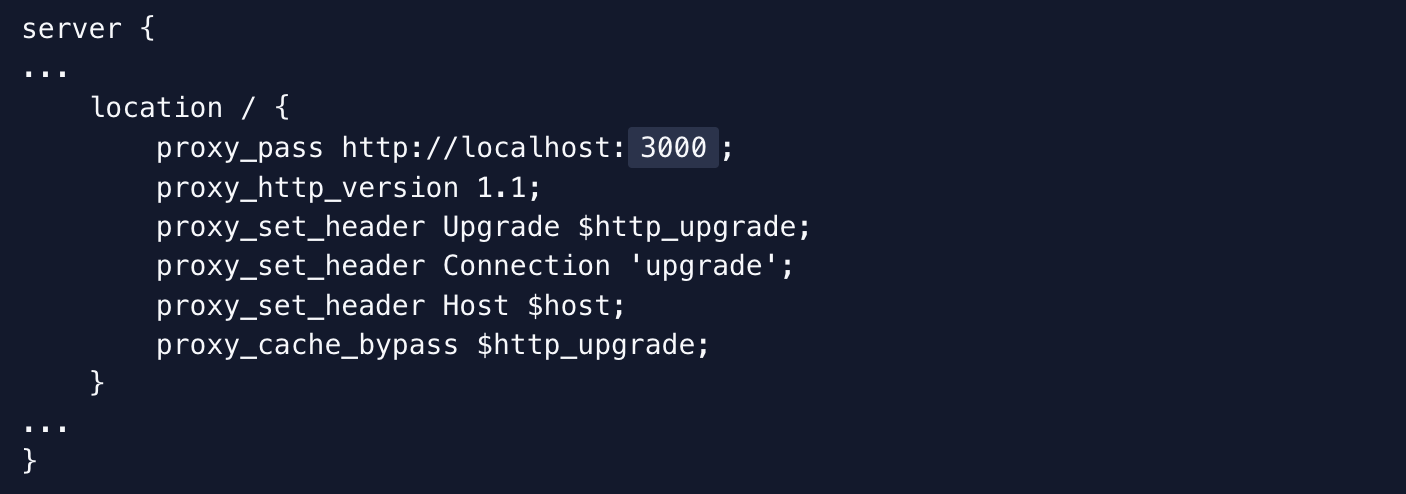
\includegraphics[width=10cm]{Images/Trienkhai/BE/nginxConfig.png}
        \newline
        \caption{Cấu hình nginx}
    \end{figure}
    \end{enumerate}
    \item \textbf{Kết quả: } Kiểm thử và khởi chạy lại nginx và ứng dụng đã được deploy thành công
    \begin{enumerate}[-]
        \item sudo systemctl restart nginx
    \end{enumerate}
\end{enumerate}
\subsubsection{Triển khai Website Admin trên Cloudflare}
Nhóm sử dụng dịch vụ của CloudFlare để triển khai trang web cho admin quản lý và mua tên miền từ id.tenten.vn. Các bước được thực hiện như sau:
\begin{enumerate}[1.]
    \item \textbf{Đăng ký tài khoản CloudFlare:} Đầu tiên chúng ta cần vào trang web của CloudFlare và tạo tài khoản nếu chưa có. Sau đó thực hiện đăng nhập.
    
    \item \textbf{Khởi tạo dự án:} Ở trang Dashboard, ở thanh sidebar chọn "Workers \& Pages" rồi chọn "Overview". Nội dung trang hiện ra ta chọn tiếp nút "Create Application"
    \begin{figure}[H]
        \centering
        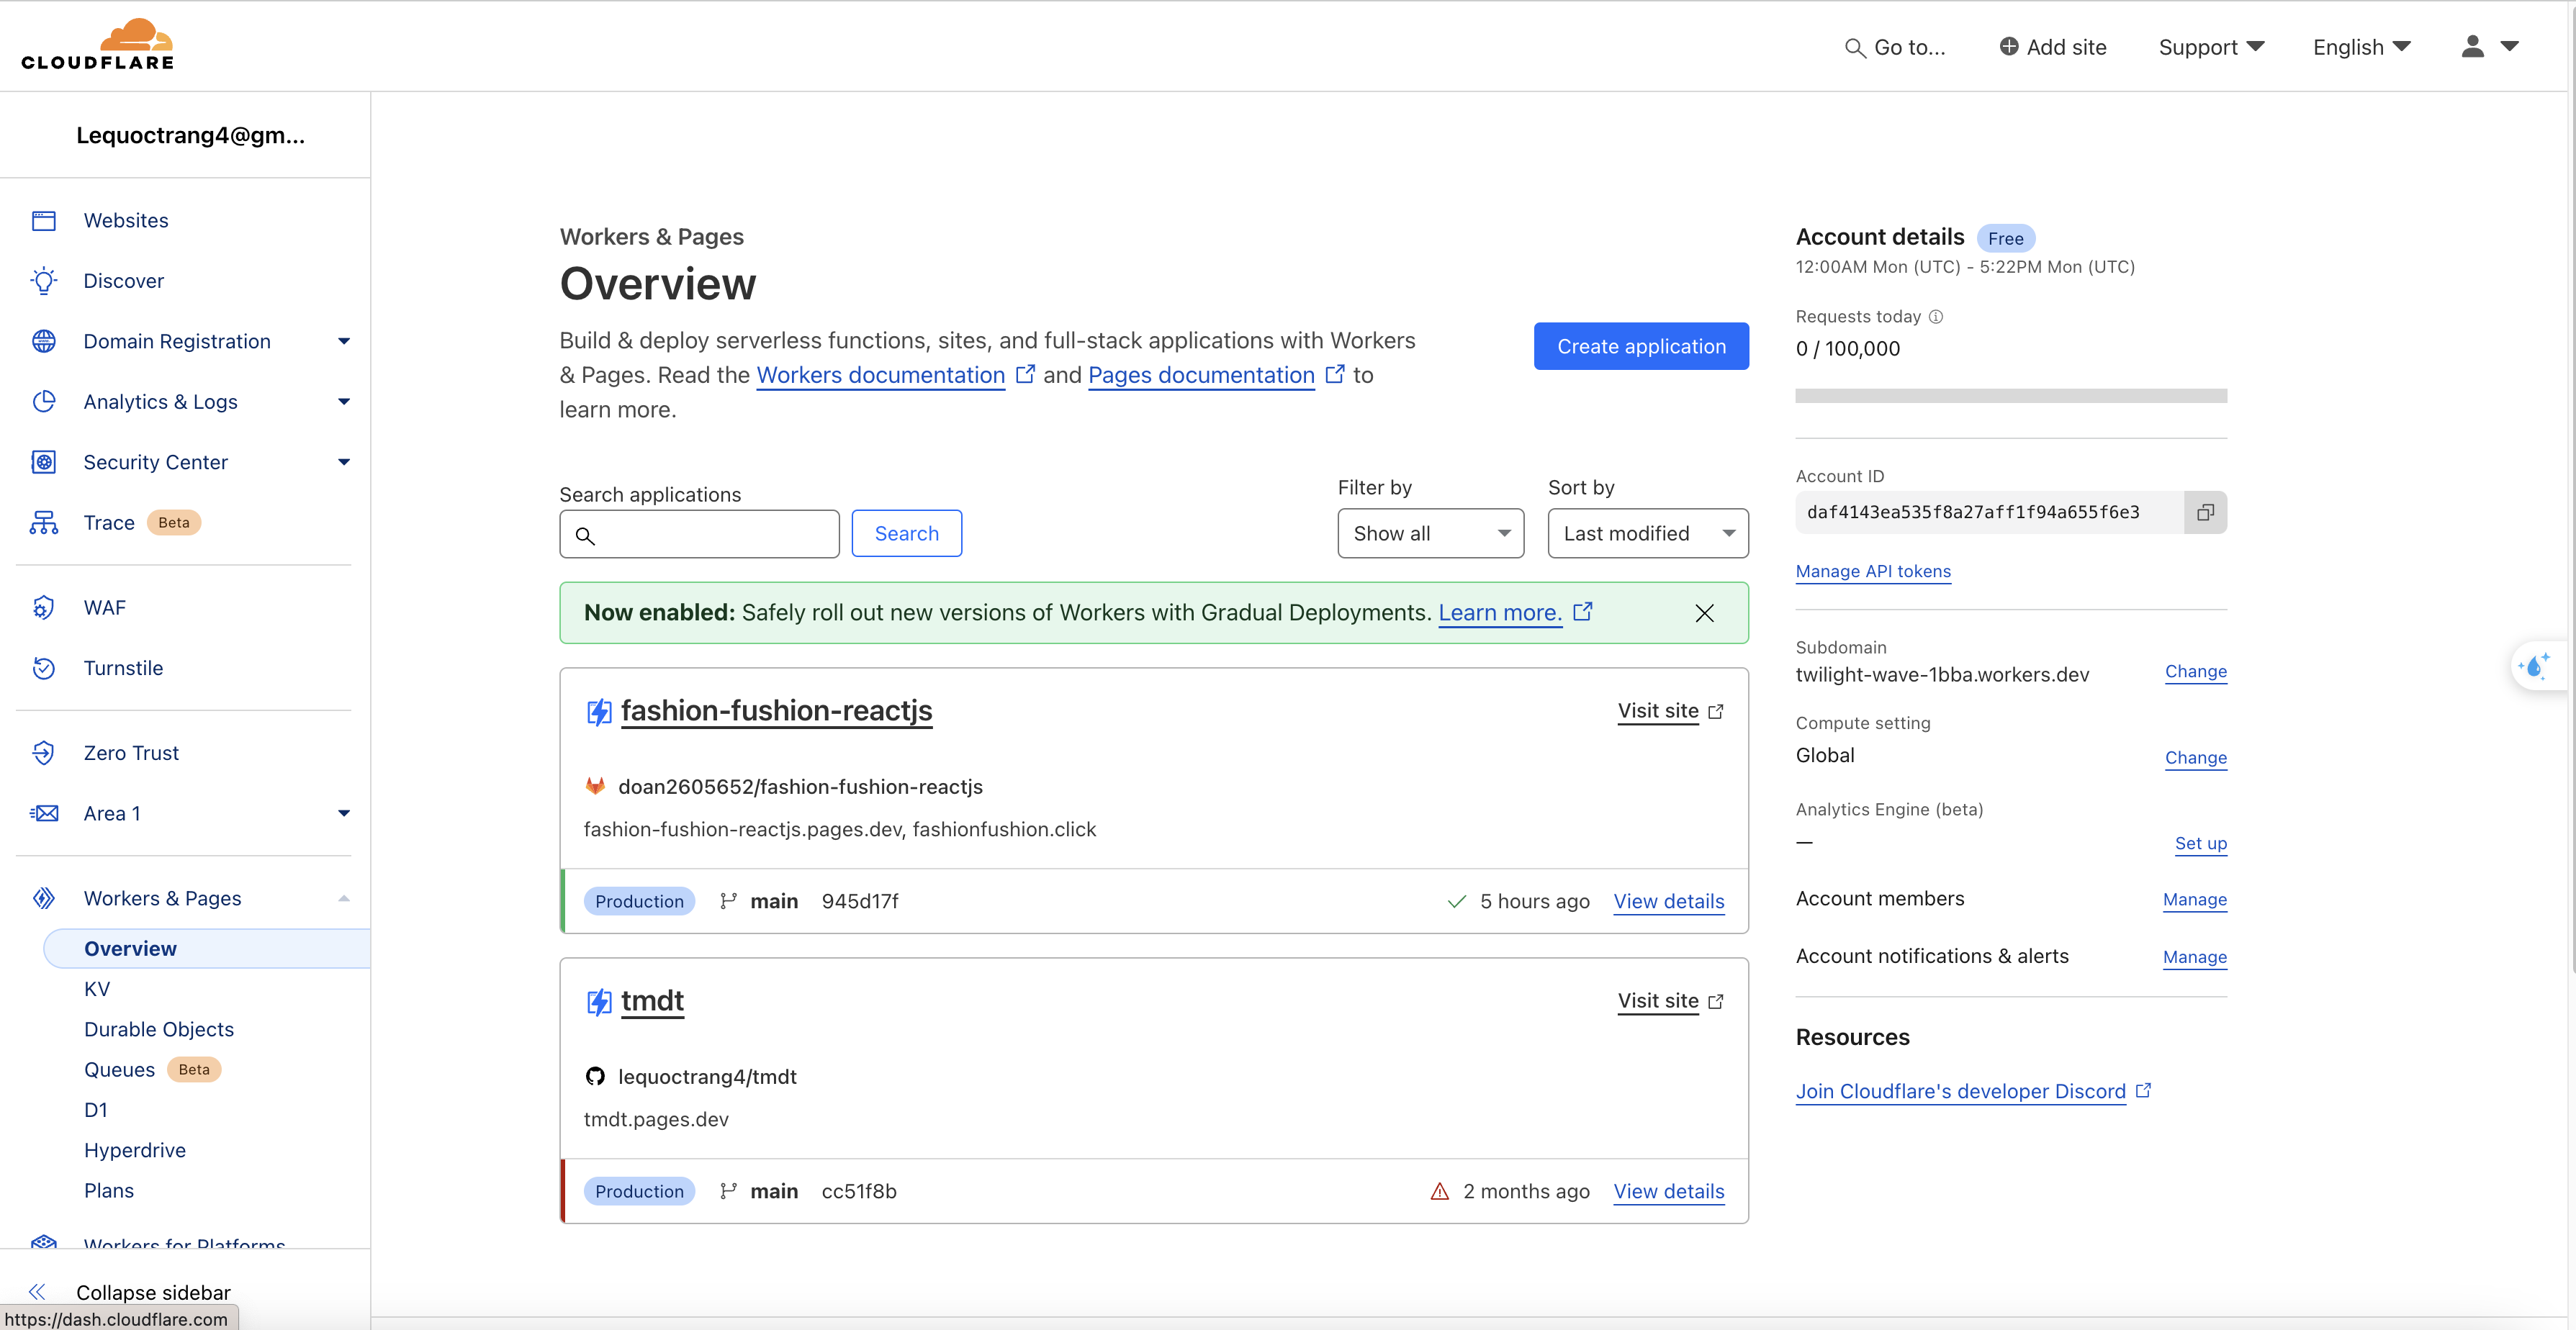
\includegraphics[width=16cm]{Images/Trienkhai/Web/step2.png}
        \newline
        \caption{Khởi tạo dự án trên CloudFlare}
    \end{figure}
    \item \textbf{Liên kết đến Git}: Sau đó chọn Mục "Page" và chọn "Connect To Git". Sau đó ta chọn dự án cần triển khai và chọn "Begin setup"
    \item  \textbf{Cấu hình dự án:} Sau khi tạo dự án, ta cần cấu hình dự án của mình. Đầu tiên cần chọn nhánh deploy là nhánh main. Sau đó ở phần "Framework preset" ta chọn "Create React App" thì CloudFlare sẽ tự xác định thư mục build và câu lệnh run build. Nếu chúng ta có sử dụng những câu lệnh build khác hay là chỉnh "Build output directory" thì cần phải sửa lại cho đúng. Tiếp theo là "Root Directory" và thiết lập các biến môi trường ở phần "Environment variables". Cuối cùng bấm "Save \& Deploy".
     \begin{figure}[H]
        \centering
        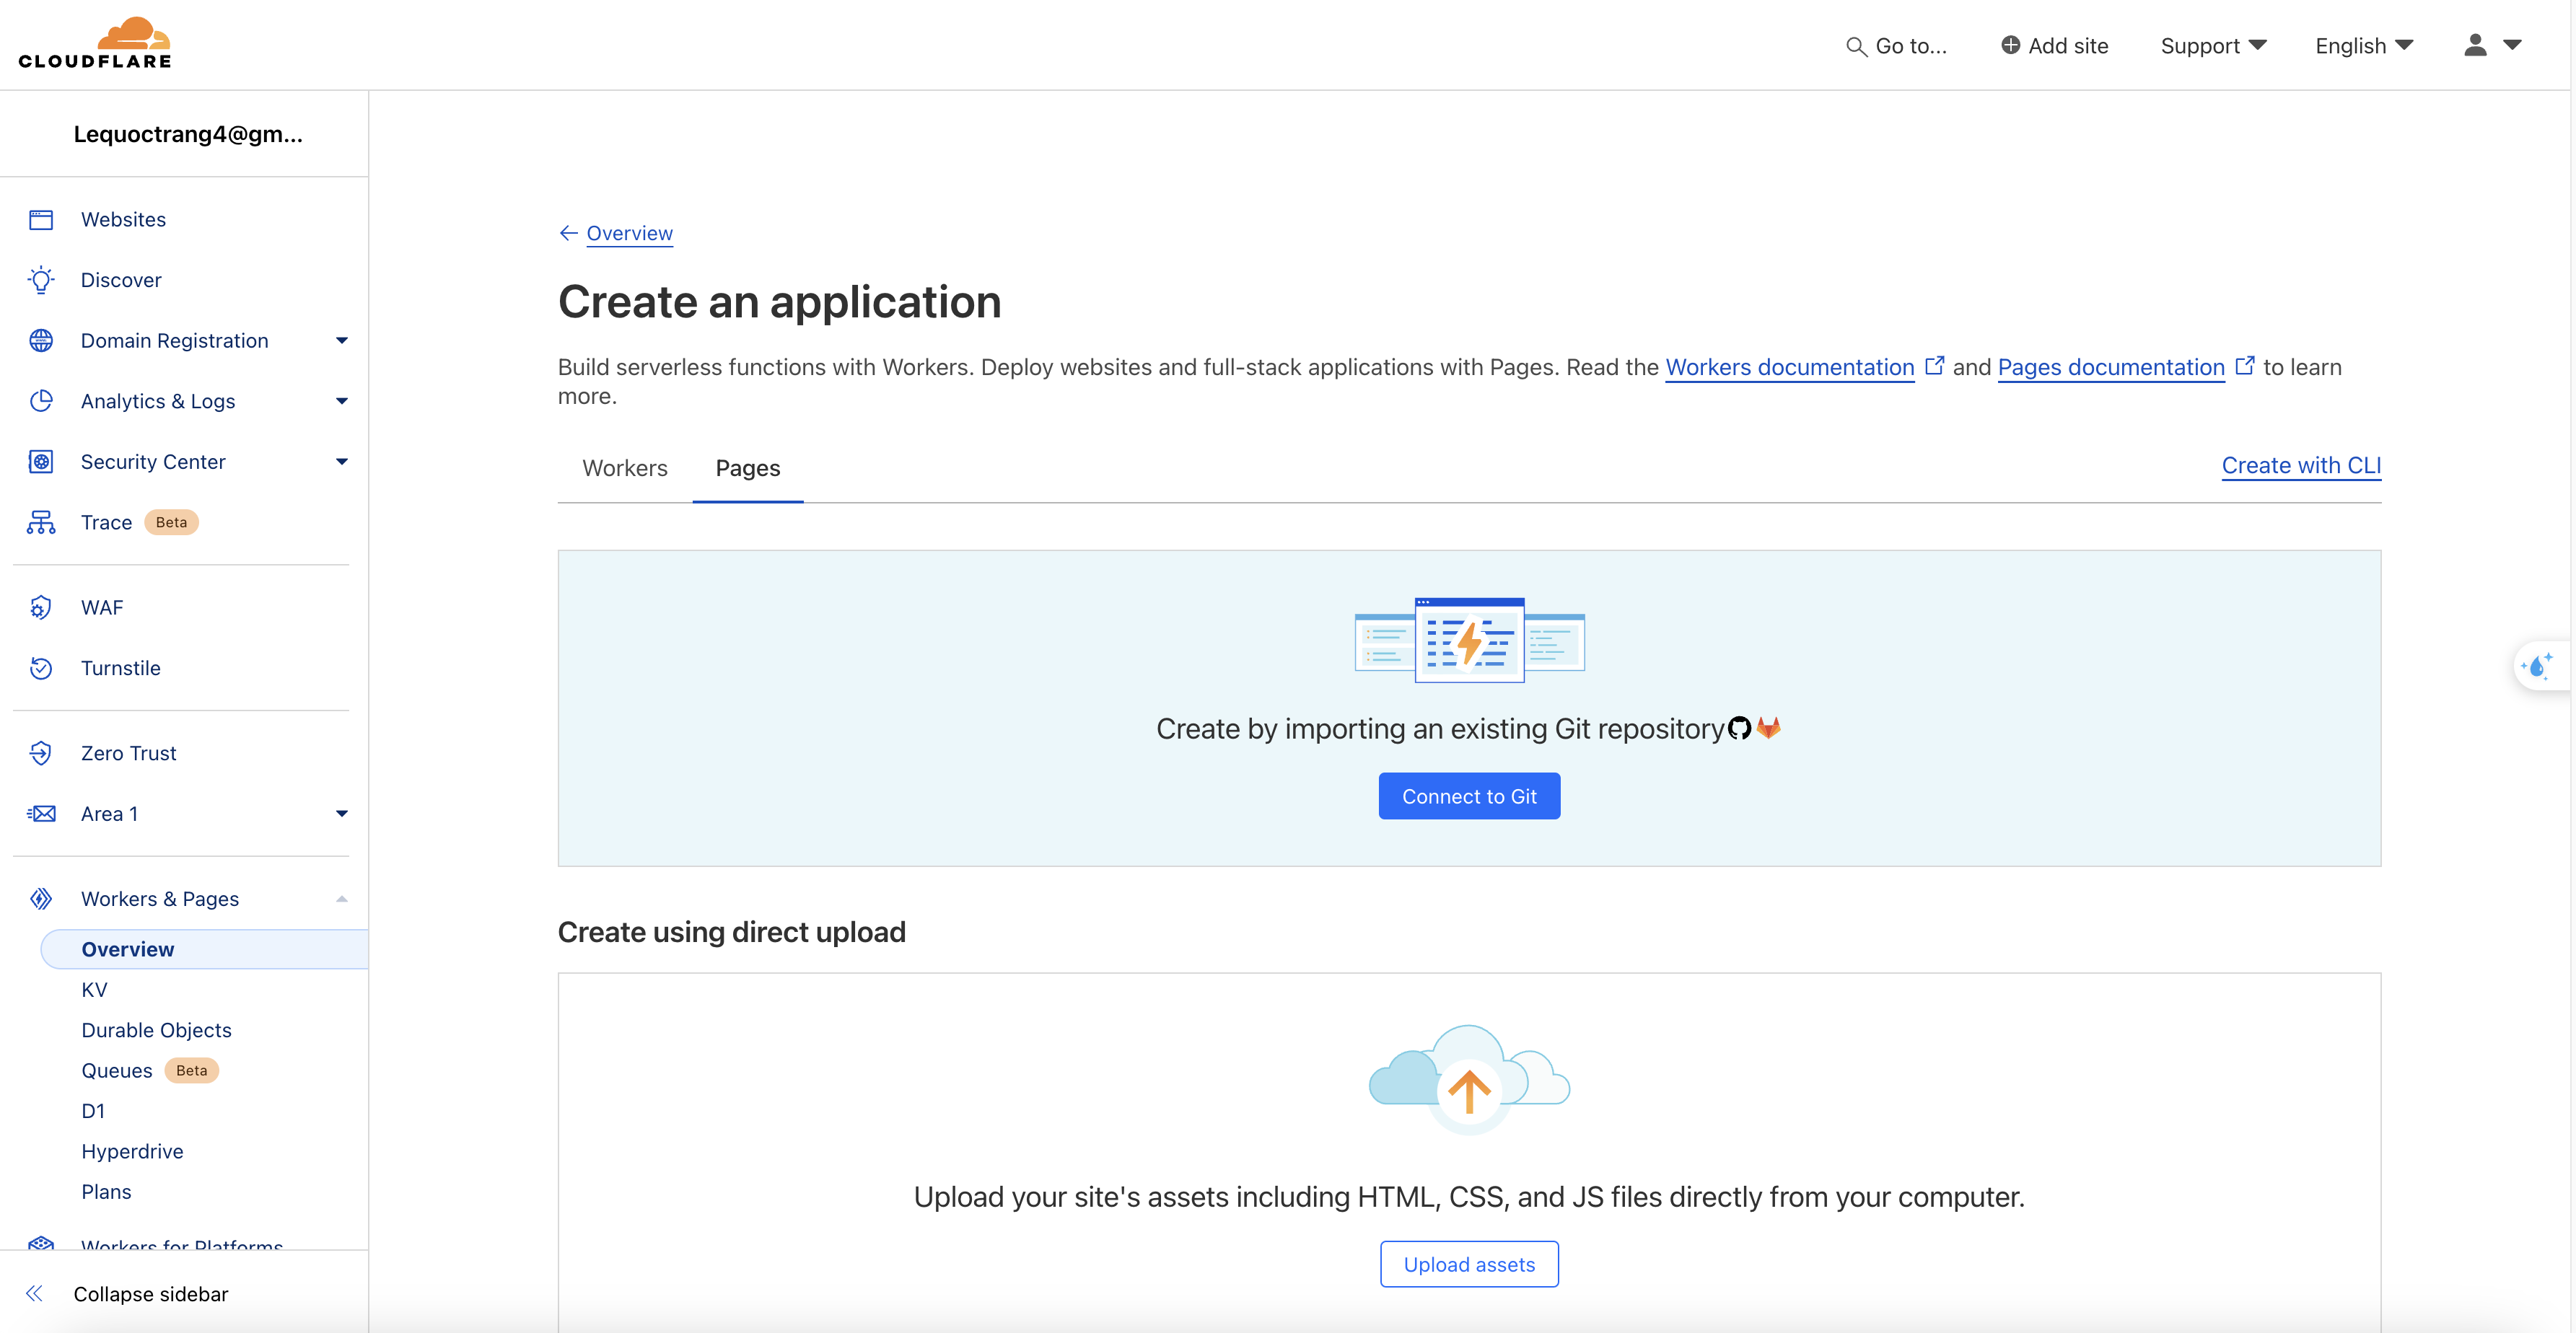
\includegraphics[width=16cm]{Images/Trienkhai/Web/step4.png}
        \newline
        \caption{Thiết lập các biến môi trường và tiến hành Deploy}
    \end{figure}
    
    \item \textbf{Xem kết quả:}  Sau khi triển khai thành công, CloudFlare sẽ cung cấp URL có thể sử dụng để xem ứng dụng đã triển khai.
\end{enumerate}
\subsubsection{Triển khai tên miền}
Sau khi mua được tên miền thì chúng tôi sẽ gắn tên miền đến địa chỉ IP của hệ thống và trang web. Ở đây chúng tôi sử dụng CloudFlare để thực hiện quản lý tên miền. Các bước được thực hiện như sau:

\begin{enumerate}[1.]
    \item \textbf{Xác thực tên miền: } Sau khi đăng nhập vào CloudFlare, ở mục thanh bên trái, chọn "Websites" rồi chọn "Add a site", sau đó điền tên miền đã chuẩn bị và thực hiện xác thực. Để thực hiện việc xác thực tên miền, ta cần thêm đường dẫn của Cloudflare cung cấp để thêm vào name server của tên miền.
    \item  \textbf{Thiết lập DNS: } Ở trang quản lý tên miền, ta chọn "DNS" -> "Record" ở thanh điều hướng bên trái. Sau đó bấm "Add record". Đối với Server thì ta cần chọn type là "A" vì cần nhập địa chỉ IPv4 còn đối với trang web thì ta chọn "CNAME"
\end{enumerate}
\begin{figure}[H]
    \centering
    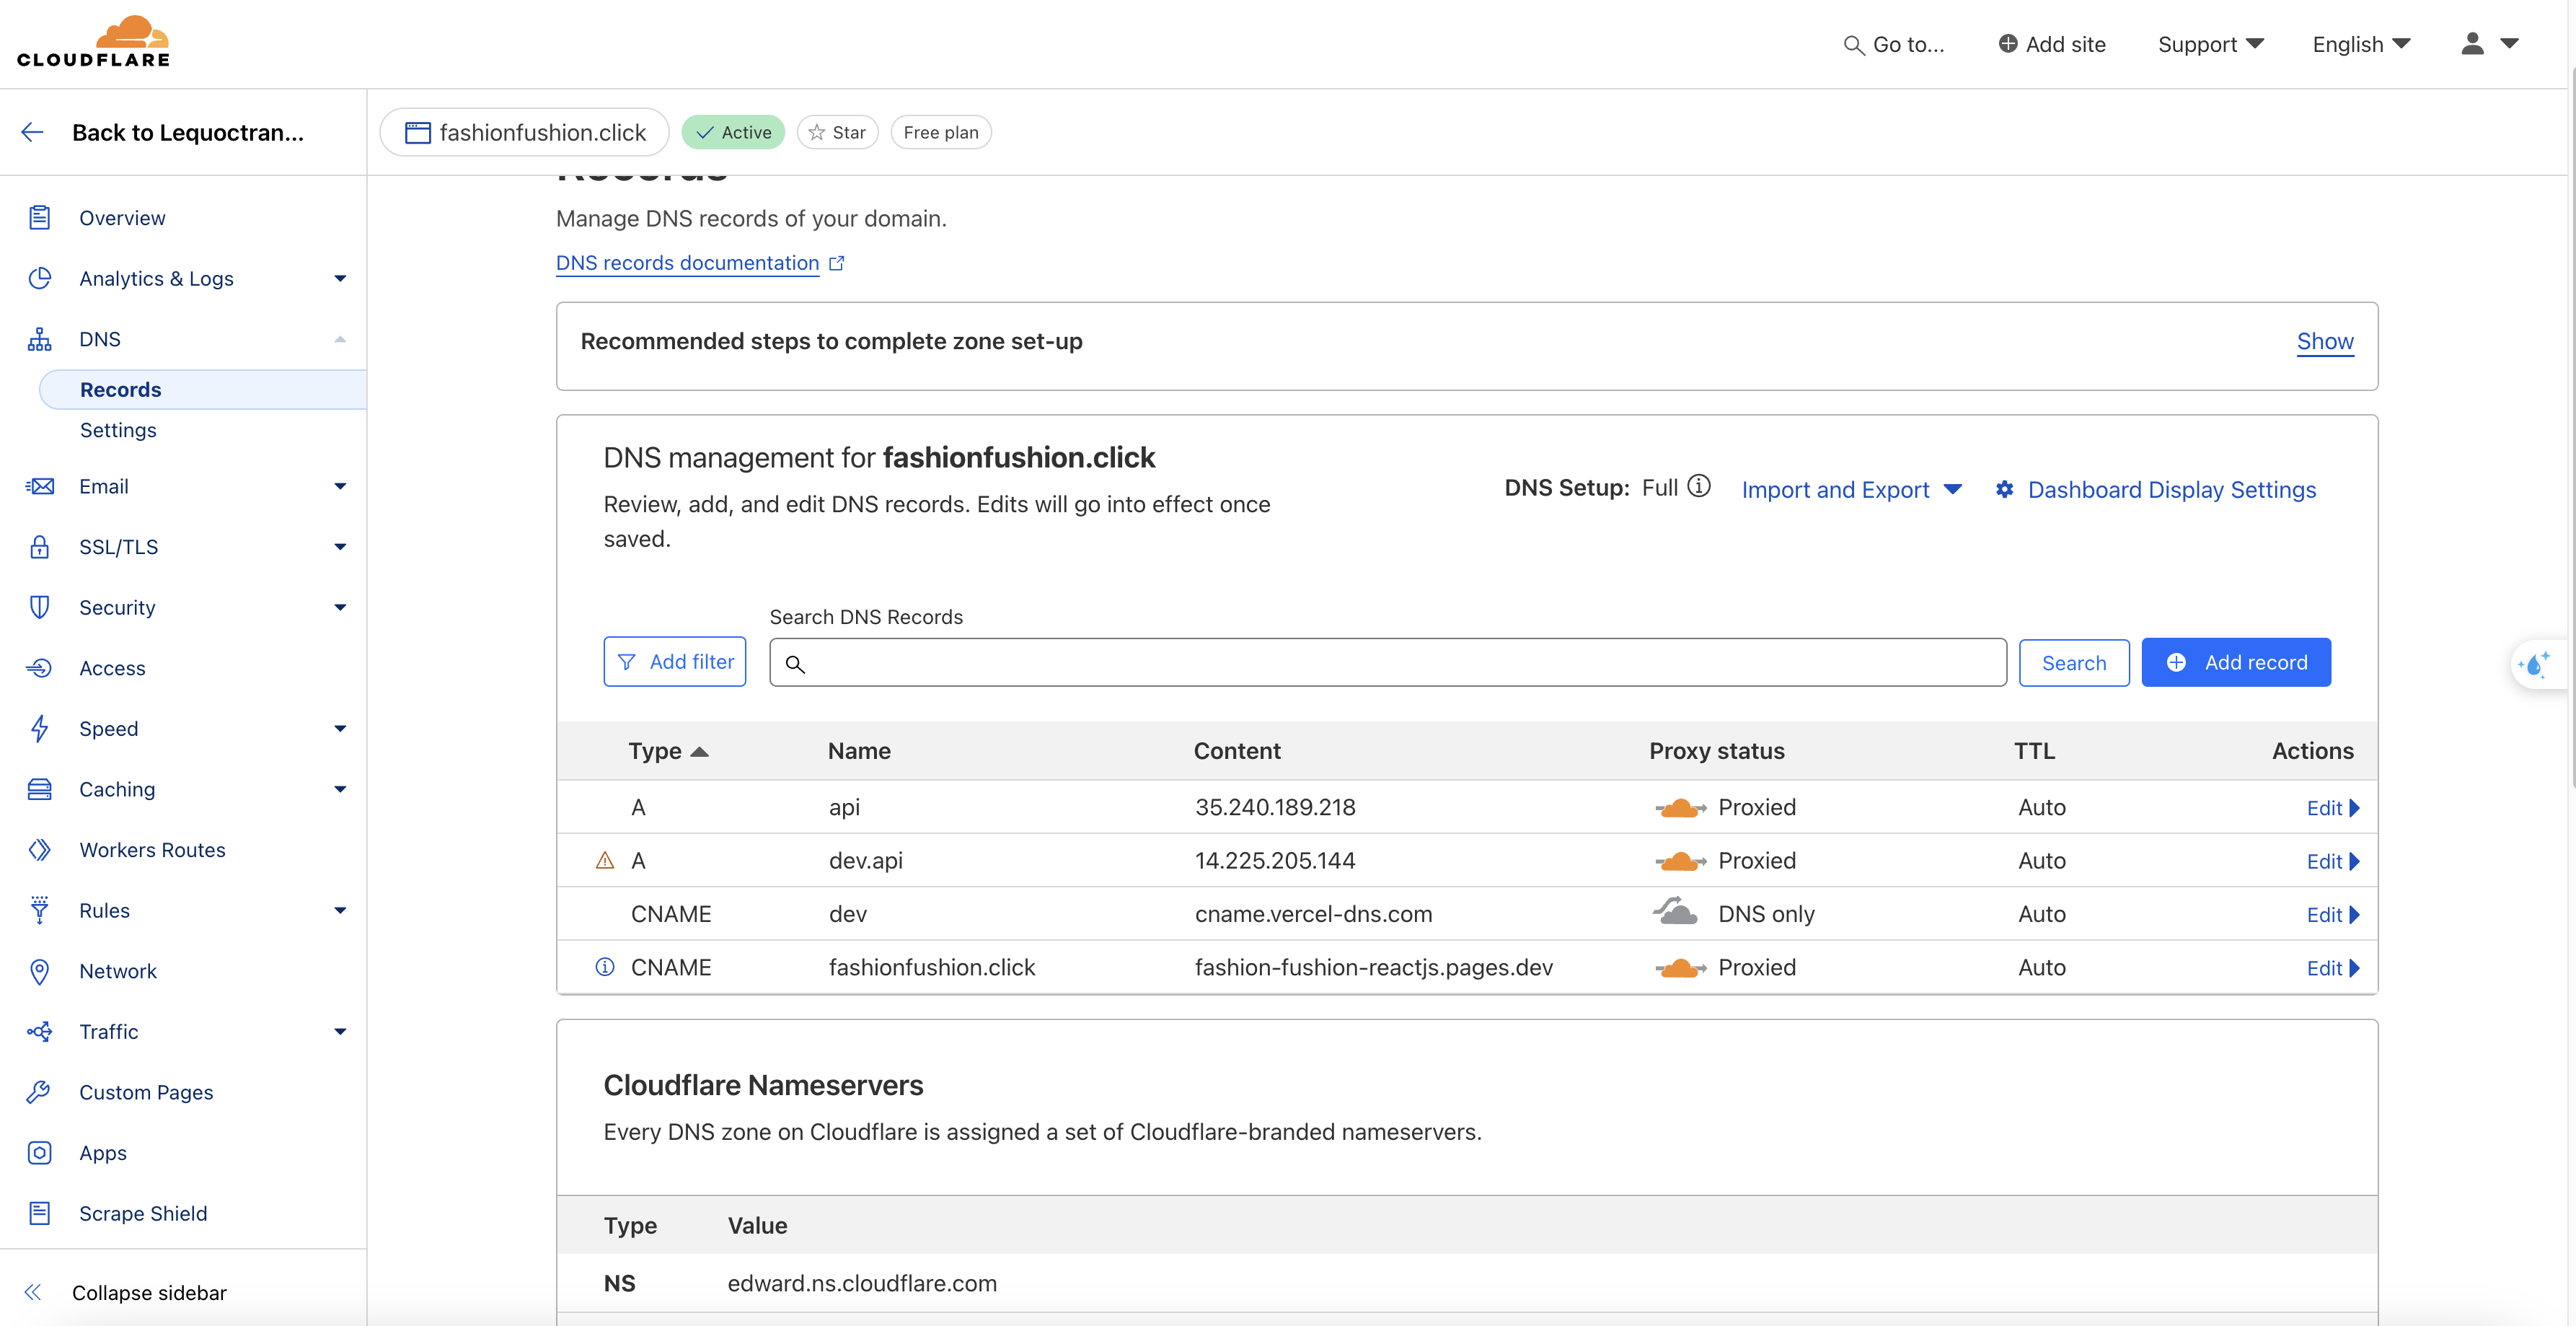
\includegraphics[width=15cm]{Images/Trienkhai/dns.png}
    \newline
    \caption{Thiết lập DNS cho tên miền}
\end{figure}
Sau khi thực hiện thiết lập tên miền thì đường dẫn Web service api và trang web như sau:
\begin{itemize}
    \item \textbf{Môi trường develop}: môi trường dành cho nhà phát triển
    \begin{itemize}
        \item Backend Api: https://dev.api.fashionfushion.click
        \item Website Admin: https://dev.fashionfushion.click
    \end{itemize}
    \item \textbf{Môi trường production}: môi trường dành cho thương mại
    \begin{itemize}
        \item Backend Api: https://api.fashionfushion.click
        \item Website Admin: https://fashionfushion.click
    \end{itemize}
\end{itemize}

\subsection{Đánh giá hệ thống}
\subsubsection{Đánh giá hiệu suất hệ thống bằng Google PageSpeed Insights}
Hiệu suất tải trang web là một yếu tố quan trọng đối với trải nghiệm người dùng của các ứng dụng web. Nhận thức được điều này, chúng tôi đã tiến hành đánh giá bằng cách sử dụng công cụ PageSpeed Insights của Google Chrome. PageSpeed Insights không chỉ giúp đánh giá hiệu suất mà còn đưa ra các khuyến nghị để cải thiện tốc độ tải của ứng dụng web. Chúng tôi sử dụng PageSpeed Insights để đánh giá ứng dụng web đã được triển khai trên Cloudflare.\\
 \begin{figure}[H]
        \centering
        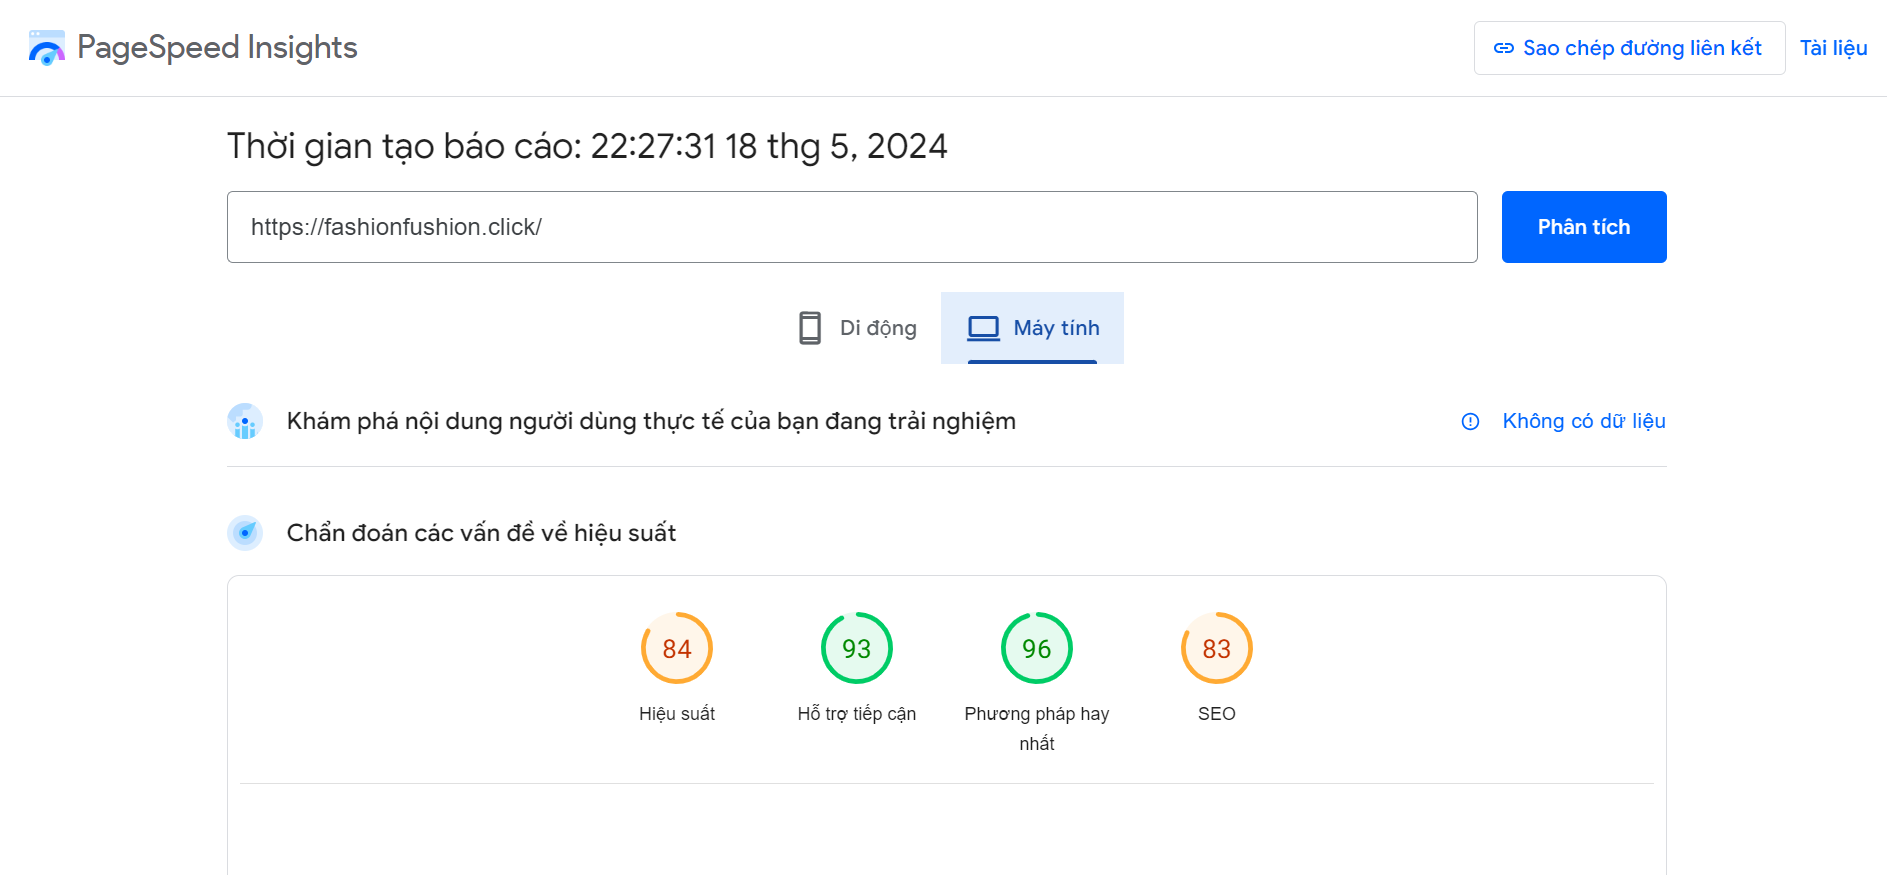
\includegraphics[width=16cm]{Images/hieusuat.png}
        \newline
        \caption{Điểm đánh giá PageSpeed Insights lần đầu tiên}
    \end{figure}
\newpage


\section{Tổng kết, đánh giá và hướng phát triển đề tài}
\subsection{Đánh giá kết quả đạt được}
\subsubsection{Đối với nhiệm vụ của đề tài}
\begin{enumerate}[-]
    \item Tìm hiểu các nghiệp vụ và tìm kiếm các tính năng hữu ích để xây dựng ứng dụng bán hàng thời trang và trang quản lý bán hàng.
    \item Tìm hiểu và vận dụng các kỹ năng lập trình front-end website để tạo ra những giao diện hiện đại, dễ dàng sử dụng, đẹp mắt.
    \item Tìm hiểu, học hỏi và vận dụng kĩ năng lập trình mobile app để xây dựng ứng dụng cho người dùng có thể mua hàng, nhận thông báo mua hàng.
    \item Tìm hiểu, học hỏi và vận dụng kĩ năng lập trình back-end để xây dựng server bán hàng thời trang
    \item Tích hợp API với các bên thứ ba để xây dựng tiện ích gửi mail thông báo cho người dùng và áp dụng thanh toán trực tuyến.
    \item Triển khai server ở Google Cloud, và trang web quản lý ở CloudFare. Bên cạnh đó còn cấu hình tên miền cho server và trang web
    \item Triển khai thành công ứng dụng mobile mua hàng dưới dạng file APK và IOS.
\end{enumerate}
\subsubsection{Đối với cơ sở lý thuyết và công nghệ}
Để hiện thực hệ thống, chúng tôi tìm hiểu các công nghệ phù hợp với những yêu cầu nghiệp vụ. Qua quá trình đó, chúng tôi có cơ hội tìm tòi, học hỏi những công nghệ phát triển web, ứng dụng di động và công nghệ hiện thực cho máy chủ, cụ thể như sau:
\begin{enumerate}[-]
    \item Đối với web, chúng tôi đã sử dụng ReactJS kèm theo Redux cho việc quản lý state, cách triển khai ứng dụng React 
    \item Đối với ứng dụng di động, chúng tôi đã sử dụng React Native kèm theo Redux cho việc quản lý state, React Query cho việc lưu trữ dữ liệu tạm thời API
    \item  Đối với server back-end, chúng tôi hiện thực bằng ExpressJS, sử dụng Postgres lưu trữ cơ sở dữ liệu và Neo4j để lưu trữ dữ liệu dưới dạng quan hệ. Ngoài ra còn 1 server để được hiện thực bằng Fast API (Python) dùng cho việc phân tích hình ảnh, kèm theo đó là tích hợp các dịch vụ hỗ trợ việc triển khai hệ thống:
    \begin{enumerate}[+]
        \item Dịch vụ cung cấp tên miền: TenTen
        \item Dịch vụ Email: Google
        \item Dịch vụ lưu trữ: AWS S3
        \item Dịch vụ thanh toán đa năng: PayOS
    \end{enumerate}
\end{enumerate}
\subsubsection{Đối với quy trình phát triển phần mềm}
Từ những nền tảng công nghệ, chúng tôi tiến hành thực hiện những bước để phát triển hệ thống:
\begin{enumerate}[-]
    \item Tìm hiểu nghiệp vụ và phân tích các chức năng có trong hệ thống.
    \item Thiết kế cơ sở dữ liệu, và kiến trúc hệ thống
    \item Thiết kế giao diện người dùng Figma
    \item Hiện thực hệ thống bao gồm server, web và ứng dụng di động
    \item Kiểm thử hệ thống
    \item Triển khai hệ thống
\end{enumerate}
\subsubsection{Đối với lợi ích thực tế}
\begin{enumerate}[-]
    \item Trải nghiệm mua sắm tốt hơn cho người dùng: Các tính năng gợi ý sản phẩm và tìm kiếm bằng hình ảnh giúp cải thiện trải nghiệm mua sắm của người dùng. Thay vì phải tìm kiếm sản phẩm thủ công, người dùng có thể nhận được gợi ý sản phẩm phù hợp dựa trên sở thích và lựa chọn của họ.
\end{enumerate}
\subsection{Những thuận lợi và khó khăn trong việc thực hiện đề tài}
\subsubsection{Thuận lợi}
\begin{itemize}
    \item \textbf{Sự hỗ trợ từ giảng viên hướng dẫn}
\end{itemize}
  Với sự tận tâm và kiến thức chuyên môn của thầy Phan Trọng Nhân, thầy đã hỗ trợ, hướng dẫn và giúp nhóm định hướng trong quá trình thực hiện đề tài. Đây là nguồn động lực rất lớn giúp nhóm vượt qua những khó khăn để hoàn thành tốt đề tài.
 
\begin{itemize}
    \item \textbf{Tinh thần đồng đội và khả năng làm việc nhóm}
\end{itemize}
Trong quá trình thực hiện đề tài, tinh thần đồng đội mạnh mẽ đã giúp chúng tôi làm việc một cách hiệu quả hơn bằng cách chia sẻ kiến thức và kinh nghiệm. Mỗi thành viên trong nhóm không ngừng hỗ trợ lẫn nhau, đồng thời tôn trọng và đánh giá cao những đóng góp của từng thành viên. Điều này giúp chúng tôi vượt qua những thách thức và khó khăn trong quá trình thực hiện, tạo điều kiện cho sự thành công của đề tài.
\subsubsection{Khó khăn}
\begin{itemize}
    \item \textbf{Tính phức tạp của hệ thống thời trang}
\end{itemize}
Việc tìm hiểu và áp dụng các phương pháp quản lý hiệu quả trong ngành công nghiệp thời trang đòi hỏi đòi hỏi sự kết hợp giữa kiến thức về quản lý kinh doanh và sự hiểu biết sâu sắc về ngành công nghiệp thời trang. Ngoài ra, việc tích hợp công nghệ vào quá trình quản lý và hỗ trợ bán hàng cũng đòi hỏi sự đầu tư, tinh chỉnh liên tục để đảm bảo tính hiệu quả trong hoạt động kinh doanh thời trang.
\begin{itemize}
    \item \textbf{Thiếu nguồn lực và thiếu kinh nghiệm}
\end{itemize}
Việc phát triển hệ thống đã gặp một số khó
khăn về nguồn lực, điều này đã hạn chế khả năng phát triển hệ thống. Bên cạnh đó, sự thiếu kinh nghiệm trong lĩnh vực quản lý và bán hàng thời trang đã làm chậm quá trình tiến hành và yêu cầu chúng tôi phải tìm hiểu và học hỏi nhanh chóng từ các nguồn tài liệu và thực tiễn.
\subsection{Hướng phát triển đề tài}
Với phiên bản hiện tại, nhóm chúng tôi xin đề xuất một số hướng phát triển và mở rộng cho hệ thống nếu sau này:
\begin{enumerate}[-]
\item Ứng dụng công nghệ thực tế ảo (VR) và thực tế tăng cường (AR): Tạo ra các phòng thử đồ ảo, giúp khách hàng có thể thử trang phục mà không cần đến trực tiếp cửa hàng.
\item Chatbot và dịch vụ khách hàng tự động: Phát triển các chatbot thông minh có khả năng trả lời các câu hỏi thường gặp của khách hàng, hỗ trợ trong quá trình mua sắm và xử lý các vấn đề phát sinh một cách nhanh chóng.
\item Tích hợp trí tuệ nhân tạo (AI): Sử dụng AI để phân tích dữ liệu khách hàng, dự đoán xu hướng thời trang và cá nhân hóa trải nghiệm mua sắm của từng khách hàng. AI có thể giúp đề xuất sản phẩm phù hợp với sở thích và lịch sử mua sắm của khách hàng.
\item Tính năng tư vấn thời trang: Cung cấp dịch vụ tư vấn thời trang trực tuyến thông qua các chuyên gia hoặc AI, giúp khách hàng lựa chọn trang phục phù hợp với phong cách và nhu cầu cá nhân.
\item Tích hợp các hình thức thanh toán liên kết thẻ ngân hàng, thẻ tín dụng, Visa để người dùng có thể thanh toán chỉ bằng 1 chạm.

\end{enumerate}
\newpage


\bibliographystyle{plain}
\bibliography{references}
\end{document}